\documentclass[11pt,letterpaper]{article}
\usepackage{graphicx, geometry, amsmath, amssymb, url, booktabs, xcolor, array, longtable, float, caption}
\usepackage[hidelinks]{hyperref}
\usepackage{xurl}
\usepackage{pdflscape}
\geometry{margin=1in}
\captionsetup{font=small,labelfont=bf}
\captionsetup[table]{justification=raggedright,singlelinecheck=false}
\setlength{\LTcapwidth}{\linewidth}
\newenvironment{correction}{\par\medskip\noindent\begin{minipage}{\linewidth}\setlength{\fboxsep}{6pt}\begin{lrbox}{0}\begin{minipage}{0.96\linewidth}\small}{\end{minipage}\end{lrbox}\colorbox{black!6}{\usebox{0}}\end{minipage}\par\medskip}
\emergencystretch=3em
\sloppy
\title{Gold-free checks of whether a logic formula matches its sentence\\[4pt]\large Internal research report: the run's chronological record}
\author{Research log of the NL$\rightarrow$FOL faithfulness-metric run}
\date{24 September 2026}
\begin{document}
\maketitle
\tableofcontents
\clearpage
\section{How this record is organised}

This document is the run's internal research report, typeset from the run's own report text and checked against the artifacts' output files. It is chronological. Section 2 sets out the problem as the run framed it. Section 3 is iteration 1: the hypothesis review, the pre-registered screen, its two screen arms and the held-out dataset. Section 4 is the second iteration of an earlier run of the same project, which tested the iteration-1 candidates on held-out data; it is carried in verbatim because the conclusions after iteration 1 were drawn from it. Section 5 is the closing record written at the end of iteration 1, kept as written with corrections marked in place. Section 6 is iteration 2 of this run, ending with the reviewer's verdict on it and the hypothesis update it produced. Section 7 states what the run learned overall and what is still open.

Tables keep the numbering of the run's own report (Tables 1 to 62 for this run, Tables 126 to 151 for the carried-in round 2), because the prose cites them by those numbers. Tables that the run's report printed without a number, and tables added for this typeset record from the artifacts' output files, carry a letter suffix (for example Table 2a). Every table caption ends with the artifact and iteration it came from. Corrections made in iteration 2 to earlier text appear in shaded boxes.

\begin{table}[H]
\centering
\scriptsize
\setlength{\tabcolsep}{3pt}
\caption*{\textbf{Table 0a.} Run bookkeeping, one row per iteration, from the run's trajectory log. ``Ledger spend'' is the LLM, tool and container spend billed to this run's ledger, cumulative through that iteration; it excludes compute-rental time and is not the run's total cost. The iteration-1 figure is far below the \$16.44 of API spend that the iteration-1 artifacts record (Section 3.7); those artifacts ran in the earlier run's workspace. \textit{[Source: this run's trajectory log (both iterations)]}}
\begin{tabular}{>{\raggedright\arraybackslash}p{0.096\linewidth}>{\raggedright\arraybackslash}p{0.106\linewidth}>{\raggedright\arraybackslash}p{0.051\linewidth}>{\raggedright\arraybackslash}p{0.065\linewidth}>{\raggedright\arraybackslash}p{0.086\linewidth}>{\raggedright\arraybackslash}p{0.170\linewidth}>{\raggedright\arraybackslash}p{0.086\linewidth}>{\raggedright\arraybackslash}p{0.086\linewidth}>{\raggedright\arraybackslash}p{0.130\linewidth}}
\toprule
\textbf{Iteration} & \textbf{Hypothesis state after the iteration} & \textbf{Move} & \textbf{Review score} & \textbf{Executed} & \textbf{Artifacts executed} & \textbf{Evidence state} & \textbf{Coverage} & \textbf{Ledger spend (USD, cumulative)} \\
\midrule
{}1 & Where a formula sits among its peers & deepen & 4 & yes & \texorpdfstring{\textup{\nolinkurl{gen_art_experiment_1}}}{gen art experiment 1}, \texorpdfstring{\textup{\nolinkurl{gen_art_experiment_2}}}{gen art experiment 2} & lead & full & 0.3405895 \\
{}2 & Peer agreement, checked by a cheap judge & deepen & 5 & yes & \texorpdfstring{\textup{\nolinkurl{gen_art_experiment_3}}}{gen art experiment 3}, \texorpdfstring{\textup{\nolinkurl{gen_art_experiment_4}}}{gen art experiment 4}, \texorpdfstring{\textup{\nolinkurl{gen_art_experiment_5}}}{gen art experiment 5} & lead & partial & 36.4956844724489 \\
\bottomrule
\end{tabular}
\end{table}

The trajectory log also records, per iteration, the state of each strand. After iteration 1 it marked the monotonicity signature (the Arm A artifact) as null, cross-system latent class (the Arm B artifact) as a lead, and the dataset's label findings as a lead. After iteration 2 it marked the fresh confirmation and the development stress test as leads and the legal-text test as null.

\begin{table}[H]
\centering
\footnotesize
\setlength{\tabcolsep}{3pt}
\caption*{\textbf{Table 0b.} Every artifact of the run, the iteration that produced it, where in this document it is reported, and the files its numbers were read from. The iteration-1 artifacts ran in the earlier run's workspace; the round-2 artifacts of Section 4 belong to the earlier run and are listed separately in Section 4. \textit{[Source: artifact workspaces listed for this run (iterations 1 and 2)]}}
\begin{tabular}{>{\raggedright\arraybackslash}p{0.193\linewidth}>{\raggedright\arraybackslash}p{0.114\linewidth}>{\raggedright\arraybackslash}p{0.098\linewidth}>{\raggedright\arraybackslash}p{0.193\linewidth}>{\raggedright\arraybackslash}p{0.102\linewidth}>{\raggedright\arraybackslash}p{0.212\linewidth}}
\toprule
\textbf{Artifact} & \textbf{Iteration} & \textbf{Type} & \textbf{What it did} & \textbf{Reported in} & \textbf{Main output files} \\
\midrule
{}\texorpdfstring{\textup{\nolinkurl{gen_art_experiment_1}}}{gen art experiment 1} & 1 & experiment & Screen Arm A: the monotonicity signature and its controls on 835 Logic-LM candidates & Section 3.3 & \texttt{method.py}, \texttt{full\_\allowbreak{}\allowbreak{}method\_\allowbreak{}\allowbreak{}out.json}, \texttt{results/\allowbreak{}summary.json}, \texttt{results/\allowbreak{}screen\_\allowbreak{}\allowbreak{}scores.jsonl} \\
{}\texorpdfstring{\textup{\nolinkurl{gen_art_experiment_2}}}{gen art experiment 2} & 1 & experiment & Screen Arm B: truth-value-judgment worlds, instance-consequence NLI, latent-class agreement & Section 3.4 & \texttt{full\_\allowbreak{}\allowbreak{}method\_\allowbreak{}\allowbreak{}out.json}, \texttt{results/\allowbreak{}screen\_\allowbreak{}\allowbreak{}scores.jsonl}, \texttt{analysis.json}, \texttt{verdict.json} \\
{}\texorpdfstring{\textup{\nolinkurl{gen_art_dataset_1}}}{gen art dataset 1} & 1 & dataset & Held-out meta-evaluation set, 15,606 rows, with panel and solver labels & Section 3.6 & \texttt{full\_\allowbreak{}\allowbreak{}data\_\allowbreak{}\allowbreak{}out/\allowbreak{}}, \texttt{label\_\allowbreak{}\allowbreak{}report.json}, \texttt{README.md} \\
{}\texorpdfstring{\textup{\nolinkurl{gen_art_experiment_3}}}{gen art experiment 3} & 2 & experiment & Freeze-then-confirm test of directional consensus on 450 fresh sentences & Section 6.3 & \texttt{results/\allowbreak{}tests.json}, \texttt{results/\allowbreak{}analysis.json}, \texttt{results/\allowbreak{}report\_\allowbreak{}\allowbreak{}tables.md}, \texttt{results/\allowbreak{}fresh\_\allowbreak{}\allowbreak{}set.jsonl} \\
{}\texorpdfstring{\textup{\nolinkurl{gen_art_experiment_4}}}{gen art experiment 4} & 2 & experiment & Directional consensus under constructed truth on the development set & Section 6.2 & \texttt{results/\allowbreak{}m0\_\allowbreak{}\allowbreak{}anchor.json} to \texttt{results/\allowbreak{}m7\_\allowbreak{}\allowbreak{}goldflag.json}, \texttt{results/\allowbreak{}verdicts.json} \\
{}\texorpdfstring{\textup{\nolinkurl{gen_art_experiment_5}}}{gen art experiment 5} & 2 & experiment & Directional consensus on 158 long legal definitions & Section 6.4 & \texttt{results/\allowbreak{}tests.json}, \texttt{results/\allowbreak{}analysis.json}, \texttt{results/\allowbreak{}exception\_\allowbreak{}\allowbreak{}set.jsonl} \\
\bottomrule
\end{tabular}
\end{table}

\section{Framing}

This run looks for metrics that say whether a first-order logic (FOL) formula is a faithful translation of a natural-language sentence, when no gold formula is available. The setting comes from the user. They build NL-to-FOL pipelines with large language models (LLMs), and their evaluation stalls on two points. First, gold FOL is scarce and not unique: different predicate names, different decompositions of one concept, and logically equivalent rewrites can all be correct. Second, their own pilot metrics measure only stability and composability, not meaning. Those metrics were joint loadability, arity consistency, undefined predicates, and predicate-set overlap across reruns. The target is fixed in advance. A metric has to predict faithfulness to the text on real system outputs, and ideally name the error type. Detecting synthetic perturbations, parse validity and run-to-run stability do not count as substitutes. Every metric is compared with parse rate, round-trip similarity, LLM-as-a-judge, sampling self-consistency and the user's structural metrics. Results are reported by sentence complexity, because long, heavily conditioned sentences matter most to the user.

The public benchmarks that supply gold are themselves unreliable. FOLIO [1], MALLS [2] and ProverQA [3] carry sentence-level FOL annotations. A 2026 relabelling study reports that about 42.5\% of FOLIO-validation and 42\% of MALLS-test entries contain incorrect formalizations, and that 17.8\% and 51\% of their sentences are ambiguous [4]. The gold-free methods already in use compare a whole formula, or its back-translation, with the text through an LLM. Examples are round-trip verification [5], clause-conformance scoring [6] and LLM-as-a-judge [7]. A trained reference-free verifier, GenV, reaches 0.961 AUROC on reference-equivalence verification [8]; its task is to predict equivalence to a designated reference, not faithfulness to the text. The closest gold-based ancestor of the run's main idea is the polarity evaluation of SyGNS [9], which compares per-word monotonicity marks of a predicted formula with those of the gold. A second relative matches NL-derived probes against the formal consequences of a statement [10]. The systems whose outputs are scored here are the Logic-LM [11] and LINC-style [12] pipelines: an LLM translates, and a prover or solver such as Z3 [13] reasons.

\begin{correction}\textbf{Correction (iteration 2).} The 42.5\% / 42\% and 17.8\% / 51\% figures are those of version 2 of arXiv:2606.02837. Version 1, whose abstract the hypothesis quotes, reports 39\% / 36\% incorrect formalizations and 16.4\% / 48\% ambiguous sentences. Both versions are tabulated in Table 38 \footnote{Code: \url{https://github.com/ai-inventor-papers/ai-invention-abf543-do-sentence-and-formula-generalize-the/tree/main/round-2/experiment-4}}.\end{correction}

The run also leans on four other lines of work. First, semantic evaluation of logical forms. Test-suite accuracy for text-to-SQL [21] and its formal-verification critique [35] compare denotations with a gold query, and a perturbation study of FOL closeness metrics [20] measures how gold-based scores react to typed edits. The run reuses typed perturbations only as a diagnostic instrument. Second, distinguishing inputs judged by an LLM: this idea is established for code and SQL [24, 25] and for formal specifications [26], and it is the mechanism behind the truth-value-judgment alternate. Third, agreement among samples. Self-consistency [30], symbolic-equivalence consistency in autoformalization [33], SAT-based selection among compositional translations [31] and grammar-based uncertainty measures [32] all score agreement within a generator's own distribution rather than agreement with the text. Entailment-preserving FOL metrics [34] are reference-free but need multi-premise NLI labels. Fourth, estimation without a gold standard. Latent-class models of rater error [22, 23] come from epidemiology, where they are known to be biased when the tests' errors are conditionally dependent [36]; gold-free benchmarking of LLM judgments has also been proposed [37]. Sentence embeddings for round-trip similarity use Sentence-BERT-style encoders [28] with MiniLM [29].

The hypothesis the run started from is that a formula is faithful only if it shares the sentence's \emph{monotonicity signature}. We use the hypothesis's own definition throughout. For every concept the sentence mentions, the signature records whether the sentence stays true when the concept is generalized (upward), specialized (downward), both (vacuous) or neither. It also records which concept fills each argument slot of each relation (\emph{role anchoring}). On the formula side a solver decides these labels exactly over small finite domains. On the sentence side a formula-blind \emph{substitution probe} asks an LLM whether the sentence entails copies of itself with one concept specialized. The probe was validated independently on the monotonicity NLI sets MED [14] and HELP [15], and the zero-LLM variant uses rule-based polarity marking [16, 17]. The idea borrows from generalized-quantifier theory [18] and from vacuity detection in model checking [19]. Three alternates were carried from the start:

\begin{itemize}
\item {}\emph{truth-value-judgment worlds}: a solver builds small worlds that separate a candidate from its mutants, and an LLM judges only whether the sentence is true in each world;
\item {}\emph{instance-consequence NLI}: a small NLI model checks prover-derived ground consequences against the sentence;
\item {}\emph{latent-class estimation}: the outputs of several systems are treated as imperfect diagnostic tests.
\end{itemize}
The run allows two iterations. This document records them in order.

\section{Iteration 1}

\subsection{Where the iteration started: the hypothesis review}

Before the invention loop began, a reviewer scored the hypothesis 5/10 (soundness 2, presentation 3, contribution 3, fidelity 4). The blocking flag was set only because no experiment had run yet. The reviewer ran the hypothesis's own Z3 prototype and found four common error classes to which the plain signature is blind:

\begin{itemize}
\item {}conjunction/disjunction confusion in the restrictor;
\item {}conjunction/disjunction confusion in the scope;
\item {}consequents swapped under an exception;
\item {}swapped constants.
\end{itemize}
Exception concepts also collapsed to the non-monotone label. Since these errors sit in exactly the long, exception-laden sentences the complexity prediction is about, the reviewer argued that per-concept coordinates lose information where the run hoped they would gain it.

The reviewer made four further objections:

\begin{enumerate}
\item {}Invariance ``by construction'' holds for the solver core only. A lexical aligner reintroduces vocabulary sensitivity: a compound predicate such as \texttt{UntrainedDog} aligned to ``trained'' raises a false polarity alarm.
\item {}The planned granularity-aware label reused name alignment, which couples the labels to the metric.
\item {}SyGNS [9], GenV [8] and the probe-matching work [10] were uncited.
\item {}Nothing in the plan measured what fraction of real errors change the signature at all.
\end{enumerate}
The reviewer asked for three additions: an oracle-ceiling condition that uses the gold formula's signature in place of the text probe; a decomposed-judge ablation, which asks an LLM the same per-concept questions about the formula; and label construction independent of the metric's aligner. The reviewer also verified a repair, the \emph{relativized signature}: the monotonicity of predicate P when P may change only inside, or only outside, another predicate Q. The relativized signature separated all three failing pairs with 6 to 8 differing coordinates, and it gave 0 differences on a contrapositive rewrite.

\subsection{Strategy: a pre-registered wide screen plus a held-out dataset}

With four live candidate metrics and two iterations, the strategy step chose a wide screen over depth. It had two reasons. The candidates see different errors, so real outputs had to decide between them. The signature is local and depends on alignment. The world-based checks are global and alignment-free but depend on verbalizing predicate names. The latent-class model ignores the text entirely. If real errors were mostly scope errors, the world-based checks should win; if they were mostly polarity or condition errors on long sentences, the signature should win. Second, a held-out labelled set that was not built in iteration 1 could not be built later, so one of the three artifact slots went to a dataset.

Iteration 1 therefore ran three artifacts in parallel. Screen Arm A (artifact \texorpdfstring{\textup{\nolinkurl{gen_art_experiment_1}}}{gen art experiment 1}) tested the signature variants. Screen Arm B (artifact \texorpdfstring{\textup{\nolinkurl{gen_art_experiment_2}}}{gen art experiment 2}) tested the three alternates. A dataset artifact (\texorpdfstring{\textup{\nolinkurl{gen_art_dataset_1}}}{gen art dataset 1}) built a held-out confirmation set for iteration 2. Both screen arms rebuilt one frozen screen set from public sources with an identical deterministic recipe:

\begin{itemize}
\item {}the Logic-LM released translations of FOLIO-dev by gpt-3.5-turbo, gpt-4 and text-davinci-003 [11];
\item {}gold from FOLIO validation [1], with the 2606.02837 corrections [4] where retrievable;
\item {}the first 300 matched sentences in sha1 order;
\item {}labels from blind Z3 equivalence up to an arity-preserving bijection of predicates and constants, searched without lexical information.
\end{itemize}
Typed mutants and solver-verified meaning-preserving rewrites of each gold served as gates and mechanism diagnostics, never as the headline.

The selection rule was fixed before any score existed and copied verbatim into both arms. The primary measure was the item-level AUROC on the real candidates against the bijection-equivalence labels, with a 1000$\times$ bootstrap clustered by sentence. Table 1 lists the four gates.

\begin{table}[H]
\centering
\small
\setlength{\tabcolsep}{3pt}
\caption*{\textbf{Table 1.} The pre-registered survival gates, fixed before any scores existed. \textit{[Source: iteration-1 strategy, copied into both screen arms (\texorpdfstring{\textup{\nolinkurl{gen_art_experiment_1}}}{gen art experiment 1} and \texorpdfstring{\textup{\nolinkurl{gen_art_experiment_2}}}{gen art experiment 2}), iteration 1]}}
\begin{tabular}{>{\raggedright\arraybackslash}p{0.239\linewidth}>{\raggedright\arraybackslash}p{0.726\linewidth}}
\toprule
\textbf{Gate} & \textbf{Condition} \\
\midrule
{}G1 coverage & at least 70\% of real candidates scored; unscored items get 0.5 and stay in the AUROC \\
{}G2 false alarms & at most 10\% on solver-verified meaning-preserving rewrites \\
{}G3 increment & $\Delta$AUROC of logistic(cheap judge + parse\_\allowbreak{}ok + metric) over logistic(cheap judge + parse\_\allowbreak{}ok), clustered-bootstrap 95\% lower bound $>$ 0 \\
{}G4 AUROC floor & AUROC on real candidates $\geq$ 0.65 \\
\bottomrule
\end{tabular}
\end{table}

Survivors were to be ranked by AUROC on the top complexity tercile, and a winner declared only with a lead of at least 0.03 there. If nothing survived, the candidate with the largest increment point estimate would advance, provided that estimate was at least 0.03. In iteration 2 the rule is to be re-applied with the dataset's audited screen labels, and the audited ranking governs if the two disagree.

The strategy recorded where it broke the field's norms, and why:

\begin{enumerate}
\item {}The screen used unadjudicated equivalence labels on partly uncorrected gold. This is cheap and identical for every candidate. Its known bias, counting correct-but-gold-inequivalent candidates as wrong, works against the granularity-invariant signature.
\item {}The screen's systems date from 2023. The held-out set was meant to shift both the system era and the corpus.
\item {}The screen is powered for $\Delta$AUROC of about 0.06. That is enough to choose a survivor, not to claim a finding.
\item {}Latent-class estimation is thin with three systems.
\end{enumerate}
\subsection{Screen Arm A: the monotonicity signature (\texorpdfstring{\textup{\nolinkurl{gen_art_experiment_1}}}{gen art experiment 1})}

This subsection reports the artifact \texorpdfstring{\textup{\nolinkurl{gen_art_experiment_1}}}{gen art experiment 1}.\footnote{Code: \url{https://github.com/ai-inventor-papers/ai-invention-abf543-do-sentence-and-formula-generalize-the/tree/main/round-1/experiment-1}}

\subsubsection{What was built}

The formula side parses FOLIO syntax and grounds each formula propositionally. A single SAT query covers every domain size from 1 to N at once, using an active-element encoding. With N = 3, the run computed 2,645 signatures in 19 s. For each predicate the solver decides upward, downward, vacuous or non-monotone, and it decides slot anchors. The relativized coordinates of the review fix are also computed.

Three candidate metrics share this formula side and differ in the text side:

\begin{itemize}
\item {}\textbf{LLM-probe signature} (row label A1): text labels come from the substitution probe, gemini-2.5-flash with a 1,024-token thinking budget. The probe answers batched upward and downward entailment questions per sentence and never sees a formula.
\item {}\textbf{Relativized signature} (A2): the LLM-probe signature plus relativized coordinates, the review's fix.
\item {}\textbf{Rule-marker signature} (A3): text polarity from a compact rule-based monotonicity marker over a spaCy parse, with zero LLM calls. Udep2Mono [17] could not be installed within the time box.
\end{itemize}
Concepts are aligned to predicates by lemma and camelCase overlap. The aligner has rules for compound heads and lexical negation, with a MiniLM [29] embedding fallback. The score is one minus the weighted fraction of mismatched coordinates. A fixed decision list maps the mismatch pattern to an error type.

Two controls were added that were not in the plan, because a lexical aligner can carry signal of its own. The \emph{alignment-only control} (A0) is the same score with the polarity and anchor coordinates switched off. The \emph{concept-coverage control} (Ccov) is the fraction of sentence concepts that align to any predicate. The baselines were:

\begin{itemize}
\item {}the whole-formula LLM judge (B1): gemini-2.5-flash, thinking off, temperature 0, with a fixed prompt asking for the probability that the FOL is faithful;
\item {}parse rate (B2) and its satisfiable variant;
\item {}round-trip (B3): FOL$\rightarrow$NL by gemini-2.5-flash, scored by MiniLM cosine or by bidirectional DeBERTa-v3-large NLI [27];
\item {}the decomposed judge (B4): the same LLM answers the same per-concept upward/downward questions about the formula;
\item {}the gold-signature oracle (B5): the text signature is replaced by the gold formula's solver signature, giving the ceiling if the text side were perfect;
\item {}probe accuracy on MED and HELP (B6);
\item {}the user's pilot structural metrics (B7);
\item {}self-consistency (B8), added during execution: Logic-LM re-translated each story's premises independently for every example of that story, so the agreement of a candidate with the same system's other translations of the same sentence costs nothing.
\end{itemize}
\subsubsection{Screen set as built by Arm A}

The screen contains 300 sentences and 835 real candidates: gpt-3.5-turbo 265, gpt-4 298, text-davinci-003 272. Of these, 811 parse. Ten gold formulas were excluded as unparseable; all used the character \texttt{'} inside predicate names. The labels are complete: 389 equivalent and 446 non-equivalent, with 0 unlabeled. Bounded (domains 1 to 4) and unbounded Z3 agree on all 389 equivalences.

The corrected gold turned out to be a story-level re-annotation on the Hugging Face Hub (\texttt{DSAVlab-\allowbreak{}UNIUD/\allowbreak{}FOLIO\_\allowbreak{}\allowbreak{}validation-\allowbreak{}curated}). Its sentence text matches FOLIO v0.0 for only 97 of the 300 screen sentences, so the primary label uses the curated gold on those 97 and the original gold elsewhere. The curated release changed 50 of the 97 golds (52\%).

The mutant generator kept 1,375 solver-verified non-equivalent mutants over 9 operators (Table 2a). It also kept 412 solver-verified equivalent rewrites: synonym renaming 142, contrapositive 115, De Morgan 80, reorder 71, prenex 4. The scope-swap operator applied to none of the 300 golds, because FOLIO-dev gold contains no mixed quantifier prefixes.

\begin{table}[H]
\centering
\scriptsize
\setlength{\tabcolsep}{3pt}
\caption*{\textbf{Table 2a.} Solver-verified non-equivalent mutants kept per operator on the 300 screen golds (Arm A). \textit{[Source: Screen Arm A, \texorpdfstring{\textup{\nolinkurl{gen_art_experiment_1}}}{gen art experiment 1}, iteration 1]}}
\begin{tabular}{>{\raggedright\arraybackslash}p{0.112\linewidth}>{\raggedright\arraybackslash}p{0.049\linewidth}>{\raggedright\arraybackslash}p{0.074\linewidth}>{\raggedright\arraybackslash}p{0.112\linewidth}>{\raggedright\arraybackslash}p{0.061\linewidth}>{\raggedright\arraybackslash}p{0.049\linewidth}>{\raggedright\arraybackslash}p{0.112\linewidth}>{\raggedright\arraybackslash}p{0.074\linewidth}>{\raggedright\arraybackslash}p{0.074\linewidth}>{\raggedright\arraybackslash}p{0.061\linewidth}>{\raggedright\arraybackslash}p{0.074\linewidth}}
\toprule
\textbf{Operator} & \textbf{NEG} & \textbf{QUANT} & \textbf{IMPL\_\allowbreak{}REV} & \textbf{DROP} & \textbf{ADD} & \textbf{ARG\_\allowbreak{}SWAP} & \textbf{ANDOR} & \textbf{MERGE} & \textbf{CARD} & \textbf{SCOPE} \\
\midrule
{}kept & 300 & 157 & 124 & 95 & 300 & 102 & 109 & 151 & 37 & 0 \\
\bottomrule
\end{tabular}
\end{table}

Complexity terciles were cut on a composite of token count, quantifier count, nesting depth and condition count. The top tercile holds 286 candidates, of which only 73 are equivalent to gold; the low tercile holds 264, of which 170 are equivalent.

\begin{table}[H]
\centering
\footnotesize
\setlength{\tabcolsep}{3pt}
\caption*{\textbf{Table 2.} Label diagnostics per system (Arm A). The primary labels mix curated and original gold; the second column uses the original gold only. \textit{[Source: Screen Arm A, \texorpdfstring{\textup{\nolinkurl{gen_art_experiment_1}}}{gen art experiment 1}, iteration 1]}}
\begin{tabular}{>{\raggedright\arraybackslash}p{0.225\linewidth}>{\raggedright\arraybackslash}p{0.048\linewidth}>{\raggedright\arraybackslash}p{0.177\linewidth}>{\raggedright\arraybackslash}p{0.184\linewidth}>{\raggedright\arraybackslash}p{0.189\linewidth}>{\raggedright\arraybackslash}p{0.090\linewidth}}
\toprule
\textbf{System} & \textbf{n} & \textbf{equivalent (primary)} & \textbf{equivalent (original gold)} & \textbf{equivalent (lexical bijection)} & \textbf{parse rate} \\
\midrule
{}gpt-3.5-turbo & 265 & 0.453 & 0.523 & 0.434 & 0.966 \\
{}gpt-4 & 298 & 0.550 & 0.623 & 0.527 & 0.980 \\
{}text-davinci-003 & 272 & 0.386 & 0.454 & 0.386 & 0.967 \\
\bottomrule
\end{tabular}
\end{table}

Among the non-equivalent labels, 352 are \emph{vocabulary-shape mismatches}: the candidate's multiset of predicate arities differs from the gold's, so no bijection can exist. That is 79\% of the non-equivalences, and it is where correct-but-gold-inequivalent candidates with a different granularity land. The other non-equivalences are 70 with a bijection but no equivalence, and 24 unparseable. Labels against the original and the curated gold agree on 75\% of the 277 items that have both. Sixty-two items are equivalent to the original gold but not to the curated one, and 4 go the other way. The blind and lexical bijection labels disagree on 12 items. These are reversed implications that a blind predicate swap maps onto the gold.

\subsubsection{Configuration decisions taken during execution}

The probe configuration was chosen on 100 MED items by a pre-registered rule: keep thinking off unless its downward accuracy is below 0.80 and thinking raises it by at least 0.05. Table 3 gives the pilot.

\begin{table}[H]
\centering
\footnotesize
\setlength{\tabcolsep}{3pt}
\caption*{\textbf{Table 3.} Substitution-probe pilot on 100 MED items. Both gemini configurations fell below the 0.70 downward threshold, which pre-registered a switch to gpt-4.1-mini. gpt-4.1-mini was worse, so the switch was not made. \textit{[Source: Screen Arm A, \texorpdfstring{\textup{\nolinkurl{gen_art_experiment_1}}}{gen art experiment 1}, iteration 1]}}
\begin{tabular}{>{\raggedright\arraybackslash}p{0.256\linewidth}>{\raggedright\arraybackslash}p{0.114\linewidth}>{\raggedright\arraybackslash}p{0.099\linewidth}>{\raggedright\arraybackslash}p{0.128\linewidth}>{\raggedright\arraybackslash}p{0.167\linewidth}>{\raggedright\arraybackslash}p{0.149\linewidth}}
\toprule
\textbf{Probe configuration} & \textbf{overall} & \textbf{upward} & \textbf{downward} & \textbf{downward, entailment} & \textbf{downward, neutral} \\
\midrule
{}gemini-2.5-flash, thinking off & 0.68 & 0.88 & 0.48 & 0.36 & 0.60 \\
{}gemini-2.5-flash, thinking 1024 (chosen) & 0.77 & 0.90 & 0.64 & 0.52 & 0.76 \\
{}gpt-4.1-mini, no thinking & 0.59 & 0.86 & 0.32 & 0.24 & 0.40 \\
\bottomrule
\end{tabular}
\end{table}

Before any real-candidate label was used, the text side was tuned on gold, mutant and rewrite behaviour only:

\begin{itemize}
\item {}optional domain nouns and light verbs (person, thing, have, take);
\item {}predicates allowed to align to proper-noun concepts, and constants to noun concepts.
\end{itemize}
The share of golds with a full signature match rose from 0.31 to 0.43; the gold-signature oracle reaches 0.53. The residue is genuine granularity, because FOLIO golds omit content words the sentence contains.

The decomposed judge cost 3.8 times its estimate. Its mutant sample was cut to 20 per operator and its rewrites to 120, and a tuned-judge tier was skipped under the budget rules.

\subsubsection{Main result on real candidates}

Table 4 is the arm's headline table. On the full screen the three signature variants rank above every baseline except the decomposed judge and the oracle. All three have an increment over judge plus parse rate whose confidence interval excludes zero. In the top complexity tercile every metric falls to chance.

{\footnotesize
\setlength{\tabcolsep}{3pt}
\begin{longtable}{>{\raggedright\arraybackslash}p{0.174\linewidth}>{\raggedright\arraybackslash}p{0.078\linewidth}>{\raggedright\arraybackslash}p{0.101\linewidth}>{\raggedright\arraybackslash}p{0.115\linewidth}>{\raggedright\arraybackslash}p{0.087\linewidth}>{\raggedright\arraybackslash}p{0.156\linewidth}>{\raggedright\arraybackslash}p{0.089\linewidth}>{\raggedright\arraybackslash}p{0.087\linewidth}}
\caption*{\textbf{Table 4.} Arm A: all metrics on 835 real candidates (389 equivalent / 446 not), 1000$\times$ sentence-clustered bootstrap. The false-alarm threshold is $\delta$ = 0 for signature-like scores and $\delta$ = 0.10 for continuous scores. ``$\Delta$ best'' is the increment over a logistic stack of judge, parse, round-trip NLI, structural metrics and self-consistency. \textit{[Source: Screen Arm A, \texorpdfstring{\textup{\nolinkurl{gen_art_experiment_1}}}{gen art experiment 1}, iteration 1]}}\\
\toprule
\textbf{Metric} & \textbf{AUROC [95\% CI]} & \textbf{low / mid / top tercile} & \textbf{G1 coverage} & \textbf{G2 false alarms} & \textbf{G3 $\Delta$AUROC over judge+parse [CI]} & \textbf{$\Delta$ best [CI]} & \textbf{\$/item} \\
\midrule
\endfirsthead
\multicolumn{8}{l}{\textit{(continued)}}\\
\toprule
\textbf{Metric} & \textbf{AUROC [95\% CI]} & \textbf{low / mid / top tercile} & \textbf{G1 coverage} & \textbf{G2 false alarms} & \textbf{G3 $\Delta$AUROC over judge+parse [CI]} & \textbf{$\Delta$ best [CI]} & \textbf{\$/item} \\
\midrule
\endhead
\bottomrule
\endlastfoot
{}A1 LLM-probe signature & 0.711 [0.663, 0.756] & 0.726 / 0.739 / 0.507 & 0.86 & 0.131 & +0.084 [0.037, 0.138] & +0.057 [0.022, 0.092] & 0.0009 \\
{}A2 relativized signature & 0.711 [0.662, 0.756] & 0.724 / 0.739 / 0.507 & 0.86 & 0.131 & +0.084 [0.036, 0.138] & +0.056 [0.021, 0.092] & 0.0009 \\
{}A3 rule-marker signature & 0.718 [0.673, 0.763] & 0.757 / 0.737 / 0.508 & 0.88 & 0.143 & +0.093 [0.048, 0.143] & +0.062 [0.029, 0.097] & 0 \\
{}A0 alignment-only control & 0.674 [0.629, 0.715] & 0.694 / 0.665 / 0.519 & 0.86 & 0.133 & +0.067 [0.025, 0.113] & +0.036 [0.008, 0.065] & 0 \\
{}Ccov concept-coverage control & 0.661 [0.616, 0.706] & 0.677 / 0.651 / 0.460 & 0.97 & 0.160 & +0.056 [0.019, 0.099] & +0.024 [0.004, 0.044] & 0 \\
{}B1 whole-formula judge & 0.644 [0.597, 0.693] & 0.680 / 0.623 / 0.533 & 1.00 & 0.308 & n/a & n/a & 0.00002 \\
{}B2 parse rate & 0.527 [0.515, 0.541] & 0.532 / 0.522 / 0.528 & 1.00 & n/a & n/a & n/a & 0 \\
{}B2sat parse + satisfiable & 0.529 [0.517, 0.543] & 0.532 / 0.525 / 0.531 & 1.00 & n/a & +0.000 [$-$0.000, 0.001] & +0.000 [$-$0.001, 0.001] & 0 \\
{}B3cos round-trip MiniLM & 0.614 [0.562, 0.663] & 0.702 / 0.517 / 0.424 & 1.00 & n/a & +0.015 [$-$0.008, 0.038] & +0.000 [$-$0.005, 0.005] & 0.00006 \\
{}B3nli round-trip DeBERTa NLI & 0.660 [0.612, 0.706] & 0.681 / 0.625 / 0.472 & 1.00 & n/a & +0.027 [$-$0.005, 0.060] & +0.031 [0.001, 0.061] & 0.00006 \\
{}B4 decomposed judge & 0.715 [0.665, 0.760] & 0.710 / 0.769 / 0.521 & 0.82 & 0.183 & +0.088 [0.040, 0.142] & +0.064 [0.027, 0.102] & 0.0041 \\
{}B5 gold-signature oracle & 0.741 [0.694, 0.782] & 0.773 / 0.758 / 0.583 & 0.87 & 0.141 & +0.114 [0.065, 0.168] & +0.080 [0.043, 0.117] & n/a \\
{}B7 structural (user pilot) & 0.537 [0.519, 0.557] & 0.561 / 0.533 / 0.545 & 1.00 & n/a & $-$0.002 [$-$0.011, 0.006] & $-$0.002 [$-$0.006, 0.001] & 0 \\
{}B8 self-consistency & 0.608 [0.564, 0.655] & 0.576 / 0.640 / 0.701 & 0.55 & n/a & +0.027 [$-$0.009, 0.066] & +0.028 [0.006, 0.051] & 0 \\
\end{longtable}
}

The result does not hinge on the label choice. Table 5 re-scores the main metrics under the alternative labels. Every metric rises on the 97-sentence subset with curated gold. The ordering, with the signature above the judge, holds under every labelling.

\begin{table}[H]
\centering
\footnotesize
\setlength{\tabcolsep}{3pt}
\caption*{\textbf{Table 5.} AUROC of Arm A metrics under alternative labellings. ``Curated subset'' has 277 candidates on the 97 sentences with curated gold; ``unparseable as 0'' scores unparseable candidates 0 instead of 0.5. \textit{[Source: Screen Arm A, \texorpdfstring{\textup{\nolinkurl{gen_art_experiment_1}}}{gen art experiment 1}, iteration 1]}}
\begin{tabular}{>{\raggedright\arraybackslash}p{0.221\linewidth}>{\raggedright\arraybackslash}p{0.115\linewidth}>{\raggedright\arraybackslash}p{0.131\linewidth}>{\raggedright\arraybackslash}p{0.149\linewidth}>{\raggedright\arraybackslash}p{0.118\linewidth}>{\raggedright\arraybackslash}p{0.179\linewidth}}
\toprule
\textbf{Metric} & \textbf{primary} & \textbf{original gold} & \textbf{lexical bijection} & \textbf{curated subset} & \textbf{unparseable as 0} \\
\midrule
{}A1 LLM-probe signature & 0.711 & 0.712 & 0.717 & 0.760 & 0.716 \\
{}A3 rule-marker signature & 0.718 & 0.714 & 0.725 & 0.782 & 0.723 \\
{}A0 alignment-only & 0.674 & 0.663 & 0.679 & 0.744 & 0.677 \\
{}B1 judge & 0.644 & 0.666 & 0.649 & 0.721 & 0.659 \\
{}B3nli round-trip & 0.660 & 0.654 & 0.656 & 0.755 & 0.675 \\
{}B4 decomposed judge & 0.715 & 0.719 & 0.719 & 0.770 & 0.721 \\
{}B5 oracle & 0.741 & 0.743 & 0.752 & 0.791 & 0.744 \\
{}B8 self-consistency & 0.608 & 0.578 & 0.596 & 0.521 & 0.621 \\
\bottomrule
\end{tabular}
\end{table}

\subsubsection{Invariance: the gate every signature variant failed}

All three variants failed the false-alarm gate, and Table 6 shows where the failures come from. On the 270 purely logical rewrites (reorder, contrapositive, De Morgan, prenex) the signature metrics raised no alarms. Every alarm came from synonym-renamed predicates, where the lexical aligner lost the concept. The whole-formula judge alarmed on 20\% to 40\% of the logical rewrites.

\begin{table}[H]
\centering
\footnotesize
\setlength{\tabcolsep}{3pt}
\caption*{\textbf{Table 6.} False-alarm rate on solver-verified equivalent rewrites, by rewrite kind (Arm A). The decomposed judge was run on a 120-rewrite subsample. \textit{[Source: Screen Arm A, \texorpdfstring{\textup{\nolinkurl{gen_art_experiment_1}}}{gen art experiment 1}, iteration 1]}}
\begin{tabular}{>{\raggedright\arraybackslash}p{0.234\linewidth}>{\raggedright\arraybackslash}p{0.058\linewidth}>{\raggedright\arraybackslash}p{0.086\linewidth}>{\raggedright\arraybackslash}p{0.086\linewidth}>{\raggedright\arraybackslash}p{0.086\linewidth}>{\raggedright\arraybackslash}p{0.118\linewidth}>{\raggedright\arraybackslash}p{0.103\linewidth}>{\raggedright\arraybackslash}p{0.116\linewidth}}
\toprule
\textbf{Rewrite kind} & \textbf{n} & \textbf{A1} & \textbf{A3} & \textbf{A0} & \textbf{B5 oracle} & \textbf{B1 judge} & \textbf{B4 (n)} \\
\midrule
{}synonym rename & 142 & 0.380 & 0.415 & 0.387 & 0.408 & 0.246 & 0.311 (45) \\
{}contrapositive & 115 & 0.000 & 0.000 & 0.000 & 0.000 & 0.400 & 0.065 (31) \\
{}De Morgan & 80 & 0.000 & 0.000 & 0.000 & 0.000 & 0.388 & 0.211 (19) \\
{}reorder & 71 & 0.000 & 0.000 & 0.000 & 0.000 & 0.197 & 0.087 (23) \\
{}prenex & 4 & 0.000 & 0.000 & 0.000 & 0.000 & 0.250 & 0.000 (2) \\
{}all & 412 & 0.131 & 0.143 & 0.133 & 0.141 & 0.308 & 0.183 (120) \\
\bottomrule
\end{tabular}
\end{table}

At $\delta$ = 0 the judge's false-alarm rate is 0.43.

\textbf{Verdict under the pre-registered rule.} No signature variant survives. All pass the coverage gate, the increment gate and the AUROC floor; all fail the false-alarm gate. Under the no-survivor clause the rule-marker signature advances, because its increment point estimate (+0.093) is the largest and exceeds 0.03.

\subsubsection{Diagnosis: which half of the bridge failed}

The design was meant to locate a failure, and it does. The text side is the bottleneck. On MED and HELP (Table 7) the LLM probe's downward accuracy is 0.60. That is well under the 0.80 bar the hypothesis set for itself and under the 0.85 it assumed. Downward entailments are the weak cell: 0.42 correct. The zero-LLM rule marker is scored on 3,401 MED single-span edits. That is a different item set from the LLM's 400, so the comparison is not exact, but the marker reaches 0.87 overall and 0.86 downward.

\begin{table}[H]
\centering
\footnotesize
\setlength{\tabcolsep}{3pt}
\caption*{\textbf{Table 7.} Text-side accuracy on the monotonicity NLI sets (B6). \textit{[Source: Screen Arm A, \texorpdfstring{\textup{\nolinkurl{gen_art_experiment_1}}}{gen art experiment 1}, iteration 1]}}
\begin{tabular}{>{\raggedright\arraybackslash}p{0.166\linewidth}>{\raggedright\arraybackslash}p{0.066\linewidth}>{\raggedright\arraybackslash}p{0.113\linewidth}>{\raggedright\arraybackslash}p{0.123\linewidth}>{\raggedright\arraybackslash}p{0.139\linewidth}>{\raggedright\arraybackslash}p{0.162\linewidth}>{\raggedright\arraybackslash}p{0.131\linewidth}}
\toprule
\textbf{Set} & \textbf{n} & \textbf{overall} & \textbf{upward} & \textbf{downward} & \textbf{downward entailment} & \textbf{downward neutral} \\
\midrule
{}MED + HELP, LLM probe & 400 & 0.738 & 0.875 & 0.600 & 0.420 & 0.780 \\
{}MED, LLM probe & 300 & 0.763 & 0.900 & 0.627 & 0.467 & 0.787 \\
{}HELP, LLM probe & 100 & 0.660 & 0.800 & 0.520 & 0.280 & 0.760 \\
{}MED single-span edits, rule marker & 3,401 & 0.870 & 0.890 (n=1,346) & 0.856 (n=2,055) & n/a & n/a \\
\bottomrule
\end{tabular}
\end{table}

The same ordering shows up on the screen's own gold formulas. The text-side labels were compared with the gold formula's solver labels on the aligned concepts. The rule marker agreed on 87.2\% of 499 concepts and the LLM probe on 78.3\% of 442. Both do well on upward and downward concepts. On concepts the gold marks non-monotone, the LLM probe agreed on only 17.5\% (n = 40) and the marker on 69.6\% (n = 46).

The contrasts in Table 8 carry the rest of the diagnosis.

{\small
\setlength{\tabcolsep}{3pt}
\begin{longtable}{>{\raggedright\arraybackslash}p{0.655\linewidth}>{\raggedright\arraybackslash}p{0.310\linewidth}}
\caption*{\textbf{Table 8.} Paired AUROC contrasts on real candidates (Arm A), sentence-clustered 95\% CIs. The last four rows are increments over a logistic stack of [judge, parse\_\allowbreak{}ok, alignment-only control]. \textit{[Source: Screen Arm A, \texorpdfstring{\textup{\nolinkurl{gen_art_experiment_1}}}{gen art experiment 1}, iteration 1]}}\\
\toprule
\textbf{Contrast} & \textbf{$\Delta$AUROC [95\% CI]} \\
\midrule
\endfirsthead
\multicolumn{2}{l}{\textit{(continued)}}\\
\toprule
\textbf{Contrast} & \textbf{$\Delta$AUROC [95\% CI]} \\
\midrule
\endhead
\bottomrule
\endlastfoot
{}B5 oracle $-$ A1 (text-side gap) & +0.030 [0.005, 0.058] \\
{}A1 $-$ B4 (exact semantics vs decomposition, n = 810) & $-$0.005 [$-$0.024, 0.014] \\
{}A3 $-$ A1 & +0.007 [$-$0.024, 0.039] \\
{}A1 $-$ A0 (polarity over alignment) & +0.037 [0.006, 0.069] \\
{}A2 $-$ A0 & +0.036 [0.006, 0.068] \\
{}A3 $-$ A0 & +0.044 [0.009, 0.078] \\
{}B4 $-$ A0 & +0.041 [0.007, 0.074] \\
{}A1 $-$ Ccov & +0.050 [0.013, 0.082] \\
{}A3 $-$ Ccov & +0.057 [0.030, 0.084] \\
{}A1 over [B1, parse, A0] & +0.013 [$-$0.013, 0.040] \\
{}A2 over [B1, parse, A0] & +0.013 [$-$0.013, 0.039] \\
{}A3 over [B1, parse, A0] & +0.024 [$-$0.005, 0.056] \\
{}B4 over [B1, parse, A0] & +0.017 [$-$0.012, 0.047] \\
\end{longtable}
}

Three readings follow.

\begin{enumerate}
\item {}\textbf{The oracle gap is small.} A perfect text side would add only 0.030 AUROC, so even perfect probes would leave the signature near 0.74 on these labels.
\item {}\textbf{Exact semantics buys nothing on real items.} Solver-exact formula semantics ties the decomposed LLM judge, at about a fifth of the judge's cost. The two scores are highly correlated (Spearman 0.917).
\item {}\textbf{Much of the signal is lexical alignment.} The alignment-only control alone reaches 0.674. Standalone, the polarity comparison adds 0.04 over it. Once the judge and the alignment-only control are both in the model, the polarity increment is no longer significant for any variant.
\end{enumerate}
The median alignment coverage on real candidates was 0.8, so alignment failure was not the limiting factor for coverage.

\subsubsection{Complexity: the predicted crossover did not appear}

The hypothesis predicted that the signature would overtake the judge as the number of conditions grows. Table 9 shows the opposite pattern on FOLIO, and Figure~\ref{fig:fig1} (Section 3.4) sets it beside the Arm B metrics. The signature's lead over the judge is largest in the middle tercile and gone in the top tercile, where every metric is close to chance. The one metric that rises with complexity is self-consistency, and only on its 55\% covered subset.

\begin{table}[H]
\centering
\small
\setlength{\tabcolsep}{3pt}
\caption*{\textbf{Table 9.} Difference from the whole-formula judge, by complexity tercile (Arm A), with 95\% CIs. Terciles: low n = 264 (170 equivalent), mid n = 285 (146), top n = 286 (73). \textit{[Source: Screen Arm A, \texorpdfstring{\textup{\nolinkurl{gen_art_experiment_1}}}{gen art experiment 1}, iteration 1]}}
\begin{tabular}{>{\raggedright\arraybackslash}p{0.131\linewidth}>{\raggedright\arraybackslash}p{0.194\linewidth}>{\raggedright\arraybackslash}p{0.190\linewidth}>{\raggedright\arraybackslash}p{0.190\linewidth}>{\raggedright\arraybackslash}p{0.221\linewidth}}
\toprule
\textbf{Metric} & \textbf{low} & \textbf{mid} & \textbf{top} & \textbf{slope across terciles [CI]} \\
\midrule
{}A1 $-$ B1 & +0.046 [$-$0.049, 0.144] & +0.116 [0.015, 0.216] & $-$0.027 [$-$0.145, 0.092] & $-$0.036 [$-$0.115, 0.044] \\
{}A3 $-$ B1 & +0.077 [$-$0.016, 0.174] & +0.114 [0.014, 0.213] & $-$0.026 [$-$0.144, 0.098] & $-$0.051 [$-$0.128, 0.028] \\
{}B4 $-$ B1 & +0.029 [$-$0.063, 0.128] & +0.146 [0.034, 0.254] & $-$0.013 [$-$0.129, 0.111] & $-$0.021 [$-$0.094, 0.059] \\
{}B5 $-$ B1 & +0.093 [0.004, 0.194] & +0.135 [0.038, 0.235] & +0.050 [$-$0.059, 0.153] & $-$0.022 [$-$0.093, 0.053] \\
{}B8 $-$ B1 & $-$0.104 [$-$0.209, $-$0.001] & +0.018 [$-$0.084, 0.124] & +0.168 [0.046, 0.294] & +0.136 [0.058, 0.217] \\
\bottomrule
\end{tabular}
\end{table}

The arm's analysis attached a caveat that the dataset artifact later confirmed: FOLIO's top tercile is only mildly conditioned. FOLIO contains a single ``unless''/``except'' in 2,656 sentence-formula pairs, so the crossover test was weak by construction.

\subsubsection{Controlled mutants: mechanism, blind spots and error typing}

The per-operator results in Table 10 are pairwise detection rates: the probability that a mutant scores below its gold, with ties counted as one half. On mutants the whole-formula judge beats every signature variant on every operator, often by a wide margin. The pre-registered blind spots came true. Cardinality mutants sit at exactly 0.50 for every signature metric, and so do conjunction/disjunction swaps. The relativized signature did not rescue conjunction/disjunction swaps (0.50), although its formula side separates them in unit tests with at least 6 differing coordinates. The text side produced relativized coordinates for very few FOLIO sentences. Figure~\ref{fig:fig2} draws the same table as a heatmap.

\begin{landscape}
{\footnotesize
\setlength{\tabcolsep}{3pt}
\begin{longtable}{>{\raggedright\arraybackslash}p{0.204\linewidth}>{\raggedright\arraybackslash}p{0.071\linewidth}>{\raggedright\arraybackslash}p{0.071\linewidth}>{\raggedright\arraybackslash}p{0.109\linewidth}>{\raggedright\arraybackslash}p{0.060\linewidth}>{\raggedright\arraybackslash}p{0.071\linewidth}>{\raggedright\arraybackslash}p{0.109\linewidth}>{\raggedright\arraybackslash}p{0.071\linewidth}>{\raggedright\arraybackslash}p{0.071\linewidth}>{\raggedright\arraybackslash}p{0.060\linewidth}}
\caption*{\textbf{Table 10.} Pairwise mutant detection (tie = 0.5) by operator, Arm A. The decomposed judge (B4) used 20 mutants per operator; all other rows use every kept mutant (n in the header). \textit{[Source: Screen Arm A, \texorpdfstring{\textup{\nolinkurl{gen_art_experiment_1}}}{gen art experiment 1}, iteration 1]}}\\
\toprule
\textbf{Metric} & \textbf{NEG (300)} & \textbf{QUANT (157)} & \textbf{IMPL\_\allowbreak{}REV (124)} & \textbf{DROP (95)} & \textbf{ADD (300)} & \textbf{ARG\_\allowbreak{}SWAP (102)} & \textbf{ANDOR (109)} & \textbf{MERGE (151)} & \textbf{CARD (37)} \\
\midrule
\endfirsthead
\multicolumn{10}{l}{\textit{(continued)}}\\
\toprule
\textbf{Metric} & \textbf{NEG (300)} & \textbf{QUANT (157)} & \textbf{IMPL\_\allowbreak{}REV (124)} & \textbf{DROP (95)} & \textbf{ADD (300)} & \textbf{ARG\_\allowbreak{}SWAP (102)} & \textbf{ANDOR (109)} & \textbf{MERGE (151)} & \textbf{CARD (37)} \\
\midrule
\endhead
\bottomrule
\endlastfoot
{}A1 LLM-probe signature & 0.758 & 0.720 & 0.782 & 0.742 & 0.802 & 0.613 & 0.495 & 0.818 & 0.500 \\
{}A2 relativized & 0.758 & 0.720 & 0.782 & 0.742 & 0.802 & 0.613 & 0.500 & 0.818 & 0.500 \\
{}A3 rule-marker & 0.808 & 0.726 & 0.770 & 0.805 & 0.823 & 0.613 & 0.518 & 0.838 & 0.500 \\
{}A0 alignment-only & 0.500 & 0.500 & 0.500 & 0.742 & 0.798 & 0.500 & 0.500 & 0.844 & 0.500 \\
{}Ccov coverage & 0.500 & 0.500 & 0.500 & 0.842 & 0.475 & 0.500 & 0.500 & 0.950 & 0.500 \\
{}B5 gold-signature oracle & 0.848 & 0.809 & 0.879 & 0.763 & 0.828 & 0.691 & 0.528 & 0.871 & 0.500 \\
{}B1 whole-formula judge & 0.895 & 0.822 & 0.899 & 0.784 & 0.877 & 0.647 & 0.862 & 0.871 & 0.919 \\
{}B4 decomposed judge (n=20 each) & 0.650 & 0.650 & 0.700 & 0.725 & 0.725 & 0.500 & 0.600 & 0.750 & 0.475 \\
\end{longtable}
}
\end{landscape}

\begin{figure}[!htbp]
\centering

\includegraphics[width=\linewidth,height=0.85\textheight,keepaspectratio]{figures/fig2_v0.pdf}
\caption{Pairwise detection of solver-verified mutants of the 300 screen golds (probability the mutant scores below its gold, ties counted as one half; 0.5 is chance). Rows are Arm A metrics; the decomposed judge used 20 mutants per operator. The signature variants sit at exactly 0.5 on cardinality and conjunction/disjunction mutants, the pre-registered blind spots; the whole-formula judge detects every operator better. Scope swaps could not be generated because FOLIO-dev gold has no mixed quantifiers.}
\label{fig:fig2}
\end{figure}

For the LLM-probe signature, the confidence intervals for the blind spots were:

\begin{itemize}
\item {}cardinality: 0.50 [0.35, 0.65], n = 37;
\item {}conjunction/disjunction: 0.50 [0.40, 0.59], n = 109.
\end{itemize}
Scope swaps could not be tested, because no gold had mixed quantifiers. Ties are frequent. Counting only mutants scored strictly below their gold, the LLM-probe signature detects negation 0.573, $\forall$/$\exists$ 0.490, argument swap 0.304 and conjunction/disjunction 0.037, against 0.797, 0.701, 0.461 and 0.780 for the whole-formula judge. Scoring on raw mismatch fractions, without the 0.5 given to uncovered items, gives slightly higher values for the LLM-probe signature: negation 0.785, implication reversal 0.823, merge 0.940.

Error typing was weak. Macro recall over the 8 non-blind error types was 0.52 for the LLM-probe signature, 0.54 for the relativized signature and 0.56 for the rule marker, against 0.125 for chance. Argument swaps were always typed correctly: 31 of the 31 detected. Negation errors were often typed as conflation, for example 48 of 141 for the LLM-probe signature. Implication reversals were typed as conflation 27 times and correctly 26 times. Table 11 gives the full confusion counts for the rule-marker signature, the variant that advanced.

\begin{landscape}
{\footnotesize
\setlength{\tabcolsep}{3pt}
\begin{longtable}{>{\raggedright\arraybackslash}p{0.148\linewidth}>{\raggedright\arraybackslash}p{0.090\linewidth}>{\raggedright\arraybackslash}p{0.112\linewidth}>{\raggedright\arraybackslash}p{0.091\linewidth}>{\raggedright\arraybackslash}p{0.058\linewidth}>{\raggedright\arraybackslash}p{0.080\linewidth}>{\raggedright\arraybackslash}p{0.080\linewidth}>{\raggedright\arraybackslash}p{0.112\linewidth}>{\raggedright\arraybackslash}p{0.069\linewidth}>{\raggedright\arraybackslash}p{0.058\linewidth}}
\caption*{\textbf{Table 11.} Error-type confusion for the rule-marker signature (A3) on detected mutants; rows are the true operator family, columns the predicted type. \textit{[Source: Screen Arm A, \texorpdfstring{\textup{\nolinkurl{gen_art_experiment_1}}}{gen art experiment 1}, iteration 1]}}\\
\toprule
\textbf{True \textbackslash{} predicted} & \textbf{negation} & \textbf{quantifier} & \textbf{reversed impl.} & \textbf{added cond.} & \textbf{dropped cond.} & \textbf{swapped args} & \textbf{conflation} & \textbf{and/or} & \textbf{other} \\
\midrule
\endfirsthead
\multicolumn{10}{l}{\textit{(continued)}}\\
\toprule
\textbf{True \textbackslash{} predicted} & \textbf{negation} & \textbf{quantifier} & \textbf{reversed impl.} & \textbf{added cond.} & \textbf{dropped cond.} & \textbf{swapped args} & \textbf{conflation} & \textbf{and/or} & \textbf{other} \\
\midrule
\endhead
\bottomrule
\endlastfoot
{}negation/polarity & 75 & 34 & 0 & 5 & 0 & 5 & 78 & 0 & 8 \\
{}quantifier & 8 & 39 & 2 & 2 & 0 & 1 & 31 & 0 & 5 \\
{}reversed implication & 0 & 9 & 30 & 1 & 0 & 1 & 33 & 0 & 0 \\
{}added condition & 3 & 0 & 0 & 112 & 68 & 11 & 21 & 0 & 0 \\
{}dropped condition & 0 & 1 & 0 & 0 & 52 & 2 & 9 & 0 & 1 \\
{}swapped args & 0 & 0 & 0 & 0 & 0 & 31 & 0 & 0 & 0 \\
{}conflation (merge) & 0 & 0 & 0 & 0 & 37 & 1 & 72 & 0 & 0 \\
{}and/or & 0 & 0 & 0 & 1 & 0 & 0 & 4 & 2 & 0 \\
\end{longtable}
}
\end{landscape}

\subsubsection{System level, gold-error flagging, correlations, cost}

With three systems, Kendall $\tau$ can take only four values, so it was reported but not read. Every metric put text-davinci-003 last, and the metrics disagreed on the order of gpt-3.5-turbo and gpt-4. $\tau$ was 1.0 for the judge, parse-plus-satisfiable, round-trip cosine, the structural metrics and self-consistency, and 0.33 for all signature variants. The signature variants' system means are gpt-3.5-turbo 0.774, gpt-4 0.762 and text-davinci-003 0.701 for the LLM-probe signature, against label accuracies of 0.453, 0.550 and 0.386.

Gold-error flagging could be tested only on the 72 original golds whose sentences match the curated release (Table 12). It is weak: precision at 50 is barely above the base rate.

\begin{table}[H]
\centering
\small
\setlength{\tabcolsep}{3pt}
\caption*{\textbf{Table 12.} Flagging wrong gold without reference: signature score of the original gold vs the curated release's ``corrected'' flag, on 72 golds with a base rate of 0.583. \textit{[Source: Screen Arm A, \texorpdfstring{\textup{\nolinkurl{gen_art_experiment_1}}}{gen art experiment 1}, iteration 1]}}
\begin{tabular}{>{\raggedright\arraybackslash}p{0.479\linewidth}>{\raggedright\arraybackslash}p{0.295\linewidth}>{\raggedright\arraybackslash}p{0.178\linewidth}}
\toprule
\textbf{Metric} & \textbf{precision@50} & \textbf{AUROC of flag} \\
\midrule
{}A1 LLM-probe signature & 0.62 & 0.623 \\
{}A2 relativized & 0.62 & 0.623 \\
{}A3 rule-marker & 0.64 & 0.542 \\
\bottomrule
\end{tabular}
\end{table}

The signature variants correlate strongly with the decomposed judge (Spearman 0.917 for the LLM-probe signature, 0.719 for the rule marker), the oracle (0.856 and 0.787) and the alignment-only control (0.798 and 0.738). They correlate weakly with the whole-formula judge (0.374 and 0.370), round-trip NLI (0.464 and 0.448), parse rate (about 0.20) and self-consistency (0.082 and 0.113). The complementarity with the judge is what produces the increment in Table 4.

Total spend on OpenRouter was \$5.67 against a \$5.80 cap, over 5,504 calls (Table 12a).

\begin{table}[H]
\centering
\small
\setlength{\tabcolsep}{3pt}
\caption*{\textbf{Table 12a.} OpenRouter spend of Arm A by purpose. \textit{[Source: Screen Arm A, \texorpdfstring{\textup{\nolinkurl{gen_art_experiment_1}}}{gen art experiment 1}, iteration 1]}}
\begin{tabular}{>{\raggedright\arraybackslash}p{0.824\linewidth}>{\raggedright\arraybackslash}p{0.140\linewidth}}
\toprule
\textbf{Purpose} & \textbf{\$} \\
\midrule
{}decomposed judge (B4) & 4.719 \\
{}substitution probe (A1/A2) & 0.747 \\
{}whole-formula judge (B1) & 0.071 \\
{}MED/HELP evaluation (B6, full) & 0.051 \\
{}back-translation (B3) & 0.049 \\
{}probe-configuration pilots & 0.018 \\
{}decomposed-judge test and thinking check & 0.010 \\
\bottomrule
\end{tabular}
\end{table}

Amortized per candidate, the LLM-probe signature costs \$0.0009 (the probe is \$0.0025 per sentence and is shared by all candidates of that sentence), the rule marker \$0, and the decomposed judge \$0.0041. Solver time is about 0.016 s per item; the judge takes 0.56 s.

A separate script (\texttt{audit\_\allowbreak{}\allowbreak{}rederive.py}) re-derived the headline numbers from the raw per-item files, with no code shared with the analysis. It used a hand-written Mann-Whitney AUROC, its own 500-draw clustered bootstrap, and a Newton-Raphson logistic regression with hash-based folds. All AUROCs matched and the CIs agreed within $\pm$0.005. The increment estimates differed by at most 0.006: the LLM-probe signature +0.078 [0.031, 0.124], the rule marker +0.090 [0.046, 0.140]. Placebos behaved as required. With permuted labels the rule marker's AUROC was 0.528 and its increment CI [$-$0.009, 0.059] included zero. A random-noise metric scored 0.486 with increment $-$0.002 [$-$0.012, 0.008]. For this report we recomputed the Arm A AUROCs once more from \texttt{results/\allowbreak{}screen\_\allowbreak{}\allowbreak{}scores.jsonl} and \texttt{data/\allowbreak{}screen\_\allowbreak{}\allowbreak{}set.json} (\texttt{checks/\allowbreak{}recompute\_\allowbreak{}\allowbreak{}auroc.py}), and every value in Table 4 reproduced to three decimals.

\subsection{Screen Arm B: solver worlds, instance consequences and cross-system agreement (\texorpdfstring{\textup{\nolinkurl{gen_art_experiment_2}}}{gen art experiment 2})}

This subsection reports the artifact \texorpdfstring{\textup{\nolinkurl{gen_art_experiment_2}}}{gen art experiment 2}.\footnote{Code: \url{https://github.com/ai-inventor-papers/ai-invention-abf543-do-sentence-and-formula-generalize-the/tree/main/round-1/experiment-2}}

\subsubsection{What was built}

Arm B tested the three alternates against the same judge prompt.

\begin{itemize}
\item {}\textbf{Truth-value-judgment worlds (TVJT).} The test is borrowed from child-language research on truth-value judgment and from the distinguishing-input idea of oracle-guided program selection [24]. For a candidate F and each of its own typed mutants M, Z3 finds a minimal world (domain size $\leq$ 4) where F and M disagree. The world is verbalized as a closed list of facts (``These are ALL the facts''). In one batched call, gemini-2.5-flash (temperature 0, no reasoning) judges whether the \emph{sentence} is true in each world; it never sees F or M. The score is the share of worlds where the judged truth equals F's truth, and the predicted error type is the operator whose worlds F loses most.
\item {}\textbf{Instance-consequence NLI.} Z3 labels premise-hypothesis pairs about named individuals as entailed, contradicted or neutral under F. Hypotheses include ground literals and templated quantified consequences: shared witness, existence, universal, at-least-two. DeBERTa-v3-large NLI [27] reads \emph{sentence + facts $\Rightarrow$ hypothesis}, with zero LLM calls. The score is the mean agreement with F's labels.
\item {}\textbf{One-coin latent-class model.} Per sentence, the three systems' outputs are clustered by blind bijection equivalence. A one-coin latent-class EM [22] with an explicit all-wrong state gives the posterior that each candidate's class is the correct one. A two-population variant in the style of Hui and Walter [23] fits accuracies per complexity tercile. The gold is excluded, to avoid circularity.
\end{itemize}
The baselines were the same whole-formula judge (identical prompt string), parse rate, and a zero-cost self-consistency score. Secondary variants were:

\begin{itemize}
\item {}TVJT with Logic-LM's predicate glosses in the verbalizer;
\item {}TVJT restricted to non-vacuous worlds, with at least one instance of every universal restrictor;
\item {}the same NLI pairs judged by gemini;
\item {}majority agreement;
\item {}a binary Dawid-Skene model;
\item {}latent-class clustering under a trigram-anchored predicate map.
\end{itemize}
\subsubsection{Screen set and label policy as built by Arm B}

The recipe yielded 300 sentences and 833 real candidates: gpt-3.5-turbo 265, gpt-4 297, text-davinci-003 271. All three systems translated 246 of the sentences. Fifty-eight candidates (7.0\%) were unparseable: free variables 34, non-FOL symbols 15, function terms 8, tokenizer failure 1. They were kept, labelled incorrect and scored 0.5 by every metric.

Arm B departed from Arm A on the primary gold, and recorded why. The curated release rewords story sentences, uses binary predicates and constants where FOLIO v1 used unary ones, and adopts different conventions (``some'' = at least two). Equivalence against it therefore mostly measures vocabulary mismatch. Arm B took FOLIO v1 gold as primary (usable on 299 of 300 sentences) and the curated gold as a secondary label. The primary label split is 463 correct / 370 incorrect / 0 unlabeled, and all 463 bounded equivalences were confirmed unbounded.

Arm B also found that Arm A zips premise lists even when the premise and premise-FOL counts differ, which misaligns gold in stories 87, 105, 106 and 173. The two screens therefore differ on about 11 sentences. The 803 shared items carry identical candidates.

Arm B quantified the label noise in its own terms:

\begin{itemize}
\item {}\textbf{Wrong gold.} On 108 sentences with parseable curated gold, v1 gold is bijection-equivalent to the curated gold on 65 and non-equivalent on 43. Thirty-seven of the 43 are vocabulary or granularity differences; only 6 (5.6\%) are semantic disagreements with compatible vocabulary. The gold-as-rater latent-class model puts v1 gold error at 22.9\%. The observed curated-changed rate is 33.9\% on 109 sentences.
\item {}\textbf{Correct but not equivalent.} 250 of the 370 ``incorrect'' labels (67.6\%) are vocabulary mismatches: a different arity multiset or constant count. Such candidates can never be bijection-equivalent, so this share upper-bounds that noise. Switching from v1 to curated gold flips 64 v1-correct items to incorrect and only 9 the other way, a 23.9\% disagreement on 305 items. The remaining incorrect labels are 62 with no equivalent map and 58 unparseable.
\item {}\textbf{Blind-bijection false positives.} The blind and trigram-anchored labels disagree on 2.0\% of items (17 are correct under the blind map only). The equivalence map is not unique for 11.6\% of items.
\end{itemize}
\subsubsection{Main result on real candidates}

Table 13 is Arm B's headline table. It adds a within-sentence accuracy, which removes between-sentence difficulty: the probability that a correct candidate outscores an incorrect one for the same sentence, over the 94 sentences with mixed labels.

\begin{landscape}
{\footnotesize
\setlength{\tabcolsep}{3pt}
\begin{longtable}{>{\raggedright\arraybackslash}p{0.109\linewidth}>{\raggedright\arraybackslash}p{0.063\linewidth}>{\raggedright\arraybackslash}p{0.050\linewidth}>{\raggedright\arraybackslash}p{0.064\linewidth}>{\raggedright\arraybackslash}p{0.072\linewidth}>{\raggedright\arraybackslash}p{0.072\linewidth}>{\raggedright\arraybackslash}p{0.056\linewidth}>{\raggedright\arraybackslash}p{0.132\linewidth}>{\raggedright\arraybackslash}p{0.141\linewidth}>{\raggedright\arraybackslash}p{0.056\linewidth}>{\raggedright\arraybackslash}p{0.072\linewidth}}
\caption*{\textbf{Table 13.} Arm B: all metrics on 833 real candidates (463 correct / 370 not), 1000$\times$ sentence-clustered CIs, seed 0. The false-alarm column gives the rate at the Youden threshold $\tau$*, then at 0.5. ``Vocab-compatible'' restricts to items whose arity profile could match the gold. \textit{[Source: Screen Arm B, \texorpdfstring{\textup{\nolinkurl{gen_art_experiment_2}}}{gen art experiment 2}, iteration 1]}}\\
\toprule
\textbf{Metric} & \textbf{role} & \textbf{AUROC [95\% CI]} & \textbf{tercile low / mid / top} & \textbf{G1 coverage} & \textbf{G2 FA@$\tau$* (FA@0.5)} & \textbf{G3 $\Delta$AUROC [CI]} & \textbf{within-sentence [CI]} & \textbf{AUROC vocab-compatible} & \textbf{\$/item} & \textbf{s/item (median)} \\
\midrule
\endfirsthead
\multicolumn{11}{l}{\textit{(continued)}}\\
\toprule
\textbf{Metric} & \textbf{role} & \textbf{AUROC [95\% CI]} & \textbf{tercile low / mid / top} & \textbf{G1 coverage} & \textbf{G2 FA@$\tau$* (FA@0.5)} & \textbf{G3 $\Delta$AUROC [CI]} & \textbf{within-sentence [CI]} & \textbf{AUROC vocab-compatible} & \textbf{\$/item} & \textbf{s/item (median)} \\
\midrule
\endhead
\bottomrule
\endlastfoot
{}TVJT & candidate & 0.701 [0.656, 0.745] & 0.669 / 0.684 / 0.751 & 0.930 & 0.479 (0.184) & +0.039 [+0.011, +0.067] & 0.729 [0.666, 0.791] & 0.706 & 0.000191 & 0.69 \\
{}Instance NLI (DeBERTa) & candidate & 0.603 [0.550, 0.647] & 0.766 / 0.450 / 0.518 & 0.918 & 0.683 (0.028) & +0.001 [$-$0.017, +0.018] & 0.537 [0.444, 0.626] & 0.571 & 0 & 0.06 \\
{}One-coin latent class & candidate & 0.853 [0.813, 0.888] & 0.863 / 0.836 / 0.829 & 0.900 & n/a & +0.111 [+0.073, +0.150] & 0.765 [0.681, 0.839] & 0.814 & 0 & 0.00 \\
{}B1 whole-formula judge & baseline & 0.665 [0.616, 0.711] & 0.718 / 0.646 / 0.552 & 1.000 & 0.527 (0.409) & n/a & 0.593 [0.514, 0.671] & 0.663 & 0.000024 & 0.51 \\
{}B2 parse rate & baseline & 0.578 [0.558, 0.600] & 0.569 / 0.530 / 0.612 & 1.000 & 0.000 (0.000) & n/a & 0.585 [0.550, 0.624] & 0.500 & 0 & 0.00 \\
{}B3sc self-consistency & baseline & 0.597 [0.553, 0.642] & 0.568 / 0.613 / 0.703 & 0.519 & n/a & $-$0.013 [$-$0.050, +0.023] & 0.610 [0.556, 0.664] & 0.539 & 0 & 0.00 \\
{}TVJT with glosses & secondary & 0.716 [0.680, 0.752] & 0.732 / 0.661 / 0.718 & 0.930 & n/a & +0.044 [+0.016, +0.075] & 0.740 [0.681, 0.796] & 0.696 & 0.000174 & 0.67 \\
{}TVJT non-vacuous worlds & secondary & 0.667 [0.621, 0.709] & 0.669 / 0.672 / 0.637 & 0.930 & 0.489 (0.238) & +0.022 [$-$0.004, +0.048] & 0.652 [0.581, 0.728] & 0.670 & 0.000196 & 0.69 \\
{}Instance NLI with glosses & secondary & 0.610 [0.561, 0.658] & 0.770 / 0.474 / 0.516 & 0.918 & n/a & $-$0.009 [$-$0.031, +0.010] & 0.548 [0.461, 0.638] & 0.571 & 0 & 0.06 \\
{}Instance NLI judged by gemini & secondary & 0.682 [0.645, 0.719] & 0.771 / 0.655 / 0.659 & 0.918 & n/a & +0.023 [+0.004, +0.044] & 0.667 [0.599, 0.733] & 0.618 & 0.000482 & 0.96 \\
{}Hui-Walter latent class & secondary & 0.855 [0.814, 0.890] & 0.863 / 0.828 / 0.841 & 0.900 & n/a & +0.110 [+0.072, +0.149] & 0.754 [0.670, 0.831] & 0.827 & 0 & 0.00 \\
{}Majority agreement & secondary & 0.821 [0.783, 0.854] & 0.837 / 0.815 / 0.765 & 0.900 & n/a & +0.158 [+0.115, +0.203] & 0.650 [0.575, 0.720] & 0.798 & 0 & 0.00 \\
{}Dawid-Skene (binary) & secondary & 0.833 [0.793, 0.866] & 0.849 / 0.837 / 0.759 & 0.900 & n/a & +0.168 [+0.122, +0.214] & 0.630 [0.542, 0.707] & 0.816 & 0 & 0.00 \\
{}One-coin, trigram clustering & secondary & 0.853 [0.813, 0.886] & 0.869 / 0.836 / 0.829 & 0.900 & n/a & +0.116 [+0.077, +0.159] & 0.765 [0.681, 0.839] & 0.811 & 0 & 0.00 \\
\end{longtable}
}
\end{landscape}

The paired contrasts in Table 14 carry the arm's two substantive findings. Cross-system agreement is by far the strongest signal. TVJT is the only text-reading metric in the whole screen whose advantage over the judge grows with complexity: +0.199 in the top tercile, where the judge falls to 0.552.

\begin{table}[H]
\centering
\small
\setlength{\tabcolsep}{3pt}
\caption*{\textbf{Table 14.} Paired AUROC differences on identical items (Arm B), sentence-clustered 95\% CIs. \textit{[Source: Screen Arm B, \texorpdfstring{\textup{\nolinkurl{gen_art_experiment_2}}}{gen art experiment 2}, iteration 1]}}
\begin{tabular}{>{\raggedright\arraybackslash}p{0.400\linewidth}>{\raggedright\arraybackslash}p{0.276\linewidth}>{\raggedright\arraybackslash}p{0.276\linewidth}}
\toprule
\textbf{Comparison} & \textbf{$\Delta$AUROC, all items} & \textbf{$\Delta$AUROC, top tercile} \\
\midrule
{}TVJT $-$ B1 judge & +0.036 [$-$0.015, +0.094] & +0.199 [+0.085, +0.308] \\
{}one-coin $-$ majority agreement & +0.032 [+0.018, +0.047] & +0.064 [+0.028, +0.104] \\
{}one-coin $-$ B1 judge & +0.188 [+0.137, +0.240] & +0.277 [+0.159, +0.388] \\
{}TVJT with glosses $-$ TVJT & +0.015 [$-$0.021, +0.053] & $-$0.033 [$-$0.088, +0.022] \\
{}TVJT non-vacuous $-$ TVJT & $-$0.035 [$-$0.058, $-$0.013] & $-$0.114 [$-$0.180, $-$0.046] \\
{}instance NLI $-$ B1 judge & $-$0.062 [$-$0.117, $-$0.010] & $-$0.034 [$-$0.121, +0.046] \\
{}NLI judged by gemini $-$ DeBERTa NLI & +0.079 [+0.030, +0.129] & +0.141 [+0.070, +0.212] \\
{}TVJT $-$ NLI judged by gemini & +0.019 [$-$0.026, +0.063] & +0.091 [+0.025, +0.168] \\
\bottomrule
\end{tabular}
\end{table}

Figure~\ref{fig:fig1} puts the tercile profiles of both screen arms side by side.

\begin{figure}[!htbp]
\centering

\includegraphics[width=\linewidth,height=0.85\textheight,keepaspectratio]{figures/fig1_v0.pdf}
\caption{Item-level AUROC on real Logic-LM FOLIO-dev candidates, by complexity tercile (low, mid, top). Panel (a): Arm A metrics against Arm A labels (835 candidates). Panel (b): Arm B metrics against Arm B labels (833 candidates). The dashed line marks chance (0.5). The signature variants and the whole-formula judge fall to chance in the top tercile; the latent-class model stays flat, and truth-value-judgment worlds and self-consistency rise with complexity.}
\label{fig:fig1}
\end{figure}

\textbf{Verdict under the pre-registered rule.} The one-coin latent-class model is the only survivor and the rule's winner. It clears coverage (0.900), the increment gate (+0.111 [0.073, 0.150]) and the AUROC floor (0.853); the false-alarm gate does not apply to it, because it scores sets of outputs, not single formulas. TVJT clears coverage (0.930), the increment gate (+0.039 [0.011, 0.067]) and the AUROC floor (0.701), and fails only the false-alarm gate. Its rewrites draw different worlds from their own mutants, and the judge disagrees on some of those worlds. The false-alarm rate by rewrite kind at $\tau$* was:

\begin{itemize}
\item {}rename 0.584;
\item {}reorder 0.424;
\item {}De Morgan 0.346;
\item {}contrapositive 0.308.
\end{itemize}
Instance-consequence NLI with DeBERTa fails the increment gate (+0.001), the AUROC floor (0.603) and the false-alarm gate (0.683).

The arm recorded one caveat about its winner. The labels and the agreement use the same equivalence machinery: if two systems agree and one is gold-equivalent, the other is too, so agreement is favoured by construction. A second caveat comes from the epidemiology the model borrows: latent-class estimates are biased when the raters' errors are conditionally dependent [36], and three systems of one era, prompted by one pipeline, cannot test that assumption. The model also needs at least two systems and cannot score a lone output. At system level it orders the systems gpt-3.5-turbo, gpt-4, text-davinci-003; the labels order them gpt-4, gpt-3.5-turbo, text-davinci-003. Table 15 gives the fitted parameters.

\begin{table}[H]
\centering
\small
\setlength{\tabcolsep}{3pt}
\caption*{\textbf{Table 15.} Fitted latent-class parameters (Arm B). p\_\allowbreak{}w is the estimated per-system accuracy; the gold-as-rater fit is used only to estimate gold error and gives no AUROC, since gold is the label source. \textit{[Source: Screen Arm B, \texorpdfstring{\textup{\nolinkurl{gen_art_experiment_2}}}{gen art experiment 2}, iteration 1]}}
\begin{tabular}{>{\raggedright\arraybackslash}p{0.158\linewidth}>{\raggedright\arraybackslash}p{0.226\linewidth}>{\raggedright\arraybackslash}p{0.092\linewidth}>{\raggedright\arraybackslash}p{0.278\linewidth}>{\raggedright\arraybackslash}p{0.172\linewidth}}
\toprule
\textbf{Model} & \textbf{gpt-3.5-turbo} & \textbf{gpt-4} & \textbf{text-davinci-003} & \textbf{other} \\
\midrule
{}one-coin p\_\allowbreak{}w & 0.771 & 0.786 & 0.622 & $\pi$ = 0.985, $\rho$ = 0.001, 18 iterations \\
{}Hui-Walter p\_\allowbreak{}w, low tercile & 0.876 & 0.879 & 0.721 & $\pi$ = 0.990 \\
{}Hui-Walter p\_\allowbreak{}w, mid tercile & 0.885 & 0.778 & 0.694 & $\pi$ = 0.999 \\
{}Hui-Walter p\_\allowbreak{}w, top tercile & 0.550 & 0.726 & 0.449 & $\pi$ = 0.958 \\
{}gold as 4th rater p\_\allowbreak{}w & 0.693 & 0.812 & 0.569 & p\_\allowbreak{}gold = 0.771, estimated gold error 0.229 \\
\bottomrule
\end{tabular}
\end{table}

\subsubsection{Controlled mutants and the blind-spot head-to-head}

On the 300 screen golds Arm B kept 1,187 mutants and 499 rewrites (RENAME 274, CONTRAPOSITIVE 104, REORDER 66, DEMORGAN 55). Its mutant counts differ from Arm A's because the operators were implemented separately. Table 16 gives TVJT pairwise detection and standalone detection, the latter the share of mutants scored below $\tau$*. TVJT sees every operator family, including conjunction/disjunction swaps and cardinality, the two where the signature sits at 0.50.

{\footnotesize
\setlength{\tabcolsep}{3pt}
\begin{longtable}{>{\raggedright\arraybackslash}p{0.136\linewidth}>{\raggedright\arraybackslash}p{0.043\linewidth}>{\raggedright\arraybackslash}p{0.130\linewidth}>{\raggedright\arraybackslash}p{0.282\linewidth}>{\raggedright\arraybackslash}p{0.161\linewidth}>{\raggedright\arraybackslash}p{0.160\linewidth}}
\caption*{\textbf{Table 16.} Per-operator detection on screen-gold mutants (Arm B). Pairwise = the judge sides with the gold on the separating world; standalone = mutant score $<$ $\tau$*. \textit{[Source: Screen Arm B, \texorpdfstring{\textup{\nolinkurl{gen_art_experiment_2}}}{gen art experiment 2}, iteration 1]}}\\
\toprule
\textbf{Operator} & \textbf{n} & \textbf{TVJT pairwise} & \textbf{NLI (DeBERTa) pairwise (undistinguishable)} & \textbf{TVJT standalone} & \textbf{B1 standalone} \\
\midrule
\endfirsthead
\multicolumn{6}{l}{\textit{(continued)}}\\
\toprule
\textbf{Operator} & \textbf{n} & \textbf{TVJT pairwise} & \textbf{NLI (DeBERTa) pairwise (undistinguishable)} & \textbf{TVJT standalone} & \textbf{B1 standalone} \\
\midrule
\endhead
\bottomrule
\endlastfoot
{}NEG & 300 & 0.838 & 0.788 (53) & 0.957 & 0.990 \\
{}QUANT & 141 & 0.883 & 0.709 (12) & 0.950 & 0.957 \\
{}IMPL\_\allowbreak{}REV & 121 & 0.864 & 0.703 (30) & 0.984 & 0.992 \\
{}DROP\_\allowbreak{}CONJ & 82 & 0.860 & 0.677 (35) & 0.744 & 0.671 \\
{}ADD\_\allowbreak{}CONJ & 300 & 0.863 & 0.582 (213) & 0.890 & 0.803 \\
{}ARG\_\allowbreak{}SWAP & 81 & 0.883 & 0.735 (27) & 0.901 & 0.407 \\
{}AND\_\allowbreak{}OR & 94 & 0.830 & 0.702 (22) & 0.957 & 0.947 \\
{}SCOPE\_\allowbreak{}SWAP & 0 & n/a & n/a & n/a & n/a \\
{}MERGE & 40 & 0.825 & 0.713 (13) & 0.325 & 0.575 \\
{}CARD & 28 & 0.762 & 0.679 (14) & 0.929 & 0.893 \\
\end{longtable}
}

The judge's accuracy on worlds drawn from the gold formulas was 0.856. The DeBERTa model scored the gold formulas' own consequences at 0.820 mean agreement, and gemini at 0.939. Error-type identification was poor: macro-F1 over 10 operator classes was 0.253 for TVJT (top-1 0.356) and 0.181 for NLI (top-1 0.212). Additions of a fresh predicate on ground formulas are invisible to instance NLI, because its hypotheses use only the candidate's own vocabulary; this is why 213 of 300 addition mutants were undistinguishable.

FOLIO-dev gold has no mixed $\forall$/$\exists$ formulas, so scope swaps could not be generated on the screen. Arm B built a blind-spot supplement from the remaining FOLIO-dev golds, FOLIO-train, curated MALLS and MALLS-v0.1-test (37 scope swaps, 440 cardinality mutants), used only for this head-to-head (Table 17). TVJT detects scope swaps above chance; DeBERTa NLI does not.

\begin{table}[H]
\centering
\footnotesize
\setlength{\tabcolsep}{3pt}
\caption*{\textbf{Table 17.} Blind-spot head-to-head: detection of scope and cardinality mutants, with Wilson 95\% intervals. The signature was predicted, and measured in Arm A, to sit at 0.50 on these operators. \textit{[Source: Screen Arm B, \texorpdfstring{\textup{\nolinkurl{gen_art_experiment_2}}}{gen art experiment 2}, iteration 1]}}
\begin{tabular}{>{\raggedright\arraybackslash}p{0.166\linewidth}>{\raggedright\arraybackslash}p{0.168\linewidth}>{\raggedright\arraybackslash}p{0.205\linewidth}>{\raggedright\arraybackslash}p{0.160\linewidth}>{\raggedright\arraybackslash}p{0.057\linewidth}>{\raggedright\arraybackslash}p{0.157\linewidth}}
\toprule
\textbf{Metric} & \textbf{operator} & \textbf{split} & \textbf{detection} & \textbf{n} & \textbf{Wilson 95\%} \\
\midrule
{}TVJT & SCOPE\_\allowbreak{}SWAP & screen + supplement & 0.649 & 37 & [0.488, 0.782] \\
{}TVJT & CARD & screen & 0.762 & 84 & [0.661, 0.840] \\
{}TVJT & CARD & screen + supplement & 0.662 & 468 & [0.618, 0.704] \\
{}NLI (DeBERTa) & SCOPE\_\allowbreak{}SWAP & screen + supplement & 0.473 & 37 & [0.322, 0.629] \\
{}NLI (DeBERTa) & CARD & screen & 0.643 & 56 & [0.512, 0.756] \\
{}NLI (DeBERTa) & CARD & screen + supplement & 0.605 & 440 & [0.558, 0.649] \\
\bottomrule
\end{tabular}
\end{table}

\subsubsection{Coverage, cost, reproducibility}

Uncovered items received 0.5 and stayed in every AUROC. Coverage was TVJT 0.930, NLI 0.918, latent class 0.900 and self-consistency 0.519. World search covered every parseable target, with 4.27 worlds per target on average. The verbalizer failed on 7.0\% of items and 4.0\% of predicates. Per item, TVJT costs \$0.000191 and 0.69 s, the judge \$0.000024 and 0.51 s, gemini NLI \$0.000482 and 0.96 s, and DeBERTa NLI \$0 and 0.06 s. The latent class model's pairwise equivalence checks ran in the build stage. Total OpenRouter spend was \$1.55 against a \$6.50 hard cap. On a 20-sentence development slice outside the screen, the TVJT prompt reached a judge accuracy of 0.702 with no malformed JSON, and was then frozen. On 8 blind-spot probe pairs the judge sided with the gold on 7.

gemini-2.5-flash at temperature 0 with reasoning off was not deterministic. Identical prompts sent concurrently, for example when two systems emitted the same formula string, sometimes got different answers. The final numbers come from a second, cache-consistent pass, and the verdict did not change; TVJT moved by at most 0.002 AUROC.

\texttt{audit/\allowbreak{}rederive.py} re-derived the headline numbers through a different code path: a library AUROC, a separate cluster bootstrap, out-of-fold predictions from a separate cross-validation, brute-force within-sentence pairs and a direct majority recount. Point estimates matched exactly and CIs differed only in the third decimal. With permuted labels the AUROCs were 0.51 to 0.52 and the latent-class increment CI was [$-$0.032, +0.043]. A pure-noise metric scored 0.494 with increment CI [$-$0.014, +0.010]. The Z3 labels themselves and the EM posteriors were not independently re-derived. Our recomputation from \texttt{results/\allowbreak{}screen\_\allowbreak{}\allowbreak{}scores.jsonl} reproduced every AUROC in Table 13 that we checked (one-coin 0.853, TVJT 0.701, DeBERTa NLI 0.603, judge 0.665, parse 0.578, self-consistency 0.597, gemini NLI 0.682, non-vacuous TVJT 0.667, majority 0.821).

\subsection{A cross-arm check run for this report}

The two arms were designed to rank all candidates on one set, but they ended up with different primary labels. On 803 shared items, Arm A's labels mark 382 correct (curated gold on 97 sentences, original gold elsewhere) and Arm B's mark 443 (FOLIO v1 gold). The two labellings agree on 90.7\% of items. To see whether the ranking across arms depends on this, we scored every metric on the 803 shared items under both labellings (\texttt{checks/\allowbreak{}cross\_\allowbreak{}\allowbreak{}arm.py}, output \texttt{checks/\allowbreak{}cross\_\allowbreak{}\allowbreak{}arm\_\allowbreak{}\allowbreak{}out.json}). This check was not part of either artifact and was not pre-registered.

{\small
\setlength{\tabcolsep}{3pt}
\begin{longtable}{>{\raggedright\arraybackslash}p{0.456\linewidth}>{\raggedright\arraybackslash}p{0.248\linewidth}>{\raggedright\arraybackslash}p{0.248\linewidth}}
\caption*{\textbf{Table 18.} AUROC on the 803 items both arms share, under each arm's primary labels. \textit{[Source: cross-arm check (checks/cross\_\allowbreak{}arm\_\allowbreak{}out.json) over the outputs of \texorpdfstring{\textup{\nolinkurl{gen_art_experiment_1}}}{gen art experiment 1} and \texorpdfstring{\textup{\nolinkurl{gen_art_experiment_2}}}{gen art experiment 2}, iteration 1]}}\\
\toprule
\textbf{Metric (arm)} & \textbf{Arm A labels (382 correct)} & \textbf{Arm B labels (443 correct)} \\
\midrule
\endfirsthead
\multicolumn{3}{l}{\textit{(continued)}}\\
\toprule
\textbf{Metric (arm)} & \textbf{Arm A labels (382 correct)} & \textbf{Arm B labels (443 correct)} \\
\midrule
\endhead
\bottomrule
\endlastfoot
{}A1 LLM-probe signature (A) & 0.708 & 0.729 \\
{}A3 rule-marker signature (A) & 0.720 & 0.729 \\
{}A0 alignment-only control (A) & 0.667 & 0.674 \\
{}B4 decomposed judge (A) & 0.711 & 0.737 \\
{}B5 gold-signature oracle (A) & 0.733 & 0.752 \\
{}B1 judge, Arm A run (A) & 0.636 & 0.665 \\
{}B1 judge, Arm B run (B) & 0.643 & 0.666 \\
{}B3nli round-trip (A) & 0.658 & 0.657 \\
{}B8 self-consistency (A) & 0.619 & 0.581 \\
{}One-coin latent class (B) & 0.772 & 0.849 \\
{}TVJT (B) & 0.682 & 0.705 \\
{}Instance NLI, DeBERTa (B) & 0.576 & 0.600 \\
{}B3sc self-consistency (B) & 0.622 & 0.592 \\
\end{longtable}
}

The ordering holds under both labellings: latent class, then the signature and decomposed judge, then TVJT, then the judge. The latent-class model loses 0.077 when the labels switch to Arm A's, far more than any other metric; the signature variants lose 0.01 to 0.02. The latent-class model's lead is therefore partly tied to the FOLIO v1 labelling, which fits the circularity caveat Arm B raised. The two independent runs of the judge prompt agree closely (0.636 and 0.643 under the same labels), so the judge anchor is stable across arms despite the non-determinism noted above.

\subsection{The held-out meta-evaluation dataset (\texorpdfstring{\textup{\nolinkurl{gen_art_dataset_1}}}{gen art dataset 1})}

This subsection reports the artifact \texorpdfstring{\textup{\nolinkurl{gen_art_dataset_1}}}{gen art dataset 1}.\footnote{Code: \url{https://github.com/ai-inventor-papers/ai-invention-abf543-do-sentence-and-formula-generalize-the/tree/main/round-1/dataset-1}}

\subsubsection{Why and what}

The dataset artifact built the population on which iteration 2 is to confirm whatever the screen selects. It had to shift system era and corpus, oversample complex sentences, and carry labels that do not rest on solver equivalence alone. It holds 15,606 rows in five groups (Table 19). \texttt{data.py} re-verifies every row against the raw source files, and all 15,606 pass.

\begin{table}[H]
\centering
\small
\setlength{\tabcolsep}{3pt}
\caption*{\textbf{Table 19.} Groups of the held-out dataset. \textit{[Source: held-out dataset, \texorpdfstring{\textup{\nolinkurl{gen_art_dataset_1}}}{gen art dataset 1}, iteration 1]}}
\begin{tabular}{>{\raggedright\arraybackslash}p{0.284\linewidth}>{\raggedright\arraybackslash}p{0.098\linewidth}>{\raggedright\arraybackslash}p{0.571\linewidth}}
\toprule
\textbf{Group} & \textbf{Rows} & \textbf{Content} \\
\midrule
{}held-out confirmation & 6,300 & 700 sentences $\times$ 9 systems, greedy (T = 0); 301 unparseable outputs kept \\
{}held-out samples & 7,000 & 700 $\times$ 5 samples (T = 0.8) $\times$ \{gpt-4.1-mini, llama-3.1-8b\}; solver labels only \\
{}screen gold audit & 1,003 & the sha1-first 360 FOLIO-v1-validation sentences $\times$ 3 Logic-LM systems, labelled against panel-audited gold \\
{}contamination & 936 & 104 verified entity-renamed paraphrases $\times$ 9 renamed greedy candidates \\
{}transfer (unlabeled) & 367 & the user's EU-AI-Act Article 3 definitions $\times$ \{grounded, ungrounded\} $\times$ runs \\
\bottomrule
\end{tabular}
\end{table}

The 700 sentences are:

\begin{itemize}
\item {}250 from MALLS-v0.1-test, including all 99 eligible items the 2606.02837 authors corrected;
\item {}250 from FOLIO-v2-train, drawn from stories disjoint from both FOLIO validation versions (5 stories excluded, overlap asserted 0);
\item {}120 ProverQA-dev hard and 80 medium, de-templated, at most 2 per story.
\end{itemize}
45.1\% fall in the top complexity tercile, whose cut-points were set on a 4,527-sentence eligible pool. The nine systems are llama-3.1-8b, qwen-2.5-7b, mistral-small-3.2-24b, gpt-4.1-mini, gemini-2.5-flash (no thinking), deepseek-v3.1, gemma-3-27b, phi-4 and gpt-oss-120b. They cover 7 families, from 8B models to frontier-mini ones, and all used one zero-shot prompt with free predicate naming.

\subsubsection{Labels}

Four label layers were built:

\begin{itemize}
\item {}\textbf{L0, gold audit.} A cascaded, family-disjoint three-model panel audited the gold.
\item {}\textbf{L1, solver equivalence.} Lexical-free Z3 equivalence up to an arity-preserving bijection. Random-structure refutation comes first, then propositional grounding over domains 1 to 4, then an unbounded check. Only countermodels count as proof of non-equivalence.
\item {}\textbf{L2, granularity-aware equivalence.} WordNet-lemma compound definitions of at most two literals, flagged as lexical.
\item {}\textbf{L3, blinded adjudication.} The panel sees gold and candidate as Formula A and Formula B in random order, with no source named. 610 greedy items were adjudicated: 460 in a stratified design plus 150 extra top-tercile items. Estimates use post-stratified weights.
\end{itemize}
L1 was validated on 59 parseable pairs among the first 60 MALLS items of the relabelling study. Every uncorrected pair was equivalent (37/37) and every corrected pair was non-equivalent (22/22).

Every panel member had to pass a calibration gate: at least 80\% accuracy on 40 items with known labels. The gate was fixed before the members were chosen. The planned claude-sonnet-4.5 failed it (Table 20) because it rejected valid contrapositive and material-implication rewrites, so the pre-planned fallback was used.

\begin{table}[H]
\centering
\footnotesize
\setlength{\tabcolsep}{3pt}
\caption*{\textbf{Table 20.} Panel calibration on 40 known-label items (gold-audit prompt; $\geq$ 0.80 required). \textit{[Source: held-out dataset, \texorpdfstring{\textup{\nolinkurl{gen_art_dataset_1}}}{gen art dataset 1}, iteration 1]}}
\begin{tabular}{>{\raggedright\arraybackslash}p{0.113\linewidth}>{\raggedright\arraybackslash}p{0.209\linewidth}>{\raggedright\arraybackslash}p{0.126\linewidth}>{\raggedright\arraybackslash}p{0.187\linewidth}>{\raggedright\arraybackslash}p{0.187\linewidth}>{\raggedright\arraybackslash}p{0.092\linewidth}}
\toprule
\textbf{Member} & \textbf{Model} & \textbf{audit accuracy} & \textbf{adjudication accuracy} & \textbf{same-meaning accuracy} & \textbf{used} \\
\midrule
{}M1 (planned) & claude-sonnet-4.5 & 0.775 & 0.98 & 1.00 & no, failed gate \\
{}M1 & claude-haiku-4.5 & 0.900 & 0.90 & 0.84 & yes \\
{}M2 & grok-4.3, low reasoning & 0.900 & 0.98 & 1.00 & yes \\
{}M3 & glm-4.6, low reasoning & 0.925 & 0.90 & 0.92 & variant not used \\
{}M3 & glm-4.6, non-thinking & 0.875 & 0.94 & 0.88 & yes (cost) \\
\bottomrule
\end{tabular}
\end{table}

Three of the 15 ``faithful-by-construction'' ProverQA-easy calibration golds drop a restrictor the sentence states (``For all fish'' with no \texttt{fish(x)}), and all members flagged them. Gate accuracies were computed against the original labels regardless.

\subsubsection{What the labels say about the benchmarks}

Table 21 gives the audited wrong-gold rates. More than 40\% of shipped gold is unfaithful on every corpus except ProverQA. Even ProverQA, a synthetic prover-generated benchmark, has 17.5\% unfaithful gold, mostly dropped restrictors.

\begin{table}[H]
\centering
\small
\setlength{\tabcolsep}{3pt}
\caption*{\textbf{Table 21.} Share of shipped gold the panel judged unfaithful (L0), with 95\% CIs. \textit{[Source: held-out dataset, \texorpdfstring{\textup{\nolinkurl{gen_art_dataset_1}}}{gen art dataset 1}, iteration 1]}}
\begin{tabular}{>{\raggedright\arraybackslash}p{0.347\linewidth}>{\raggedright\arraybackslash}p{0.055\linewidth}>{\raggedright\arraybackslash}p{0.231\linewidth}>{\raggedright\arraybackslash}p{0.306\linewidth}}
\toprule
\textbf{Corpus} & \textbf{n} & \textbf{wrong-gold rate [95\% CI]} & \textbf{most frequent primary error} \\
\midrule
{}MALLS-v0.1-test & 250 & 0.456 [0.395, 0.518] & added condition 34, implication direction / ``only'' 28 \\
{}FOLIO-v2-train (non-trivial) & 250 & 0.620 [0.558, 0.678] & dropped condition 35, added condition 30 \\
{}FOLIO-v1-validation (screen, 360) & 360 & 0.442 [0.391, 0.493] & dropped condition 62, added condition 26 \\
{}ProverQA-dev (all 200 audited) & 200 & 0.175 [0.129, 0.234] & dropped condition (16 of 35) \\
\bottomrule
\end{tabular}
\end{table}

On the 99 MALLS items with a human correction, the panel agreed with the humans on 78.8\% (Cohen $\kappa$ = 0.57). Both judged the gold fine on 45 items and both judged it wrong on 33; the panel alone flagged 13 and the humans alone 8. The human wrong rate is 41.4\% and the panel's 46.5\%. On FOLIO the panel-vs-human check covers only 22 screen conclusions whose v1 gold equals the gold the paper judged: $\kappa$ = 0.18, too few items to conclude anything. A second corrected FOLIO, yfxiao/folio-refined, barely agrees with the panel ($\kappa$ = 0.004 on 416 items). Its undocumented refinement targets something other than faithfulness, so it was kept as metadata only. Agreement statistics for the panel were:

\begin{itemize}
\item {}L0 on the full-panel 20\% subset: Fleiss $\kappa$ = 0.55 (224 items);
\item {}L3 on the candidate: $\kappa$ = 0.63 (609 items, observed agreement 0.817);
\item {}L3 on the gold: $\kappa$ = 0.54.
\end{itemize}
Pairwise member $\kappa$ ranged from 0.19 (haiku-grok) to 0.50 (grok-glm).

The central finding for the screen concerns the labels themselves (Table 22). Among candidates that the solver called non-equivalent to the audited gold, the panel judged 43.9\% faithful. On FOLIO the figure is 59.7\%. Solver-only labels agree with the panel majority on 67.6\% [63.5, 71.1] of the weighted frame. In the other direction, 9.9\% of solver-equivalent candidates were judged unfaithful, because the gold they match is itself wrong. Of the 77 candidates that became equivalent only under the WordNet granularity definitions, 87.5\% of the 40 adjudicated were judged faithful.

{\small
\setlength{\tabcolsep}{3pt}
\begin{longtable}{>{\raggedright\arraybackslash}p{0.401\linewidth}>{\raggedright\arraybackslash}p{0.216\linewidth}>{\raggedright\arraybackslash}p{0.334\linewidth}}
\caption*{\textbf{Table 22.} Correct-but-gold-inequivalent rate: panel-faithful share (post-stratified weights) among solver-non-equivalent greedy candidates, with bootstrap 95\% CIs. \textit{[Source: held-out dataset, \texorpdfstring{\textup{\nolinkurl{gen_art_dataset_1}}}{gen art dataset 1}, iteration 1]}}\\
\toprule
\textbf{Subset} & \textbf{n adjudicated} & \textbf{panel-faithful share [95\% CI]} \\
\midrule
\endfirsthead
\multicolumn{3}{l}{\textit{(continued)}}\\
\toprule
\textbf{Subset} & \textbf{n adjudicated} & \textbf{panel-faithful share [95\% CI]} \\
\midrule
\endhead
\bottomrule
\endlastfoot
{}all non-equivalent to audited gold & 546 & 0.439 [0.395, 0.486] \\
{}no bijection possible (arity mismatch) & 472 & 0.447 [0.401, 0.496] \\
{}bijection exists, not equivalent & 73 & 0.395 [0.288, 0.503] \\
{}non-equivalent to original gold & 535 & 0.478 [0.436, 0.519] \\
{}equivalent only under granularity definitions & 40 & 0.875 [0.775, 0.975] \\
{}FOLIO & 224 & 0.597 [0.526, 0.664] \\
{}MALLS & 205 & 0.327 [0.259, 0.400] \\
{}ProverQA & 117 & 0.310 [0.233, 0.391] \\
{}bottom tercile & 80 & 0.399 [0.288, 0.499] \\
{}middle tercile & 95 & 0.484 [0.391, 0.577] \\
{}top tercile & 371 & 0.429 [0.380, 0.477] \\
\end{longtable}
}

The adjudicated error-type distribution answers a question the hypothesis had left open: how much of what current systems get wrong is visible to the signature at all. Added and dropped conditions and $\forall$/$\exists$ choice dominate. Quantifier scope and cardinality, the signature's predicted blind spots, together account for 6.9\%. Conjunction/disjunction confusion, a blind spot the reviewer found, accounts for 4.0\%. Figure~\ref{fig:fig3} plots the distribution.

{\small
\setlength{\tabcolsep}{3pt}
\begin{longtable}{>{\raggedright\arraybackslash}p{0.644\linewidth}>{\raggedright\arraybackslash}p{0.320\linewidth}}
\caption*{\textbf{Table 23.} Error types among panel-unfaithful adjudicated candidates (primary error, post-stratified weights; unweighted counts in parentheses). \textit{[Source: held-out dataset, \texorpdfstring{\textup{\nolinkurl{gen_art_dataset_1}}}{gen art dataset 1}, iteration 1]}}\\
\toprule
\textbf{Error type} & \textbf{weighted share (count)} \\
\midrule
\endfirsthead
\multicolumn{2}{l}{\textit{(continued)}}\\
\toprule
\textbf{Error type} & \textbf{weighted share (count)} \\
\midrule
\endhead
\bottomrule
\endlastfoot
{}added condition & 0.249 (74) \\
{}$\forall$/$\exists$ choice & 0.218 (60) \\
{}dropped condition & 0.144 (47) \\
{}implication direction / ``only'' & 0.084 (29) \\
{}syntax / unparseable & 0.058 (17) \\
{}quantifier scope & 0.056 (16) \\
{}conflation & 0.043 (16) \\
{}conjunction / disjunction & 0.041 (14) \\
{}wrong constant & 0.039 (9) \\
{}negation / polarity & 0.032 (10) \\
{}argument swap & 0.015 (4) \\
{}cardinality / numeric & 0.014 (1) \\
{}wrong split & 0.008 (5) \\
\end{longtable}
}

\begin{figure}[!htbp]
\centering

\includegraphics[width=\linewidth,height=0.85\textheight,keepaspectratio]{figures/fig3_v0.pdf}
\caption{Primary error type among held-out candidates the three-model panel judged unfaithful, post-stratified weighted shares (609 adjudicated greedy candidates from 9 current systems on MALLS, FOLIO-v2-train and ProverQA). Error types the monotonicity signature cannot see (quantifier scope, cardinality, conjunction/disjunction) are highlighted; scope plus cardinality is 6.9\%.}
\label{fig:fig3}
\end{figure}

\subsubsection{Systems, parse rates and label balance}

Table 24 gives the per-system picture on the held-out confirmation group. Parse rates range from 0.883 (phi-4) to 0.993 (gpt-oss-120b). Phi-4 answered in LaTeX; a formatting fix to the extractor (not a prompt change) raised its parse rate from 68\% to 88\%. Final labels follow a fixed precedence:

\begin{enumerate}
\item {}L3 panel majority (609 rows);
\item {}for ProverQA with panel-approved gold, solver equivalence to the original gold (1,323 rows);
\item {}otherwise, solver equivalence to the audited gold (3,915 rows);
\item {}otherwise unknown (453 rows).
\end{enumerate}
{\footnotesize
\setlength{\tabcolsep}{3pt}
\begin{longtable}{>{\raggedright\arraybackslash}p{0.239\linewidth}>{\raggedright\arraybackslash}p{0.149\linewidth}>{\raggedright\arraybackslash}p{0.120\linewidth}>{\raggedright\arraybackslash}p{0.149\linewidth}>{\raggedright\arraybackslash}p{0.106\linewidth}>{\raggedright\arraybackslash}p{0.149\linewidth}}
\caption*{\textbf{Table 24.} Held-out confirmation group by system: greedy parse rate [95\% CI] and final-label balance. \textit{[Source: held-out dataset, \texorpdfstring{\textup{\nolinkurl{gen_art_dataset_1}}}{gen art dataset 1}, iteration 1]}}\\
\toprule
\textbf{System} & \textbf{parse rate [95\% CI]} & \textbf{faithful} & \textbf{unfaithful} & \textbf{unknown} & \textbf{unfaithful share of labelled} \\
\midrule
\endfirsthead
\multicolumn{6}{l}{\textit{(continued)}}\\
\toprule
\textbf{System} & \textbf{parse rate [95\% CI]} & \textbf{faithful} & \textbf{unfaithful} & \textbf{unknown} & \textbf{unfaithful share of labelled} \\
\midrule
\endhead
\bottomrule
\endlastfoot
{}llama-3.1-8b & 0.917 [0.894, 0.935] & 171 & 456 & 73 & 0.727 \\
{}qwen-2.5-7b & 0.934 [0.914, 0.950] & 153 & 484 & 63 & 0.760 \\
{}mistral-small-3.2-24b & 0.957 [0.940, 0.970] & 235 & 418 & 47 & 0.640 \\
{}gpt-4.1-mini & 0.984 [0.972, 0.991] & 308 & 364 & 28 & 0.542 \\
{}gemini-2.5-flash & 0.969 [0.953, 0.979] & 319 & 341 & 40 & 0.517 \\
{}deepseek-v3.1 & 0.969 [0.953, 0.979] & 254 & 406 & 40 & 0.615 \\
{}gemma-3-27b & 0.964 [0.948, 0.976] & 263 & 395 & 42 & 0.600 \\
{}phi-4 & 0.883 [0.857, 0.905] & 197 & 405 & 98 & 0.673 \\
{}gpt-oss-120b & 0.993 [0.983, 0.997] & 317 & 361 & 22 & 0.532 \\
{}all & 0.952 (5,999/6,300) & 2,217 & 3,630 & 453 & 0.621 \\
\end{longtable}
}

By corpus the unfaithful share of labelled rows is FOLIO 0.748, MALLS 0.662 and ProverQA 0.423. By tercile it is 0.523 (bottom), 0.624 (middle) and 0.677 (top). The sampled group parses at 0.981 for gpt-4.1-mini and 0.831 for llama-3.1-8b.

Table 25 shows how far the solver-only status of candidates moves between the original and the audited gold. On the screen's own Logic-LM candidates, proved equivalences fall from 544 against the original gold to 488 against the audited gold. Among greedy MALLS and FOLIO rows, auditing the gold turned 275 unfaithful labels faithful and 104 faithful labels unfaithful.

\begin{table}[H]
\centering
\footnotesize
\setlength{\tabcolsep}{3pt}
\caption*{\textbf{Table 25.} Solver (L1) status distributions. \textit{[Source: held-out dataset, \texorpdfstring{\textup{\nolinkurl{gen_art_dataset_1}}}{gen art dataset 1}, iteration 1]}}
\begin{tabular}{>{\raggedright\arraybackslash}p{0.123\linewidth}>{\raggedright\arraybackslash}p{0.123\linewidth}>{\raggedright\arraybackslash}p{0.172\linewidth}>{\raggedright\arraybackslash}p{0.184\linewidth}>{\raggedright\arraybackslash}p{0.135\linewidth}>{\raggedright\arraybackslash}p{0.087\linewidth}>{\raggedright\arraybackslash}p{0.075\linewidth}}
\toprule
\textbf{Population} & \textbf{equivalent (proved)} & \textbf{non-equivalent} & \textbf{non-equivalent, no bijection} & \textbf{unparseable} & \textbf{no audited gold} & \textbf{capped} \\
\midrule
{}greedy vs original gold & 1,717 & 703 & 3,570 & 301 & n/a & 9 \\
{}greedy vs audited gold & 1,973 & 517 & 3,356 & 301 & 151 & 2 \\
{}samples vs audited gold & 2,022 & 545 & 3,608 & 661 & 162 & 2 \\
{}screen candidates vs original gold & 544 & 88 & 338 & 33 & n/a & n/a \\
{}screen candidates vs audited gold & 488 & 83 & 378 & 31 & 23 & n/a \\
\bottomrule
\end{tabular}
\end{table}

\subsubsection{Contamination and transfer groups}

The contamination group was smaller than planned. 203 sentences carried a named entity or constant: FOLIO 187 and MALLS only 16, because MALLS gold is almost constant-free. gpt-4.1-mini paraphrased each of them and renamed its entities, and the renaming was applied to the gold. The panel verified 104: 98 FOLIO and 6 MALLS, against a target of at least 120. Most of the 99 drops were ``the renamed gold is not faithful to the paraphrase'', which reflects residual gold problems. 124 of the 936 renamed candidates carry a \texttt{rename\_\allowbreak{}\allowbreak{}incomplete} flag. No contamination measurement has been run yet; the group exists for iteration 2.

The transfer group holds 367 formulas from the user's pilot over 63 EU-AI-Act definitions. 289 of them parse. Sixty-six use \texttt{$\subseteq$} between variables, which is not FOL, and stay unparseable; the rest fail on tokenization or bracket errors. This group is the only exception-rich material in the run, and it has no labels.

\subsubsection{Deviations and cost}

The artifact recorded its deviations:

\begin{itemize}
\item {}It found the 2606.02837 release on the Hugging Face Hub (\texttt{DSAVlab-\allowbreak{}UNIUD/\allowbreak{}MALLS\_\allowbreak{}\allowbreak{}test\_\allowbreak{}\allowbreak{}subset-\allowbreak{}CURATED}, 100 items; \texttt{DSAVlab-\allowbreak{}UNIUD/\allowbreak{}FOLIO\_\allowbreak{}\allowbreak{}validation-\allowbreak{}curated}, 275 FOLIO-v2-validation instances). The paper's GitHub repository returned 404.
\item {}A parser bug read constants such as \texttt{yr2028} as free variables and universally closed them. It affected 8 golds and 9 candidates. It was fixed after L0; all L1/L2 labels were recomputed and the panel corrections re-derived (0 changed). Re-keying the paraphrase verification cost \$0.49 of repeated calls.
\item {}The ASCII \texttt{\textasciicircum{}} is read as $\wedge$, since LLM outputs use it that way.
\item {}Temperature-0 output is not bit-deterministic across OpenRouter providers, so the provider is recorded per row.
\item {}``Heavily conditioned'' in the public corpora means connective-heavy, not exception-heavy. The top tercile is driven by multiple connectives, $\oplus$, $\leftrightarrow$ and quantifier nesting.
\item {}The ccg2lambda FOL versions of FOLIO and MALLS were downloaded as possible non-LLM systems but not used: their event semantics has no predicate bijection to the gold.
\end{itemize}
Total spend was \$9.22 over 18,566 calls, against a \$9.30 hard cap (Table 25a).

\begin{table}[H]
\centering
\small
\setlength{\tabcolsep}{3pt}
\caption*{\textbf{Table 25a.} API spend of the dataset artifact by phase. \textit{[Source: held-out dataset, \texorpdfstring{\textup{\nolinkurl{gen_art_dataset_1}}}{gen art dataset 1}, iteration 1]}}
\begin{tabular}{>{\raggedright\arraybackslash}p{0.819\linewidth}>{\raggedright\arraybackslash}p{0.145\linewidth}}
\toprule
\textbf{Phase} & \textbf{\$} \\
\midrule
{}generation & 0.718 \\
{}panel calibration & 0.877 \\
{}gold audit (L0 + screen audit) & 3.427 \\
{}L3 adjudication, design sample & 2.458 \\
{}L3 adjudication, extra top tercile & 0.878 \\
{}contamination paraphrases and verification & 0.865 \\
\bottomrule
\end{tabular}
\end{table}

\subsection{What iteration 1 established}

\textbf{The signature metric (main hypothesis).} On real 2023-era outputs for FOLIO-dev, the monotonicity signature ranks candidates better than the whole-formula judge, round-trip similarity, self-consistency, parse rate and the user's structural metrics. It adds a significant increment over the judge. Three measurements undercut the reason it was proposed:

\begin{itemize}
\item {}it ties an LLM asked the same per-concept questions about the formula;
\item {}most of its signal comes from lexical alignment, and the polarity comparison adds no significant increment once alignment and the judge are controlled;
\item {}it is at chance in the top complexity tercile, where it was predicted to win.
\end{itemize}
It fails the invariance gate through synonym renaming, the reviewer's objection about alignment made concrete. The text side is the weaker half: the LLM probe misjudges 40\% of downward items on MED and HELP. The zero-LLM rule marker does better on MED and at least as well on real items. The signature's predicted blind spots held exactly (cardinality and conjunction/disjunction at 0.50), and the relativized repair did not work on real text.

\textbf{The alternates.} Cross-system agreement through a latent-class model was the strongest gold-free signal (0.853) and the rule's winner. Its lead is partly built into the labels: under Arm A's labelling it falls to 0.772, and it cannot score a lone output. TVJT is the only text-reading metric whose advantage over the judge grows with complexity (+0.199 in the top tercile). It sees scope and cardinality errors that the signature cannot, and it types errors badly. It failed the invariance gate by a wide margin, because rewrites receive different worlds.

\begin{correction}\textbf{Correction (iteration 2).} This held on the 2023 FOLIO screen only. On held-out outputs of nine current systems, after the worlds were repaired and frozen, the top-tercile gap to the judge reversed to $-$0.098 [$-$0.184, $-$0.014] (Table 140). Under audited screen labels the worlds' top-tercile AUROC had already fallen from 0.738 to 0.664 (Table 136). The complexity crossover for TVJT is a dead end; see round 2, part 3 (Section 4.3).\end{correction}

\textbf{Dead ends recorded in this iteration.}

\begin{itemize}
\item {}Instance-consequence NLI with a small DeBERTa model. It was near chance beyond the simplest tercile (0.450 and 0.518) and failed three of four gates. The same pairs judged by gemini recovered +0.079, so the consequence construction carries signal that the small NLI model cannot read.
\item {}Restricting TVJT to non-vacuous worlds. It lowered AUROC by 0.035 overall and 0.114 in the top tercile.
\item {}The relativized signature as a fix for conjunction/disjunction swaps. It gave 0.50 on real text; the formula side works, but the text side does not supply the coordinates.
\item {}The pre-registered probe fallback to gpt-4.1-mini. It piloted at 0.32 downward accuracy and was not adopted.
\item {}The complexity-crossover prediction for the signature. It was not supported on FOLIO. The test is weak here because FOLIO has almost no exception-bearing sentences.
\item {}claude-sonnet-4.5 as a panel member. It failed the calibration gate.
\item {}Gold-error flagging by the signature. Precision at 50 was 0.62 to 0.64 against a base rate of 0.58.
\end{itemize}
\textbf{What the dataset changed about the screen.} The screen's labels are solver equivalence to gold. The dataset shows that, even after the gold audit, about 44\% of solver-non-equivalent candidates are faithful (60\% on FOLIO), and solver labels agree with the panel only 68\% of the time. The screen AUROCs were therefore measured against a label in which roughly a third of the negatives are not errors. Arm B's 67.6\% and Arm A's 79\% vocabulary-shape share point the same way. The iteration-1 ranking has not yet been re-checked under the audited screen labels. The pre-registered rule makes that re-check the first step of iteration 2, and the audited ranking governs.

\textbf{Still open.}

\begin{enumerate}
\item {}Confirmation on the held-out 700 sentences $\times$ 9 current systems has not run, so no screen result has been tested outside FOLIO-dev and the 2023 systems.
\item {}System-level Kendall $\tau$ was not measurable with three systems.
\item {}The contamination check has not run.
\item {}No public sentence-level gold contains long, exception-heavy sentences; the only such material, the user's EU-AI-Act pilot, has no labels.
\item {}GenV [8] was not benchmarked.
\end{enumerate}
Spend in iteration 1 was \$5.67 (Arm A) + \$1.55 (Arm B) + \$9.22 (dataset) = \$16.44 across three separately budgeted artifacts.

\section{Round 2 of the earlier run (its iteration 2), carried in}

This section was added in iteration 2 of this run, at the reviewer's request. It is the chronological record of the earlier run's second iteration, which ran after Section 3 and before the closing text that follows it (Section 5); that closing text drew its conclusions from these artifacts. The review found that the report had cited two of these three artifacts through a few selected rows and omitted the third, the truth-value-judgment deep test, whose pre-registered crossover label was reversed. The record below is copied verbatim from the earlier run's report (its Section 2). Three mechanical changes were made so that it reads inside this document. Its six subsections are numbered as parts 1 to 6 of round 2 (Sections 4.1 to 4.6) and cited as, for example, round 2, part 3. Its tables, numbered 26 to 51 in the earlier report, are renumbered by adding 100 (Tables 126 to 151); tables numbered below 100 refer to this document's own numbering, and the iteration-1 section is identical in both runs. Its three figures are renumbered to follow this document's. Inside this section, mentions of the second iteration mean the earlier run's second iteration, and mentions of the report mean the earlier run's report. One correction is marked in place.

The three artifacts are the earlier run's round-2 experiments: the frozen held-out confirmation (round 2, part 2), the truth-value-judgment deep test (round 2, part 3) and the signature as error-type classifier and wrong-gold flagger (round 2, part 4). They are not among this run's artifact workspaces; they sit in the earlier run's iteration-2 workspace as its experiments 3, 4 and 5. The verdicts quoted in this report's corrections are read from \texttt{results/\allowbreak{}verdict.json} of the last two and from \texttt{results/\allowbreak{}analysis.json} of the first.

\subsection{Round 2, part 1: Where the iteration started}

No reviewer score or hypothesis update was recorded between the two iterations; the run's iteration log has an empty review and an empty hypothesis-update entry for iteration 1. The strategy step for iteration 2 therefore worked directly from the three iteration-1 artifacts and from Section 3.7 of this report. It read the evidence in three parts.

First, the only screen survivor, latent-class agreement across systems, might have won partly because its clustering and the screen labels use the same bijection-equivalence checker. The cross-arm check in Section 3.5 had already shown it losing 0.077 AUROC when the labels changed, and the dataset had shown that 44\% of solver-non-equivalent candidates are faithful. Only labels built without that checker could settle the question.

Second, the truth-value-judgment worlds had failed only the false-alarm gate, and they had failed it even on conjunct reorders (0.42) and De Morgan rewrites (0.35), which cannot change meaning. The strategy read these alarms as instrument noise: worlds chosen from the formula's surface syntax, plus a judge that is not deterministic at temperature 0. That noise looked repairable. The worlds were also the only text-reading check whose advantage over the judge grew with complexity, which is the regime the user cares about most.

Third, the monotonicity signature's ranking signal was mostly lexical alignment, and its text side was weak. Pushing its AUROC harder would not test the hypothesis. The strategy instead moved it sideways, to the two uses that only a per-concept signature can serve: naming the error type at zero LLM cost, and flagging wrong benchmark gold without a reference.

Because this was the last iteration and the candidates had already been screened, the strategy ran a confirmation and deep test rather than a second wide screen. All three artifacts read the same held-out item identifiers and labels from the iteration-1 dataset, and each recomputed the fixed-prompt whole-formula judge, so that their per-item scores join into one table. Table 126 gives the criteria fixed before any held-out score existed.

\begin{table}[H]
\centering
\small
\setlength{\tabcolsep}{3pt}
\caption*{\textbf{Table 126.} Pre-registered confirmation criteria for iteration 2, copied into every artifact before any held-out scoring. \textit{[Source: the earlier run's round-2 strategy, copied into its three round-2 artifacts (earlier run, iteration 2)]}}
\begin{tabular}{>{\raggedright\arraybackslash}p{0.287\linewidth}>{\raggedright\arraybackslash}p{0.678\linewidth}}
\toprule
\textbf{Criterion} & \textbf{Condition} \\
\midrule
{}Primary population & the 609 held-out candidates adjudicated by the three-model panel, post-stratified weights, 1000$\times$ bootstrap clustered by sentence and stratified by design stratum \\
{}AUROC floor & weighted AUROC $\geq$ 0.70 \\
{}Increment & $\Delta$AUROC of a cross-fitted logistic stack [whole-formula judge + parse\_\allowbreak{}ok + best other baselines + metric] over the same stack without the metric, 95\% lower bound $>$ 0 \\
{}Coverage & $\geq$ 70\% of candidates scored; unscored items get 0.5 and stay in \\
{}Crossover & positive slope, with CI excluding 0, of the metric-minus-judge AUROC gap across complexity terciles, and a top-tercile gap with lower bound $>$ 0 \\
{}Label rule & every result under panel labels (primary) and audited-solver labels (secondary); a metric that confirms only under solver labels is reported as agreeing with gold vocabulary, not as tracking faithfulness \\
\bottomrule
\end{tabular}
\end{table}

The strategy recorded four places where it broke the field's norms. The primary labels come from an LLM panel rather than from humans; the panel agreed with the human corrections on the 99 MALLS items at Cohen $\kappa$ = 0.57. The iteration-1 false-alarm gate used an absolute threshold that penalized judge noise (the whole-formula judge itself failed it at 0.53), so a \emph{paired} false-alarm rate was added and fixed in advance: the share of solver-verified rewrites whose score falls more than 0.2 below the score of the formula they rewrite. Latent-class agreement scores a set of outputs, which the user allows, so it was kept, with its per-sentence cost of nine generations reported. System-level Kendall $\tau$ over nine systems was declared underpowered and not used as a gate.

The three artifacts were:

\begin{enumerate}
\item {}a frozen held-out confirmation of every iteration-1 metric and baseline, with iteration-1 code and settings unchanged, including a direct test of the latent-class circularity and the pre-registered re-rank of the screen under audited labels (round 2, part 2);
\item {}a deep test of the complexity crossover with truth-value-judgment worlds, repaired on the screen only and then frozen (round 2, part 3);
\item {}the monotonicity signature repaired on the screen, frozen, and validated as an error-type classifier and a wrong-gold flagger (round 2, part 4).
\end{enumerate}
\subsection{Round 2, part 2: Frozen held-out confirmation}

\subsubsection{What was run, and what went wrong on the way}

The artifact vendored the iteration-1 code of both screen arms read-only and checked the SHA-1 of 36 files before and after the run; all were unchanged. A pre-flight run reproduced the screen's latent-class scores exactly (833 of 833) and the rule-marker signature exactly on 50 of 50 screen items. The alignment-only control matched on only 76\%, because on the screen it had used the LLM text side and on the held-out set it uses the rule-based one. An input adapter prints every held-out candidate through the dataset's own parser before the iteration-1 parsers see it. With the adapter, the iteration-1 world and latent-class code covers 5,902 of the 6,300 candidates, against 5,702 without it. Latent-class agreement needed 23,164 pairwise equivalence checks between candidates of the same sentence; 29\% were equivalent and 0.2\% stayed unlabeled.

The shared OpenRouter key hit its daily limit just as the LLM stage began. While it was down, the frozen prompts were answered by a local Qwen3-8B [42] on the run's GPU; these substitutes carry the suffix L below. When the key was restored with about \$7 left for all runs that day, the frozen gemini metrics were run in priority order for \$2.70 (Table 127). The whole-formula judge ran on all 6,300 held-out and 936 contamination rows, plus a 300-call sequential retest. Back-translation ran on the panel items and a three-system contamination slice. The frontier judge (gemini-2.5-pro [43] with the identical prompt) and the LLM-probe signature ran on the panel items only, as the plan's fallback allowed. The back-translation judge variant and the gold-recall probe were never re-run on gemini; only their local substitutes exist. The frozen gemini metrics are primary everywhere below.

\begin{table}[H]
\centering
\small
\setlength{\tabcolsep}{3pt}
\caption*{\textbf{Table 127.} OpenRouter spend of the confirmation artifact, from its LLM stage log. \textit{[Source: the earlier run's round-2 frozen held-out confirmation artifact (earlier run, iteration 2)]}}
\begin{tabular}{>{\raggedright\arraybackslash}p{0.611\linewidth}>{\raggedright\arraybackslash}p{0.226\linewidth}>{\raggedright\arraybackslash}p{0.115\linewidth}}
\toprule
\textbf{Stage} & \textbf{calls paid / cached} & \textbf{\$} \\
\midrule
{}whole-formula judge, gemini-2.5-flash & 5,876 / 1,380 & 0.184 \\
{}back-translation for round-trip & 1,065 / 152 & 0.127 \\
{}frontier judge, gemini-2.5-pro, panel items & 569 / 40 & 0.672 \\
{}LLM substitution probe, 530 sentences & 542 / 40 & 1.709 \\
{}total &  & 2.70 \\
\bottomrule
\end{tabular}
\end{table}

Per call the frontier judge cost \$0.00122 and the whole-formula judge on gemini-2.5-flash, which we call the \emph{cheap judge} from here on, \$0.000031: a ratio of about 40.

\subsubsection{The confirmation table}

Table 128 is the artifact's main table. The frozen stacking base is [whole-formula judge, parse rate, round-trip NLI, round-trip cosine, structural metrics], with out-of-fold AUROC 0.788 on the panel items. No candidate metric confirmed. The one row that passes all three criteria is a baseline: the frontier judge, which was in the table to ask whether a large judge earns its cost.

Latent-class agreement replicates as a standalone predictor. It clears the AUROC floor (0.756) and coverage, and it is the best candidate under solver labels (0.810). It adds nothing significant to the frozen base: +0.019 with a CI that includes zero, and every latent-class variant behaves the same way. The rule-marker signature does not replicate. It falls from 0.718 on the screen to 0.642, below the floor, and the alignment-only and concept-coverage controls do as well as it does. The user's structural metrics and parse rate are at chance on the panel items: the panel adjudicated only parseable candidates, so parse rate is constant there.

\begin{landscape}
{\footnotesize
\setlength{\tabcolsep}{3pt}
\begin{longtable}{>{\raggedright\arraybackslash}p{0.137\linewidth}>{\raggedright\arraybackslash}p{0.071\linewidth}>{\raggedright\arraybackslash}p{0.071\linewidth}>{\raggedright\arraybackslash}p{0.071\linewidth}>{\raggedright\arraybackslash}p{0.071\linewidth}>{\raggedright\arraybackslash}p{0.081\linewidth}>{\raggedright\arraybackslash}p{0.052\linewidth}>{\raggedright\arraybackslash}p{0.090\linewidth}>{\raggedright\arraybackslash}p{0.081\linewidth}>{\raggedright\arraybackslash}p{0.090\linewidth}>{\raggedright\arraybackslash}p{0.071\linewidth}}
\caption*{\textbf{Table 128.} Held-out confirmation (609 panel items, 307 faithful / 302 not; post-stratified weights, Kish effective n 350). AUROC\_\allowbreak{}P: panel labels [95\% CI]; AUROC\_\allowbreak{}S: audited-solver labels (5,847 rows); AUROC\_\allowbreak{}T: soft labels over all rows, where each unadjudicated non-equivalent candidate carries its adjudication stratum's panel-faithful rate; AUROC\_\allowbreak{}U: the 442 items where the panel was unanimous. The increment is over the frozen base; ``-'' marks a metric that is itself in the base. L = local Qwen3-8B substitute answering the frozen prompt. Self-consistency, latent class within one system and predicate-set Jaccard exist only for the two systems with samples (138 panel items). \textit{[Source: the earlier run's round-2 frozen held-out confirmation artifact (earlier run, iteration 2)]}}\\
\toprule
\textbf{Metric} & \textbf{AUROC\_\allowbreak{}P [95\% CI]} & \textbf{AUROC\_\allowbreak{}S} & \textbf{AUROC\_\allowbreak{}T} & \textbf{AUROC\_\allowbreak{}U} & \textbf{coverage} & \textbf{floor} & \textbf{increment [95\% CI]} & \textbf{coverage ok} & \textbf{confirmed} & \textbf{top tercile AUROC\_\allowbreak{}P} \\
\midrule
\endfirsthead
\multicolumn{11}{l}{\textit{(continued)}}\\
\toprule
\textbf{Metric} & \textbf{AUROC\_\allowbreak{}P [95\% CI]} & \textbf{AUROC\_\allowbreak{}S} & \textbf{AUROC\_\allowbreak{}T} & \textbf{AUROC\_\allowbreak{}U} & \textbf{coverage} & \textbf{floor} & \textbf{increment [95\% CI]} & \textbf{coverage ok} & \textbf{confirmed} & \textbf{top tercile AUROC\_\allowbreak{}P} \\
\midrule
\endhead
\bottomrule
\endlastfoot
{}latent class, one-coin & 0.756 [0.701, 0.808] & 0.810 & 0.680 & 0.836 & 0.937 & yes & +0.019 [$-$0.003, 0.043] & yes & no & 0.719 \\
{}latent class, Hui-Walter & 0.755 [0.700, 0.809] & 0.810 & 0.680 & 0.837 & 0.937 & yes & +0.019 [$-$0.003, 0.043] & yes & no & 0.718 \\
{}majority agreement & 0.765 [0.710, 0.816] & 0.824 & 0.664 & 0.847 & 0.937 & yes & +0.028 [$-$0.002, 0.056] & yes & no & 0.744 \\
{}Dawid-Skene (binary) & 0.787 [0.733, 0.836] & 0.831 & 0.677 & 0.870 & 0.937 & yes & +0.022 [$-$0.005, 0.049] & yes & no & 0.777 \\
{}one-coin, trigram clustering & 0.757 [0.702, 0.810] & 0.811 & 0.680 & 0.839 & 0.937 & yes & +0.021 [$-$0.002, 0.045] & yes & no & 0.720 \\
{}one-coin, granularity merges (post hoc) & 0.753 [0.697, 0.805] & 0.813 & 0.685 & 0.832 & 0.937 & yes & +0.020 [$-$0.000, 0.042] & yes & no & 0.725 \\
{}rule-marker signature & 0.642 [0.589, 0.695] & 0.609 & 0.599 & 0.663 & 0.904 & no & +0.016 [$-$0.000, 0.035] & yes & no & 0.570 \\
{}alignment-only control & 0.656 [0.604, 0.705] & 0.654 & 0.617 & 0.697 & 0.904 & no & +0.015 [$-$0.002, 0.034] & yes & no & 0.594 \\
{}concept-coverage control & 0.655 [0.607, 0.705] & 0.642 & 0.614 & 0.695 & 0.937 & no & +0.010 [$-$0.004, 0.025] & yes & no & 0.605 \\
{}LLM-probe signature & 0.657 [0.603, 0.708] & 0.579 & 0.589 & 0.699 & 0.875 & no & +0.012 [$-$0.002, 0.028] & yes & no & 0.596 \\
{}whole-formula judge (gemini-2.5-flash) & 0.762 [0.718, 0.804] & 0.713 & 0.637 & 0.833 & 1.000 & yes & - & yes & no & 0.779 \\
{}frontier judge (gemini-2.5-pro) & 0.825 [0.788, 0.860] & 0.802 & 0.802 & 0.902 & 1.000 & yes & +0.034 [0.017, 0.052] & yes & \textbf{yes} & 0.834 \\
{}round-trip, MiniLM cosine & 0.723 [0.673, 0.770] & 0.647 & 0.642 & 0.764 & 1.000 & yes & - & yes & no & 0.669 \\
{}round-trip, DeBERTa NLI & 0.734 [0.682, 0.782] & 0.631 & 0.659 & 0.812 & 1.000 & yes & - & yes & no & 0.668 \\
{}LLM-probe signature (L) & 0.557 [0.500, 0.610] & 0.561 & 0.558 & 0.569 & 0.896 & no & $-$0.001 [$-$0.005, 0.003] & yes & no & 0.497 \\
{}whole-formula judge (L) & 0.704 [0.664, 0.746] & 0.662 & 0.605 & 0.751 & 1.000 & yes & +0.017 [$-$0.001, 0.035] & yes & no & 0.643 \\
{}thinking judge (L) & 0.791 [0.753, 0.826] & 0.781 & 0.781 & 0.873 & 0.749 & yes & +0.046 [0.021, 0.073] & yes & \textbf{yes} & 0.759 \\
{}round-trip cosine (L) & 0.723 [0.672, 0.770] & 0.617 & 0.629 & 0.761 & 1.000 & yes & +0.014 [$-$0.001, 0.030] & yes & no & 0.697 \\
{}round-trip NLI (L) & 0.748 [0.697, 0.796] & 0.641 & 0.675 & 0.814 & 1.000 & yes & +0.011 [$-$0.004, 0.028] & yes & no & 0.717 \\
{}round-trip LLM comparison (L) & 0.601 [0.567, 0.637] & 0.580 & 0.580 & 0.631 & 1.000 & no & +0.002 [$-$0.008, 0.013] & yes & no & 0.606 \\
{}parse rate & 0.500 [0.500, 0.500] & 0.500 & 0.556 & 0.500 & 1.000 & no & - & yes & no & 0.500 \\
{}parse rate, Arm B parser & 0.511 [0.495, 0.526] & 0.509 & 0.560 & 0.519 & 1.000 & no & $-$0.001 [$-$0.005, 0.003] & yes & no & 0.499 \\
{}structural (user pilot) & 0.511 [0.500, 0.526] & 0.509 & 0.556 & 0.517 & 1.000 & no & - & yes & no & 0.497 \\
{}structural: arity, within formula & 0.501 [0.500, 0.503] & 0.501 & 0.557 & 0.501 & 1.000 & no & $-$0.000 [$-$0.000, 0.000] & yes & no & 0.502 \\
{}structural: arity, within story & 0.511 [0.502, 0.525] & 0.509 & 0.557 & 0.515 & 1.000 & no & $-$0.002 [$-$0.015, 0.007] & yes & no & 0.505 \\
{}structural: joint-load conflicts & 0.500 [0.495, 0.507] & 0.500 & 0.556 & 0.503 & 1.000 & no & $-$0.001 [$-$0.015, 0.007] & yes & no & 0.492 \\
{}latent class within one system (k = 5 samples) & 0.728 [0.581, 0.854] & 0.753 & 0.664 & 0.834 & 0.944 & yes & $-$0.004 [$-$0.030, 0.017] & yes & no & 0.670 \\
{}self-consistency (k = 5 samples) & 0.771 [0.660, 0.860] & 0.748 & 0.650 & 0.852 & 0.944 & yes & +0.026 [$-$0.008, 0.067] & yes & no & 0.706 \\
{}predicate-set Jaccard across samples & 0.787 [0.670, 0.879] & 0.659 & 0.606 & 0.836 & 0.949 & yes & +0.003 [$-$0.023, 0.028] & yes & no & 0.797 \\
\end{longtable}
}
\end{landscape}

The latent-class increment depends on what the base already contains (Table 129). Without round-trip features in the base, latent-class agreement and every signature variant add a significant 0.05 to 0.06. With the frontier judge in the base, nothing adds. Combining candidates helps a little: latent class plus rule-marker signature adds +0.030, and all candidate metrics together add +0.073. A random stacking feature costs $-$0.003.

{\small
\setlength{\tabcolsep}{3pt}
\begin{longtable}{>{\raggedright\arraybackslash}p{0.276\linewidth}>{\raggedright\arraybackslash}p{0.254\linewidth}>{\raggedright\arraybackslash}p{0.235\linewidth}>{\raggedright\arraybackslash}p{0.174\linewidth}}
\caption*{\textbf{Table 129.} Stacking sensitivity on the 609 panel items: increment of each metric over three different bases (cross-fitted, sentence-grouped folds). \textit{[Source: the earlier run's round-2 frozen held-out confirmation artifact (earlier run, iteration 2)]}}\\
\toprule
\textbf{Added to base} & \textbf{frozen base [judge, parse, round-trip NLI, round-trip cosine, structural] (0.788)} & \textbf{base without round-trip [judge, parse, structural] (0.730)} & \textbf{frozen base + frontier judge (0.822)} \\
\midrule
\endfirsthead
\multicolumn{4}{l}{\textit{(continued)}}\\
\toprule
\textbf{Added to base} & \textbf{frozen base [judge, parse, round-trip NLI, round-trip cosine, structural] (0.788)} & \textbf{base without round-trip [judge, parse, structural] (0.730)} & \textbf{frozen base + frontier judge (0.822)} \\
\midrule
\endhead
\bottomrule
\endlastfoot
{}latent class, one-coin & +0.019 [$-$0.003, 0.043] & +0.049 [0.017, 0.085] & +0.010 [$-$0.010, 0.030] \\
{}majority agreement & +0.028 [$-$0.002, 0.056] & +0.062 [0.018, 0.106] & +0.019 [$-$0.007, 0.045] \\
{}Dawid-Skene (binary) & +0.022 [$-$0.005, 0.049] & +0.056 [0.017, 0.096] & n/a \\
{}latent class, Hui-Walter & +0.019 [$-$0.003, 0.043] & +0.049 [0.018, 0.085] & +0.010 [$-$0.010, 0.031] \\
{}rule-marker signature & +0.016 [$-$0.000, 0.035] & +0.060 [0.020, 0.101] & +0.015 [$-$0.002, 0.035] \\
{}alignment-only control & +0.015 [$-$0.002, 0.034] & +0.057 [0.020, 0.097] & +0.011 [$-$0.005, 0.031] \\
{}concept-coverage control & +0.010 [$-$0.004, 0.025] & +0.051 [0.016, 0.092] & n/a \\
{}LLM-probe signature & +0.012 [$-$0.002, 0.028] & +0.055 [0.016, 0.095] & +0.011 [$-$0.004, 0.026] \\
{}latent class + rule-marker signature & +0.030 [0.005, 0.057] & n/a & n/a \\
{}latent class + both signatures & +0.029 [0.004, 0.056] & n/a & n/a \\
{}all candidates & +0.073 [0.038, 0.111] & n/a & n/a \\
{}rule-marker over [base + alignment-only] & +0.002 [$-$0.008, 0.013] & n/a & n/a \\
{}random feature (placebo) & $-$0.003 [$-$0.008, 0.000] & n/a & n/a \\
\end{longtable}
}

Figure~\ref{fig:figR4} draws the first column of Table 129 as a forest plot.

\begin{figure}[!htbp]
\centering
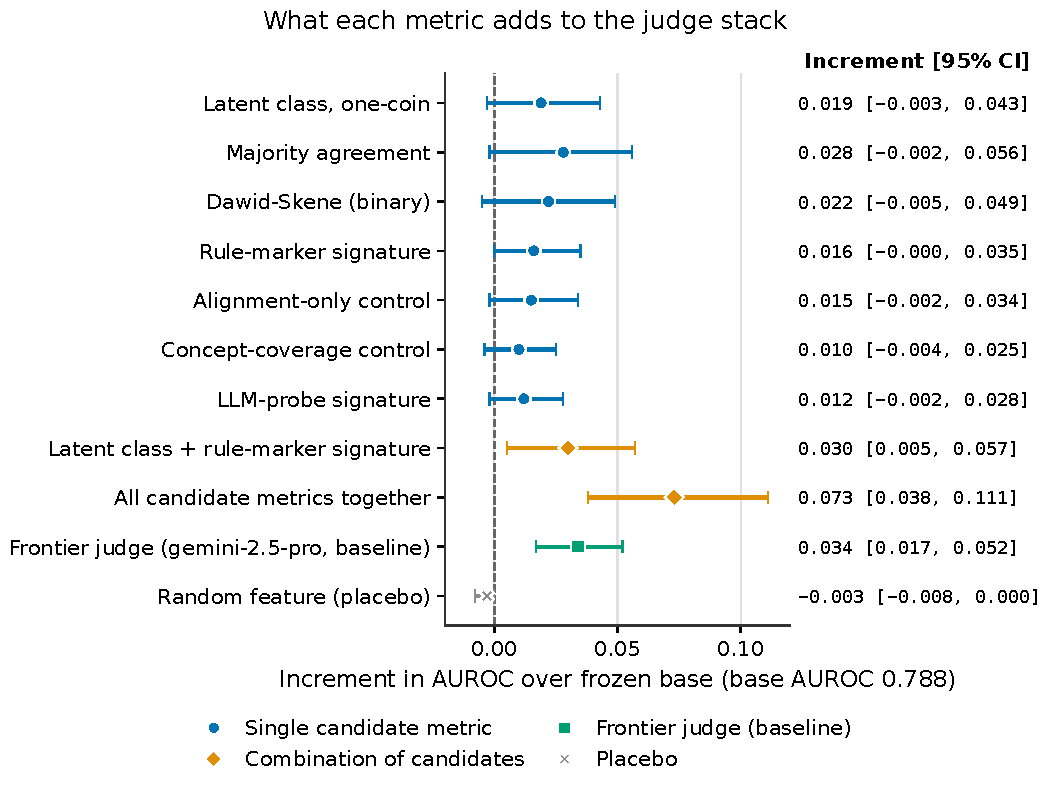
\includegraphics[width=\linewidth,height=0.85\textheight,keepaspectratio]{figures/figR4_v0.pdf}
\caption{Held-out confirmation (609 panel-adjudicated candidates, post-stratified weights): increment in cross-fitted AUROC when each metric is added to the frozen base [whole-formula judge, parse rate, round-trip NLI, round-trip cosine, structural metrics] (base AUROC 0.788), with sentence-clustered 95\% CIs. Only the frontier judge, a baseline, and combinations of candidates have a lower bound above zero; no single candidate metric does.}
\label{fig:figR4}
\end{figure}

On the 138 panel items from the two systems with samples, the base was extended with self-consistency (AUROC 0.838). Self-consistency itself adds +0.026 [$-$0.008, 0.067] to the frozen base there, and nothing else adds to the extended base: latent class $-$0.026, latent class within one system $-$0.004, rule-marker $-$0.008, LLM probe $-$0.009, predicate-set Jaccard +0.003, all with CIs spanning zero. On the same 138 items, latent class within one system (0.728) is below latent class across nine systems (0.744); under solver labels on 1,299 items the gap is 0.753 against 0.815. System diversity carries part of the latent-class signal.

\subsubsection{Is latent class a checker artefact?}

The pre-registered circularity test restricts the panel items to the 545 whose candidate the solver calls non-equivalent to the audited gold. Solver labels call all of them wrong; the panel judged 43.9\% faithful. A metric that only reproduces the equivalence checker has nothing to separate inside this subset. Table 130 shows that latent-class agreement still separates them at 0.722, so its pre-registered reading is ``not a checker artefact''. Its AUROC against panel labels does not differ significantly from its AUROC against solver labels on the same items ($-$0.042 [$-$0.110, 0.018]). The judges gain under panel labels instead: the frontier judge by +0.089.

The class positions give the same picture from another side. Panel-faithful candidates that the solver calls non-equivalent sit in a minority or singleton latent class 35\% of the time (mean score 0.58); panel-unfaithful non-equivalent candidates do so 69\% of the time (mean score 0.26).

{\small
\setlength{\tabcolsep}{3pt}
\begin{longtable}{>{\raggedright\arraybackslash}p{0.283\linewidth}>{\raggedright\arraybackslash}p{0.288\linewidth}>{\raggedright\arraybackslash}p{0.205\linewidth}>{\raggedright\arraybackslash}p{0.163\linewidth}}
\caption*{\textbf{Table 130.} Circularity test on panel items. (b) AUROC within the 545 solver-non-equivalent items; (d) within the subset where no predicate bijection to gold exists; (a) AUROC against panel labels minus AUROC against solver labels on the same items. \textit{[Source: the earlier run's round-2 frozen held-out confirmation artifact (earlier run, iteration 2)]}}\\
\toprule
\textbf{Metric} & \textbf{(b) non-equivalent only [CI]} & \textbf{(d) no bijection [CI]} & \textbf{(a) panel $-$ solver [CI]} \\
\midrule
\endfirsthead
\multicolumn{4}{l}{\textit{(continued)}}\\
\toprule
\textbf{Metric} & \textbf{(b) non-equivalent only [CI]} & \textbf{(d) no bijection [CI]} & \textbf{(a) panel $-$ solver [CI]} \\
\midrule
\endhead
\bottomrule
\endlastfoot
{}latent class, one-coin & 0.722 [0.669, 0.770] & 0.711 [0.653, 0.767] & $-$0.042 [$-$0.110, 0.018] \\
{}majority agreement & 0.741 [0.693, 0.786] & 0.749 [0.701, 0.796] & $-$0.036 [$-$0.109, 0.027] \\
{}Dawid-Skene (binary) & 0.773 [0.729, 0.815] & 0.779 [0.734, 0.822] & $-$0.025 [$-$0.096, 0.040] \\
{}latent class, Hui-Walter & 0.721 [0.669, 0.770] & 0.711 [0.652, 0.767] & $-$0.042 [$-$0.110, 0.018] \\
{}one-coin, granularity merges & 0.726 [0.674, 0.773] & 0.715 [0.659, 0.769] & $-$0.029 [$-$0.091, 0.032] \\
{}rule-marker signature & 0.609 [0.554, 0.667] & 0.616 [0.558, 0.675] & +0.040 [$-$0.028, 0.103] \\
{}alignment-only control & 0.593 [0.536, 0.646] & 0.606 [0.544, 0.667] & $-$0.029 [$-$0.089, 0.025] \\
{}concept-coverage control & 0.602 [0.547, 0.652] & 0.618 [0.560, 0.675] & $-$0.017 [$-$0.073, 0.038] \\
{}LLM-probe signature & 0.622 [0.569, 0.676] & 0.617 [0.560, 0.677] & +0.024 [$-$0.035, 0.079] \\
{}whole-formula judge & 0.709 [0.661, 0.753] & 0.702 [0.645, 0.755] & +0.005 [$-$0.046, 0.058] \\
{}frontier judge & 0.785 [0.742, 0.823] & 0.783 [0.735, 0.826] & +0.089 [0.035, 0.142] \\
{}round-trip NLI & 0.709 [0.655, 0.757] & 0.717 [0.657, 0.769] & +0.063 [$-$0.008, 0.139] \\
{}round-trip cosine & 0.679 [0.627, 0.730] & 0.678 [0.613, 0.735] & +0.081 [0.013, 0.144] \\
{}LLM-probe signature (L) & 0.538 [0.482, 0.595] & 0.538 [0.482, 0.598] & $-$0.018 [$-$0.074, 0.040] \\
{}whole-formula judge (L) & 0.663 [0.619, 0.706] & 0.659 [0.611, 0.706] & +0.068 [0.019, 0.123] \\
{}thinking judge (L) & 0.789 [0.756, 0.824] & 0.788 [0.750, 0.823] & +0.108 [0.066, 0.153] \\
{}round-trip NLI (L) & 0.731 [0.678, 0.778] & 0.738 [0.688, 0.789] & +0.086 [0.009, 0.166] \\
{}round-trip cosine (L) & 0.670 [0.616, 0.718] & 0.688 [0.631, 0.738] & +0.046 [$-$0.018, 0.109] \\
{}round-trip LLM comparison (L) & 0.603 [0.565, 0.641] & 0.611 [0.573, 0.651] & +0.038 [0.003, 0.081] \\
{}structural (user pilot) & 0.507 [0.494, 0.524] & 0.507 [0.491, 0.527] & $-$0.004 [$-$0.013, 0.005] \\
\end{longtable}
}

\subsubsection{Complexity: no crossover for any metric}

The crossover was pre-registered as a slope across terciles in the metric-minus-judge AUROC gap, with a positive top-tercile gap. No metric met it under any labelling (Table 131). On the panel's top tercile (389 items) the cheap judge reached 0.779, above latent class at 0.719. The judge did not collapse on complex held-out items the way it did on the FOLIO screen. Only the frontier judge has a top-tercile gap over the cheap judge that excludes zero, and even it shows no slope.

{\small
\setlength{\tabcolsep}{3pt}
\begin{longtable}{>{\raggedright\arraybackslash}p{0.229\linewidth}>{\raggedright\arraybackslash}p{0.185\linewidth}>{\raggedright\arraybackslash}p{0.184\linewidth}>{\raggedright\arraybackslash}p{0.160\linewidth}>{\raggedright\arraybackslash}p{0.167\linewidth}}
\caption*{\textbf{Table 131.} Pre-registered crossover test: metric $-$ whole-formula judge AUROC gap per tercile, with slope and top-tercile gap CIs, under panel (P), audited-solver (S) and soft (T) labels. \textit{[Source: the earlier run's round-2 frozen held-out confirmation artifact (earlier run, iteration 2)]}}\\
\toprule
\textbf{Labels $\cdot$ metric} & \textbf{gap bottom / middle / top} & \textbf{slope [CI]} & \textbf{top gap CI} & \textbf{crossover} \\
\midrule
\endfirsthead
\multicolumn{5}{l}{\textit{(continued)}}\\
\toprule
\textbf{Labels $\cdot$ metric} & \textbf{gap bottom / middle / top} & \textbf{slope [CI]} & \textbf{top gap CI} & \textbf{crossover} \\
\midrule
\endhead
\bottomrule
\endlastfoot
{}P $\cdot$ latent class & $-$0.051 / +0.136 / $-$0.059 & $-$0.004 [$-$0.074, 0.064] & [$-$0.137, 0.015] & no \\
{}P $\cdot$ rule-marker signature & $-$0.144 / +0.038 / $-$0.209 & $-$0.032 [$-$0.117, 0.055] & [$-$0.307, $-$0.108] & no \\
{}P $\cdot$ LLM-probe signature & $-$0.114 / +0.011 / $-$0.183 & $-$0.034 [$-$0.114, 0.040] & [$-$0.279, $-$0.089] & no \\
{}P $\cdot$ frontier judge & $-$0.004 / +0.143 / +0.056 & +0.030 [$-$0.031, 0.088] & [0.008, 0.109] & no \\
{}P $\cdot$ round-trip NLI & $-$0.074 / +0.128 / $-$0.110 & $-$0.018 [$-$0.090, 0.055] & [$-$0.192, $-$0.029] & no \\
{}S $\cdot$ latent class & +0.129 / +0.103 / +0.071 & $-$0.029 [$-$0.059, 0.005] & [0.032, 0.106] & no \\
{}S $\cdot$ rule-marker signature & $-$0.108 / $-$0.107 / $-$0.130 & $-$0.011 [$-$0.052, 0.030] & [$-$0.184, $-$0.079] & no \\
{}S $\cdot$ LLM-probe signature & $-$0.068 / $-$0.079 / $-$0.167 & $-$0.050 [$-$0.096, 0.003] & [$-$0.215, $-$0.114] & no \\
{}S $\cdot$ frontier judge & +0.020 / +0.136 / +0.050 & +0.015 [$-$0.040, 0.068] & [0.005, 0.091] & no \\
{}S $\cdot$ round-trip NLI & $-$0.029 / +0.014 / $-$0.068 & $-$0.020 [$-$0.071, 0.035] & [$-$0.140, 0.005] & no \\
{}T $\cdot$ latent class & +0.077 / +0.040 / +0.023 & $-$0.027 [$-$0.046, $-$0.009] & [0.003, 0.043] & no \\
{}T $\cdot$ rule-marker signature & $-$0.080 / $-$0.036 / $-$0.028 & +0.026 [$-$0.000, 0.050] & [$-$0.053, $-$0.001] & no \\
{}T $\cdot$ LLM-probe signature & $-$0.079 / +0.010 / $-$0.046 & +0.017 [$-$0.018, 0.047] & [$-$0.071, $-$0.017] & no \\
{}T $\cdot$ frontier judge & +0.020 / +0.136 / +0.050 & +0.015 [$-$0.036, 0.062] & [0.005, 0.093] & no \\
{}T $\cdot$ round-trip NLI & $-$0.026 / +0.066 / $-$0.059 & $-$0.016 [$-$0.059, 0.031] & [$-$0.112, $-$0.004] & no \\
\end{longtable}
}

Table 132 breaks the panel and solver-labelled populations down by tercile and by the number of conditions. Under solver labels the Dawid-Skene form of latent class is best in every cell except four or more conditions, where the frontier judge edges it (0.877 against 0.866). Under panel labels the frontier judge or the Dawid-Skene form leads every cell except the bottom tercile, where the cheap judge does (0.798). Latent class beats the cheap judge in the middle tercile and on 0-1 and 4+ conditions, and trails it in the bottom and top terciles and on 2-3 conditions; nothing in the pattern grows with complexity.

{\footnotesize
\setlength{\tabcolsep}{3pt}
\begin{longtable}{>{\raggedright\arraybackslash}p{0.057\linewidth}>{\raggedright\arraybackslash}p{0.124\linewidth}>{\raggedright\arraybackslash}p{0.084\linewidth}>{\raggedright\arraybackslash}p{0.151\linewidth}>{\raggedright\arraybackslash}p{0.151\linewidth}>{\raggedright\arraybackslash}p{0.071\linewidth}>{\raggedright\arraybackslash}p{0.111\linewidth}>{\raggedright\arraybackslash}p{0.138\linewidth}}
\caption*{\textbf{Table 132.} AUROC per complexity cell. tn = tercile (1 bottom, 3 top); nbin = number of conditions. n gives items (faithful / unfaithful). \textit{[Source: the earlier run's round-2 frozen held-out confirmation artifact (earlier run, iteration 2)]}}\\
\toprule
\textbf{Cell} & \textbf{n (pos/neg)} & \textbf{latent class} & \textbf{Dawid-Skene} & \textbf{rule-marker} & \textbf{judge} & \textbf{frontier judge} & \textbf{round-trip NLI} \\
\midrule
\endfirsthead
\multicolumn{8}{l}{\textit{(continued)}}\\
\toprule
\textbf{Cell} & \textbf{n (pos/neg)} & \textbf{latent class} & \textbf{Dawid-Skene} & \textbf{rule-marker} & \textbf{judge} & \textbf{frontier judge} & \textbf{round-trip NLI} \\
\midrule
\endhead
\bottomrule
\endlastfoot
{}P $\cdot$ tn=1 & 105 (64/41) & 0.747 & 0.754 & 0.654 & 0.798 & 0.794 & 0.724 \\
{}P $\cdot$ tn=2 & 115 (67/48) & 0.808 & 0.825 & 0.709 & 0.671 & 0.814 & 0.799 \\
{}P $\cdot$ tn=3 & 389 (176/213) & 0.719 & 0.777 & 0.570 & 0.779 & 0.834 & 0.668 \\
{}P $\cdot$ nbin 0-1 & 209 (116/93) & 0.793 & 0.810 & 0.659 & 0.741 & 0.796 & 0.765 \\
{}P $\cdot$ nbin 2-3 & 241 (119/122) & 0.653 & 0.708 & 0.626 & 0.753 & 0.804 & 0.674 \\
{}P $\cdot$ nbin 4+ & 159 (72/87) & 0.857 & 0.874 & 0.657 & 0.800 & 0.909 & 0.768 \\
{}S $\cdot$ tn=1 & 1528 (729/799) & 0.841 & 0.876 & 0.605 & 0.713 & 0.800 & 0.656 \\
{}S $\cdot$ tn=2 & 1773 (666/1107) & 0.794 & 0.808 & 0.583 & 0.691 & 0.794 & 0.623 \\
{}S $\cdot$ tn=3 & 2546 (822/1724) & 0.790 & 0.808 & 0.589 & 0.719 & 0.787 & 0.619 \\
{}S $\cdot$ nbin 0-1 & 2363 (877/1486) & 0.813 & 0.847 & 0.602 & 0.707 & 0.773 & 0.619 \\
{}S $\cdot$ nbin 2-3 & 2093 (738/1355) & 0.770 & 0.796 & 0.583 & 0.668 & 0.775 & 0.599 \\
{}S $\cdot$ nbin 4+ & 1391 (602/789) & 0.865 & 0.866 & 0.677 & 0.774 & 0.877 & 0.689 \\
\end{longtable}
}

\subsubsection{Detection by real error type}

The panel's adjudicated primary error type makes it possible to ask which real errors each metric catches: the AUROC between panel-faithful items and the unfaithful items of one type (Table 133). Latent class is strongest on $\forall$/$\exists$ and implication-direction errors. The rule-marker signature does best on implication direction (0.825) and is at chance on $\forall$/$\exists$ (0.529), the second most common real error. The frontier judge leads on most types. On the 16 quantifier-scope errors the cheap judge (0.847) is best, and every metric except the structural one sees them above chance, including the signature (0.633), which was predicted to be blind to them.

\begin{landscape}
{\footnotesize
\setlength{\tabcolsep}{3pt}
\begin{longtable}{>{\raggedright\arraybackslash}p{0.072\linewidth}>{\raggedright\arraybackslash}p{0.015\linewidth}>{\raggedright\arraybackslash}p{0.052\linewidth}>{\raggedright\arraybackslash}p{0.092\linewidth}>{\raggedright\arraybackslash}p{0.092\linewidth}>{\raggedright\arraybackslash}p{0.076\linewidth}>{\raggedright\arraybackslash}p{0.116\linewidth}>{\raggedright\arraybackslash}p{0.044\linewidth}>{\raggedright\arraybackslash}p{0.068\linewidth}>{\raggedright\arraybackslash}p{0.084\linewidth}>{\raggedright\arraybackslash}p{0.084\linewidth}>{\raggedright\arraybackslash}p{0.084\linewidth}}
\caption*{\textbf{Table 133.} AUROC of faithful panel items against the unfaithful items of one primary error type (n unfaithful in the second column; panel items, weighted). \textit{[Source: the earlier run's round-2 frozen held-out confirmation artifact (earlier run, iteration 2)]}}\\
\toprule
\textbf{Error type} & \textbf{n} & \textbf{latent class} & \textbf{Dawid-Skene} & \textbf{rule-marker} & \textbf{LLM-probe sig.} & \textbf{alignment-only} & \textbf{judge} & \textbf{frontier judge} & \textbf{round-trip NLI} & \textbf{round-trip cosine} & \textbf{structural} \\
\midrule
\endfirsthead
\multicolumn{12}{l}{\textit{(continued)}}\\
\toprule
\textbf{Error type} & \textbf{n} & \textbf{latent class} & \textbf{Dawid-Skene} & \textbf{rule-marker} & \textbf{LLM-probe sig.} & \textbf{alignment-only} & \textbf{judge} & \textbf{frontier judge} & \textbf{round-trip NLI} & \textbf{round-trip cosine} & \textbf{structural} \\
\midrule
\endhead
\bottomrule
\endlastfoot
{}added condition & 74 & 0.701 & 0.726 & 0.680 & 0.657 & 0.628 & 0.731 & 0.803 & 0.727 & 0.745 & 0.505 \\
{}$\forall$/$\exists$ choice & 60 & 0.842 & 0.831 & 0.529 & 0.598 & 0.594 & 0.789 & 0.853 & 0.737 & 0.732 & 0.517 \\
{}dropped condition & 47 & 0.756 & 0.823 & 0.634 & 0.704 & 0.757 & 0.667 & 0.737 & 0.785 & 0.746 & 0.510 \\
{}implication direction / ``only'' & 29 & 0.837 & 0.873 & 0.825 & 0.769 & 0.662 & 0.768 & 0.846 & 0.732 & 0.764 & 0.526 \\
{}syntax / unparseable & 17 & 0.707 & 0.759 & 0.704 & 0.756 & 0.656 & 0.921 & 0.931 & 0.837 & 0.773 & 0.495 \\
{}quantifier scope & 16 & 0.704 & 0.736 & 0.633 & 0.594 & 0.566 & 0.847 & 0.775 & 0.665 & 0.672 & 0.495 \\
{}conflation & 16 & 0.724 & 0.813 & 0.675 & 0.705 & 0.767 & 0.781 & 0.892 & 0.760 & 0.626 & 0.520 \\
{}conjunction / disjunction & 14 & 0.881 & 0.932 & 0.767 & 0.779 & 0.642 & 0.900 & 0.964 & 0.849 & 0.789 & 0.495 \\
{}negation / polarity & 10 & 0.727 & 0.764 & 0.755 & 0.791 & 0.800 & 0.930 & 0.914 & 0.833 & 0.693 & 0.581 \\
\end{longtable}
}
\end{landscape}

\subsubsection{System level}

System-level Kendall $\tau$ was computed against a post-stratified per-system faithfulness rate (Table 134). With nine systems whose true rates span 0.46 (llama-3.1-8b) to 0.65 (gpt-oss-120b), $\tau$ is easy on all items: the cheap judge reaches 0.889 and even parse rate 0.817. Against panel-only system accuracies the CIs are wide. The random metric sits at $-$0.278.

{\small
\setlength{\tabcolsep}{3pt}
\begin{longtable}{>{\raggedright\arraybackslash}p{0.303\linewidth}>{\raggedright\arraybackslash}p{0.221\linewidth}>{\raggedright\arraybackslash}p{0.194\linewidth}>{\raggedright\arraybackslash}p{0.221\linewidth}}
\caption*{\textbf{Table 134.} System-level Kendall $\tau$\_\allowbreak{}b over nine systems [bootstrap CI over sentences]. \textit{[Source: the earlier run's round-2 frozen held-out confirmation artifact (earlier run, iteration 2)]}}\\
\toprule
\textbf{Metric} & \textbf{$\tau$\_\allowbreak{}b, all items} & \textbf{pairwise order accuracy} & \textbf{$\tau$\_\allowbreak{}b, panel items} \\
\midrule
\endfirsthead
\multicolumn{4}{l}{\textit{(continued)}}\\
\toprule
\textbf{Metric} & \textbf{$\tau$\_\allowbreak{}b, all items} & \textbf{pairwise order accuracy} & \textbf{$\tau$\_\allowbreak{}b, panel items} \\
\midrule
\endhead
\bottomrule
\endlastfoot
{}latent class, one-coin & 0.778 [0.667, 0.944] & 0.889 & 0.556 [0.111, 0.778] \\
{}majority agreement & 0.722 [0.556, 0.833] & 0.861 & 0.278 [$-$0.111, 0.667] \\
{}Dawid-Skene (binary) & 0.722 [0.611, 0.889] & 0.861 & 0.278 [$-$0.167, 0.667] \\
{}rule-marker signature & 0.833 [0.667, 0.889] & 0.917 & 0.222 [$-$0.056, 0.667] \\
{}alignment-only control & 0.556 [0.389, 0.722] & 0.778 & 0.333 [0.056, 0.722] \\
{}LLM-probe signature & n/a & n/a & 0.333 [$-$0.056, 0.667] \\
{}whole-formula judge & 0.889 [0.722, 0.944] & 0.944 & 0.722 [0.389, 0.889] \\
{}frontier judge & n/a & n/a & 0.778 [0.444, 0.944] \\
{}round-trip NLI & n/a & n/a & 0.722 [0.333, 0.833] \\
{}whole-formula judge (L) & 0.889 [0.778, 1.000] & 0.944 & 0.333 [0.165, 0.722] \\
{}thinking judge (L) & n/a & n/a & 0.778 [0.444, 0.889] \\
{}parse rate & 0.817 [0.592, 0.889] & 0.889 & n/a \\
{}structural (user pilot) & 0.761 [0.500, 0.833] & 0.861 & 0.377 [$-$0.131, 0.609] \\
{}random & $-$0.278 [$-$0.611, 0.111] & 0.361 & $-$0.056 [$-$0.389, 0.333] \\
\end{longtable}
}

The post-stratified faithfulness rates used as truth were gpt-oss-120b 0.649, gpt-4.1-mini 0.639, gemini-2.5-flash 0.635, gemma-3-27b 0.591, deepseek-v3.1 0.572, mistral-small-3.2 0.552, phi-4 0.506, qwen-2.5-7b 0.475 and llama-3.1-8b 0.463.

\subsubsection{Contamination}

Public benchmarks can leak into the training data of the models that judge them [39]. The contamination group pairs 104 verified sentences with entity-renamed paraphrases, each formalized by the nine systems (936 rows). Every metric scored the originals higher than the paraphrases, and no metric's AUROC changed significantly between the two (Table 135). For the zero-LLM signature metrics the score drop comes from the lexical aligner, which breaks under renamed entities. The local gold-recall probe recalled 0.335 of gold predicate names on originals and 0.243 on paraphrases (+0.092 [0.014, 0.169]); exact gold recall was about 1\% on both. That is mild familiarity with gold vocabulary and no verbatim recall. The gemini recall probe was not run. A self-preference check [38] found the frontier judge at 0.853 on the two Google-family generators and 0.817 on the others (130 own-family items).

{\small
\setlength{\tabcolsep}{3pt}
\begin{longtable}{>{\raggedright\arraybackslash}p{0.330\linewidth}>{\raggedright\arraybackslash}p{0.181\linewidth}>{\raggedright\arraybackslash}p{0.108\linewidth}>{\raggedright\arraybackslash}p{0.108\linewidth}>{\raggedright\arraybackslash}p{0.198\linewidth}}
\caption*{\textbf{Table 135.} Original vs entity-renamed paraphrase (936 rows, 104 sentence pairs). \textit{[Source: the earlier run's round-2 frozen held-out confirmation artifact (earlier run, iteration 2)]}}\\
\toprule
\textbf{Metric} & \textbf{mean score $\Delta$ (orig $-$ para) [CI]} & \textbf{AUROC orig} & \textbf{AUROC para} & \textbf{AUROC diff [CI]} \\
\midrule
\endfirsthead
\multicolumn{5}{l}{\textit{(continued)}}\\
\toprule
\textbf{Metric} & \textbf{mean score $\Delta$ (orig $-$ para) [CI]} & \textbf{AUROC orig} & \textbf{AUROC para} & \textbf{AUROC diff [CI]} \\
\midrule
\endhead
\bottomrule
\endlastfoot
{}whole-formula judge & +0.096 [0.068, 0.126] & 0.625 & 0.647 & $-$0.022 [$-$0.067, 0.030] \\
{}round-trip cosine & +0.070 [0.029, 0.107] & 0.626 & 0.601 & +0.025 [$-$0.031, 0.088] \\
{}round-trip NLI & +0.074 [0.018, 0.131] & 0.611 & 0.565 & +0.046 [$-$0.034, 0.129] \\
{}LLM-probe signature & +0.142 [0.112, 0.176] & 0.564 & 0.532 & +0.032 [$-$0.055, 0.121] \\
{}whole-formula judge (L) & +0.026 [0.013, 0.039] & 0.577 & 0.608 & $-$0.032 [$-$0.068, 0.010] \\
{}round-trip cosine (L) & +0.101 [0.071, 0.130] & 0.516 & 0.554 & $-$0.038 [$-$0.125, 0.052] \\
{}round-trip NLI (L) & +0.092 [0.035, 0.150] & 0.584 & 0.543 & +0.042 [$-$0.029, 0.117] \\
{}round-trip LLM comparison (L) & +0.119 [0.064, 0.179] & 0.532 & 0.551 & $-$0.018 [$-$0.073, 0.039] \\
{}LLM-probe signature (L) & +0.106 [0.078, 0.137] & 0.581 & 0.510 & +0.072 [$-$0.016, 0.164] \\
{}rule-marker signature & +0.141 [0.108, 0.175] & 0.579 & 0.525 & +0.054 [$-$0.052, 0.158] \\
{}alignment-only control & +0.186 [0.158, 0.214] & 0.559 & 0.529 & +0.030 [$-$0.062, 0.126] \\
{}concept-coverage control & +0.236 [0.201, 0.275] & 0.567 & 0.598 & $-$0.031 [$-$0.094, 0.035] \\
\end{longtable}
}

\subsubsection{Judge reliability}

The cheap judge was re-asked 300 times sequentially. Test-retest Spearman was 0.965, 91.3\% of scores were identical and 2.3\% moved by more than 0.2. Its prompts are 19\% duplicates, and it produces only 12 distinct scores. The local substitute was steadier (Spearman 0.974) but weaker.

\subsubsection{The screen re-ranked under audited labels}

Iteration 1 pre-registered that its selection rule would be re-applied with the dataset's audited screen labels, and that the audited ranking would govern. The artifact joined both arms' screen scores to the audited labels by normalized sentence and system (832 of 835 Arm A items, 830 of 833 Arm B items), excluded the stories whose premise lists Arm A had misaligned, and re-ran each arm's own gate code (Table 136). The outcome did not change: latent-class agreement is still the only survivor and the winner, and no signature variant survives. Under audited labels the signature variants rise sharply, the rule-marker signature from 0.713 to 0.772 overall and from 0.50 to 0.72 in the top tercile. They still fail the false-alarm gate, whose value is carried over from iteration 1. The audited labels are still solver equivalence, so this re-rank cannot test the circularity; only the held-out tests above do.

\begin{table}[H]
\centering
\scriptsize
\setlength{\tabcolsep}{3pt}
\caption*{\textbf{Table 136.} Screen re-rank: iteration-1 labels vs audited labels (Arm A n = 754, 78\% label agreement; Arm B n = 763, 85\% label agreement). Gates: coverage / false alarms / increment / floor. \textit{[Source: the earlier run's round-2 frozen held-out confirmation artifact (earlier run, iteration 2)]}}
\begin{tabular}{>{\raggedright\arraybackslash}p{0.171\linewidth}>{\raggedright\arraybackslash}p{0.069\linewidth}>{\raggedright\arraybackslash}p{0.080\linewidth}>{\raggedright\arraybackslash}p{0.102\linewidth}>{\raggedright\arraybackslash}p{0.080\linewidth}>{\raggedright\arraybackslash}p{0.080\linewidth}>{\raggedright\arraybackslash}p{0.102\linewidth}>{\raggedright\arraybackslash}p{0.102\linewidth}>{\raggedright\arraybackslash}p{0.091\linewidth}}
\toprule
\textbf{Arm $\cdot$ metric} & \textbf{AUROC iter-1 labels} & \textbf{top tercile} & \textbf{increment [CI]} & \textbf{AUROC audited labels} & \textbf{top tercile} & \textbf{increment [CI]} & \textbf{gates failed (audited)} & \textbf{survives} \\
\midrule
{}A $\cdot$ LLM-probe signature & 0.699 & 0.487 & +0.095 [0.043, 0.146] & 0.769 & 0.688 & +0.095 [0.050, 0.139] & false alarms & no \\
{}A $\cdot$ relativized signature & 0.698 & 0.488 & +0.094 [0.042, 0.145] & 0.769 & 0.688 & +0.094 [0.049, 0.139] & false alarms & no \\
{}A $\cdot$ rule-marker signature & 0.713 & 0.499 & +0.113 [0.058, 0.163] & 0.772 & 0.715 & +0.098 [0.053, 0.149] & false alarms & no \\
{}A $\cdot$ alignment-only control & 0.654 & 0.499 & +0.066 [0.019, 0.109] & 0.711 & 0.664 & +0.073 [0.036, 0.113] & false alarms & no \\
{}A $\cdot$ concept-coverage control & 0.647 & 0.447 & +0.068 [0.020, 0.110] & 0.705 & 0.656 & +0.059 [0.021, 0.100] & false alarms & no \\
{}B $\cdot$ truth-value-judgment worlds & 0.697 & 0.738 & +0.056 [0.025, 0.085] & 0.697 & 0.664 & +0.029 [0.001, 0.055] & false alarms & no \\
{}B $\cdot$ instance NLI (DeBERTa) & 0.583 & 0.478 & $-$0.005 [$-$0.020, 0.010] & 0.615 & 0.527 & $-$0.000 [$-$0.023, 0.021] & false alarms, increment, floor & no \\
{}B $\cdot$ latent class, one-coin & 0.844 & 0.822 & +0.138 [0.096, 0.179] & 0.809 & 0.814 & +0.080 [0.044, 0.115] & none & \textbf{yes} \\
\bottomrule
\end{tabular}
\end{table}

Under audited labels the truth-value-judgment worlds lose their top-tercile advantage (0.738 to 0.664), a first sign of what round 2, part 3 found on held-out data.

\subsubsection{Transfer to the user's pilot}

Latent class cannot run on the EU-AI-Act pilot, which has one system per definition. The rule-marker signature covered 71\% of the 367 formulas (262 scored). The uncovered ones are the \texttt{$\subseteq$}, \texttt{$\Rightarrow$} and quote symbols that do not parse (counted), plus low alignment coverage. Its predicted type was ``conflation'' for 98\% of the covered formulas. The iteration-1 error-type rules are degenerate on definitional text: on held-out panel-unfaithful items they also predict conflation 54\% of the time, while the panel's real mix is led by added conditions (25\%) and $\forall$/$\exists$ (22\%). No accuracy claim is possible here.

\subsubsection{Reproduction}

An independent numpy re-derivation matched the panel AUROCs of latent class (0.7555), rule-marker signature (0.6418) and whole-formula judge (0.7621), and the circularity AUROCs (0.7224, 0.6094, 0.7088), to within 1e-6. An independent logistic stack gave a latent-class increment of +0.020 against the analysis value of +0.019. Permuted labels gave mean AUROC 0.50; a random metric scored 0.512 [0.456, 0.566]. For this report we joined the per-item score file to the dataset's panel labels once more (\texttt{checks/\allowbreak{}recompute\_\allowbreak{}\allowbreak{}iter2.py}) and reproduced every panel AUROC in Table 128 that we checked to three decimals, except the LLM-probe signature (0.659 against 0.657), whose uncovered rows the artifact handles slightly differently.

\subsection{Round 2, part 3: Truth-value-judgment worlds: repair, freeze and the crossover test}

\subsubsection{Phase 1: repair on the screen only}

The plan attributed the iteration-1 false alarms to three sources, and the artifact built one repair for each. Worlds are now computed from a canonical, name-blind normal form of the formula: negation normal form with parity handling for $\leftrightarrow$ and $\oplus$, a single normal form for A $\rightarrow$ B, $\neg$B $\rightarrow$ $\neg$A and $\neg$A $\vee$ B, operands sorted without reference to names, alpha-renamed variables and prenexing. Every canonical form was verified bounded-equivalent to its source, with 0 fallbacks on the 300 screen golds. Mutants are generated from the canonical form with a name-blind seed, and z3 [13] minimal distinguishing worlds are deduplicated by isomorphism. Judge noise is handled by a world-level answer cache keyed by the verbalized world, three votes over fixed world orders, and a prompt that returns a verdict with a confidence. The frozen score is the confidence-weighted agreement.

The world-set diagnostic in Table 137 shows the canonical form doing what it was built to do. Equivalent reorder, De Morgan and contrapositive rewrites now receive exactly the gold's world set; in iteration 1 they received it between 2\% and 18\% of the time. On the held-out set the same held for 137 of 137 non-renaming rewrites, including their verbalizations, and for 59 of 60 renamings.

\begin{table}[H]
\centering
\small
\setlength{\tabcolsep}{3pt}
\caption*{\textbf{Table 137.} Share of solver-verified equivalent rewrites of the 300 screen golds whose world set is identical to the gold's. \textit{[Source: the earlier run's round-2 truth-value-judgment deep-test artifact (earlier run, iteration 2)]}}
\begin{tabular}{>{\raggedright\arraybackslash}p{0.416\linewidth}>{\raggedright\arraybackslash}p{0.069\linewidth}>{\raggedright\arraybackslash}p{0.247\linewidth}>{\raggedright\arraybackslash}p{0.207\linewidth}}
\toprule
\textbf{Rewrite kind} & \textbf{n} & \textbf{iteration-1 worlds} & \textbf{canonical worlds} \\
\midrule
{}reorder & 66 & 0.182 & 1.000 \\
{}De Morgan & 55 & 0.018 & 1.000 \\
{}contrapositive & 104 & 0.125 & 1.000 \\
{}predicate renaming (up to renaming) & 274 & 0.628 & 0.996 \\
\bottomrule
\end{tabular}
\end{table}

A zero-cost analysis of the iteration-1 cached answers located the old false alarms. gemini-2.5-flash at temperature 0 gave different verdicts to the same sentence and the same verbalized world in 13.7\% of the 1,186 cases where that pair appeared in two or more prompts. Non-renaming false alarms occurred only when a rewrite's world set had changed: on the 26 non-renaming rewrites whose iteration-1 world set matched the gold's, the paired false-alarm rate was 0. Renamings kept a 0.34 rate even with identical worlds, which points at the verbalizer.

While testing, the artifact found a bug in the iteration-1 world finder. It tagged every z3 grounder with a global counter, and z3's main context carried solver state across calls, so the choice among equally minimal worlds depended on call history: the same formula could receive different worlds. A unit test caught it. The fix, a fixed tag and a fresh z3 context per call, changed 57 of 1,039 screen world sets and raised renaming identity from 0.971 to 0.996 on the screen and from 0.817 to 0.983 on held-out. The iteration-1 worlds were affected by the same non-determinism. A second bug, a cache alias that could shadow a world record, affected 9 held-out items, which were re-scored at no cost.

Table 138 gives the repaired protocol judged by gemini on the screen. The canonical worlds remove every non-renaming false alarm. Renaming alarms stay at 0.37 to 0.39. Screen AUROC rises from 0.701 to 0.735, and the confidence-weighted score is 0.069 above the iteration-1 judge. Test-retest agreement on 141 items (351 worlds) was $\kappa$ = 0.94 at the world level and ICC(2,1) = 0.96 for the single-vote score. Malformed JSON occurred in 0.1\% of answers. The repair phase cost \$0.54.

\begin{table}[H]
\centering
\footnotesize
\setlength{\tabcolsep}{3pt}
\caption*{\textbf{Table 138.} Repaired protocol on the screen (833 real candidates, Arm B labels). Single vote = binary verdict of one call; majority = 3-vote majority; confidence-weighted = the frozen score. Paired false alarm = rewrite score more than 0.2 below its gold's score. Iteration-1 paired values come from the zero-cost decomposition. \textit{[Source: the earlier run's round-2 truth-value-judgment deep-test artifact (earlier run, iteration 2)]}}
\begin{tabular}{>{\raggedright\arraybackslash}p{0.136\linewidth}>{\raggedright\arraybackslash}p{0.090\linewidth}>{\raggedright\arraybackslash}p{0.118\linewidth}>{\raggedright\arraybackslash}p{0.246\linewidth}>{\raggedright\arraybackslash}p{0.161\linewidth}>{\raggedright\arraybackslash}p{0.161\linewidth}}
\toprule
\textbf{} & \textbf{single vote} & \textbf{majority} & \textbf{confidence-weighted (frozen)} & \textbf{iteration-1 worlds} & \textbf{iteration-1 judge} \\
\midrule
{}AUROC on real candidates & 0.698 & 0.684 & 0.735 [0.686, 0.778] & 0.701 & 0.666 \\
{}paired false alarms, non-renaming rewrites (n = 225) & 0.000 & 0.000 & 0.000 & 0.102 & n/a \\
{}paired false alarms, renaming (n = 274) & 0.376 & 0.369 & 0.387 & 0.372 & n/a \\
{}paired false alarms, all (n = 499) & 0.206 & 0.202 & 0.212 & 0.251 & n/a \\
\bottomrule
\end{tabular}
\end{table}

By rewrite kind, the iteration-1 paired false-alarm rates had been 0.030 for reorder, 0.091 for De Morgan, 0.154 for contrapositive and 0.372 for renaming.

\subsubsection{The freeze, and what the key outage did to it}

The frozen configuration and pre-registration were hashed into a receipt, and the label loader refuses to run unless the hashes match. The shared key was at its daily limit for about an hour around the planned freeze, so the screen judging that the freeze rule needed could not run before the freeze. Following the plan's fallback, the freeze used the pre-declared default, the confidence-weighted score. When the key returned, the screen was judged, and the freeze rule applied after the fact picks the same score: no configuration passes the 10\% false-alarm bar overall, all pass it on non-renaming rewrites, and that branch of the rule chooses by AUROC. Held-out labels had been loaded before the world-finder fix, but only for the zero-LLM analyses; no held-out world or judge score existed at that time. The aggregate panel label marginals (307/302) and error-type counts were printed once during setup.

\subsubsection{Phase 2: held-out results}

Three item sets were scored: the 609 panel items with post-stratified weights (389 in the top tercile, enough for the pre-registered test to run on the panel top tercile); all 2,826 top-tercile candidates with soft and solver labels; and the 936 contamination rows. The cheap judge was re-run with the exact iteration-1 prompt, and a compute-matched judge averaged three independent calls. Table 139 gives the result.

The repaired worlds lose to the cheap judge overall and in the bottom and top terciles, tie it in the middle tercile (0.657 against 0.654), and lose by more to the compute-matched judge. The repair did not add held-out discrimination: the repaired score is 0.020 below the unrepaired iteration-1 protocol on all panel items. Within a sentence, the repaired score orders a faithful and an unfaithful candidate correctly less than half the time (0.475), where the judge does so 0.758 of the time; what discrimination the worlds have separates sentences, not candidates. A flash-lite judge made the worlds nearly useless (0.565). The same ordering held on the 586 jointly covered items (worlds 0.666, judge 0.745) and on the 538 items not generated by gemini (0.655 and 0.752).

{\scriptsize
\setlength{\tabcolsep}{3pt}
\begin{longtable}{>{\raggedright\arraybackslash}p{0.128\linewidth}>{\raggedright\arraybackslash}p{0.071\linewidth}>{\raggedright\arraybackslash}p{0.078\linewidth}>{\raggedright\arraybackslash}p{0.078\linewidth}>{\raggedright\arraybackslash}p{0.071\linewidth}>{\raggedright\arraybackslash}p{0.128\linewidth}>{\raggedright\arraybackslash}p{0.066\linewidth}>{\raggedright\arraybackslash}p{0.066\linewidth}>{\raggedright\arraybackslash}p{0.190\linewidth}}
\caption*{\textbf{Table 139.} Weighted AUROC on the 609 panel items, by complexity tercile and number of conditions [95\% CI for all items and top tercile], and within-sentence pairwise accuracy (122 pairs). 2000$\times$ sentence-cluster bootstrap with corpus strata. \textit{[Source: the earlier run's round-2 truth-value-judgment deep-test artifact (earlier run, iteration 2)]}}\\
\toprule
\textbf{Metric} & \textbf{all (609)} & \textbf{bottom (105)} & \textbf{middle (115)} & \textbf{top (389)} & \textbf{conditions 0-1 (209)} & \textbf{2-3 (241)} & \textbf{4+ (159)} & \textbf{within-sentence} \\
\midrule
\endfirsthead
\multicolumn{9}{l}{\textit{(continued)}}\\
\toprule
\textbf{Metric} & \textbf{all (609)} & \textbf{bottom (105)} & \textbf{middle (115)} & \textbf{top (389)} & \textbf{conditions 0-1 (209)} & \textbf{2-3 (241)} & \textbf{4+ (159)} & \textbf{within-sentence} \\
\midrule
\endhead
\bottomrule
\endlastfoot
{}worlds, repaired (frozen, 3 votes) & 0.665 [0.607, 0.718] & 0.655 & 0.657 & 0.674 [0.597, 0.744] & 0.713 & 0.596 & 0.726 & 0.475 \\
{}worlds, repaired, single vote & 0.669 & 0.655 & 0.678 & 0.653 & 0.723 & 0.636 & 0.654 & 0.504 \\
{}worlds, iteration-1 protocol & 0.685 & 0.675 & 0.690 & 0.671 & 0.714 & 0.659 & 0.705 & 0.537 \\
{}worlds, repaired, flash-lite judge & 0.565 & 0.525 & 0.604 & 0.533 & 0.587 & 0.542 & 0.608 & 0.484 \\
{}whole-formula judge & 0.749 [0.702, 0.795] & 0.780 & 0.654 & 0.772 [0.711, 0.824] & 0.716 & 0.753 & 0.786 & 0.758 \\
{}judge, mean of 3 calls & 0.774 [0.728, 0.817] & 0.808 & 0.684 & 0.794 & 0.738 & 0.782 & 0.812 & 0.783 \\
{}latent class, one-coin & 0.756 [0.701, 0.809] & 0.758 & 0.810 & 0.710 & 0.789 & 0.662 & 0.845 & 0.668 \\
{}majority agreement & 0.772 & 0.783 & 0.811 & 0.739 & 0.793 & 0.705 & 0.851 & 0.648 \\
{}rule-marker signature & 0.640 [0.585, 0.691] & 0.638 & 0.694 & 0.585 & 0.665 & 0.615 & 0.656 & 0.615 \\
{}parse rate & 0.500 & n/a & n/a & n/a & n/a & n/a & n/a & 0.500 \\
\end{longtable}
}

Figure~\ref{fig:figR5} contrasts the screen and held-out top-tercile results.

\begin{figure}[!htbp]
\centering
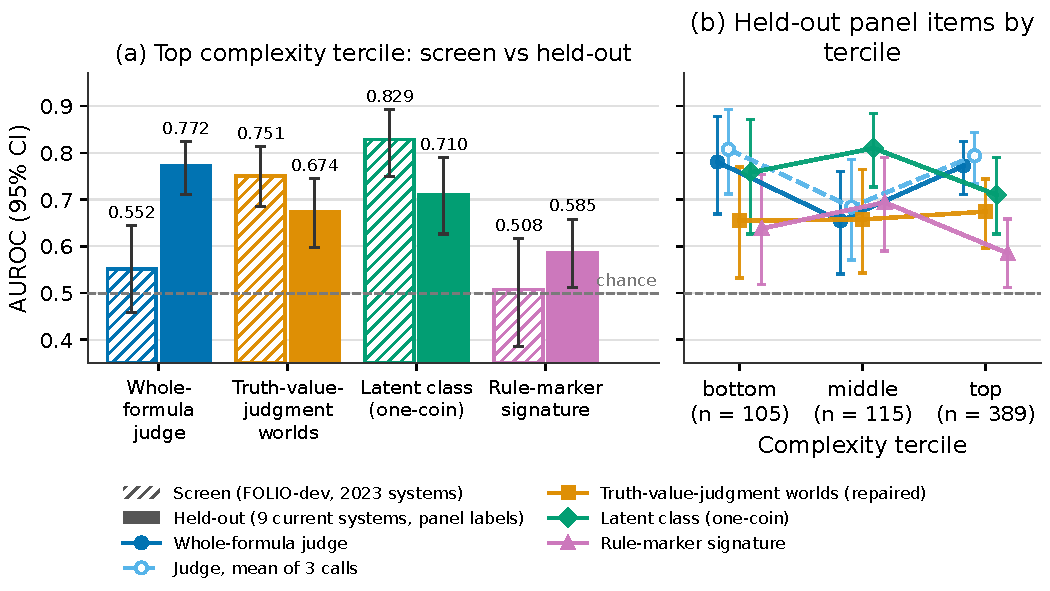
\includegraphics[width=\linewidth,height=0.85\textheight,keepaspectratio]{figures/figR5_v0.pdf}
\caption{Panel (a): AUROC in the top complexity tercile on the iteration-1 FOLIO-dev screen (Logic-LM candidates; worlds, latent class and judge against Arm B labels, n = 833 overall; rule-marker signature against Arm A labels) and on the held-out panel items (389 top-tercile items, post-stratified weights; truth-value-judgment worlds in their repaired, frozen form). Panel (b): held-out panel AUROC by tercile (bottom n = 105, middle n = 115, top n = 389). The judge fell to 0.552 on the screen's top tercile but scores 0.772 on held-out top-tercile items, where the worlds are 0.098 below it.}
\label{fig:figR5}
\end{figure}

Table 140 gives the pre-registered tests and the decision table. The primary test, the top-tercile gap, has an upper bound below zero, so the pre-registered label is \emph{reversed}. The growth test is not significant, and the gap by number of conditions is not monotone. The interaction slopes of a weighted logistic model lean the predicted way (worlds +0.104, judge $-$0.166), but the joint contrast includes zero, and the worlds sit below the judge at every level.

{\small
\setlength{\tabcolsep}{3pt}
\begin{longtable}{>{\raggedright\arraybackslash}p{0.394\linewidth}>{\raggedright\arraybackslash}p{0.253\linewidth}>{\raggedright\arraybackslash}p{0.304\linewidth}}
\caption*{\textbf{Table 140.} Pre-registered tests for the worlds (repaired, frozen) against the judge, and the decision table. \textit{[Source: the earlier run's round-2 truth-value-judgment deep-test artifact (earlier run, iteration 2)]}}\\
\toprule
\textbf{Test} & \textbf{Estimate [95\% CI]} & \textbf{Outcome} \\
\midrule
\endfirsthead
\multicolumn{3}{l}{\textit{(continued)}}\\
\toprule
\textbf{Test} & \textbf{Estimate [95\% CI]} & \textbf{Outcome} \\
\midrule
\endhead
\bottomrule
\endlastfoot
{}top-tercile gap, worlds $-$ judge (primary) & $-$0.098 [$-$0.184, $-$0.014] & reversed \\
{}growth, gap(top) $-$ gap(bottom) & +0.028 [$-$0.126, +0.186] & n.s. \\
{}gap by conditions 0-1 / 2-3 / 4+ & $-$0.003 / $-$0.157 / $-$0.060 & not monotone \\
{}interaction slope, worlds & +0.104 [$-$0.150, +0.348] & n.s. \\
{}interaction slope, judge & $-$0.166 [$-$0.442, +0.177] & n.s. \\
{}joint contrast of slopes & +0.375 [$-$0.081, +0.803] & n.s. \\
{}top-tercile gap, worlds $-$ judge (mean of 3 calls) & $-$0.120 [$-$0.208, $-$0.035] & judge-matched: no \\
{}all-panel gap, worlds $-$ judge & $-$0.084 [$-$0.144, $-$0.026] &  \\
{}all-panel gap, repaired $-$ iteration-1 worlds & $-$0.020 [$-$0.066, +0.023] & repair adds no discrimination \\
{}all-panel gap, latent class $-$ judge & +0.007 [$-$0.051, +0.061] &  \\
{}all-panel gap, rule-marker $-$ judge & $-$0.109 [$-$0.185, $-$0.039] &  \\
{}all-panel gap, latent class $-$ rule-marker & +0.116 [0.044, 0.193] &  \\
{}worlds added to [judge, parse, latent class, rule-marker] & $-$0.002 [$-$0.008, +0.003] & stack increment: no \\
{}repair: screen and held-out paired false alarms $\leq$ 0.10 & screen 0.212, held-out 0.077 & repair ok: no (renaming only) \\
\end{longtable}
}

The stacking results in Table 141 make the same point from another side. Adding the worlds to [judge + parse rate] gives +0.011 with a CI spanning zero. Adding latent class and the rule-marker signature to the same base gives +0.061, significant. We call that model, the judge and parse rate plus the two zero-LLM metrics, the \emph{judge-plus-zero-LLM stack}; adding the worlds on top of it gives nothing. A shuffled placebo feature gives $-$0.003.

\begin{table}[H]
\centering
\small
\setlength{\tabcolsep}{3pt}
\caption*{\textbf{Table 141.} Cross-fitted stacks on the panel items (sentence-grouped 5-fold, weighted logistic). \textit{[Source: the earlier run's round-2 truth-value-judgment deep-test artifact (earlier run, iteration 2)]}}
\begin{tabular}{>{\raggedright\arraybackslash}p{0.405\linewidth}>{\raggedright\arraybackslash}p{0.154\linewidth}>{\raggedright\arraybackslash}p{0.392\linewidth}}
\toprule
\textbf{Stack} & \textbf{weighted AUROC} & \textbf{contrast [95\% CI]} \\
\midrule
{}judge + parse & 0.741 &  \\
{}judge + parse + worlds & 0.753 & vs judge + parse: +0.011 [$-$0.017, +0.039] \\
{}judge + parse + latent class + rule-marker (judge-plus-zero-LLM stack) & 0.802 & vs judge + parse: +0.061 [0.013, 0.106] \\
{}judge + parse + worlds + latent class + rule-marker & 0.800 & vs judge-plus-zero-LLM stack: $-$0.002 [$-$0.008, +0.003] \\
{}latent class alone (cross-fitted) & 0.710 & judge-plus-zero-LLM stack vs latent class: +0.092 [0.058, 0.126] \\
{}judge-plus-zero-LLM stack vs raw latent-class score &  & +0.046 [0.007, 0.082] \\
{}judge + parse + shuffled placebo & 0.738 & vs judge + parse: $-$0.003 [$-$0.028, +0.023] \\
\bottomrule
\end{tabular}
\end{table}

The judged false-alarm replication on held-out used 99 audited golds and 183 scored rewrites (\$0.12). Reorder (46), contrapositive (51), De Morgan (31) and prenex (2) rewrites all had a paired false-alarm rate of 0.000; renaming (53) had 0.264, for 0.077 overall. The pre-registered repair criterion therefore fails, through renaming only. The plan had anticipated this outcome as a verbalizer limitation: a world written with a synonym-renamed predicate reads differently against the sentence.

\subsubsection{Real error types, and the error-type naming test}

Table 142 gives detection by the panel's primary error type: the probability that an erroneous candidate scores below a faithful candidate of the same sentence (a faithful candidate from another sentence is used when none exists; ``fallback'' counts those). The repaired worlds are below the judge on every well-populated type. On the 17 scope and cardinality errors, the signature's predicted blind spots, the worlds (0.743) beat the rule-marker signature (0.614) but not the judge (0.812) or latent class (0.806). All CIs there are wide.

{\footnotesize
\setlength{\tabcolsep}{3pt}
\begin{longtable}{>{\raggedright\arraybackslash}p{0.118\linewidth}>{\raggedright\arraybackslash}p{0.139\linewidth}>{\raggedright\arraybackslash}p{0.112\linewidth}>{\raggedright\arraybackslash}p{0.125\linewidth}>{\raggedright\arraybackslash}p{0.071\linewidth}>{\raggedright\arraybackslash}p{0.085\linewidth}>{\raggedright\arraybackslash}p{0.085\linewidth}>{\raggedright\arraybackslash}p{0.152\linewidth}}
\caption*{\textbf{Table 142.} Detection by real error type on panel items (Wilson intervals omitted; n unfaithful, of which ``fallback'' used a faithful item from another sentence). \textit{[Source: the earlier run's round-2 truth-value-judgment deep-test artifact (earlier run, iteration 2)]}}\\
\toprule
\textbf{Error type} & \textbf{n (fallback)} & \textbf{worlds, repaired} & \textbf{worlds, iteration 1} & \textbf{judge} & \textbf{judge, 3 calls} & \textbf{latent class} & \textbf{rule-marker} \\
\midrule
\endfirsthead
\multicolumn{8}{l}{\textit{(continued)}}\\
\toprule
\textbf{Error type} & \textbf{n (fallback)} & \textbf{worlds, repaired} & \textbf{worlds, iteration 1} & \textbf{judge} & \textbf{judge, 3 calls} & \textbf{latent class} & \textbf{rule-marker} \\
\midrule
\endhead
\bottomrule
\endlastfoot
{}added condition & 74 (47) & 0.600 & 0.648 & 0.686 & 0.702 & 0.717 & 0.628 \\
{}$\forall$/$\exists$ choice & 60 (42) & 0.551 & 0.613 & 0.795 & 0.812 & 0.797 & 0.496 \\
{}dropped condition & 47 (26) & 0.629 & 0.677 & 0.658 & 0.713 & 0.624 & 0.733 \\
{}implication direction / ``only'' & 29 (18) & 0.577 & 0.705 & 0.695 & 0.718 & 0.760 & 0.849 \\
{}quantifier scope & 16 (10) & 0.758 & 0.649 & 0.831 & 0.856 & 0.825 & 0.621 \\
{}conflation & 16 (11) & 0.734 & 0.625 & 0.776 & 0.715 & 0.638 & 0.665 \\
{}conjunction / disjunction & 14 (10) & 0.651 & 0.581 & 0.804 & 0.855 & 0.782 & 0.714 \\
{}negation / polarity & 10 (8) & 0.663 & 0.602 & 0.868 & 0.879 & 0.701 & 0.696 \\
{}wrong constant & 9 (6) & 0.196 & 0.343 & 0.395 & 0.413 & 0.582 & 0.532 \\
{}argument swap & 4 (3) & 0.582 & 0.640 & 0.751 & 0.785 & 0.649 & 0.345 \\
{}cardinality / numeric & 1 (0) & 0.500 & 0.500 & 0.500 & 0.500 & 0.500 & 0.500 \\
{}scope $\cup$ cardinality & 17 (10) & 0.743 & 0.640 & 0.812 & 0.835 & 0.806 & 0.614 \\
\end{longtable}
}

The worlds' error-type naming (the mutant operator whose worlds the candidate loses most) was scored on 271 typed unfaithful items. Its accuracy was 0.077, below the 0.273 of always predicting the most common type, with macro-F1 0.079.

\subsubsection{Top-tercile population, contamination, system level and cost}

On all 2,826 top-tercile candidates with soft labels, the repaired worlds (0.609 [0.590, 0.626]) tie the judge (0.608 [0.593, 0.624]), and latent class (0.646) and majority agreement (0.658) lead; the rule-marker signature scores 0.573 and parse rate 0.513. Multiple imputation of the labels gives the same values. Under hard solver labels on 2,546 rows, which favour gold vocabulary, the worlds score 0.679, the judge 0.718, latent class 0.792 and majority agreement 0.801.

On the contamination rows, neither the worlds (AUROC shift +0.002 [$-$0.040, +0.040]) nor the judge (+0.009 [$-$0.038, +0.055]) nor latent class ($-$0.001) changed between originals and paraphrases. Mean scores dropped on paraphrases by 0.058 for the worlds, 0.100 for the judge and 0.144 for the rule-marker signature, whose lexical aligner is name-sensitive; latent class did not move.

System-level $\tau$ was computed only for the zero-LLM metrics in this artifact: against panel accuracy, latent class 0.500, majority agreement 0.556, rule-marker 0.722 and parse rate 0.535; against soft accuracy, 0.833, 0.778, 0.833 and 0.761. With nine systems \textbar{}$\tau$\textbar{} $\geq$ 0.61 is needed for p $<$ 0.05, so these are descriptive only.

Per item the repaired worlds cost \$0.00066 (three votes, median 2.9 s) and the judge \$0.000028 (0.6 s). The worlds are 24 times more expensive and less accurate. Total OpenRouter spend was \$4.10.

\subsubsection{Dead ends in this artifact}

\begin{itemize}
\item {}A local judge for the worlds, tried while the key was down. Qwen2.5-1.5B and 3B via llama.cpp agreed with world truth at 0.54 and 0.44 on 8 panel items, chance level; no local result is reported.
\item {}The flash-lite judge, the cheaper variant the plan asked for: 0.565 on the panel, 0.184 below the judge.
\item {}The repair as a source of discrimination. It removed the false alarms and lowered held-out AUROC by 0.020.
\item {}The complexity crossover itself, the reason this artifact existed. The artifact's reading, which we share, is that the iteration-1 crossover was a property of the Logic-LM FOLIO-dev screen and its equivalence labels: there the judge fell to 0.552 in the top tercile, and on held-out sentences from nine current systems it scores 0.772 there.
\end{itemize}
\subsection{Round 2, part 4: The monotonicity signature as an error-type classifier and wrong-gold flagger}

\subsubsection{Phase 1: three repairs, tuned on the screen only}

The screen's 300 sentences were split by SHA-1 into 150 development and 150 test sentences. A regression test first reproduced the iteration-1 rule-marker signature and alignment-only control exactly on 50 screen items each.

\emph{Aligner.} The iteration-1 greedy lemma matching was replaced by a global assignment between sentence concepts and predicates, solved with the Hungarian method [41]. The similarity is the maximum of lemma and camelCase overlap, WordNet [40] path similarity, and MiniLM cosine, plus an arity term; it uses no polarity information, to keep the aligner from seeing what it is later compared against. A pre-registered rule chose among grid configurations: keep configurations whose mutant detection for six operators drops by no more than 0.03 and whose logical-rewrite false alarms rise by no more than 0.01, then minimise renaming false alarms. The chosen threshold was 0.55, with path similarity, MiniLM and arity weight 0.1. It cut screen-test renaming false alarms from 0.419 to 0.129, but missed the pre-registered 0.05 target (Table 143). On an unseen set of 134 renamings written by gpt-4.1-mini to avoid dictionary synonyms (for example \texttt{IsAGreatPlace} $\rightarrow$ \texttt{ExcellentLocation}), false alarms were 0.515 against 0.575 for the old aligner. The pre-registered fallback with a larger embedding model broke detection of added conditions and was rejected.

{\small
\setlength{\tabcolsep}{3pt}
\begin{longtable}{>{\raggedright\arraybackslash}p{0.418\linewidth}>{\raggedright\arraybackslash}p{0.242\linewidth}>{\raggedright\arraybackslash}p{0.292\linewidth}}
\caption*{\textbf{Table 143.} Aligner repair on the 150 screen-test sentences (417 real candidates). Detection is the pairwise mutant detection rate. \textit{[Source: the earlier run's round-2 signature classifier and wrong-gold flagger artifact (earlier run, iteration 2)]}}\\
\toprule
\textbf{Measure} & \textbf{repaired aligner} & \textbf{iteration-1 aligner} \\
\midrule
\endfirsthead
\multicolumn{3}{l}{\textit{(continued)}}\\
\toprule
\textbf{Measure} & \textbf{repaired aligner} & \textbf{iteration-1 aligner} \\
\midrule
\endhead
\bottomrule
\endlastfoot
{}synonym-rename false alarms (n = 62) & 0.129 & 0.419 \\
{}unseen gpt-4.1-mini renames (n = 134) & 0.515 & 0.575 \\
{}contrapositive false alarms (n = 54) & 0.019 & 0.000 \\
{}reorder / De Morgan / prenex false alarms & 0.000 & 0.000 \\
{}AUROC on real candidates & 0.738 & 0.732 \\
{}detection: added / dropped condition & 0.820 / 0.765 & 0.827 / 0.775 \\
{}detection: negation / $\forall$$\exists$ / implication reversal & 0.810 / 0.669 / 0.737 & 0.787 / 0.682 / 0.737 \\
{}detection: argument swap / merge & 0.618 / 0.842 & 0.588 / 0.804 \\
{}detection: and/or / cardinality & 0.517 / 0.500 & 0.508 / 0.500 \\
\end{longtable}
}

\emph{Text side.} Five text sides were compared on a MED/HELP development split, in probe style (two specialized copies, up and down questions per edited concept). The rule was to maximise the mean of balanced MED/HELP accuracy and a silver accuracy on screen golds, subject to downward accuracy no worse than the rules minus 0.02. The chosen side keeps the rule-based label, except where the rules say upward and the gemini probe says downward consistently on both specialized copies. A second side used the probe whenever its two copies agreed and fell back on the rules otherwise; a third used the probe alone. A side that let gpt-5-mini decide rule-probe disagreements tied it and lost the tie-break on cost; gemini-2.5-pro was ineligible because its projected full-run cost (\$1.72) exceeded the \$1.50 cap. On the MED/HELP test split (Table 144) the chosen side reached 0.949 downward accuracy against 0.847 for the rules, which clears the 0.85 the hypothesis had assumed. On held-out golds judged faithful by the panel, agreement between the text label and the gold's solver label was 0.748 against 0.635 for the rules, and 0.648 against 0.435 on downward concepts.

\begin{table}[H]
\centering
\footnotesize
\setlength{\tabcolsep}{3pt}
\caption*{\textbf{Table 144.} Text-side accuracy on the MED/HELP test split (439 usable items after dropping 131 multi-span and 30 no-concept items). Rules = rule marker; probe = gemini-2.5-flash substitution probe with a 1,024-token thinking budget. \textit{[Source: the earlier run's round-2 signature classifier and wrong-gold flagger artifact (earlier run, iteration 2)]}}
\begin{tabular}{>{\raggedright\arraybackslash}p{0.237\linewidth}>{\raggedright\arraybackslash}p{0.116\linewidth}>{\raggedright\arraybackslash}p{0.103\linewidth}>{\raggedright\arraybackslash}p{0.151\linewidth}>{\raggedright\arraybackslash}p{0.089\linewidth}>{\raggedright\arraybackslash}p{0.074\linewidth}>{\raggedright\arraybackslash}p{0.131\linewidth}}
\toprule
\textbf{Text side} & \textbf{overall} & \textbf{upward (224)} & \textbf{downward (215)} & \textbf{MED down (128)} & \textbf{HELP down (87)} & \textbf{balanced} \\
\midrule
{}rules only & 0.879 & 0.911 & 0.847 & 0.844 & 0.851 & 0.879 \\
{}probe only & 0.763 & 0.879 & 0.642 & 0.594 & 0.713 & 0.761 \\
{}probe when its two copies agree, else rules & 0.888 & 0.973 & 0.800 & 0.797 & 0.805 & 0.887 \\
{}rules, overridden where the probe consistently says downward and the rules say upward (chosen) & 0.925 & 0.902 & 0.949 [0.91, 0.97] & 0.953 & 0.943 & 0.925 \\
\bottomrule
\end{tabular}
\end{table}

Held-out silver agreement by corpus was FOLIO 0.912 (rules 0.824), MALLS 0.739 (0.597) and ProverQA 0.651 (0.564).

\emph{Error-type classifier.} The signature mismatch vector is mapped to the error taxonomy by a weighted rule list (the \emph{rule classifier}) whose weights were calibrated on screen-development mutants (macro-F1 0.465 there). A logistic regression over the same mismatch features (the \emph{logistic classifier}) was carried alongside because it beat the rules on screen-test macro-F1 by at least 0.05 (0.453 against 0.389). On screen-test mutants the rule classifier had top-1 accuracy 0.40 and top-2 0.59; per type, top-1 ranged from 0.03 for and/or swaps to 0.67 for dropped conditions. On the 37 scope-swap mutants of the blind-spot supplement, detection was exactly 0.5, as built.

The configuration, classifier weights and a SHA-256 of the module source were written to a frozen file, and a firewall checked that the held-out labels were closed before and open only after it. The label counts (307/302) were printed once while checking field formats.

\subsubsection{Phase 2: pre-registered verdicts}

The LLM baseline for error typing is a \emph{typed judge}: gemini-2.5-flash is shown the sentence and the candidate and asked to pick one error type from the same taxonomy. All five pre-registered verdicts failed or were not confirmed (Table 145).

\begin{table}[H]
\centering
\small
\setlength{\tabcolsep}{3pt}
\caption*{\textbf{Table 145.} Pre-registered verdicts of the signature artifact on held-out data. \textit{[Source: the earlier run's round-2 signature classifier and wrong-gold flagger artifact (earlier run, iteration 2)]}}
\begin{tabular}{>{\raggedright\arraybackslash}p{0.273\linewidth}>{\raggedright\arraybackslash}p{0.181\linewidth}>{\raggedright\arraybackslash}p{0.498\linewidth}}
\toprule
\textbf{Verdict} & \textbf{Outcome} & \textbf{Evidence} \\
\midrule
{}error-type naming beats an LLM typer & fail & rule classifier weighted top-1 0.111 vs typed gemini judge 0.302: $\Delta$ $-$0.19 [$-$0.26, $-$0.12], McNemar p = 1.5e-7 \\
{}wrong-gold flagging works & fail (one clause) & pooled AUROC 0.673 $>$ 0.5; ProverQA precision@25 0.40; enrichment@50 0.58; but the concept-coverage control (0.686) scores at least as high \\
{}polarity carries signal beyond alignment & fail & +0.011 [$-$0.010, 0.031] over [judge, parse, alignment-only] \\
{}renaming fixed & fail & screen rename false alarms 0.129; unseen renames 0.515; full signature match on correct-but-inequivalent candidates 0.256 (target 0.80) \\
{}blind spots confirmed on real errors & not confirmed & predicted-visible detection 0.73 [0.67, 0.79] $<$ 0.80; predicted-blind 0.59 [0.43, 0.77], n = 23 \\
\bottomrule
\end{tabular}
\end{table}

\subsubsection{Ranking: the repaired signature is still below its controls}

As a ranking metric the repaired signature scores 0.654 on the panel, below the alignment-only (0.673) and concept-coverage (0.674) controls and below the judge (0.745) and the typed judge (0.777). The polarity-only component scores 0.580 (Table 146). The repaired signature is 0.015 above the unrepaired rule-marker signature. When labels are shuffled \emph{within} sentences, the signature keeps an AUROC of 0.648, so most of its item-level signal separates sentences rather than candidates.

{\footnotesize
\setlength{\tabcolsep}{3pt}
\begin{longtable}{>{\raggedright\arraybackslash}p{0.209\linewidth}>{\raggedright\arraybackslash}p{0.103\linewidth}>{\raggedright\arraybackslash}p{0.099\linewidth}>{\raggedright\arraybackslash}p{0.099\linewidth}>{\raggedright\arraybackslash}p{0.083\linewidth}>{\raggedright\arraybackslash}p{0.083\linewidth}>{\raggedright\arraybackslash}p{0.083\linewidth}>{\raggedright\arraybackslash}p{0.129\linewidth}}
\caption*{\textbf{Table 146.} Standalone weighted AUROC on the 609 panel items, overall [95\% CI], by tercile and by corpus. \textit{[Source: the earlier run's round-2 signature classifier and wrong-gold flagger artifact (earlier run, iteration 2)]}}\\
\toprule
\textbf{Metric} & \textbf{all} & \textbf{bottom (105)} & \textbf{middle (115)} & \textbf{top (389)} & \textbf{FOLIO (238)} & \textbf{MALLS (224)} & \textbf{ProverQA (147)} \\
\midrule
\endfirsthead
\multicolumn{8}{l}{\textit{(continued)}}\\
\toprule
\textbf{Metric} & \textbf{all} & \textbf{bottom (105)} & \textbf{middle (115)} & \textbf{top (389)} & \textbf{FOLIO (238)} & \textbf{MALLS (224)} & \textbf{ProverQA (147)} \\
\midrule
\endhead
\bottomrule
\endlastfoot
{}repaired signature & 0.654 [0.598, 0.709] & 0.651 & 0.708 & 0.608 & 0.615 & 0.720 & 0.593 \\
{}polarity component only & 0.580 [0.524, 0.634] & 0.585 & 0.579 & 0.563 & 0.583 & 0.638 & 0.455 \\
{}alignment-only (repaired aligner) & 0.673 [0.623, 0.719] & 0.674 & 0.716 & 0.630 & 0.605 & 0.727 & 0.696 \\
{}concept coverage (repaired aligner) & 0.674 [0.624, 0.722] & 0.655 & 0.730 & 0.646 & 0.599 & 0.714 & 0.699 \\
{}rule-marker signature, iteration 1 & 0.639 [0.585, 0.693] & 0.636 & 0.694 & 0.584 & 0.585 & 0.719 & 0.579 \\
{}alignment-only, iteration 1 & 0.656 [0.604, 0.704] & 0.675 & 0.670 & 0.612 & 0.577 & 0.696 & 0.721 \\
{}whole-formula judge & 0.745 [0.699, 0.791] & 0.785 & 0.661 & 0.758 & 0.731 & 0.676 & 0.850 \\
{}typed judge & 0.777 [0.726, 0.823] & 0.796 & 0.773 & 0.728 & 0.763 & 0.618 & 0.912 \\
{}parse rate & 0.500 & 0.500 & 0.500 & 0.500 & 0.500 & 0.500 & 0.500 \\
\end{longtable}
}

The polarity increment is not significant with the repaired text side either (Table 147): adding the polarity component to [judge, parse, alignment-only] gives +0.011, and a within-sentence shuffle placebo gives about the same (+0.010). Adding the full repaired signature to the judge alone gives a significant +0.057.

\begin{table}[H]
\centering
\small
\setlength{\tabcolsep}{3pt}
\caption*{\textbf{Table 147.} Polarity increment on panel items (cross-fitted, out-of-fold AUROC). \textit{[Source: the earlier run's round-2 signature classifier and wrong-gold flagger artifact (earlier run, iteration 2)]}}
\begin{tabular}{>{\raggedright\arraybackslash}p{0.532\linewidth}>{\raggedright\arraybackslash}p{0.120\linewidth}>{\raggedright\arraybackslash}p{0.299\linewidth}}
\toprule
\textbf{Model} & \textbf{OOF AUROC} & \textbf{increment [95\% CI]} \\
\midrule
{}judge + parse + alignment-only & 0.777 &  \\
{}+ repaired signature & 0.786 & +0.009 [$-$0.012, 0.029] \\
{}+ polarity component & 0.788 & +0.011 [$-$0.010, 0.031] \\
{}judge + parse + iteration-1 alignment-only & 0.765 &  \\
{}+ iteration-1 rule-marker signature & 0.771 & +0.006 [$-$0.011, 0.023] \\
{}judge only & 0.713 &  \\
{}judge + repaired signature & 0.770 & +0.057 [0.008, 0.104] \\
{}within-sentence shuffle placebo, polarity component &  & +0.010 [$-$0.008, 0.029] \\
\bottomrule
\end{tabular}
\end{table}

\subsubsection{Error-type naming}

On the 302 panel-unfaithful items, the typed judge (gemini-2.5-flash shown sentence and candidate and asked for one type) named the panel's primary type 0.302 of the time. The rule classifier managed 0.111, below always answering ``added condition'' (0.249) and the prior-matched random expectation (0.150). The logistic classifier (0.145) and a thinking typed judge (0.281) did not change the ordering. The union of rule classifier and typed judge reached 0.370. The ceiling is low for everyone: the panel members agreed with each other on the primary type only 0.37 of the time pairwise, and 0.55 in a leave-one-member-out comparison. With truth labels permuted, the rule classifier still scored 0.090, barely below its real value.

\begin{landscape}
{\footnotesize
\setlength{\tabcolsep}{3pt}
\begin{longtable}{>{\raggedright\arraybackslash}p{0.124\linewidth}>{\raggedright\arraybackslash}p{0.047\linewidth}>{\raggedright\arraybackslash}p{0.047\linewidth}>{\raggedright\arraybackslash}p{0.064\linewidth}>{\raggedright\arraybackslash}p{0.073\linewidth}>{\raggedright\arraybackslash}p{0.047\linewidth}>{\raggedright\arraybackslash}p{0.038\linewidth}>{\raggedright\arraybackslash}p{0.064\linewidth}>{\raggedright\arraybackslash}p{0.099\linewidth}>{\raggedright\arraybackslash}p{0.047\linewidth}>{\raggedright\arraybackslash}p{0.090\linewidth}>{\raggedright\arraybackslash}p{0.056\linewidth}>{\raggedright\arraybackslash}p{0.073\linewidth}}
\caption*{\textbf{Table 148.} Error-type naming on 302 panel-unfaithful items (weighted). Recall per type is shown for types with n $\geq$ 10. \textit{[Source: the earlier run's round-2 signature classifier and wrong-gold flagger artifact (earlier run, iteration 2)]}}\\
\toprule
\textbf{Method} & \textbf{top-1} & \textbf{top-2} & \textbf{lenient} & \textbf{macro-F1} & \textbf{added (74)} & \textbf{$\forall$/$\exists$ (60)} & \textbf{dropped (47)} & \textbf{implication (29)} & \textbf{scope (16)} & \textbf{conflation (16)} & \textbf{and/or (14)} & \textbf{negation (10)} \\
\midrule
\endfirsthead
\multicolumn{13}{l}{\textit{(continued)}}\\
\toprule
\textbf{Method} & \textbf{top-1} & \textbf{top-2} & \textbf{lenient} & \textbf{macro-F1} & \textbf{added (74)} & \textbf{$\forall$/$\exists$ (60)} & \textbf{dropped (47)} & \textbf{implication (29)} & \textbf{scope (16)} & \textbf{conflation (16)} & \textbf{and/or (14)} & \textbf{negation (10)} \\
\midrule
\endhead
\bottomrule
\endlastfoot
{}rule classifier (frozen) & 0.111 & 0.194 & 0.297 & 0.086 & 0.08 & 0.10 & 0.43 & 0.03 & 0.00 & 0.00 & 0.14 & 0.10 \\
{}logistic classifier & 0.145 & 0.245 & 0.360 & 0.091 & 0.42 & 0.15 & 0.06 & 0.10 & 0.00 & 0.00 & 0.07 & 0.00 \\
{}typed judge (gemini-2.5-flash) & 0.302 & 0.344 & 0.532 & 0.269 & 0.03 & 0.65 & 0.26 & 0.52 & 0.06 & 0.00 & 0.86 & 0.50 \\
{}typed judge, thinking & 0.281 & 0.314 & 0.484 & 0.343 & 0.11 & 0.57 & 0.17 & 0.48 & 0.19 & 0.44 & 0.50 & 0.20 \\
{}iteration-1 rules & 0.079 & 0.079 & 0.261 & 0.066 & 0.05 & 0.00 & 0.28 & 0.00 & 0.00 & 0.56 & 0.07 & 0.00 \\
{}always ``added condition'' & 0.249 & 0.467 & 0.647 & 0.044 & 1.00 & 0.00 & 0.00 & 0.00 & 0.00 & 0.00 & 0.00 & 0.00 \\
\end{longtable}
}
\end{landscape}

The 29 unfaithful items with no signature change at all, the predicted blind-spot bucket, were mostly $\forall$/$\exists$ (11) and added-condition (6) errors; only 17\% belonged to the predicted blind types.

\subsubsection{Detection within a sentence, and the blind spots}

Table 149 compares each erroneous candidate with faithful candidates of the same sentence from other systems. This is where the signature does its best work. It detects dropped conditions at 0.853 and implication-direction errors at 0.866, above the judge (0.618 and 0.770) and the typed judge (0.486 and 0.530), which were scored on the subset of items they covered. It is weak on $\forall$/$\exists$ (0.616), where the typed judge reaches 0.918. The pre-registered blind-spot test is not confirmed: detection on the predicted-visible types is 0.73, short of the 0.80 bar, and the 23 predicted-blind errors give 0.59 with a CI that contains 0.5 but overlaps the visible one. A random score gives 0.499.

{\footnotesize
\setlength{\tabcolsep}{3pt}
\begin{longtable}{>{\raggedright\arraybackslash}p{0.119\linewidth}>{\raggedright\arraybackslash}p{0.035\linewidth}>{\raggedright\arraybackslash}p{0.127\linewidth}>{\raggedright\arraybackslash}p{0.195\linewidth}>{\raggedright\arraybackslash}p{0.154\linewidth}>{\raggedright\arraybackslash}p{0.113\linewidth}>{\raggedright\arraybackslash}p{0.072\linewidth}>{\raggedright\arraybackslash}p{0.072\linewidth}}
\caption*{\textbf{Table 149.} Within-sentence detection by real error type (P(error scores below a faithful partner); n errors with a partner; the judges were scored only on the items they covered, n in parentheses). Types with n $<$ 10 are descriptive. \textit{[Source: the earlier run's round-2 signature classifier and wrong-gold flagger artifact (earlier run, iteration 2)]}}\\
\toprule
\textbf{Error type} & \textbf{n} & \textbf{repaired signature} & \textbf{alignment-only} & \textbf{iteration-1 rule-marker} & \textbf{polarity only} & \textbf{judge (n)} & \textbf{typed judge (n)} \\
\midrule
\endfirsthead
\multicolumn{8}{l}{\textit{(continued)}}\\
\toprule
\textbf{Error type} & \textbf{n} & \textbf{repaired signature} & \textbf{alignment-only} & \textbf{iteration-1 rule-marker} & \textbf{polarity only} & \textbf{judge (n)} & \textbf{typed judge (n)} \\
\midrule
\endhead
\bottomrule
\endlastfoot
{}added condition & 65 & 0.760 & 0.660 & 0.656 & 0.681 & 0.747 (24) & 0.546 (24) \\
{}dropped condition & 36 & 0.853 & 0.852 & 0.777 & 0.469 & 0.618 (21) & 0.486 (21) \\
{}$\forall$/$\exists$ choice & 56 & 0.616 & 0.579 & 0.504 & 0.578 & 0.662 (17) & 0.918 (17) \\
{}implication direction & 24 & 0.866 & 0.598 & 0.870 & 0.832 & 0.770 (11) & 0.530 (11) \\
{}quantifier scope & 12 & 0.559 & 0.509 & 0.482 & 0.543 & 0.985 (6) & 0.442 (6) \\
{}conjunction / disjunction & 10 & 0.741 & 0.510 & 0.697 & 0.745 & 0.595 (4) & 1.000 (4) \\
{}negation / polarity & 5 & 0.588 & 0.485 & 0.588 & 0.698 & 1.000 (2) & 1.000 (2) \\
{}argument swap & 2 & 0.121 & 0.241 & 0.121 & 0.379 & 0.500 (1) & 1.000 (1) \\
{}cardinality & 1 & 0.375 & 0.375 & 0.375 & 0.500 & n/a & n/a \\
{}predicted visible (pooled) & 188 & 0.727 [0.669, 0.786] & 0.650 & 0.642 & 0.622 & 0.695 (76) & 0.630 (76) \\
{}predicted blind (pooled) & 23 & 0.591 [0.433, 0.766] & 0.488 & 0.538 & 0.604 & 0.886 (10) & 0.583 (10) \\
\end{longtable}
}

\begin{correction}\textbf{Correction (iteration 2).} The judge and typed-judge columns above were scored only on the items those judges happened to cover (21 and 11 on the two headline classes). Re-scored with the frozen cheap judge on 34 of the 36 dropped-condition and 21 of the 24 implication-direction errors, the judge detects them at 0.577 and 0.576, and the round-trip and agreement baselines join the comparison (Table 37). These two classes were singled out after the fact from nine; the pre-registered blind-spot test on the pooled classes was not confirmed (Table 145).\end{correction}

Figure~\ref{fig:figR6} draws the first six rows of Table 149.

\begin{figure}[!htbp]
\centering
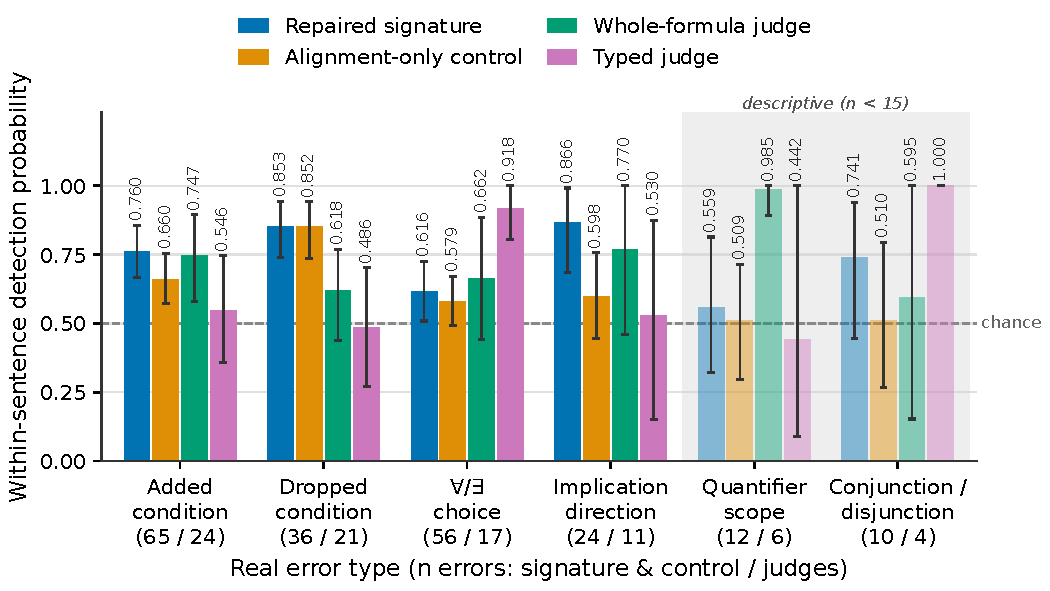
\includegraphics[width=\linewidth,height=0.85\textheight,keepaspectratio]{figures/figR6_v0.pdf}
\caption{Within-sentence detection by real (panel-typed) error type on held-out data: probability that an erroneous candidate scores below a faithful candidate of the same sentence (0.5 = chance). The signature and alignment-only control were scored on every item with a partner; the judges only on the items they covered (n in the category labels). The repaired signature leads on dropped conditions and implication-direction errors and trails the typed judge on the $\forall$/$\exists$ choice. Post hoc: the two leading classes were singled out from nine after the data were seen, the judges were scored only on the items they happened to cover, and with the cheap judge re-scored on all available pairs it detects dropped-condition and implication-direction errors at 0.577 and 0.576 (Table 37).}
\label{fig:figR6}
\end{figure}

\subsubsection{Correct-but-gold-inequivalent candidates (criterion 5)}

Success criterion 5 of the hypothesis asked that at least 80\% of adjudicated correct-but-gold-inequivalent candidates get a full signature match. On the 250 panel-faithful, solver-non-equivalent items, the repaired signature gave a full match to 25.6\% (iteration-1 signature 21.2\%), with mean score 0.769 (0.726). The whole-formula judge scored only 2.4\% of these items below 0.5, and the typed judge falsely named an error for 42.8\% of them.

\subsubsection{Wrong-gold flagging}

Run text-against-gold on the 700 held-out golds, the signature flags panel-judged wrong gold at pooled AUROC 0.673 (Table 150). Its best corpus is MALLS, where 23 of its top 25 flags are wrong gold (precision 0.92 against a base rate of 0.456). On ProverQA its precision@25 is 0.40 against a base rate of 0.175, the one clause of the hypothesis's gold-error criterion (precision@k at least twice the base rate) that holds; at @50 it falls to 0.24. The alignment-only and concept-coverage controls do as well or better, and the LLM judges run on the gold do much better (0.840 and 0.859). The signature is still complementary to the judge: adding it to the judge raises gold-flag AUROC from 0.808 to 0.861 (+0.054 [0.029, 0.079]).

\begin{table}[H]
\centering
\footnotesize
\setlength{\tabcolsep}{3pt}
\caption*{\textbf{Table 150.} Wrong-gold flagging: score of the gold formula against the panel's gold verdict (flag = low score). AUROC [95\% CI], precision@25 and @50. \textit{[Source: the earlier run's round-2 signature classifier and wrong-gold flagger artifact (earlier run, iteration 2)]}}
\begin{tabular}{>{\raggedright\arraybackslash}p{0.134\linewidth}>{\raggedright\arraybackslash}p{0.113\linewidth}>{\raggedright\arraybackslash}p{0.101\linewidth}>{\raggedright\arraybackslash}p{0.174\linewidth}>{\raggedright\arraybackslash}p{0.101\linewidth}>{\raggedright\arraybackslash}p{0.137\linewidth}>{\raggedright\arraybackslash}p{0.064\linewidth}>{\raggedright\arraybackslash}p{0.064\linewidth}}
\toprule
\textbf{Corpus (n, base rate)} & \textbf{repaired signature} & \textbf{polarity only} & \textbf{alignment-only} & \textbf{concept coverage} & \textbf{iteration-1 rule-marker} & \textbf{judge on gold} & \textbf{typed judge on gold} \\
\midrule
{}pooled (700, 0.434) & 0.673 [0.634, 0.712]; 0.72 / 0.76 & 0.547; 0.72 / 0.70 & 0.690; 0.64 / 0.68 & 0.686; 0.80 / 0.70 & 0.626; 0.68 / 0.58 & 0.840; 1.00 / 0.98 & 0.859; 1.00 / 0.94 \\
{}FOLIO-v2-train (250, 0.620) & 0.619; 0.76 / 0.70 & 0.571; 0.88 / 0.72 & 0.582; 0.64 / 0.66 & 0.608; 0.80 / 0.70 & 0.598; 0.56 / 0.66 & 0.863; 1.00 / 0.98 & 0.872; 1.00 / 0.90 \\
{}MALLS (250, 0.456) & 0.691; 0.92 / 0.64 & 0.622; 0.72 / 0.64 & 0.638; 0.56 / 0.62 & 0.634; 0.64 / 0.62 & 0.596; 0.84 / 0.58 & 0.790; 0.96 / 0.92 & 0.727; 0.84 / 0.72 \\
{}ProverQA (200, 0.175) & 0.686; 0.40 / 0.24 & 0.529; 0.28 / 0.20 & 0.762; 0.56 / 0.46 & 0.764; 0.56 / 0.46 & 0.638; 0.28 / 0.28 & 0.733; 0.68 / 0.42 & 0.912; 0.96 / 0.62 \\
\bottomrule
\end{tabular}
\end{table}

On the 99 MALLS golds with human corrections, the human-anchored check, flag AUROC was 0.635 [0.522, 0.744] for the signature, 0.630 for alignment-only, 0.625 for coverage, 0.586 for the iteration-1 signature, 0.759 [0.660, 0.845] for the judge and 0.591 for the typed judge. On the 360 screen golds used during development (not confirmatory), all metrics scored 0.80 to 0.86. Of the 35 wrong ProverQA golds, 16 drop a condition by the panel's typing, and the rule classifier labelled 31\% of the wrong ones ``dropped condition''. Among the wrong golds in each corpus's top 50 flags, the rule classifier named the panel's type 0.29 of the time on FOLIO, 0.16 on MALLS and 0.25 on ProverQA.

\subsubsection{System level, documents, transfer and cost}

Against panel-weighted system accuracy (llama-3.1-8b 0.226 to gpt-4.1-mini 0.815), the repaired signature's per-system means give Kendall $\tau$ = 0.667 (p = 0.013), the iteration-1 signature 0.611, alignment-only 0.556 and coverage 0.500.

The exploratory document-level check flagged predicates aligned to concepts with incompatible signatures across sentences of the same story (585 system-story documents over 65 FOLIO-train stories). It hit 16 of the 30 panel-typed conflation or wrong-split errors and also flagged 60 of 120 clean rows, which is chance.

On the EU-AI-Act pilot, 289 of 367 formulas parse; 66 of the 78 failures use \texttt{$\subseteq$}. The repaired signature covers 93\% of the parseable ones with a median score of 0.50, far below held-out, which reflects long definitions with many concepts that no predicate covers. Its rule classifier's predicted types spread out, unlike the iteration-1 rules: conflation 0.33, added condition 0.25, implication direction 0.15, dropped condition 0.15, and/or 0.07, negation 0.04, $\forall$/$\exists$ 0.01. No accuracy claim is possible.

The formula side needs no LLM call; the signature takes a median 0.06 s per item and covers 93.8\% of the 6,300 candidates (301 unparseable, 88 low coverage). Solver domains fall back to size 2 for formulas with more than 12 predicates or 6 quantifiers. API spend was \$4.48 over 4,588 calls (Table 151).

\begin{table}[H]
\centering
\small
\setlength{\tabcolsep}{3pt}
\caption*{\textbf{Table 151.} API spend of the signature artifact. \textit{[Source: the earlier run's round-2 signature classifier and wrong-gold flagger artifact (earlier run, iteration 2)]}}
\begin{tabular}{>{\raggedright\arraybackslash}p{0.711\linewidth}>{\raggedright\arraybackslash}p{0.253\linewidth}}
\toprule
\textbf{Purpose} & \textbf{\$} \\
\midrule
{}held-out substitution probes & 2.492 \\
{}typed judge, thinking (with retry) & 0.836 + 0.366 \\
{}typed judge & 0.376 \\
{}text-side development, test and pilots & 0.347 \\
{}whole-formula judge & 0.044 \\
{}unseen-rename set & 0.015 \\
{}total & 4.476 \\
\bottomrule
\end{tabular}
\end{table}

An independent re-derivation matched the top-1 naming accuracy, the pooled gold-flag AUROC, the polarity increment and the standalone AUROCs, and its placebos failed as required. Our own join of the per-item file to the panel labels gave 0.654 for the repaired signature, 0.580 for polarity, 0.673 for alignment-only and 0.639 for the iteration-1 signature.

\subsection{Round 2, part 5: A cross-artifact check run for this report}

Each of the three artifacts re-ran the frozen whole-formula judge prompt on the same 609 panel items. The three runs gave AUROC 0.762, 0.749 and 0.745. The spread of 0.017 comes from the judge's own non-determinism and from small request differences (the confirmation artifact used a 16-token answer cap with a 48-token retry). It is about the size of the increments the run was testing, so comparisons below 0.02 between metrics from different artifacts should not be read. The comparisons in each table above are within one artifact and use one judge run.

\subsection{Round 2, part 6: What the earlier run's iteration 2 established}

\textbf{Latent-class agreement.} On 609 independently adjudicated held-out candidates from nine current systems it reaches 0.756, and 0.787 in its Dawid-Skene form. Its screen win was not a checker artefact: inside the solver-non-equivalent items it still separates faithful from unfaithful at 0.722. It was not confirmed, because it adds nothing significant to a base that already contains the judge and round-trip scores (+0.019), and nothing to a base with the frontier judge (+0.010). It adds significantly only to a weaker base (+0.049) or in combination with the signature (+0.030). It has no complexity crossover; its strength is in the middle tercile and on four or more conditions. It needs several systems per sentence, and part of its signal is system diversity.

\textbf{Truth-value-judgment worlds.} The repair worked as engineering: deterministic worlds, test-retest $\kappa$ 0.94, and zero false alarms on every non-renaming rewrite. As a faithfulness metric the repaired worlds lost to the fixed-prompt judge on held-out data, by 0.098 in the top tercile, the regime they were supposed to win. They add nothing to any stack and cost 24 times as much. The iteration-1 crossover did not replicate; it reversed.

\textbf{The monotonicity signature.} The text side is repaired: downward accuracy on MED/HELP rose to 0.949. The ranking signal did not follow. The repaired signature (0.654) is below its alignment-only and coverage controls, polarity adds nothing beyond alignment, and it names real error types worse than always guessing the most common type. What it does well is narrow: within a sentence, it detects dropped conditions and implication-direction errors better than either LLM judge, and as a gold flagger it adds 0.054 AUROC to the judge. Its predicted blind spots were not confirmed on real errors, and renaming invariance is still unsolved (0.515 false alarms on unseen renames).

\textbf{Baselines.} The fixed-prompt cheap judge is much stronger on held-out outputs from current systems (0.745 to 0.762) than on the 2023 Logic-LM screen (0.644 to 0.665), and it does not degrade with complexity. The frontier judge with the same prompt is the only metric that confirmed (0.825, increment +0.034), at about 40 times the cost per call. The user's structural metrics and parse rate carry no signal on adjudicated parseable items.

\textbf{Dead ends recorded in this iteration.}

\begin{itemize}
\item {}The complexity crossover for truth-value-judgment worlds: reversed on held-out data (Table 140).
\item {}Canonical worlds as a source of discrimination: $-$0.020 AUROC.
\item {}The flash-lite and local small judges for worlds: 0.565 and chance.
\item {}Error-type naming by the signature: 0.111 top-1 against 0.302 for an LLM typer and 0.249 for the majority class.
\item {}The polarity increment, tested a second time with a repaired text side: +0.011, n.s.
\item {}Renaming invariance through a better aligner: 0.419 $\rightarrow$ 0.129 on the screen, 0.515 on unseen renames, target 0.05.
\item {}Document-level conflation flags: chance.
\item {}The iteration-1 error-type rules on the user's pilot: 98\% ``conflation''.
\end{itemize}
\textbf{Still open.} No public sentence-level gold contains long, exception-heavy sentences, so the regime the user cares about most was tested only through connective-heavy and quantifier-nested sentences. The labels are an LLM panel whose own agreement on error types is low (0.37 pairwise). GenV [8] was never benchmarked. Human adjudication was out of budget.

Spend in iteration 2 was \$2.70 + \$4.10 + \$4.48 = \$11.28 on OpenRouter across three artifacts, against a shared key that hit its daily limit during all three of them.

\section{Closing record written at the end of iteration 1 (kept as written)}

The text below is the closing section and the pre-registration that ended the report after iteration 1, written on 24 September 2026 once the earlier run's round-2 results (Section 4) were available. It is kept as the record of what was believed then; its headings are demoted one level and the review's valid objections are marked in place as corrections. The pre-registered complement test it proposes was never run: the hypothesis update replaced it with the tests of Section 6.1.

\subsection{What we had learned (as written at the end of iteration 1)}

This closing section was rewritten on 24 September 2026, after the round-1 report was restored. The iteration-1 sections above are unchanged. The section now also draws on the round-2 results of the earlier run (its iteration 2), which tested the round-1 candidates on the held-out set of Section 3.6. Those results are cited from that run's report (its Sections 2.2 and 2.4). For this document we re-read every one of them from the round-2 artifact output files: the frozen held-out confirmation and the repaired-signature analysis. The script \texttt{checks/\allowbreak{}verify\_\allowbreak{}\allowbreak{}round2.py} writes the values to \texttt{checks/\allowbreak{}verify\_\allowbreak{}\allowbreak{}round2\_\allowbreak{}\allowbreak{}out.json}.

\subsubsection{Round-2 results carried in from the earlier run}

Table 26 lists the round-2 numbers the conclusions rest on, with what each one measures. The terms used below are defined here once.

\begin{itemize}
\item {}The \emph{cheap judge} is the whole-formula LLM judge of Section 3.3 (gemini-2.5-flash, fixed prompt, thinking off). The \emph{frontier judge} is gemini-2.5-pro given the same prompt. The \emph{error-typed judge} is gemini-2.5-flash shown the sentence and the candidate and asked to pick one error type from the panel's taxonomy.
\item {}A score is \emph{zero-LLM} when computing it makes no language-model call.
\item {}\emph{Latent-class agreement} is the one-coin latent-class model of Section 3.4 fitted to the agreement among the nine systems' outputs for the same sentence.
\item {}A \emph{stack} is a logistic regression over several scores. Every stack here is \emph{cross-fitted}: each item is scored by a model fitted on sentence-grouped folds that exclude it. The \emph{frozen base} is the stack fixed before round-2 scoring: the cheap judge, parse rate, round-trip NLI, round-trip cosine and the user's structural metrics. The \emph{judge-only base} is the frozen base without the two round-trip scores.
\item {}\emph{Within-sentence detection} is the probability that an erroneous candidate scores below a panel-faithful candidate of the same sentence from another system. It controls for sentence difficulty, but its samples are small.
\item {}The \emph{repaired signature} is the round-2 version of the monotonicity signature: a global aligner, plus a text side that keeps the zero-LLM rule labels except where the gemini-2.5-flash probe consistently says downward. It is therefore not strictly zero-LLM. Its two zero-LLM components are reported beside it: the alignment-only control and the iteration-1 rule-marker signature.
\end{itemize}
{\small
\setlength{\tabcolsep}{3pt}
\begin{longtable}{>{\raggedright\arraybackslash}p{0.350\linewidth}>{\raggedright\arraybackslash}p{0.234\linewidth}>{\raggedright\arraybackslash}p{0.368\linewidth}}
\caption*{\textbf{Table 26.} Round-2 results of the earlier run on the held-out set (609 panel-adjudicated candidates from 9 systems, unless stated), re-read from the artifact files. The within-sentence rows cover 36 dropped-condition and 24 implication-direction errors that have a faithful partner; the judges were scored only on the items they covered (21 and 11). \textit{[Source: the earlier run's round-2 confirmation and signature artifacts, re-read by checks/verify\_\allowbreak{}round2.py (closing record, end of iteration 1)]}}\\
\toprule
\textbf{Quantity} & \textbf{Value [95\% CI]} & \textbf{Source (round-2 artifact file)} \\
\midrule
\endfirsthead
\multicolumn{3}{l}{\textit{(continued)}}\\
\toprule
\textbf{Quantity} & \textbf{Value [95\% CI]} & \textbf{Source (round-2 artifact file)} \\
\midrule
\endhead
\bottomrule
\endlastfoot
{}within-sentence, dropped condition: repaired signature & 0.853 [0.739, 0.944] & signature \texttt{analysis.json}, within-sentence block \\
{}same: alignment-only control (zero-LLM) & 0.852 [0.735, 0.942] & same \\
{}same: polarity component alone & 0.469 [0.334, 0.606] & same \\
{}same: iteration-1 rule-marker signature (zero-LLM) & 0.777 [0.629, 0.896] & same \\
{}same: cheap judge (gemini-2.5-flash), n = 21 & 0.618 [0.439, 0.769] & same \\
{}within-sentence, implication direction / ``only'': repaired signature & 0.866 [0.684, 0.992] & same \\
{}same: iteration-1 rule-marker signature (zero-LLM) & 0.870 [0.727, 0.971] & same \\
{}same: polarity component alone & 0.832 [0.647, 0.973] & same \\
{}same: alignment-only control & 0.598 [0.445, 0.756] & same \\
{}same: cheap judge, n = 11 & 0.770 [0.461, 1.000] & same \\
{}within-sentence, $\forall$/$\exists$ choice (n = 56): repaired signature; cheap judge; error-typed judge & 0.616; 0.662; 0.918 & same \\
{}wrong-gold flag on 700 golds: cross-fitted judge-only model $\rightarrow$ judge plus repaired signature & 0.808 $\rightarrow$ 0.861, +0.054 [0.029, 0.079] & signature \texttt{analysis.json}, wrong-gold block \\
{}wrong-gold flag, single scores: repaired signature; alignment-only; coverage; judge; error-typed judge & 0.673; 0.690; 0.686; 0.840; 0.859 & same \\
{}latent class (one-coin), AUROC on panel labels & 0.756 [0.701, 0.808] & confirmation \texttt{confirmation\_\allowbreak{}\allowbreak{}table.json} \\
{}latent class increment over the frozen base [judge, parse, round-trip NLI, round-trip cosine, structural] (0.788) & +0.019 [$-$0.003, 0.043], not confirmed & same \\
{}latent class + rule-marker signature over the frozen base & +0.030 [0.005, 0.057] (stack 0.818) & confirmation \texttt{analysis.json}, stacking \\
{}latent class over a judge-only base [judge, parse, structural] (0.730) & +0.049 [0.017, 0.085] (stack 0.779) & same \\
{}rule-marker signature over the judge-only base & +0.060 [0.020, 0.101] (stack 0.790) & same \\
{}cheap judge (gemini-2.5-flash), AUROC & 0.762 [0.718, 0.804] & confirmation \texttt{confirmation\_\allowbreak{}\allowbreak{}table.json} \\
{}frontier judge (gemini-2.5-pro), same prompt & 0.825 [0.788, 0.860]; increment +0.034 [0.017, 0.052], confirmed & same \\
{}repaired signature; rule-marker; alignment-only: AUROC & 0.654; 0.642 [0.589, 0.695]; 0.656 [0.604, 0.705] & signature \texttt{analysis.json}; confirmation table \\
{}cost per judge call, flash vs pro & \$0.0000308 vs \$0.00122 (pilot, 39.7$\times$); \$0.0000313 vs \$0.00118 (realised, 37.8$\times$) & confirmation \texttt{llm\_\allowbreak{}\allowbreak{}stage\_\allowbreak{}\allowbreak{}info.json} \\
\end{longtable}
}

\subsubsection{Conclusions}

\textbf{The monotonicity signature does not replace the judge.} On the 2023-era screen it ranked candidates above the cheap judge (0.711 to 0.718 against 0.644, Table 4). On held-out outputs from current systems the order reversed: the cheap judge scored 0.762 and the signature variants 0.642 to 0.656. The signature did no better than its own alignment-only and coverage controls. In neither round did its polarity comparison add significant signal once lexical alignment was controlled.

\textbf{Its zero-LLM checks target specific error types, and they do it through different components.} Within a sentence, the repaired signature detects dropped conditions at 0.853 and implication-direction errors at 0.866. The cheap judge scores 0.618 and 0.770, on only 21 and 11 items with wide intervals.

\begin{itemize}
\item {}\textbf{Dropped conditions: the aligner, not polarity.} The alignment-only control matches the signature (0.852), and polarity alone scores 0.469. A dropped condition leaves a sentence concept with no predicate, so this detection is concept coverage, not monotonicity.
\item {}\textbf{Implication direction: polarity.} Polarity alone scores 0.832, and the zero-LLM iteration-1 rule marker scores 0.870.
\end{itemize}
On the $\forall$/$\exists$ errors that current systems make most often, the signature is weak: 0.616 within sentence, against 0.918 for an error-typed judge.

\begin{correction}\textbf{Correction (iteration 2).} This conclusion reported the signature artifact through post-hoc rows and omitted its five pre-registered verdicts, all of which failed or were not confirmed (Table 145): error-type naming (top-1 0.111 against 0.302 for the typed judge and 0.249 for the majority class), wrong-gold flagging (0.673, below its coverage control's 0.686), polarity beyond alignment (+0.011, n.s.), renaming (0.515 false alarms on unseen renames) and the blind-spot test (0.727 $<$ 0.80). The two classes were chosen from nine after the fact, the judge comparisons used 21 and 11 covered items, and the signature keeps AUROC 0.648 when labels are shuffled within sentences (round 2, part 4). With the judge scored on all available pairs it detects dropped-condition and implication-direction errors at 0.577 and 0.576 (Table 37). The within-sentence advantage on two classes is a small-n, post-hoc observation awaiting replication, and the signature failed the error-type test it was built for.\end{correction}

\textbf{For wrong-gold flagging the signature complements a judge.} Adding the repaired signature to a cross-fitted judge-only model raised gold-flag AUROC from 0.808 to 0.861 (+0.054 [0.029, 0.079]). That puts it level with the error-typed judge alone (0.859). By itself the signature flags wrong gold at 0.673, no better than its alignment-only (0.690) and coverage (0.686) controls.

\begin{correction}\textbf{Correction (iteration 2).} The signature's pre-registered wrong-gold verdict failed, because its concept-coverage control scores at least as high (Table 145). In iteration 2 the directional-consensus score with the gold as a tenth peer reached 0.837 on the same 700 golds (Table 39).\end{correction}

\textbf{Latent-class agreement is the strongest signal that does not read the text, and it complements a cheap judge in combination.} It scored 0.853 on the screen and 0.756 on the held-out set. Alone it did not add significantly to the frozen base (+0.019 [$-$0.003, 0.043]), so round 2 did not confirm it. Together with the rule-marker signature it added +0.030 [0.005, 0.057], reaching 0.818. It also adds +0.049 to a judge-only base, reaching 0.779. The frozen base already contains round-trip features, which cost more than the judge itself.

\textbf{The frontier judge is the only confirmed metric, at about 40 times the cheap judge's cost per call.} gemini-2.5-pro with the same prompt scored 0.825 [0.788, 0.860] and added +0.034 [0.017, 0.052] to the frozen base. Per call it cost 37.8$\times$ (realised) to 39.7$\times$ (pilot) as much as gemini-2.5-flash.

\begin{correction}\textbf{Correction (iteration 2).} This conclusion omitted the label-dependence evidence of the same artifact. On the same items gemini-2.5-pro scores 0.827 against panel labels and 0.738 against solver labels, a difference of +0.089 [0.035, 0.142], while the cheap judge moves by +0.005 (Table 130); gemini-2.5-pro also scores its own family's outputs higher (0.853 against 0.817, round 2, part 2). Part of its confirmed increment may be agreement between LLM judges rather than faithfulness.\end{correction}

The round-1 findings still stand:

\begin{itemize}
\item {}The signature's predicted blind spots came true: cardinality and conjunction/disjunction detection sit at 0.50 on mutants.
\item {}Solver-exact formula semantics raised no false alarms on logical rewrites; synonym renaming breaks the lexical alignment.
\item {}Instance-consequence NLI with a small model is null.
\item {}Public gold is unfaithful on 44\% to 62\% of FOLIO and MALLS items, and solver equivalence to shipped gold marks about 44\% of faithful non-equivalent candidates wrong. That bounds every screen number above.
\end{itemize}
Taken together, the evidence supports a narrower role than the hypothesis proposed. Zero-LLM coverage and polarity checks, plus latent-class agreement, are candidate complements to a cheap judge on dropped conditions, implication direction and gold errors. They have not been shown to reach a frontier judge. The one combination that came near it also contained round-trip features.

\subsection{Next steps: one pre-registered round-2 test (as written; superseded)}

This test is registered here, before any of its data exist. It asks whether the complement described above holds on sentences that the earlier run's round 2 did not score.

\textbf{Claim under test.} A stack of the cheap judge plus zero-LLM checks meets two conditions:

\begin{enumerate}
\item {}It beats the cheap judge on dropped-condition and implication-direction errors.
\item {}It comes within 0.02 AUROC of gemini-2.5-pro, at no more than 1/40 of gemini-2.5-pro's cost per scored candidate.
\end{enumerate}
We call this the complement claim.

\textbf{Population.} New sentences only. The following are excluded:

\begin{itemize}
\item {}the 700 held-out sentences of Section 3.6;
\item {}the 360 screen sentences;
\item {}the 104 contamination sentences;
\item {}any sentence used for MED/HELP development or any round-2 tuning.
\end{itemize}
The sentences are drawn from the remaining eligible pool of the Section 3.6 recipe: MALLS-v0.1-test, FOLIO-v2-train stories disjoint from both validation sets, and ProverQA-dev medium/hard. The same complexity stratification applies, with the top tercile oversampled. Candidates come from the same nine systems with the frozen generation prompt.

\textbf{Labels.} Blinded three-model panel adjudication under the round-1 protocol and calibration gate, family-disjoint from the gemini judges. The panel records a primary error type, and estimates use post-stratified weights. Sampling continues until each target error class has at least 50 unfaithful items with a panel-faithful partner in the same sentence. A class that falls short within the labelling budget is reported as underpowered and counts as not passed.

\textbf{Frozen scores.}

\begin{itemize}
\item {}Cheap judge: gemini-2.5-flash, fixed prompt, thinking off.
\item {}Frontier judge: gemini-2.5-pro, same prompt.
\item {}Checks, all zero-LLM: the one-coin latent-class posterior over the nine systems; the iteration-1 rule-marker signature (polarity); the alignment-only control (concept coverage).
\item {}Secondary, reported but not deciding: the repaired signature, which consults gemini-2.5-flash.
\end{itemize}
The stack is a logistic regression on [cheap judge, parse rate, checks], cross-fitted over sentence-grouped folds. Its features, folds and regularisation are frozen now. It contains no round-trip features.

\textbf{Tests.} Four tests, each a sentence-clustered paired bootstrap with 2,000 draws and one-sided $\alpha$ = 0.05. The first two together are the error-class tests.

\begin{itemize}
\item {}\textbf{Dropped-condition test.} The stack's within-sentence detection of dropped-condition errors exceeds both the cheap judge's raw score and a cross-fitted judge-only model. The lower bound of each paired difference must be above 0.
\item {}\textbf{Implication-direction test.} The same comparison for implication-direction and ``only'' errors.
\item {}\textbf{Frontier-gap test.} On all panel items, the lower bound of the stack's AUROC minus gemini-2.5-pro's AUROC is above $-$0.02.
\item {}\textbf{Cost test.} The stack's realised API cost per scored candidate is at most 1/40 of gemini-2.5-pro's realised cost per call.
\end{itemize}
\begin{correction}\textbf{Correction (iteration 2).} The cost test could not pass. The stack contains the cheap judge, which alone costs \$0.0000313 per call against gemini-2.5-pro's \$0.00118 (1/37.8 at realised prices, 1/39.7 at pilot prices; Table 26). One fortieth of gemini-2.5-pro is \$0.0000295, below the cheap judge by itself, so the decision branch in which every test passes was unreachable before any data existed. The test was never run; the hypothesis update replaced it with the tests of Table 27, and cost became a reported quantity rather than a gate.\end{correction}

Latent class needs other systems' outputs. The cost test is decided on the accounting in which those outputs already exist, for example when all nine systems' candidates are scored together. A second accounting is also reported, in which each extra generation is charged at the Section 3.6 recipe's cost: \$0.7177 for 13,300 outputs, about \$0.000054 each. Scoring one system's output alone then needs eight extra generations, about \$0.00043. That is roughly a third of gemini-2.5-pro's \$0.00118 per call, so the cost test fails under that accounting.

\textbf{Decision.}

\begin{itemize}
\item {}All four tests pass: the complement claim is supported.
\item {}Both error-class tests pass and the frontier-gap test fails: the checks are reported as error-type detectors that do not close the gap to the frontier judge.
\item {}Either error-class test fails: the within-sentence advantage in Table 26 is reported as not replicated.
\end{itemize}
\textbf{Prior evidence, stated before the test.} On the earlier run's 609 panel items, round-2 stacks without round-trip features stayed 0.035 to 0.046 below gemini-2.5-pro:

\begin{itemize}
\item {}judge-only base + latent class: 0.779;
\item {}judge-only base + rule-marker signature: 0.790.
\end{itemize}
Only the stack that also contained flash round-trip features came within 0.02 (0.818 against 0.825). Round-trip adds a flash back-translation call of about \$0.000118 per item, so that stack costs about 1/8 of gemini-2.5-pro, not 1/40. The round-2 evidence therefore predicts that the frontier-gap test fails at the 1/40 cost point. The error-class comparisons rest on 21 and 11 judge-scored items, too few to predict either way. The test is registered to settle the claim, not because the prior evidence favours it.

Still open from Section 3.7:

\begin{itemize}
\item {}GenV [8] has not been benchmarked;
\item {}no public gold contains long, exception-heavy sentences;
\item {}the user's EU-AI-Act pilot has no labels.
\end{itemize}
\begin{correction}\textbf{Correction (iteration 2).} Two items of the Section 3.7 open list were answered in round 2 and dropped from this list without being reported: system-level Kendall $\tau$ over nine systems (Table 134) and the contamination check on entity-renamed paraphrases (Table 135).\end{correction}

\section{Iteration 2}

\subsection{Why this iteration ran what it ran}

\subsubsection{What the review of the iteration-1 report objected to}

The review of the report as it stood after iteration 1 scored it 4/10, non-blocking (Table 26a), and raised eight major objections and two minor ones. Most of them concerned the record, not the science. The report had cited two of the earlier run's three round-2 artifacts and omitted the third, the truth-value-judgment deep test, whose pre-registered crossover label was \emph{reversed}. It had reported the signature artifact through its favourable post-hoc rows (dropped-condition and implication-direction detection within a sentence) and left out all five of that artifact's pre-registered verdicts, every one of which failed. It had dropped the held-out complexity, contamination, system-level and screen re-rank results, and it had stated the frontier judge's confirmation without the evidence that the frontier judge gains 0.089 AUROC when the labels switch from solver equivalence to the LLM panel. Those objections were correct, and they are fixed in this document rather than by new computation. The round-2 record of the earlier run now appears in full as its own chronological section (Section 4), the iteration-1 closing text is kept as written with its errors corrected in place (Section 5), and the closing section of the report carries a requirement-by-requirement coverage table and a list of the reusable functions with what each one measures.

{\small
\setlength{\tabcolsep}{3pt}
\begin{longtable}{>{\raggedright\arraybackslash}p{0.284\linewidth}>{\raggedright\arraybackslash}p{0.681\linewidth}}
\caption*{\textbf{Table 26a.} The review of the iteration-1 report: scores and the objections it raised, from the run's iteration records. \textit{[Source: review of the iteration-1 report (iteration records, iteration 1)]}}\\
\toprule
\textbf{Item} & \textbf{Content} \\
\midrule
\endfirsthead
\multicolumn{2}{l}{\textit{(continued)}}\\
\toprule
\textbf{Item} & \textbf{Content} \\
\midrule
\endhead
\bottomrule
\endlastfoot
{}overall score & 4 of 10, not blocking; results reported: yes; coverage: partial \\
{}soundness & 2: numbers reproduce, but the closing synthesis rests on post-hoc, small-n rows, omits failed pre-registered verdicts and the frontier judge's label dependence, and pre-registers an unpassable cost test \\
{}presentation & 3: iteration 1 is clear; the structure claimed two iterations but narrated one, and replaced rather than annotated the round-1 closing bullets \\
{}contribution & 2: the TVJT deep test missing; complexity, contamination, system-level, re-rank, circularity, error-type naming, renaming and transfer results of round 2 omitted \\
{}major: evidence & the TVJT repair-and-crossover artifact is absent; its crossover verdict is reversed ($-$0.098 [$-$0.184, $-$0.014]) \\
{}major: rigor & the signature artifact is reported through favourable post-hoc rows; all five pre-registered verdicts failed or were not confirmed \\
{}major: evidence & held-out complexity, contamination, system-level $\tau$, audited screen re-rank and other baselines omitted \\
{}major: rigor & the frontier judge's confirmation reported without its panel-versus-solver label dependence (+0.089) and self-preference \\
{}major: methodology & the newly pre-registered complement test cannot pass: the cheap judge alone costs 1/37.8 of gemini-2.5-pro \\
{}major: clarity & chronology broken: no section for the earlier run's round 2, round-1 closing bullets deleted \\
{}major: novelty & agreement not compared with symbolic-equivalence consistency [33], SAT-based selection [31] or the relabelling framework [4] \\
{}major: scope & coverage of the user's requirements partial and unstated; reusable functions never listed \\
{}minor: evidence & within-sentence judge comparisons used only 21 and 11 covered items \\
{}minor: clarity & the relabelling study's figures (42.5\% / 42\%) do not match its abstract (39\% / 36\%) \\
\end{longtable}
}

Two objections changed what this iteration computed. The first was that the pre-registered complement test could not pass. Its cost criterion required the stack to cost at most 1/40 of gemini-2.5-pro per candidate, and the stack contains the cheap judge, which alone costs 1/37.8 of gemini-2.5-pro at realised prices. The branch of the decision rule in which every test passes was unreachable before any data existed, and the report had itself predicted the frontier-gap test would fail. The second was that the report's positive claims had never been compared with their nearest published neighbours. Equivalence-clustered agreement among outputs is the mechanism of symbolic-equivalence consistency in autoformalization [33] and of SAT-based selection among translations [31], and on the held-out set plain majority agreement (0.765) already matched the one-coin model of latent-class estimation (0.756). The review asked for the within-sentence comparisons against round-trip NLI and majority agreement, and for the cheap judge to be scored on every pair rather than on the 21 and 11 items it happened to cover.

\subsubsection{What the hypothesis update concluded}

The hypothesis step read the combined record as closing the monotonicity signature and the truth-value-judgment worlds, and as leaving one live lead: agreement among the outputs of several systems for the same sentence. Its move was \emph{deepen}, with evidence state ``lead'' and confidence decreased; it considered 10 candidate directions. The signature had scored 0.642 to 0.656 on held-out candidates against 0.762 for the cheap judge, its polarity comparison had added nothing beyond lexical alignment in two rounds, and its error-type naming (top-1 0.111) and renaming repair had both failed. The worlds' complexity advantage had reversed on current systems ($-$0.098 [$-$0.184, $-$0.014] in the top tercile). Agreement across systems, by contrast, had scored 0.853 on the screen and 0.756 to 0.787 on held-out data, beat gemini-2.5-pro on dropped conditions and implication direction in the form of a binary Dawid-Skene model (Table 133), and had failed confirmation only by missing the increment over the frozen base (+0.019 [$-$0.003, 0.043]).

The update sharpened that lead into one new metric. We call it \emph{directional consensus} (DC): the reliability-weighted share of a candidate's peer formalizations that a solver finds logically equivalent to the candidate after a name-free vocabulary alignment. The peers are the other systems' outputs for the same sentence, or a system's own samples. The alignment never reads predicate names. It tries three levels in order: an arity-preserving bijection between the two formulas' predicates and constants (level 1, the map the round-1 labels and latent-class model already used), a partial injective map that leaves some predicates unmatched (level 2), and granularity definitions that let one predicate stand for a conjunction of at most two literals of the other formula (level 3). The SMT solver Z3 [13] then classifies each aligned pair as EQUIV, STRONGER, WEAKER, INCOMPARABLE, CONTRADICTORY or UNALIGNABLE. Peer weights come from a one-coin Dawid-Skene model [22] fitted over the equivalence clusters, without labels. The \emph{strength profile}, the net mass of stronger versus weaker peers, together with a solver diff against the \emph{modal cluster} (the equivalence cluster that carries the most peer weight for the sentence), was to name the error type. The mechanism argument was that the four most frequent real errors (added condition, $\forall$/$\exists$ choice, dropped condition, implication direction; 69.5\% of panel-unfaithful items in Table 23) change logical strength, so they should appear as strict entailment relations to the consensus, and that round 2's equivalence clustering had thrown away both the direction and every vocabulary-mismatched peer. The update pre-registered DC's own failure regime: \emph{shared bias}, where most systems make the same mistake and the consensus is wrong.

Four tests were registered for fresh sentences (Table 27). They replace the unreachable complement test. Cost was moved out of the gates and is reported under two accountings. Panel labels and audited-solver labels were made co-primary: a test passes only if it passes under both, so that the solver label guards against LLM-judge agreement and the panel label guards against the circularity of scoring a solver-based metric with solver-based labels. \emph{Panel labels} are the blinded three-model adjudications of Section 3.6; \emph{audited-solver labels} (solver labels for short) are lexical-free Z3 equivalence to the panel-audited gold. The \emph{cheap judge} is the fixed-prompt whole-formula LLM-as-a-judge (gemini-2.5-flash, thinking off), the \emph{frontier judge} is gemini-2.5-pro with the same prompt, and the \emph{error-typed judge} is gemini-2.5-flash asked to name one error type from the panel's taxonomy.

\begin{table}[H]
\centering
\small
\setlength{\tabcolsep}{3pt}
\caption*{\textbf{Table 27.} Pre-registered tests for directional consensus on the fresh confirmation set (sentence-clustered paired bootstrap, 2,000 draws, one-sided $\alpha$ = 0.05; pass requires both label families unless stated). \textit{[Source: hypothesis update after iteration 1, copied into \texorpdfstring{\textup{\nolinkurl{gen_art_experiment_3}}}{gen art experiment 3} (iteration 2)]}}
\begin{tabular}{>{\raggedright\arraybackslash}p{0.306\linewidth}>{\raggedright\arraybackslash}p{0.659\linewidth}}
\toprule
\textbf{Test} & \textbf{Condition} \\
\midrule
{}T1 increment & cross-fitted $\Delta$AUROC of [frozen base + DC] over the frozen base [cheap judge, parse rate, round-trip NLI, round-trip cosine, structural metrics], lower bound $>$ 0 \\
{}T2 neighbours & DC $-$ majority equivalence clustering, lower bound $>$ 0; DC $-$ binary Dawid-Skene model, point estimate $>$ 0; DC $-$ vocabulary-conformity control, lower bound $>$ 0 \\
{}T3 error types (panel only) & weighted top-1 $\geq$ majority class + 0.10 and $\geq$ error-typed judge $-$ 0.05; recall $\geq$ 0.5 on added, dropped and $\forall$/$\exists$; within-sentence detection of dropped-condition and implication-direction errors above the cheap judge scored on all pairs \\
{}T4 lone output & with a system's own 5 samples as peers, DC above sampling self-consistency and adding to the frozen base, for gpt-4.1-mini and llama-3.1-8b separately \\
{}Decision & T1 and T2 pass under both labels: supported. T1 passes, T2 fails against the vocabulary control: agreement is vocabulary conformity. T1 fails: cross-output agreement is closed. \\
\bottomrule
\end{tabular}
\end{table}

The \emph{vocabulary-conformity control} in the neighbour test (T2) is the user's own pilot family recast as a score: the mean of the Jaccard overlap of normalised predicate names with the peers and agreement of the arity profile. It tests the confound that agreement merely rewards conventional vocabulary. \emph{Majority clustering} is the round-2 \emph{majority agreement} score of Section 4 under a new name: the share of the other systems' parseable outputs that fall in the candidate's bijection-equivalence class. The \emph{binary Dawid-Skene model} is the round-2 Dawid-Skene (binary) latent-class score.

\subsubsection{The strategy: three parallel artifacts}

The strategy ran three artifacts in parallel, one per question.

\begin{enumerate}
\item {}A freeze-then-confirm test on fresh sentences (artifact \texorpdfstring{\textup{\nolinkurl{gen_art_experiment_3}}}{gen art experiment 3}). DC's configuration is chosen on the 700 development sentences of Section 3.6, hash-receipted, and only then scored against newly generated, newly labelled data. This artifact is the confirmation, and its numbers are primary.
\item {}A mechanism test under constructed truth on the development set (artifact \texorpdfstring{\textup{\nolinkurl{gen_art_experiment_4}}}{gen art experiment 4}). We say a test runs under \emph{constructed truth} when its labels come from how the items were built, not from any annotator or LLM: gold formulas rendered in different vocabularies, controlled mutants, renamed rewrites and a controlled dose of shared error. It also finishes the round-2 record the review found incomplete.
\item {}The first labelled test on long, exception-heavy legal sentences (artifact \texorpdfstring{\textup{\nolinkurl{gen_art_experiment_5}}}{gen art experiment 5})\footnote{Code: \url{https://github.com/ai-inventor-papers/ai-invention-abf543-do-sentence-and-formula-generalize-the/tree/main/round-2/experiment-5}}, the regime the user cares about most and the one no public gold covers.
\end{enumerate}
The strategy recorded where it broke the field's norms, and why. The confirmation set was built inside the confirmation experiment, because this is the last iteration and a separately built set could not have been scored in time. The labels are still an LLM panel, with $\kappa$ 0.57 against the human corrections on MALLS. DC was implemented three times from one written contract, because parallel artifacts cannot share code, and each artifact reports the same \emph{development anchor}, DC's AUROC on the 609 development panel items, so that the implementations can be compared. The legal set has panel labels only, since no gold formula exists for legal definitions, and is reported as secondary transfer. The development set had already been seen by the latent-class model in round 2, so it is used only for configuration and mechanism analyses.

All three artifacts drew on one OpenRouter key with a \$7.00 limit for the whole phase, not the \$10 per artifact the plans assumed. The key was exhausted partway through the phase, while all three were running. Every consequence of that is recorded with the artifact it hit: a smaller fresh panel (256 items instead of about 1,000), local Qwen3-8B [42] substitutes for the round-trip and typed-judge baselines, and three analyses not run at all (the frontier judge on fresh items, the text-anchored arbiter, and the long-text exception-sensitivity check of the panel).

\subsection{Directional consensus under constructed truth, on the development set (\texorpdfstring{\textup{\nolinkurl{gen_art_experiment_4}}}{gen art experiment 4})}

This subsection reports the artifact \texorpdfstring{\textup{\nolinkurl{gen_art_experiment_4}}}{gen art experiment 4}.

\subsubsection{What was built and frozen}

The artifact built DC as a package (\texttt{dc/\allowbreak{}}) and froze its configuration on the development set with a SHA-256 receipt (\texttt{frozen\_\allowbreak{}\allowbreak{}dc\_\allowbreak{}\allowbreak{}config.sha256}) before any constructed-truth test ran. Pairs are first compared by their truth values on 64 fixed random finite structures of domain size 2 and 3, with predicates bound to slots by first occurrence rather than by name; any refutation from these vectors is sound. Undecided pairs go to unbounded Z3 over an uninterpreted sort, and then to grounding over domains up to 3. The alignment caps were 5,040 bijections, 2,000 partial maps covering at least 50\% of predicate occurrences, and 300 granularity-definition sets. The frozen configuration kept all three alignment levels and Dawid-Skene model weights. That choice differs from the confirmation artifact's, which dropped level 3 on its own development grid (Section 6.3); the two artifacts were written in parallel from one contract and reached different defaults. Everything here is development evidence. The artifact spent \$0.088, all on the frozen cheap judge for the constructed probes.

Table 28 anchors the frozen DC on the 609 panel items and the 5,847 solver-labelled rows of the development set. DC lands next to the latent-class variants and the cheap judge, as round 2 would predict. The rows below it isolate the parts: the direct bijection-only equivalence share (0.636) is far below DC, and forcing a lexically anchored map instead of the solver-chosen one costs more still (0.612). DC's level-1 verdicts agreed with the round-2 equivalence cache on 100\% of 22,198 pairs, and its majority-clustering reimplementation came within 0.009 of round 2's.

{\small
\setlength{\tabcolsep}{3pt}
\begin{longtable}{>{\raggedright\arraybackslash}p{0.539\linewidth}>{\raggedright\arraybackslash}p{0.209\linewidth}>{\raggedright\arraybackslash}p{0.203\linewidth}}
\caption*{\textbf{Table 28.} Development anchor: weighted AUROC on the 609 panel items (P, [95\% CI], Kish effective n 350) and AUROC on 5,847 audited-solver rows (S). \textit{[Source: development stress test, \texorpdfstring{\textup{\nolinkurl{gen_art_experiment_4}}}{gen art experiment 4}, iteration 2]}}\\
\toprule
\textbf{Metric} & \textbf{AUROC P [95\% CI]} & \textbf{AUROC S} \\
\midrule
\endfirsthead
\multicolumn{3}{l}{\textit{(continued)}}\\
\toprule
\textbf{Metric} & \textbf{AUROC P [95\% CI]} & \textbf{AUROC S} \\
\midrule
\endhead
\bottomrule
\endlastfoot
{}DC (levels 1-3, Dawid-Skene model weights, frozen) & 0.769 [0.717, 0.819] & 0.815 \\
{}DC without granularity definitions, weighted & 0.774 [0.720, 0.825] & 0.833 \\
{}levels 1-2, unweighted & 0.763 [0.712, 0.811] & 0.818 \\
{}level-1 equivalence share & 0.636 [0.575, 0.693] & 0.717 \\
{}DC under the trigram-anchored map & 0.612 [0.551, 0.670] & 0.693 \\
{}majority clustering, this engine & 0.774 & 0.830 \\
{}round-2 majority / one-coin model / binary Dawid-Skene model & 0.765 / 0.756 / 0.787 & 0.824 / 0.810 / 0.831 \\
{}cheap judge / round-trip NLI / round-trip cosine & 0.762 / 0.734 / 0.723 & 0.713 / 0.631 / 0.647 \\
{}vocabulary conformity / structural & 0.683 / 0.511 & 0.763 / 0.509 \\
\end{longtable}
}

The Dawid-Skene model reliabilities correlated with per-system panel accuracy (Spearman 0.78). Four systems (deepseek-v3.1, llama-3.1-8b, phi-4, qwen-2.5-7b) sat at the weight floor of 0.05; the fit was stable across three seeds, so the weights were frozen as planned. Coverage was 0.921. Scoring from a cached peer set takes about 3 ms per item, and the 19,182 unique development pairs took 136 s on 22 CPU workers.

\subsubsection{Vocabulary against meaning}

The first mechanism test crosses vocabulary with meaning, so that a metric that rewards conventional names and a metric that tracks meaning come apart. On 223 sentences whose gold was faithful (ProverQA 144, MALLS 60, FOLIO 19), the gold was rendered in the modal peer's vocabulary (\emph{conf}), in random tokens (\emph{tok}) and in WordNet [40] synonyms (\emph{syn}), and the same operator edits were applied in each rendering, giving 739 non-automorphic mutants per arm. The crossed arm pits the gold in random tokens against the mutant in conventional vocabulary. Table 29 shows DC exactly invariant to vocabulary (arm gap 0.0015) and the cheap judge not: it loses 0.151 [0.119, 0.184] when the same formula is written in random tokens and 0.055 [0.035, 0.078] with synonyms. The vocabulary-conformity control collapses to 0.176 on the crossed arm, as a conformity metric must.

\begin{table}[H]
\centering
\small
\setlength{\tabcolsep}{3pt}
\caption*{\textbf{Table 29.} Constructed vocabulary $\times$ meaning test: AUROC of faithful gold renderings against their mutants, per rendering arm. \textit{[Source: development stress test, \texorpdfstring{\textup{\nolinkurl{gen_art_experiment_4}}}{gen art experiment 4}, iteration 2]}}
\begin{tabular}{>{\raggedright\arraybackslash}p{0.198\linewidth}>{\raggedright\arraybackslash}p{0.213\linewidth}>{\raggedright\arraybackslash}p{0.113\linewidth}>{\raggedright\arraybackslash}p{0.145\linewidth}>{\raggedright\arraybackslash}p{0.256\linewidth}}
\toprule
\textbf{Metric} & \textbf{conventional} & \textbf{random tokens} & \textbf{synonyms} & \textbf{crossed (gold in tokens vs mutant conventional)} \\
\midrule
{}DC (frozen) & 0.805 & 0.804 & 0.804 & 0.805 \\
{}DC without granularity definitions & 0.999 & 0.999 & 0.999 & 0.999 \\
{}level-1 equivalence share & 0.965 & 0.965 & 0.965 & 0.965 \\
{}majority clustering & 0.998 & 0.998 & 0.998 & 0.998 \\
{}vocabulary conformity & 0.542 & 0.533 & 0.533 & 0.176 \\
{}cheap judge (reads the text) & 0.945 & 0.794 & 0.890 & 0.763 \\
\bottomrule
\end{tabular}
\end{table}

The frozen DC sits at 0.805 where its variant without granularity definitions reaches 0.999, and Table 30 shows why. A name-free definition of the form Q := $\neg$P absorbs any single negation, and a definition Dog$'$ := Dog $\wedge$ Brown absorbs a dropped restrictor. The second blind spot was pre-registered; the negation one was found after the fact. A third blind spot is shared by every metric that ignores names: 20 of the 209 implication-reversal mutants are pure predicate permutations of the gold, such as $\forall$x(A$\rightarrow$B) against $\forall$x(B$\rightarrow$A), and no name-free comparison can tell them apart. The cheap judge is also at chance on them (0.522).

\begin{table}[H]
\centering
\small
\setlength{\tabcolsep}{3pt}
\caption*{\textbf{Table 30.} Per-operator AUROC in the random-token arm (n mutants). Argument swaps are descriptive. \textit{[Source: development stress test, \texorpdfstring{\textup{\nolinkurl{gen_art_experiment_4}}}{gen art experiment 4}, iteration 2]}}
\begin{tabular}{>{\raggedright\arraybackslash}p{0.247\linewidth}>{\raggedright\arraybackslash}p{0.151\linewidth}>{\raggedright\arraybackslash}p{0.233\linewidth}>{\raggedright\arraybackslash}p{0.195\linewidth}>{\raggedright\arraybackslash}p{0.101\linewidth}}
\toprule
\textbf{Operator (n)} & \textbf{DC (frozen)} & \textbf{DC without granularity definitions} & \textbf{majority clustering} & \textbf{cheap judge} \\
\midrule
{}negation (223) & 0.511 & 1.000 & 1.000 & 0.812 \\
{}dropped conjunct (88) & 0.659 & 0.995 & 0.984 & 0.601 \\
{}added conjunct (223) & 0.952 & 0.998 & 0.998 & 0.808 \\
{}$\forall$/$\exists$ (122) & 1.000 & 0.996 & 0.996 & 0.821 \\
{}implication reversal (189) & 0.999 & 1.000 & 1.000 & 0.819 \\
{}implication reversal, automorphic (20) & 0.500 & 0.500 & 0.500 & 0.522 \\
{}argument swap (7) & 0.643 & 1.000 & 1.000 & 0.439 \\
\bottomrule
\end{tabular}
\end{table}

On real development candidates the question is whether DC adds to what majority clustering already gives. Table 31 says it does not under panel labels.

\begin{table}[H]
\centering
\small
\setlength{\tabcolsep}{3pt}
\caption*{\textbf{Table 31.} Cross-fitted, sentence-grouped stacking on real development candidates. \textit{[Source: development stress test, \texorpdfstring{\textup{\nolinkurl{gen_art_experiment_4}}}{gen art experiment 4}, iteration 2]}}
\begin{tabular}{>{\raggedright\arraybackslash}p{0.136\linewidth}>{\raggedright\arraybackslash}p{0.465\linewidth}>{\raggedright\arraybackslash}p{0.114\linewidth}>{\raggedright\arraybackslash}p{0.224\linewidth}}
\toprule
\textbf{Labels} & \textbf{Base} & \textbf{Base AUROC} & \textbf{$\Delta$ from adding DC [95\% CI]} \\
\midrule
{}panel & [cheap judge, parse, vocabulary conformity] & 0.780 & +0.015 [$-$0.009, 0.040] \\
{}solver & [cheap judge, parse, vocabulary conformity] & 0.798 & +0.036 [0.027, 0.045] \\
{}panel & [cheap judge, parse, vocabulary conformity, majority clustering] & n/a & $-$0.001 \\
\bottomrule
\end{tabular}
\end{table}

A random placebo feature gave $\Delta$ $\leq$ 0 in every base.

The same output file (\texttt{results/\allowbreak{}m1\_\allowbreak{}\allowbreak{}confound.json}) holds a real-data test of the vocabulary confound that the run's report text left out and the iteration-2 review asked for: DC's AUROC within quintiles of the vocabulary-conformity score (Table 31a). Under both labels DC is weakest in the lowest quintile, where a candidate's predicate names and arities deviate most from its peers', and it is 0.12 to 0.20 higher in the top quintile. Agreement therefore works least well exactly on the candidates whose vocabulary is unconventional.

\begin{table}[H]
\centering
\footnotesize
\setlength{\tabcolsep}{3pt}
\caption*{\textbf{Table 31a.} DC AUROC within quintiles of the vocabulary-conformity score on the development set (added for this record from \texttt{results/\allowbreak{}m1\_\allowbreak{}\allowbreak{}confound.json}, block M1b; 95\% CIs). \textit{[Source: development stress test, \texorpdfstring{\textup{\nolinkurl{gen_art_experiment_4}}}{gen art experiment 4}, iteration 2]}}
\begin{tabular}{>{\raggedright\arraybackslash}p{0.161\linewidth}>{\raggedright\arraybackslash}p{0.124\linewidth}>{\raggedright\arraybackslash}p{0.185\linewidth}>{\raggedright\arraybackslash}p{0.121\linewidth}>{\raggedright\arraybackslash}p{0.133\linewidth}>{\raggedright\arraybackslash}p{0.189\linewidth}}
\toprule
\textbf{Quintile (VC range)} & \textbf{panel AUROC [95\% CI]} & \textbf{panel n (sentences)} & \textbf{VC range, solver arm} & \textbf{solver AUROC [95\% CI]} & \textbf{solver n (sentences)} \\
\midrule
{}Q1 (0.000 to 0.195) & 0.587 [0.479, 0.692] & 122 (108) & 0.000 to 0.232 & 0.598 [0.542, 0.648] & 1,168 (427) \\
{}Q2 (0.195 to 0.321) & 0.725 [0.614, 0.812] & 122 (104) & 0.232 to 0.416 & 0.713 [0.675, 0.748] & 1,160 (411) \\
{}Q3 (0.322 to 0.499) & 0.639 [0.518, 0.776] & 121 (96) & 0.417 to 0.588 & 0.727 [0.680, 0.772] & 1,178 (377) \\
{}Q4 (0.500 to 0.681) & 0.763 [0.626, 0.889] & 122 (98) & 0.589 to 0.781 & 0.714 [0.665, 0.768] & 1,170 (280) \\
{}Q5 (0.682 to 1.000) & 0.791 [0.627, 0.956] & 122 (95) & 0.782 to 1.000 & 0.739 [0.674, 0.806] & 1,171 (168) \\
\bottomrule
\end{tabular}
\end{table}

\subsubsection{Invariance and contamination}

Each of 999 development candidates (595 panel items and 404 others) was rewritten by solver-verified meaning-preserving rewrites and rescored against the same eight peers with the same weights. Table 32 gives the false-alarm rate at two thresholds. At the threshold of 0.10 used for continuous scores, renaming never moved DC. The signature had false-alarmed on 38\% to 52\% of renamings and the worlds on 26\% to 58\% (Section 3.3 and round 2, parts 3 and 4). The one change at $\delta$ = 0 under renaming traces to a single cause: the source/target role tie-break follows the lexicographic order in which a pair is stored, which depends on names. The artifact proposed a name-free tie-break as an amendment and did not change the frozen code.

\begin{table}[H]
\centering
\small
\setlength{\tabcolsep}{3pt}
\caption*{\textbf{Table 32.} False alarms on solver-verified meaning-preserving rewrites (999 candidates; n verified per kind). FA($\delta$) = share whose DC moves by more than $\delta$. \textit{[Source: development stress test, \texorpdfstring{\textup{\nolinkurl{gen_art_experiment_4}}}{gen art experiment 4}, iteration 2]}}
\begin{tabular}{>{\raggedright\arraybackslash}p{0.333\linewidth}>{\raggedright\arraybackslash}p{0.167\linewidth}>{\raggedright\arraybackslash}p{0.100\linewidth}>{\raggedright\arraybackslash}p{0.123\linewidth}>{\raggedright\arraybackslash}p{0.203\linewidth}}
\toprule
\textbf{Rewrite} & \textbf{n verified} & \textbf{FA($\delta$ = 0)} & \textbf{FA($\delta$ = 0.10)} & \textbf{relation vector changed} \\
\midrule
{}synonym renaming & 999 & 0.001 & 0.000 & 0.005 \\
{}random-token renaming & 999 & 0.001 & 0.000 & 0.005 \\
{}variable renaming & 999 & 0.001 & 0.000 & 0.004 \\
{}conjunct reorder & 892 & 0.016 & 0.007 & 0.046 \\
{}contrapositive & 765 & 0.046 & 0.018 & 0.107 \\
{}De Morgan & 773 & 0.001 & 0.000 & 0.006 \\
{}prenex (843 inapplicable) & 153 & 0.013 & 0.007 & 0.046 \\
\bottomrule
\end{tabular}
\end{table}

On the 104 entity-renamed paraphrases of the contamination group (936 rows), DC's mean change from original to paraphrase was +0.0023 [0.0001, 0.0055], and 98.2\% of scores were exactly equal. The cheap judge's change on the same rows was +0.096 [0.068, 0.126] (Table 135). DC is about 40 times less sensitive, but its interval excludes zero by 0.0001, so the pre-registered prediction of no change formally fails.

\subsubsection{The shared-bias boundary}

We call detection as a function of the number k of peers replaced by copies of an error the \emph{dose curve}. The dose-curve test replaced k of the eight peers of 200 sentences with renamed copies of a mutant, over four operators (560 items), and measured how often DC still scores the faithful formula above the mutant. Table 33 shows the observed curve equal to the curve computed from peer mass alone: renamed copies were recognised as equivalent every time (502 of 502 audited pairs), so DC's boundary is plain arithmetic of peer weight. When the faithful peers are replaced first, DC fails from k = 4. The pre-registered prediction missed only at k = 2 (0.77 against a 0.9 bar).

\begin{table}[H]
\centering
\footnotesize
\setlength{\tabcolsep}{3pt}
\caption*{\textbf{Table 33.} Controlled shared error: pooled detection P(DC(faithful) $>$ DC(mutant)) as k of 8 peers are replaced by renamed copies of the mutant. \textit{[Source: development stress test, \texorpdfstring{\textup{\nolinkurl{gen_art_experiment_4}}}{gen art experiment 4}, iteration 2]}}
\begin{tabular}{>{\raggedright\arraybackslash}p{0.391\linewidth}>{\raggedright\arraybackslash}p{0.104\linewidth}>{\raggedright\arraybackslash}p{0.104\linewidth}>{\raggedright\arraybackslash}p{0.104\linewidth}>{\raggedright\arraybackslash}p{0.104\linewidth}>{\raggedright\arraybackslash}p{0.104\linewidth}}
\toprule
\textbf{k} & \textbf{0} & \textbf{2} & \textbf{4} & \textbf{6} & \textbf{8} \\
\midrule
{}DC, peers replaced in random order & 0.934 & 0.771 & 0.434 & 0.138 & 0.058 \\
{}curve computed from peer mass & 0.934 & 0.771 & 0.434 & 0.138 & 0.058 \\
{}DC, faithful peers replaced first & 0.934 & 0.609 & 0.057 & 0.058 & 0.058 \\
\bottomrule
\end{tabular}
\end{table}

The same boundary shows up on real data (Table 34). Across 6,772 faithful $\times$ unfaithful pairs from all 700 development sentences, within-sentence concordance falls as the weight share of wrong-meaning clusters grows, with a logistic slope of $-$2.08 [$-$2.55, $-$1.61]. In 284 of the 700 sentences the weighted modal cluster has the wrong meaning. Figure~\ref{fig:fig8} draws both curves.

\begin{table}[H]
\centering
\small
\setlength{\tabcolsep}{3pt}
\caption*{\textbf{Table 34.} Real shared bias on the development set: within-sentence concordance of DC by the weight share of wrong-meaning clusters. \textit{[Source: development stress test, \texorpdfstring{\textup{\nolinkurl{gen_art_experiment_4}}}{gen art experiment 4}, iteration 2]}}
\begin{tabular}{>{\raggedright\arraybackslash}p{0.326\linewidth}>{\raggedright\arraybackslash}p{0.148\linewidth}>{\raggedright\arraybackslash}p{0.158\linewidth}>{\raggedright\arraybackslash}p{0.148\linewidth}>{\raggedright\arraybackslash}p{0.148\linewidth}}
\toprule
\textbf{Wrong-meaning weight share} & \textbf{[0, 0.25)} & \textbf{[0.25, 0.5)} & \textbf{[0.5, 0.75)} & \textbf{$\geq$ 0.75} \\
\midrule
{}concordance [95\% CI] & 0.831 [0.797, 0.867] & 0.885 [0.849, 0.918] & 0.560 [0.496, 0.622] & 0.449 [0.388, 0.508] \\
{}faithful $\times$ unfaithful pairs (sentences) & 3,298 (232) & 1,266 (84) & 1,266 (95) & 942 (97) \\
\bottomrule
\end{tabular}
\end{table}

\begin{figure}[!htbp]
\centering
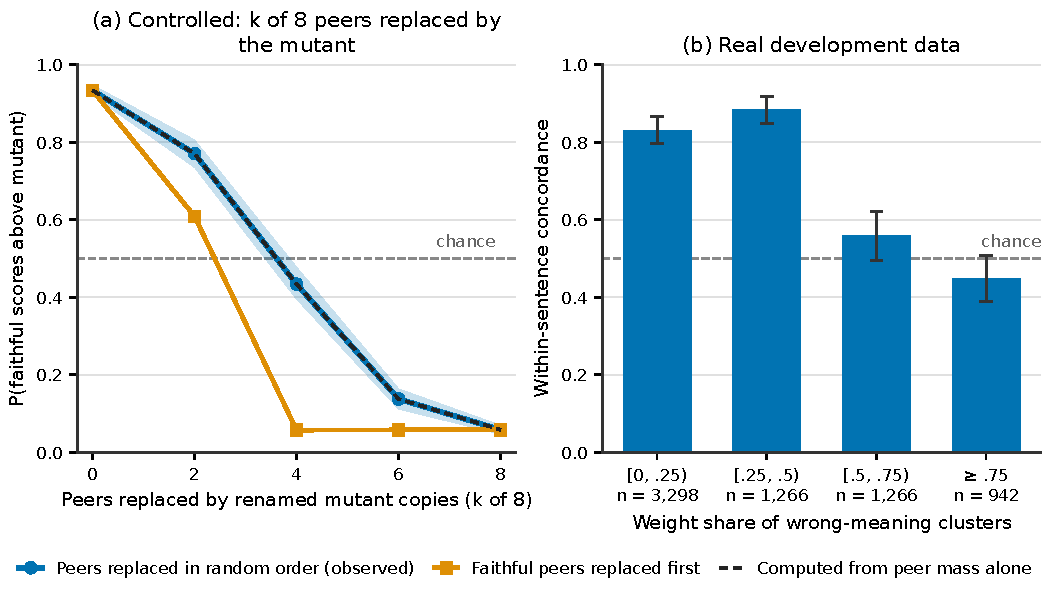
\includegraphics[width=\linewidth,height=0.85\textheight,keepaspectratio]{figures/fig8_v0.pdf}
\caption{The shared-bias boundary of directional consensus on the development set. (a) Controlled shared error: probability that the faithful formula outscores a mutant as k of its 8 peers are replaced by renamed copies of the mutant (560 items from 200 sentences, four operators; 95\% CIs for the random-order curve). The observed curve equals the curve computed from peer mass alone. (b) Real shared bias: within-sentence concordance over 6,772 faithful $\times$ unfaithful pairs, binned by the weight share of wrong-meaning clusters in the sentence (logistic slope $-$2.08 [$-$2.55, $-$1.61]).}
\label{fig:fig8}
\end{figure}

The text-anchored arbiter that was to repair part of this boundary, one solver-built world between the two largest clusters judged against the sentence by gemini-2.5-flash, was not run. The run budget returned HTTP 403 for every call; the key was polled every 10 minutes for an hour. All 783 constructed and 619 real arbiter prompts are saved, and re-asking them would cost about \$0.10.

\subsubsection{Search placebos}

Three placebos asked whether the alignment search manufactures agreement or whether DC mostly measures sentence difficulty (Table 35). Across 1,000 candidates paired with four arity-matched outputs from other sentences, 16.2\% were equivalent under a bijection. These are shape-isomorphic formulas such as ``All A are B'' against ``All C are D'', which no name-free comparison can separate. Partial maps added no spurious equivalence on non-isomorphic pairs; granularity definitions added 11.9\% (15.3\% for formulas of at most three atoms, 0\% at seven or more). When labels were shuffled within sentences 200 times, DC kept a panel AUROC of 0.73 against a true 0.77, and 0.70 against 0.82 under solver labels. Most of DC's item-level AUROC is therefore between-sentence structure: sentences whose outputs agree are more often translated correctly. The signature showed the same pattern at 0.648 (round 2, part 4).

\begin{table}[H]
\centering
\small
\setlength{\tabcolsep}{3pt}
\caption*{\textbf{Table 35.} Search placebos on the development set. (a) spurious equivalence with peers from other sentences; (c) within-sentence AUROC over faithful $\times$ unfaithful pairs of the same sentence; (d) share of within-sentence equivalences that are not equivalent under the lexically anchored map. \textit{[Source: development stress test, \texorpdfstring{\textup{\nolinkurl{gen_art_experiment_4}}}{gen art experiment 4}, iteration 2]}}
\begin{tabular}{>{\raggedright\arraybackslash}p{0.592\linewidth}>{\raggedright\arraybackslash}p{0.372\linewidth}}
\toprule
\textbf{Placebo} & \textbf{Result} \\
\midrule
{}(a) cross-sentence pairs equivalent under a bijection (shape-isomorphic) & 16.2\% of 3,982 pairs \\
{}(a) spurious equivalence added by partial maps / granularity definitions, non-isomorphic pairs & 0.0\% / 11.9\% \\
{}(b) within-sentence label shuffle, AUROC panel / solver & 0.73 (true 0.77) / 0.70 (true 0.82) \\
{}(c) within-sentence AUROC, panel (122 pairs): DC / without granularity / majority / binary Dawid-Skene model / cheap judge & 0.56 [0.41, 0.73] / 0.59 / 0.69 / 0.58 / 0.75 \\
{}(c) within-sentence AUROC, solver (6,772 pairs): same order & 0.74 / 0.75 / 0.76 / 0.76 / 0.68 \\
{}(d) manufactured equivalences overall & 1.9\% \\
{}(d) manufactured equivalences, unfaithful vs faithful items, panel / solver & 3.7\% vs 2.1\% / 4.3\% vs 1.3\% \\
\bottomrule
\end{tabular}
\end{table}

Forcing the lexical map throughout costs 0.16 AUROC (Table 28), so manufactured agreement is a minor channel, although it is enriched among unfaithful items as predicted.

\subsubsection{Which component carries the signal, and error typing}

We call a sequence of ablations that adds one component at a time an \emph{ablation ladder}. The ablation ladder in Table 36 starts from bijection-only agreement. Partial maps carry the whole gain over bijection-only agreement (+0.128 [0.081, 0.178]); granularity definitions and Dawid-Skene model weights are neutral. The largest per-type lift from partial maps fell on $\forall$/$\exists$ and implication-direction errors, not on added conditions, so the mechanism prediction that direction would lift added conditions failed.

\begin{table}[H]
\centering
\small
\setlength{\tabcolsep}{3pt}
\caption*{\textbf{Table 36.} Ablation ladder on the development panel items, and error-type naming. \textit{[Source: development stress test, \texorpdfstring{\textup{\nolinkurl{gen_art_experiment_4}}}{gen art experiment 4}, iteration 2]}}
\begin{tabular}{>{\raggedright\arraybackslash}p{0.335\linewidth}>{\raggedright\arraybackslash}p{0.293\linewidth}>{\raggedright\arraybackslash}p{0.192\linewidth}>{\raggedright\arraybackslash}p{0.119\linewidth}}
\toprule
\textbf{Step} & \textbf{panel AUROC} & \textbf{$\Delta$ vs previous [95\% CI]} & \textbf{solver AUROC} \\
\midrule
{}level-1 equivalence share & 0.636 & n/a & 0.717 \\
{}+ partial maps & 0.763 & +0.128 [0.081, 0.178] & 0.818 \\
{}+ granularity definitions & 0.758 & $-$0.006 [$-$0.022, 0.010] & 0.799 \\
{}+ Dawid-Skene model weights (= DC) & 0.769 & +0.011 [$-$0.005, 0.027] & 0.815 \\
{}typing, real panel-unfaithful items, weighted top-1 & DC 0.213; majority class 0.257; error-typed judge 0.407 on the same items &  &  \\
{}typing, constructed mutants (contract rules) & accuracy 0.26, macro-F1 0.44 &  &  \\
\bottomrule
\end{tabular}
\end{table}

On constructed mutants $\forall$/$\exists$ was typed correctly 98\% of the time, while negation and implication were rarely named, because granularity definitions absorb negation and clusters built by transitive closure can place a mutant inside the mode.

\subsubsection{Completing the round-2 record}

The review asked for the within-sentence comparisons behind the round-2 dropped-condition and implication-direction claims to be recomputed with the cheap judge scored on every pair and with the round-trip and agreement baselines added. The artifact rebuilt the round-2 partnered set exactly (246 errors with a faithful partner; 36 dropped-condition and 24 implication-direction errors; 21 fallback golds) and scored every available metric on it (Table 37). Detection is the weighted probability that a faithful partner outscores the error, ties counted one half. Two things change the round-2 reading. The cheap judge scored on 34 of the 36 dropped-condition errors detects them at 0.577, not the 0.618 of its 21-item subset, and on 21 of the 24 implication-direction errors at 0.576, not 0.770. No agreement metric reaches the repaired signature's 0.853 and 0.866 (Table 149) on these two classes; round-trip cosine, scored where round 2 ran it, reaches 0.711 and 0.923 on 21 and 11 errors.

\begin{landscape}
{\footnotesize
\setlength{\tabcolsep}{3pt}
\begin{longtable}{>{\raggedright\arraybackslash}p{0.085\linewidth}>{\raggedright\arraybackslash}p{0.052\linewidth}>{\raggedright\arraybackslash}p{0.100\linewidth}>{\raggedright\arraybackslash}p{0.100\linewidth}>{\raggedright\arraybackslash}p{0.081\linewidth}>{\raggedright\arraybackslash}p{0.081\linewidth}>{\raggedright\arraybackslash}p{0.109\linewidth}>{\raggedright\arraybackslash}p{0.081\linewidth}>{\raggedright\arraybackslash}p{0.109\linewidth}>{\raggedright\arraybackslash}p{0.100\linewidth}}
\caption*{\textbf{Table 37.} Within-sentence detection on the round-2 partnered set, by the panel's primary error type (n errors; n scored in parentheses where coverage is partial; round-trip scores exist only where the round-2 confirmation ran back-translation). \textit{[Source: development stress test, \texorpdfstring{\textup{\nolinkurl{gen_art_experiment_4}}}{gen art experiment 4}, iteration 2]}}\\
\toprule
\textbf{Error type (n)} & \textbf{cheap judge} & \textbf{round-trip NLI} & \textbf{round-trip cosine} & \textbf{majority} & \textbf{one-coin model} & \textbf{binary Dawid-Skene model} & \textbf{DC (frozen)} & \textbf{DC without granularity} & \textbf{vocabulary conformity} \\
\midrule
\endfirsthead
\multicolumn{10}{l}{\textit{(continued)}}\\
\toprule
\textbf{Error type (n)} & \textbf{cheap judge} & \textbf{round-trip NLI} & \textbf{round-trip cosine} & \textbf{majority} & \textbf{one-coin model} & \textbf{binary Dawid-Skene model} & \textbf{DC (frozen)} & \textbf{DC without granularity} & \textbf{vocabulary conformity} \\
\midrule
\endhead
\bottomrule
\endlastfoot
{}added condition (65) & 0.587 (59) & 0.651 (25) & 0.832 (25) & 0.630 & 0.641 & 0.597 & 0.653 (65) & 0.712 & 0.549 \\
{}dropped condition (36) & 0.577 (34) & 0.702 (21) & 0.711 (21) & 0.563 & 0.485 & 0.488 & 0.437 (36) & 0.583 & 0.521 \\
{}$\forall$/$\exists$ choice (56) & 0.820 (53) & 0.691 (19) & 0.670 (19) & 0.806 & 0.851 & 0.883 & 0.719 (56) & 0.734 & 0.666 \\
{}implication direction (24) & 0.576 (21) & 0.597 (11) & 0.923 (11) & 0.641 & 0.715 & 0.670 & 0.578 (24) & 0.712 & 0.353 \\
{}quantifier scope (12) & 0.923 (11) & 0.635 (6) & 0.665 (6) & 0.721 & 0.724 & 0.795 & 0.597 (12) & 0.602 & 0.644 \\
{}conjunction / disjunction (10) & 0.886 (10) & 1.000 (6) & 1.000 (6) & 0.718 & 0.833 & 0.833 & 0.734 (10) & 0.718 & 0.424 \\
{}negation / polarity (5) & 0.963 (5) & 1.000 (3) & 0.575 (3) & 0.487 & 0.406 & 0.406 & 0.603 (5) & 0.603 & 0.295 \\
{}predicted visible, pooled (188) & 0.670 (173) & 0.674 (80) & 0.739 (80) & 0.670 & 0.679 & 0.668 & 0.623 (188) & 0.691 & 0.556 \\
{}predicted blind, pooled (23) & 0.923 (22) & 0.776 (12) & 0.794 (12) & 0.684 & 0.725 & 0.801 & 0.549 (23) & 0.545 & 0.564 \\
\end{longtable}
}
\end{landscape}

The agreement metrics other than DC were scored on the same items as the cheap judge. Argument-swap (2) and cardinality (1) rows are in \texttt{results/\allowbreak{}m6\_\allowbreak{}\allowbreak{}within\_\allowbreak{}\allowbreak{}sentence.json} and are too small to read.

The artifact also settled the citation question the review raised about the relabelling study [4]. The figures in this report's framing are from version 2 of arXiv:2606.02837; version 1, whose abstract the hypothesis quotes, gives different ones (Table 38).

\begin{table}[H]
\centering
\small
\setlength{\tabcolsep}{3pt}
\caption*{\textbf{Table 38.} Figures reported by the two versions of arXiv:2606.02837. \textit{[Source: development stress test, \texorpdfstring{\textup{\nolinkurl{gen_art_experiment_4}}}{gen art experiment 4}, iteration 2]}}
\begin{tabular}{>{\raggedright\arraybackslash}p{0.371\linewidth}>{\raggedright\arraybackslash}p{0.255\linewidth}>{\raggedright\arraybackslash}p{0.326\linewidth}}
\toprule
\textbf{Quantity} & \textbf{v1} & \textbf{v2 (current)} \\
\midrule
{}incorrect FOL, FOLIO / MALLS & 39\% / 36\% & 42.5\% / 42\% \\
{}ambiguous NL, FOLIO / MALLS & 16.4\% / 48\% & 17.8\% / 51\% \\
{}guided review needed to reach 90\% dataset accuracy & ``fewer than 24\%'' of instances & ``fewer than 20\%'' (unguided: over 76\%) \\
\bottomrule
\end{tabular}
\end{table}

\subsubsection{The shipped gold as a tenth peer}

Scoring the shipped gold formula against the nine system outputs gives a gold-free wrong-gold flag. Against the panel's gold verdict on 700 development golds (43\% wrong), DC reached 0.837 [0.809, 0.864] with coverage 0.966 (Table 39). The signature had scored 0.673 on the same task (Table 150). Stacked with a judge run on the gold, DC adds +0.070 over the cheap judge and +0.048 over the error-typed judge. The nearest published neighbour is the LLM-guided relabelling framework of Brunello et al. [4], which prioritises items for human review and reports reaching 90\% dataset accuracy after reviewing fewer than 20\% of instances; no head-to-head was run against it. Label-error detection with LLM ensembles in general NLP benchmarks [44] is the other close relative.

\begin{table}[H]
\centering
\small
\setlength{\tabcolsep}{3pt}
\caption*{\textbf{Table 39.} Wrong-gold flag from DC with the gold as a tenth peer (700 development golds, panel gold verdicts). \textit{[Source: development stress test, \texorpdfstring{\textup{\nolinkurl{gen_art_experiment_4}}}{gen art experiment 4}, iteration 2]}}
\begin{tabular}{>{\raggedright\arraybackslash}p{0.373\linewidth}>{\raggedright\arraybackslash}p{0.206\linewidth}>{\raggedright\arraybackslash}p{0.372\linewidth}}
\toprule
\textbf{Population or stack} & \textbf{AUROC [95\% CI]} & \textbf{note} \\
\midrule
{}pooled & 0.837 [0.809, 0.864] & 43\% wrong gold \\
{}ProverQA & 0.891 & precision@25 0.76 at a 17.5\% base rate \\
{}MALLS & 0.783 &  \\
{}FOLIO & 0.733 &  \\
{}cheap judge on the gold $\rightarrow$ + DC & 0.825 $\rightarrow$ 0.896 & +0.070 [0.045, 0.096] \\
{}error-typed judge on the gold $\rightarrow$ + DC & 0.841 $\rightarrow$ 0.889 & +0.048 [0.028, 0.070] \\
\bottomrule
\end{tabular}
\end{table}

\subsubsection{Complexity, system level and cost}

By tercile on the development panel items, DC scored 0.767, 0.772 and 0.764, flat; binary Dawid-Skene model 0.754, 0.825 and 0.777; the cheap judge 0.798, 0.671 and 0.779. By number of conditions (0, 1, 2, $\geq$3), DC scored 0.865, 0.760, 0.638 and 0.838 against the judge's 0.906, 0.713, 0.707 and 0.806. Under solver labels the variant without granularity definitions beat the judge in every tercile (top tercile 0.812 against 0.719). Kendall $\tau$ with panel system accuracy over nine systems was 0.67 for DC, 0.78 for majority clustering and 0.72 for the judge; nine systems make these descriptive. DC costs no API call. Mean pair time was 0.13 s when a bijection decided the pair, 0.18 s for partial maps and 0.07 s for granularity definitions, with p95 at most 0.76 s. Timeouts were 0.09\%, unknown relations 0.12\% and engine errors 0.05\%, all counted as unknown. Relations were decided by unbounded proof 39.5k times, by fingerprint refutation 27.8k times and by bounded grounding alone 14 times.

\subsubsection{Pre-registered verdicts}

Table 40 gives every pre-registered prediction of the artifact and its outcome: 9 passed, 10 failed and 1 was not run. The recount in \texttt{checks/\allowbreak{}verify\_\allowbreak{}\allowbreak{}iter2.py} reads the same 9/10/1 split from \texttt{results/\allowbreak{}verdicts.json}.

{\small
\setlength{\tabcolsep}{3pt}
\begin{longtable}{>{\raggedright\arraybackslash}p{0.433\linewidth}>{\raggedright\arraybackslash}p{0.140\linewidth}>{\raggedright\arraybackslash}p{0.378\linewidth}}
\caption*{\textbf{Table 40.} Pre-registered predictions of the development stress test. \textit{[Source: development stress test, \texorpdfstring{\textup{\nolinkurl{gen_art_experiment_4}}}{gen art experiment 4}, iteration 2]}}\\
\toprule
\textbf{Prediction} & \textbf{Verdict} & \textbf{Key number} \\
\midrule
\endfirsthead
\multicolumn{3}{l}{\textit{(continued)}}\\
\toprule
\textbf{Prediction} & \textbf{Verdict} & \textbf{Key number} \\
\midrule
\endhead
\bottomrule
\endlastfoot
{}DC arm gap below 0.02 (vocabulary invariance) & pass & 0.0015 \\
{}DC on the crossed arm $\geq$ 0.85 & fail & 0.805 (without granularity definitions 0.999) \\
{}vocabulary-conformity arm gap $>$ 0.2 & fail & about 0.01; ill-posed, since within an arm faithful and mutant share vocabulary \\
{}vocabulary conformity on the crossed arm $<$ 0.5 & pass & 0.176 \\
{}automorphic mutants at chance & pass & 0.50 (n = 20) \\
{}granularity definitions absorb dropped conjuncts & pass & detection 0.68 vs 0.98 \\
{}DC adds over [judge, parse, vocabulary conformity], panel & fail & +0.015 [$-$0.009, 0.040] \\
{}rewrite false alarms at $\delta$ = 0.10 $\leq$ 0.05, every kind & pass & maximum 0.018 (contrapositive) \\
{}renaming false alarms at $\delta$ = 0 equal to 0 & fail & 0.001 (role tie-break) \\
{}no contamination shift & fail & +0.0023 [0.0001, 0.0055] against the judge's +0.096 \\
{}dose curve (detection $\geq$ 0.9 up to k = 2) & fail & only k = 2 misses (0.77) \\
{}arbiter improves on DC & not run & run budget exhausted \\
{}real shared-bias slope $<$ 0 & pass & $-$2.08 [$-$2.55, $-$1.61] \\
{}spurious cross-sentence equivalence $\leq$ 2\% & fail & partial maps 0.0\%, granularity 11.9\% \\
{}within-sentence shuffle near 0.5 & fail & 0.73 \\
{}manufactured agreement enriched among unfaithful & pass & panel 3.7\% vs 2.1\% \\
{}largest ladder lift on added conditions & fail & $\forall$/$\exists$ and implication direction \\
{}typing above the majority class & fail & 0.213 vs 0.257 \\
{}round-2 partnered counts reproduced (36 / 24) & pass & exact \\
{}wrong-gold flag AUROC $>$ 0.5 & pass & 0.837 [0.809, 0.864] \\
\end{longtable}
}

The artifact proposed four amendments for the confirmation and applied none of them to its own frozen code: freeze the variant without granularity definitions (or forbid single negated-literal definitions); break role ties with a name-free structural key; type errors by the direct relation to the modal representative; and make within-sentence detection co-primary. It reported its reading plainly. As frozen, DC is exactly name-free and nearly contamination-proof and is a strong wrong-gold flag, but it is not better than simple bijection-plus-partial-map cluster agreement, its granularity layer manufactures agreement, most of its AUROC separates sentences, and it adds nothing over majority clustering.

\subsection{Freeze-then-confirm on fresh sentences (\texorpdfstring{\textup{\nolinkurl{gen_art_experiment_3}}}{gen art experiment 3})}

This subsection reports the artifact \texorpdfstring{\textup{\nolinkurl{gen_art_experiment_3}}}{gen art experiment 3}, the iteration's confirmation.

\subsubsection{The freeze}

The confirmation artifact implemented DC independently from the same contract (16 unit tests pass; the vendored parser and solver tests pass 29 of 29) and chose its configuration on the development set from a 12-configuration grid. The rule was fixed in advance: maximise the mean of panel and solver AUROC, with ties within 0.005 going to the simpler configuration. Table 41 gives the grid. The selected configuration drops granularity definitions, keeps UNALIGNABLE peers in the denominator and uses Dawid-Skene model weights. Granularity definitions produced equivalences that only they could produce on 5.8\% of pairs and broke transitivity of equivalence on 0.36\% of cluster triples; without them both rates are near zero. Halving the alignment caps changed nothing. The receipt was written before any fresh label existed, and \texttt{results/\allowbreak{}integrity.json} confirms that no \texttt{dc/\allowbreak{}} file changed afterwards.

{\footnotesize
\setlength{\tabcolsep}{3pt}
\begin{longtable}{>{\raggedright\arraybackslash}p{0.184\linewidth}>{\raggedright\arraybackslash}p{0.073\linewidth}>{\raggedright\arraybackslash}p{0.073\linewidth}>{\raggedright\arraybackslash}p{0.059\linewidth}>{\raggedright\arraybackslash}p{0.115\linewidth}>{\raggedright\arraybackslash}p{0.170\linewidth}>{\raggedright\arraybackslash}p{0.226\linewidth}}
\caption*{\textbf{Table 41.} Development grid used for the freeze (609 panel items, 5,846 solver rows). Rows name the three choices: granularity definitions on or off, UNALIGNABLE peers in or out of the denominator, and Dawid-Skene model or uniform weights; the last field gives the alignment caps (0.5 = halved). \textit{[Source: fresh confirmation, \texorpdfstring{\textup{\nolinkurl{gen_art_experiment_3}}}{gen art experiment 3}, iteration 2]}}\\
\toprule
\textbf{Configuration} & \textbf{AUROC P} & \textbf{AUROC S} & \textbf{mean} & \textbf{coverage} & \textbf{equivalences only via partial or granularity maps} & \textbf{non-transitivity} \\
\midrule
\endfirsthead
\multicolumn{7}{l}{\textit{(continued)}}\\
\toprule
\textbf{Configuration} & \textbf{AUROC P} & \textbf{AUROC S} & \textbf{mean} & \textbf{coverage} & \textbf{equivalences only via partial or granularity maps} & \textbf{non-transitivity} \\
\midrule
\endhead
\bottomrule
\endlastfoot
{}granularity on, unalignable in, DS, caps 1 & 0.768 & 0.826 & 0.797 & 0.952 & 0.058 & 0.0036 \\
{}granularity on, unalignable in, uniform, caps 1 & 0.760 & 0.813 & 0.786 & 0.952 & 0.058 & 0.0036 \\
{}granularity on, unalignable out, DS, caps 1 & 0.782 & 0.814 & 0.798 & 0.930 & 0.058 & 0.0036 \\
{}granularity on, unalignable out, uniform, caps 1 & 0.774 & 0.797 & 0.785 & 0.930 & 0.058 & 0.0036 \\
{}\textbf{granularity off, unalignable in, DS, caps 1 (frozen)} & 0.777 & 0.855 & 0.816 & 0.952 & 0.001 & 0.0000 \\
{}granularity off, unalignable in, uniform, caps 1 & 0.771 & 0.841 & 0.806 & 0.952 & 0.001 & 0.0000 \\
{}granularity off, unalignable out, DS, caps 1 & 0.791 & 0.843 & 0.817 & 0.930 & 0.001 & 0.0000 \\
{}granularity off, unalignable out, uniform, caps 1 & 0.784 & 0.826 & 0.805 & 0.930 & 0.001 & 0.0000 \\
{}granularity on, unalignable in, DS, caps 0.5 & 0.768 & 0.826 & 0.797 & 0.952 & 0.058 & 0.0036 \\
{}granularity on, unalignable in, uniform, caps 0.5 & 0.760 & 0.813 & 0.786 & 0.952 & 0.058 & 0.0036 \\
{}granularity on, unalignable out, DS, caps 0.5 & 0.782 & 0.814 & 0.798 & 0.930 & 0.058 & 0.0036 \\
{}granularity on, unalignable out, uniform, caps 0.5 & 0.774 & 0.797 & 0.785 & 0.930 & 0.058 & 0.0036 \\
\end{longtable}
}

The frozen configuration is 0.001 below the configuration that leaves UNALIGNABLE peers out of the denominator on the mean and was chosen under the tie rule as the simpler one. Two code fixes were made before the freeze and recorded: the 50\% mapped-share rule of partial maps was made symmetric after a unit test found 17 of 50 development pairs asymmetric, and the one-coin Dawid-Skene model lost its ``none of the clusters'' state, which had produced degenerate optima. Error typing was left weak on purpose: on development data 68\% of typed errors came out ``other'', and the literal-flip negation rule gave no gain and was frozen off.

\subsubsection{The fresh set and its labels}

The fresh set holds 450 sentences drawn with a fixed seed from the eligible pool of Section 3.6, with 1,204 excluded strings and 237 excluded stories; overlap with the development, screen and contamination sentences was asserted zero at both the string and story level. Half of the sentences fall in the top complexity tercile (Table 42). The nine systems of Section 3.6 translated every sentence with the frozen prompt (4,050 greedy candidates, 222 unparseable and kept), and gpt-4.1-mini and llama-3.1-8b each drew 5 samples at T = 0.8 (4,500 samples).

\begin{table}[H]
\centering
\small
\setlength{\tabcolsep}{3pt}
\caption*{\textbf{Table 42.} Fresh sentences by corpus and complexity tercile (every quota met; available pool in parentheses). \textit{[Source: fresh confirmation, \texorpdfstring{\textup{\nolinkurl{gen_art_experiment_3}}}{gen art experiment 3}, iteration 2]}}
\begin{tabular}{>{\raggedright\arraybackslash}p{0.392\linewidth}>{\raggedright\arraybackslash}p{0.153\linewidth}>{\raggedright\arraybackslash}p{0.153\linewidth}>{\raggedright\arraybackslash}p{0.117\linewidth}>{\raggedright\arraybackslash}p{0.112\linewidth}}
\toprule
\textbf{Corpus} & \textbf{bottom} & \textbf{middle} & \textbf{top} & \textbf{total} \\
\midrule
{}MALLS-v0.1-test & 34 (43) & 51 (110) & 85 (591) & 170 \\
{}FOLIO-v2-train, disjoint stories & 30 (411) & 45 (95) & 75 (147) & 150 \\
{}ProverQA-dev medium/hard & 26 (493) & 39 (968) & 65 (283) & 130 \\
{}total & 90 & 135 & 225 & 450 \\
\bottomrule
\end{tabular}
\end{table}

Labels followed the round-1 protocol. A cascaded panel audited all 450 shipped golds; its cascade was changed for cost (glm-4.6 on every gold, claude-haiku-4.5 where glm rejected, grok-4.3 as tie-break) and agreed with the full three-member majority on 45 of 45 golds in a 10\% subset. Solver labels are lexical-free Z3 equivalence to the audited gold (3,720 greedy rows). The blinded three-model panel adjudicated 272 sampled items; 16 lost their tie-break when the key ran out and were excluded and counted, leaving 256. The sampler took one member of the modal cluster and one minority member from each of 130 sentences, plus 12 unparseable items, and weights were post-stratified and then raked over the generating system (Kish effective n 202). Table 43 gives the label quality. The rates reproduce the development set's: wrong gold on 45.8\% of fresh golds overall, 43.8\% of solver-non-equivalent panel items faithful (43.9\% in Section 3.6), and solver-panel agreement of 68.9\% (67.6\%).

\begin{table}[H]
\centering
\small
\setlength{\tabcolsep}{3pt}
\caption*{\textbf{Table 43.} Label quality on the fresh set. \textit{[Source: fresh confirmation, \texorpdfstring{\textup{\nolinkurl{gen_art_experiment_3}}}{gen art experiment 3}, iteration 2]}}
\begin{tabular}{>{\raggedright\arraybackslash}p{0.572\linewidth}>{\raggedright\arraybackslash}p{0.393\linewidth}}
\toprule
\textbf{Quantity} & \textbf{Value} \\
\midrule
{}wrong shipped gold, MALLS (170) / FOLIO (150) / ProverQA (130) & 0.553 [0.482, 0.629] / 0.620 [0.540, 0.700] / 0.146 [0.092, 0.208] \\
{}gold corrections accepted / flagged but uncorrected (unknown solver label) & 193 / 13 \\
{}panel-faithful share among solver-non-equivalent panel items (n = 168, weighted) & 0.438 \\
{}panel-unfaithful share among solver-equivalent panel items (n = 77) & 0.081 \\
{}solver-panel agreement (weighted) & 0.689 \\
{}calibration gate: claude-haiku-4.5 / grok-4.3 / glm-4.6 & 0.90 / 0.90 / 0.85 \\
{}Fleiss $\kappa$, full-panel subset of the adjudication (n = 24) / of the gold audit (n = 45) & 0.538 / 0.466 \\
{}panel weights: frame n, items, floor-capped, Kish n, max/min ratio & 3,933; 256; 148; 202; 6.0 \\
\bottomrule
\end{tabular}
\end{table}

\subsubsection{Main result}

Table 44 is the confirmation table. Under panel labels DC scores 0.827 and ties the frozen round-2 latent-class variants (0.830 to 0.836); scoring unparseable outputs 0 rather than 0.5 raises it to 0.853, because the panel sample includes 12 unparseable items. Under solver labels DC is the best row (0.874). The cheap judge is 0.036 below DC on panel labels and 0.147 below on solver labels. The user's structural metrics and parse rate are near chance, as in round 2. The local round-trip substitutes score 0.784 and 0.752 on panel items and 0.619 and 0.657 under solver labels; on the 18 panel items generated by Qwen models they scored 0.968 (round-trip NLI) against 0.766 on the others, so the Qwen3-8B substitute favours its own family. The frozen configuration transferred: development 0.777 / 0.855, fresh 0.827 / 0.874.

{\footnotesize
\setlength{\tabcolsep}{3pt}
\begin{longtable}{>{\raggedright\arraybackslash}p{0.357\linewidth}>{\raggedright\arraybackslash}p{0.145\linewidth}>{\raggedright\arraybackslash}p{0.051\linewidth}>{\raggedright\arraybackslash}p{0.145\linewidth}>{\raggedright\arraybackslash}p{0.076\linewidth}>{\raggedright\arraybackslash}p{0.138\linewidth}}
\caption*{\textbf{Table 44.} Fresh confirmation: AUROC under panel labels (256 adjudicated items, raked weights) and audited-solver labels (3,720 rows unless stated). L = local Qwen3-8B substitute for a gemini baseline. \textit{[Source: fresh confirmation, \texorpdfstring{\textup{\nolinkurl{gen_art_experiment_3}}}{gen art experiment 3}, iteration 2]}}\\
\toprule
\textbf{Metric} & \textbf{AUROC P [95\% CI]} & \textbf{n P} & \textbf{AUROC S [95\% CI]} & \textbf{n S} & \textbf{coverage} \\
\midrule
\endfirsthead
\multicolumn{6}{l}{\textit{(continued)}}\\
\toprule
\textbf{Metric} & \textbf{AUROC P [95\% CI]} & \textbf{n P} & \textbf{AUROC S [95\% CI]} & \textbf{n S} & \textbf{coverage} \\
\midrule
\endhead
\bottomrule
\endlastfoot
{}DC, unparseable scored 0 & 0.853 [0.798, 0.898] & 256 & 0.874 [0.849, 0.897] & 3,720 & 1.000 \\
{}sampling self-consistency (2 systems) & 0.843 [0.777, 0.904] & 143 & 0.784 [0.753, 0.813] & 823 & 0.993 \\
{}DC with own samples as peers (2 systems) & 0.842 [0.775, 0.903] & 143 & 0.784 [0.754, 0.814] & 823 & 0.993 \\
{}latent class, two-population design (Hui-Walter) & 0.836 [0.778, 0.887] & 256 & 0.852 [0.824, 0.877] & 3,720 & 0.984 \\
{}latent class, one-coin model & 0.834 [0.776, 0.885] & 256 & 0.850 [0.823, 0.876] & 3,720 & 0.984 \\
{}binary Dawid-Skene model & 0.830 [0.773, 0.878] & 256 & 0.865 [0.840, 0.889] & 3,720 & 0.984 \\
{}\textbf{DC (frozen, pre-registered)} & 0.827 [0.770, 0.877] & 256 & 0.874 [0.849, 0.897] & 3,720 & 1.000 \\
{}majority clustering & 0.797 [0.737, 0.850] & 256 & 0.859 [0.833, 0.883] & 3,720 & 0.984 \\
{}cheap judge (gemini-2.5-flash) & 0.791 [0.726, 0.843] & 256 & 0.727 [0.698, 0.755] & 3,720 & 1.000 \\
{}round-trip NLI (L) & 0.784 [0.724, 0.835] & 256 & 0.619 [0.546, 0.687] & 260 & 1.000 \\
{}round-trip cosine (L) & 0.752 [0.686, 0.817] & 256 & 0.657 [0.587, 0.730] & 260 & 1.000 \\
{}vocabulary conformity & 0.674 [0.598, 0.746] & 256 & 0.791 [0.764, 0.815] & 3,720 & 1.000 \\
{}error-typed judge (L) & 0.659 [0.611, 0.710] & 256 & 0.593 [0.557, 0.631] & 260 & 1.000 \\
{}structural (user pilot) & 0.554 [0.522, 0.590] & 256 & 0.503 [0.500, 0.505] & 3,720 & 1.000 \\
{}parse rate & 0.549 [0.518, 0.584] & 256 & 0.500 [0.500, 0.500] & 3,720 & 1.000 \\
{}net strength profile & 0.415 [0.358, 0.467] & 245 & 0.464 [0.449, 0.480] & 3,720 & 1.000 \\
\end{longtable}
}

The ``coverage'' column counts items with a score; DC gives 0.5 to 222 unparseable outputs and 1 item with fewer than two covered peers, for a covered share of 0.945 over all 4,050 greedy rows. The net strength profile, the directional part of the hypothesis, ranks candidates below chance. Figure~\ref{fig:fig7} plots Table 44 under both label families.

\begin{figure}[!htbp]
\centering
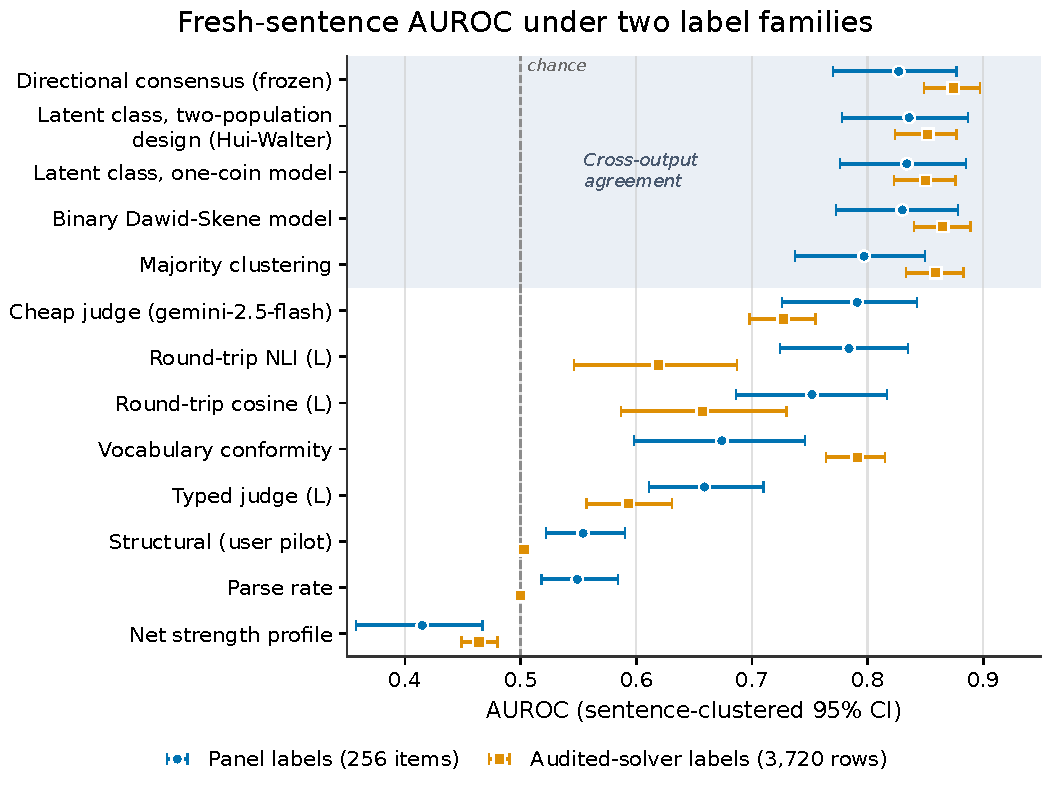
\includegraphics[width=\linewidth,height=0.85\textheight,keepaspectratio]{figures/fig7_v0.pdf}
\caption{Fresh confirmation set (450 new sentences $\times$ 9 systems): AUROC with sentence-clustered 95\% CIs under panel labels (256 adjudicated items, raked weights) and audited-solver labels (3,720 rows; 260 rows for the local round-trip and typed-judge substitutes, marked L). Cross-output agreement (directional consensus and the latent-class variants) leads under both labels; the cheap judge drops from 0.791 to 0.727 when the labels switch to solver equivalence; parse rate and the user's structural metrics sit at chance; the directional strength profile ranks below chance.}
\label{fig:fig7}
\end{figure}

\subsubsection{The pre-registered tests}

Table 45 gives the four tests. The increment test passes under both labels, thinly on the panel (one-sided lower bound +0.005 with the local round-trip substitute in the base) and clearly against the purely API-scored base [judge, parse, structural] (+0.126 [0.066, 0.189]). A placebo that shuffles DC within corpus $\times$ tercile strata gives about zero. The neighbour test is label-dependent: DC beats majority clustering and the vocabulary-conformity control under both labels, but on panel labels it does not beat the binary Dawid-Skene model that round 2 already had ($-$0.003 [$-$0.024, 0.017]). The error-type test fails on every clause that could be evaluated; its within-sentence clause has only 7 pairs per class. The lone-output test fails because DC computed on a system's own samples is numerically the same score as sampling self-consistency.

{\small
\setlength{\tabcolsep}{3pt}
\begin{longtable}{>{\raggedright\arraybackslash}p{0.301\linewidth}>{\raggedright\arraybackslash}p{0.237\linewidth}>{\raggedright\arraybackslash}p{0.180\linewidth}>{\raggedright\arraybackslash}p{0.221\linewidth}}
\caption*{\textbf{Table 45.} Pre-registered tests on the fresh set (the error-type test on panel labels only). LB5 in the cells = one-sided 95\% lower bound. \textit{[Source: fresh confirmation, \texorpdfstring{\textup{\nolinkurl{gen_art_experiment_3}}}{gen art experiment 3}, iteration 2]}}\\
\toprule
\textbf{Test} & \textbf{Panel} & \textbf{Solver} & \textbf{Verdict} \\
\midrule
\endfirsthead
\multicolumn{4}{l}{\textit{(continued)}}\\
\toprule
\textbf{Test} & \textbf{Panel} & \textbf{Solver} & \textbf{Verdict} \\
\midrule
\endhead
\bottomrule
\endlastfoot
{}T1 $\Delta$AUROC(base + DC $-$ base), base [judge, parse, round-trip NLI (L), round-trip cosine (L), structural] & +0.033 [$-$0.001, 0.066], LB5 +0.005 & +0.118 [0.051, 0.192], LB5 +0.060 (panel frame, n = 245) & pass \\
{}T1 placebo, DC shuffled within strata & $-$0.003 [$-$0.016, 0.008] & $-$0.001 [$-$0.010, 0.007] & $\approx$ 0 as required \\
{}T1 sensitivity, base [judge, parse, structural] & +0.126 [0.066, 0.189] & +0.159 [0.129, 0.190] (all 3,720 rows) & n/a \\
{}T2 DC $-$ majority clustering (LB $>$ 0) & +0.030 [0.012, 0.049], LB5 +0.014 & +0.015 [0.005, 0.026], LB5 +0.007 &  \\
{}T2 DC $-$ binary Dawid-Skene model (point $>$ 0) & $-$0.003 [$-$0.024, 0.017], LB5 $-$0.021 & +0.009 [$-$0.000, 0.019], LB5 +0.001 &  \\
{}T2 DC $-$ vocabulary conformity (LB $>$ 0) & +0.152 [0.096, 0.209], LB5 +0.104 & +0.083 [0.066, 0.102], LB5 +0.069 &  \\
{}T2 overall & fail & pass & label-dependent \\
{}T3a weighted top-1 type & DC 0.122 vs majority class (added condition) 0.255 + 0.10; error-typed judge (L) 0.017 & panel only & fail \\
{}T3b recall $\geq$ 0.5 on added / dropped / $\forall$$\exists$ & 0.039 (n = 27) / 0.410 (n = 14) / 0.252 (n = 21) & n/a & fail \\
{}T3c within-sentence DC vs cheap judge & dropped: 1.000 vs 0.643 (7 pairs); implication: 1.000 vs 0.786 (7 pairs); underpowered & n/a & fail (underpowered) \\
{}T4 gpt-4.1-mini: DC\_\allowbreak{}self $-$ self-consistency; stack $\Delta$ & 0.000 (LB5 0.000); +0.015 (LB5 $-$0.062), n = 76 & $-$0.002 (LB5 $-$0.007); +0.089 (LB5 +0.054), n = 431 & fail \\
{}T4 llama-3.1-8b & $-$0.016 (LB5 $-$0.041); $-$0.042 (LB5 $-$0.103), n = 67 & +0.005 (LB5 $-$0.002); +0.125 (LB5 +0.081), n = 392 & fail \\
\end{longtable}
}

Under the pre-registered decision rule, the first branch requires the increment and neighbour tests to pass under both labels, so the claim is not supported as stated. The increment test passed, and the neighbour test failed only against binary Dawid-Skene model on panel labels while passing against the vocabulary control, so neither the ``vocabulary conformity'' branch nor the ``closed'' branch applies. The result stands as: cross-output agreement adds to the judge-plus-round-trip base on fresh sentences under both labels, and the directional machinery adds nothing detectable over the agreement scored by the binary Dawid-Skene model round 2 already had.

The increment test used a one-sided 95\% bound (the 5th bootstrap percentile), whereas round 2 judged its increments by the lower end of a two-sided 95\% interval (the 2.5th percentile). The iteration-2 review pointed this out (Section 6.8). Under round 2's rule the fresh panel increment, +0.033 [$-$0.001, 0.066], would fail; under the one-sided rule several round-2 increments that were reported as not confirmed, such as majority agreement's +0.028 [$-$0.002, 0.056], would roughly pass. The point estimates are about the same size in both populations (+0.019 to +0.028 held-out, +0.033 fresh).

The artifact's independent re-derivation (\texttt{results/\allowbreak{}rederive\_\allowbreak{}\allowbreak{}headline.json}) reproduced the six headline AUROCs exactly. Its separate logistic refit gave a panel increment of +0.029 with lower bound +0.0035 from 300 refit draws, and a solver increment on the panel frame of +0.131; both keep the sign and the verdict. With permuted labels DC's solver AUROC averaged 0.501, and the shuffled-DC placebo did not pass the increment test. Bounded and unbounded Z3 agreed on all 153 entailments that the unbounded check finished. Our own recomputation from the per-item rows (\texttt{checks/\allowbreak{}verify\_\allowbreak{}\allowbreak{}iter2.py}) reproduced every panel AUROC in Table 44 that we checked to three decimals (DC 0.827, unparseable-as-0 0.853, binary Dawid-Skene model 0.830, one-coin model 0.834, majority 0.797, cheap judge 0.791, vocabulary conformity 0.674). Our solver-label reconstruction found 3,475 of the 3,720 rows and gave values within 0.004 of the table (DC 0.876, cheap judge 0.729). The iteration-2 reviewer showed why 245 rows were missing: they are panel items whose label source is the panel but which also carry an audited solver status, and labelling every row by that status reproduces all 3,720 rows and the table's values exactly (DC 0.874, cheap judge 0.727). The same reviewer checked whether the panel sampler, which draws one modal and one minority member per sentence, inflates agreement AUROCs: under solver labels DC scores 0.850 on the panel frame against 0.874 on all rows, so it does not.

\subsubsection{Is DC re-deriving the solver label?}

DC and the solver label share the equivalence checker, so a high solver AUROC could be circular. Table 46 restricts the panel items to the 168 whose candidate the solver calls non-equivalent to the audited gold; solver labels call all of them wrong. DC still separates them at 0.776. Binary Dawid-Skene model (0.805) and the local round-trip NLI (0.799) do slightly better on the same items.

\begin{table}[H]
\centering
\small
\setlength{\tabcolsep}{3pt}
\caption*{\textbf{Table 46.} AUROC under panel labels inside the solver-non-equivalent panel items. \textit{[Source: fresh confirmation, \texorpdfstring{\textup{\nolinkurl{gen_art_experiment_3}}}{gen art experiment 3}, iteration 2]}}
\begin{tabular}{>{\raggedright\arraybackslash}p{0.301\linewidth}>{\raggedright\arraybackslash}p{0.367\linewidth}>{\raggedright\arraybackslash}p{0.284\linewidth}}
\toprule
\textbf{Metric} & \textbf{non-equivalent (n = 168)} & \textbf{no bijection to gold (n = 143)} \\
\midrule
{}DC & 0.776 [0.679, 0.858] & 0.771 [0.678, 0.855] \\
{}binary Dawid-Skene model & 0.805 [0.718, 0.878] & 0.796 [0.702, 0.871] \\
{}majority clustering & 0.752 [0.654, 0.836] & 0.744 [0.644, 0.829] \\
{}cheap judge & 0.738 [0.659, 0.816] & 0.744 [0.652, 0.822] \\
{}round-trip NLI (L) & 0.799 [0.738, 0.862] & 0.809 [0.733, 0.876] \\
{}vocabulary conformity & 0.554 [0.437, 0.671] & 0.585 [0.462, 0.714] \\
{}error-typed judge (L) & 0.647 [0.575, 0.713] & 0.633 [0.563, 0.706] \\
\bottomrule
\end{tabular}
\end{table}

\subsubsection{Which component carries the signal}

The fresh-set ablation ladder (Table 47) repeats the development finding from another angle. Bijection-only agreement with uniform weights already scores 0.801 / 0.864. Adding partial maps changes nothing here, adding granularity definitions lowers it, and Dawid-Skene model weights carry the step to DC's 0.827 / 0.874. A stack of DC with the strength-profile features scores 0.791, below DC alone. On this set, the weighting carries the gain and the directional alignment does not.

{\small
\setlength{\tabcolsep}{3pt}
\begin{longtable}{>{\raggedright\arraybackslash}p{0.677\linewidth}>{\raggedright\arraybackslash}p{0.137\linewidth}>{\raggedright\arraybackslash}p{0.137\linewidth}}
\caption*{\textbf{Table 47.} Ablation ladder on the fresh set, derived from one relation cache. \textit{[Source: fresh confirmation, \texorpdfstring{\textup{\nolinkurl{gen_art_experiment_3}}}{gen art experiment 3}, iteration 2]}}\\
\toprule
\textbf{Step} & \textbf{AUROC P} & \textbf{AUROC S} \\
\midrule
\endfirsthead
\multicolumn{3}{l}{\textit{(continued)}}\\
\toprule
\textbf{Step} & \textbf{AUROC P} & \textbf{AUROC S} \\
\midrule
\endhead
\bottomrule
\endlastfoot
{}bijection only, uniform & 0.801 & 0.864 \\
{}+ partial maps, uniform & 0.801 & 0.863 \\
{}+ granularity definitions, uniform & 0.791 & 0.839 \\
{}majority clustering & 0.797 & 0.859 \\
{}binary Dawid-Skene model & 0.830 & 0.865 \\
{}latent class, one-coin model & 0.834 & 0.850 \\
{}DC (frozen: partial maps, Dawid-Skene model weights) & 0.827 & 0.874 \\
{}DC, uniform weights & 0.801 & 0.863 \\
{}DC with granularity definitions, Dawid-Skene model & 0.820 & 0.859 \\
{}DC + strength profile (out-of-fold stack) & 0.791 & 0.867 \\
\end{longtable}
}

\subsubsection{Complexity}

Table 48 breaks the fresh items down by the four complexity features the user named. Under panel labels DC's lead over the cheap judge shrinks with complexity: by tercile the gap is +0.088, +0.107 and $-$0.028, a slope of $-$0.058 [$-$0.135, 0.022] that is not significant. DC is weakest on candidates with two or more quantifiers (0.659 against the judge's 0.778, n = 45), on nesting depth 4-5 and on sentences longer than 20 tokens, and strongest on sentences with three or more conditions (0.871 against 0.787, n = 124). Under solver labels DC is above the judge in every cell, but that arm is partly circular. These strata are connective-heavy, not exception-heavy; the exception-heavy test is Section 6.4. Figure~\ref{fig:fig9} draws the table.

{\footnotesize
\setlength{\tabcolsep}{3pt}
\begin{longtable}{>{\raggedright\arraybackslash}p{0.198\linewidth}>{\raggedright\arraybackslash}p{0.177\linewidth}>{\raggedright\arraybackslash}p{0.087\linewidth}>{\raggedright\arraybackslash}p{0.177\linewidth}>{\raggedright\arraybackslash}p{0.087\linewidth}>{\raggedright\arraybackslash}p{0.187\linewidth}}
\caption*{\textbf{Table 48.} Fresh-set AUROC by complexity stratum (panel P and solver S labels; n per cell). \textit{[Source: fresh confirmation, \texorpdfstring{\textup{\nolinkurl{gen_art_experiment_3}}}{gen art experiment 3}, iteration 2]}}\\
\toprule
\textbf{Stratum} & \textbf{DC P} & \textbf{cheap judge P} & \textbf{DC S} & \textbf{cheap judge S} & \textbf{binary Dawid-Skene model S} \\
\midrule
\endfirsthead
\multicolumn{6}{l}{\textit{(continued)}}\\
\toprule
\textbf{Stratum} & \textbf{DC P} & \textbf{cheap judge P} & \textbf{DC S} & \textbf{cheap judge S} & \textbf{binary Dawid-Skene model S} \\
\midrule
\endhead
\bottomrule
\endlastfoot
{}tokens $\leq$ 12 & 0.856 (80) & 0.764 & 0.885 (1,403) & 0.699 & 0.898 \\
{}tokens 13-20 & 0.824 (136) & 0.797 & 0.849 (1,808) & 0.746 & 0.824 \\
{}tokens $>$ 20 & 0.727 (40) & 0.810 & 0.881 (509) & 0.750 & 0.868 \\
{}quantifiers 0 & 0.923 (62) & 0.743 & 0.958 (932) & 0.814 & 0.943 \\
{}quantifiers 1 & 0.829 (149) & 0.820 & 0.841 (2,104) & 0.662 & 0.849 \\
{}quantifiers 2+ & 0.659 (45) & 0.778 & 0.847 (684) & 0.721 & 0.847 \\
{}nesting $\leq$ 3 & 0.875 (164) & 0.796 & 0.872 (2,364) & 0.737 & 0.861 \\
{}nesting 4-5 & 0.661 (68) & 0.732 & 0.849 (924) & 0.600 & 0.848 \\
{}nesting 6+ & 0.736 (24) & 0.780 & 0.817 (432) & 0.734 & 0.826 \\
{}conditions 0-1 & 0.768 (74) & 0.793 & 0.885 (1,142) & 0.718 & 0.897 \\
{}conditions 2 & 0.795 (58) & 0.806 & 0.884 (914) & 0.684 & 0.873 \\
{}conditions 3+ & 0.871 (124) & 0.787 & 0.860 (1,664) & 0.754 & 0.837 \\
{}tercile gap DC $-$ judge, bottom / middle / top & +0.088 / +0.107 / $-$0.028; slope $-$0.058 [$-$0.135, 0.022] &  & +0.167 / +0.166 / +0.118; slope $-$0.024 [$-$0.059, 0.009] &  &  \\
\end{longtable}
}

\begin{figure}[!htbp]
\centering
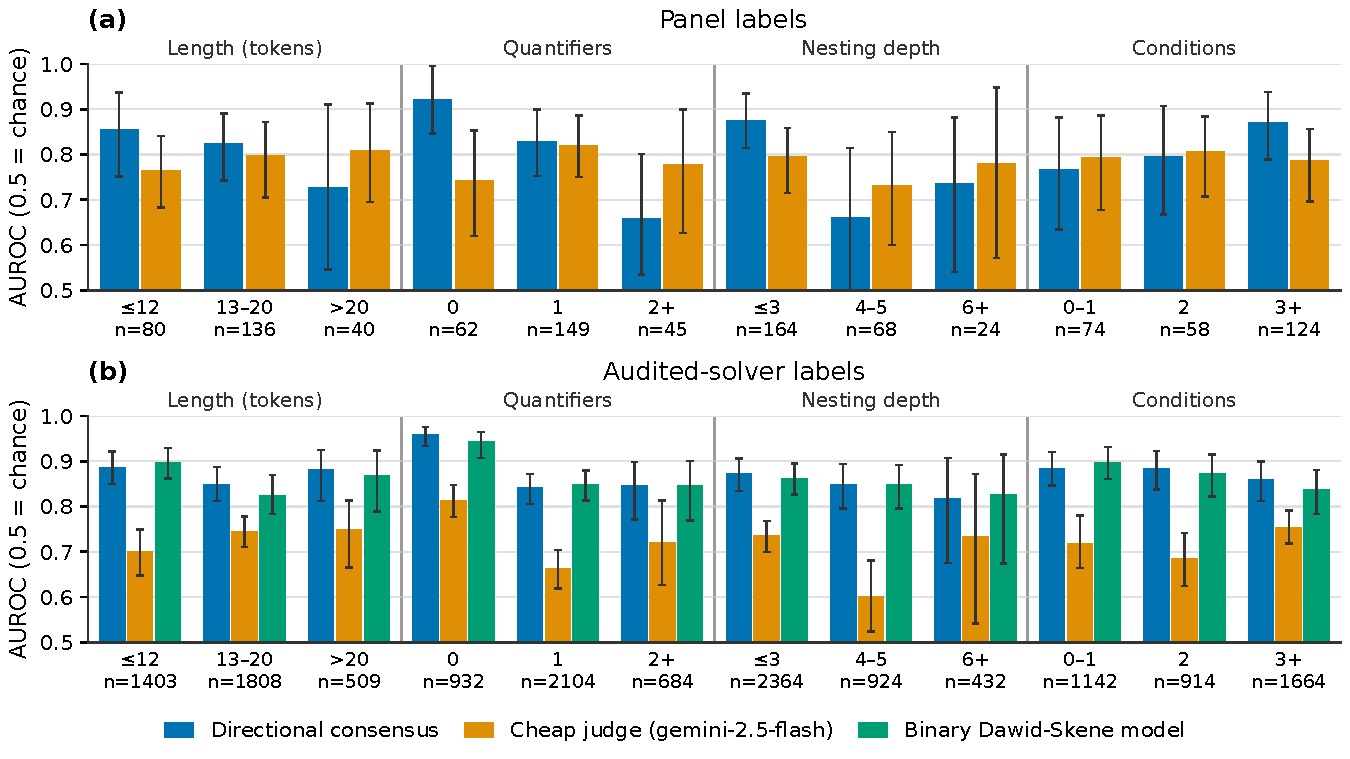
\includegraphics[width=\linewidth,height=0.85\textheight,keepaspectratio]{figures/fig9_v0.pdf}
\caption{Fresh confirmation set: AUROC of directional consensus and the cheap judge in each complexity stratum the user named. (a) Panel labels (n items per stratum in the category labels). (b) Audited-solver labels, with the binary Dawid-Skene model added. Under panel labels agreement leads on short, quantifier-free and shallow items and trails the judge on sentences with two or more quantifiers, nesting depth 4-5 and more than 20 tokens; it also leads on sentences with three or more conditions (0.871 against 0.787). The tercile gap to the judge shrinks (+0.088, +0.107, $-$0.028; slope $-$0.058 [$-$0.135, 0.022], not significant). Solver labels share DC's equivalence checker, so panel (b) is partly circular.}
\label{fig:fig9}
\end{figure}

\subsubsection{Real error types, within a sentence}

Table 49 gives detection per panel error type: AUROC of panel-faithful items against the unfaithful items of one type. Every class has fewer than 30 items, so the table is descriptive. DC and binary Dawid-Skene model are strongest on $\forall$/$\exists$ and implication-direction errors; the cheap judge is strongest on unparseable outputs, negation and quantifier scope. Across 70 faithful $\times$ unfaithful pairs from the same sentence, DC ordered 0.929 [0.864, 0.979] correctly, binary Dawid-Skene model 0.914 [0.857, 0.971], the cheap judge 0.786 [0.714, 0.850], vocabulary conformity 0.736, the local round-trip NLI 0.721 and the local error-typed judge 0.693. The panel sampler built these pairs from one modal and one minority member per sentence, which is the comparison agreement is built for. The development set's shuffle placebo (Table 35) showed that on unselected pairs the within-sentence picture is much weaker.

{\scriptsize
\setlength{\tabcolsep}{3pt}
\begin{longtable}{>{\raggedright\arraybackslash}p{0.103\linewidth}>{\raggedright\arraybackslash}p{0.022\linewidth}>{\raggedright\arraybackslash}p{0.049\linewidth}>{\raggedright\arraybackslash}p{0.133\linewidth}>{\raggedright\arraybackslash}p{0.133\linewidth}>{\raggedright\arraybackslash}p{0.062\linewidth}>{\raggedright\arraybackslash}p{0.121\linewidth}>{\raggedright\arraybackslash}p{0.121\linewidth}>{\raggedright\arraybackslash}p{0.133\linewidth}}
\caption*{\textbf{Table 49.} Fresh panel items: AUROC of faithful items against the unfaithful items of one primary error type (n unfaithful). \textit{[Source: fresh confirmation, \texorpdfstring{\textup{\nolinkurl{gen_art_experiment_3}}}{gen art experiment 3}, iteration 2]}}\\
\toprule
\textbf{Error type} & \textbf{n} & \textbf{DC} & \textbf{DC, unparseable 0} & \textbf{binary Dawid-Skene model} & \textbf{cheap judge} & \textbf{round-trip NLI (L)} & \textbf{vocabulary conformity} & \textbf{error-typed judge (L)} \\
\midrule
\endfirsthead
\multicolumn{9}{l}{\textit{(continued)}}\\
\toprule
\textbf{Error type} & \textbf{n} & \textbf{DC} & \textbf{DC, unparseable 0} & \textbf{binary Dawid-Skene model} & \textbf{cheap judge} & \textbf{round-trip NLI (L)} & \textbf{vocabulary conformity} & \textbf{error-typed judge (L)} \\
\midrule
\endhead
\bottomrule
\endlastfoot
{}added condition & 27 & 0.799 & 0.825 & 0.796 & 0.704 & 0.827 & 0.570 & 0.615 \\
{}$\forall$/$\exists$ choice & 21 & 0.896 & 0.914 & 0.914 & 0.857 & 0.809 & 0.763 & 0.781 \\
{}dropped condition & 14 & 0.785 & 0.800 & 0.817 & 0.747 & 0.860 & 0.788 & 0.503 \\
{}implication direction / ``only'' & 12 & 0.881 & 0.923 & 0.921 & 0.860 & 0.829 & 0.664 & 0.723 \\
{}quantifier scope & 10 & 0.822 & 0.838 & 0.792 & 0.875 & 0.639 & 0.723 & 0.785 \\
{}syntax / unparseable & 7 & 0.732 & 0.770 & 0.736 & 0.963 & 0.731 & 0.521 & 0.890 \\
{}conjunction / disjunction & 6 & 0.810 & 0.863 & 0.751 & 0.704 & 0.809 & 0.545 & 0.567 \\
{}conflation & 6 & 0.843 & 0.840 & 0.812 & 0.714 & 0.716 & 0.883 & 0.550 \\
{}wrong constant & 3 & 0.868 & 0.865 & 0.872 & 0.770 & 0.599 & 0.805 & 0.471 \\
{}negation / polarity & 3 & 0.754 & 0.883 & 0.758 & 0.996 & 0.785 & 0.612 & 0.846 \\
{}other & 3 & 0.763 & 0.760 & 0.753 & 0.654 & 0.603 & 0.485 & 0.471 \\
{}argument swap & 2 & 0.930 & 0.928 & 0.976 & 0.871 & 0.789 & 0.890 & 0.700 \\
{}wrong split & 2 & 0.839 & 0.928 & 0.822 & 0.770 & 0.889 & 0.799 & 0.471 \\
\end{longtable}
}

\subsubsection{Shared bias on fresh data}

The pre-registered boundary appeared on fresh sentences (Table 50). In the 61 panel items from sentences whose modal cluster is wrong, DC falls to 0.419 [0.292, 0.557], below chance, while the cheap judge holds 0.786. Where the mode is right, DC scores 0.883 against the judge's 0.782. Mode correctness is read from the labels, so this split is descriptive.

\begin{table}[H]
\centering
\small
\setlength{\tabcolsep}{3pt}
\caption*{\textbf{Table 50.} AUROC in sentences whose modal cluster is right or wrong. \textit{[Source: fresh confirmation, \texorpdfstring{\textup{\nolinkurl{gen_art_experiment_3}}}{gen art experiment 3}, iteration 2]}}
\begin{tabular}{>{\raggedright\arraybackslash}p{0.339\linewidth}>{\raggedright\arraybackslash}p{0.240\linewidth}>{\raggedright\arraybackslash}p{0.124\linewidth}>{\raggedright\arraybackslash}p{0.236\linewidth}}
\toprule
\textbf{Stratum} & \textbf{DC} & \textbf{cheap judge} & \textbf{majority clustering} \\
\midrule
{}panel, mode right (n = 195) & 0.883 [0.822, 0.934] & 0.782 & 0.867 \\
{}panel, mode wrong (n = 61) & 0.419 [0.292, 0.557] & 0.786 & 0.433 \\
{}solver, mode right (n = 2,167) & 0.912 [0.876, 0.946] & 0.752 & 0.899 \\
{}solver, mode wrong (n = 1,553) & 0.517 [0.458, 0.566] & 0.554 & 0.576 \\
\bottomrule
\end{tabular}
\end{table}

\subsubsection{System level}

Table 51 gives Kendall $\tau$\_\allowbreak{}b between each metric's per-system mean and the per-system faithful rate over the nine systems, with sentence-bootstrap intervals. Under solver labels DC orders the systems best (0.889); under panel labels the cheap judge does (0.833) and DC reaches 0.556. The intervals are wide with nine systems. Per system under solver labels, DC's AUROC ranged from 0.811 (gpt-oss-120b) to 0.902 (llama-3.1-8b) and the cheap judge's from 0.645 (phi-4) to 0.766 (qwen-2.5-7b); DC was above the judge for every system. Table 51b gives the per-system values.

\begin{table}[H]
\centering
\small
\setlength{\tabcolsep}{3pt}
\caption*{\textbf{Table 51.} System-level agreement over 9 systems: Kendall $\tau$\_\allowbreak{}b [95\% CI] and pairwise order accuracy. \textit{[Source: fresh confirmation, \texorpdfstring{\textup{\nolinkurl{gen_art_experiment_3}}}{gen art experiment 3}, iteration 2]}}
\begin{tabular}{>{\raggedright\arraybackslash}p{0.240\linewidth}>{\raggedright\arraybackslash}p{0.173\linewidth}>{\raggedright\arraybackslash}p{0.165\linewidth}>{\raggedright\arraybackslash}p{0.183\linewidth}>{\raggedright\arraybackslash}p{0.165\linewidth}}
\toprule
\textbf{Metric} & \textbf{$\tau$\_\allowbreak{}b panel} & \textbf{pairwise panel} & \textbf{$\tau$\_\allowbreak{}b solver} & \textbf{pairwise solver} \\
\midrule
{}DC & 0.556 [0.222, 0.722] & 0.778 & 0.889 [0.667, 0.944] & 0.944 \\
{}binary Dawid-Skene model & 0.611 [0.222, 0.722] & 0.806 & 0.722 [0.556, 0.889] & 0.861 \\
{}majority clustering & 0.500 [0.111, 0.667] & 0.750 & 0.611 [0.389, 0.778] & 0.806 \\
{}cheap judge & 0.833 [0.389, 0.889] & 0.917 & 0.722 [0.611, 0.889] & 0.861 \\
{}vocabulary conformity & 0.500 [0.167, 0.722] & 0.750 & 0.611 [0.444, 0.778] & 0.806 \\
{}parse rate & 0.479 [0.181, 0.761] & 0.722 & 0.704 [0.479, 0.761] & 0.833 \\
{}structural (user pilot) & 0.500 [0.222, 0.770] & 0.750 & 0.611 [0.457, 0.761] & 0.806 \\
\bottomrule
\end{tabular}
\end{table}

{\small
\setlength{\tabcolsep}{3pt}
\begin{longtable}{>{\raggedright\arraybackslash}p{0.431\linewidth}>{\raggedright\arraybackslash}p{0.106\linewidth}>{\raggedright\arraybackslash}p{0.125\linewidth}>{\raggedright\arraybackslash}p{0.277\linewidth}}
\caption*{\textbf{Table 51b.} Per-system AUROC under solver labels on the fresh set. \textit{[Source: fresh confirmation, \texorpdfstring{\textup{\nolinkurl{gen_art_experiment_3}}}{gen art experiment 3}, iteration 2]}}\\
\toprule
\textbf{System} & \textbf{DC} & \textbf{cheap judge} & \textbf{binary Dawid-Skene model} \\
\midrule
\endfirsthead
\multicolumn{4}{l}{\textit{(continued)}}\\
\toprule
\textbf{System} & \textbf{DC} & \textbf{cheap judge} & \textbf{binary Dawid-Skene model} \\
\midrule
\endhead
\bottomrule
\endlastfoot
{}llama-3.1-8b & 0.902 & 0.719 & 0.900 \\
{}qwen-2.5-7b & 0.902 & 0.766 & 0.895 \\
{}gemma-3-27b & 0.891 & 0.732 & 0.883 \\
{}deepseek-v3.1 & 0.890 & 0.717 & 0.888 \\
{}mistral-small-3.2-24b & 0.882 & 0.733 & 0.861 \\
{}phi-4 & 0.877 & 0.645 & 0.869 \\
{}gemini-2.5-flash & 0.844 & 0.729 & 0.832 \\
{}gpt-4.1-mini & 0.843 & 0.722 & 0.825 \\
{}gpt-oss-120b & 0.811 & 0.677 & 0.802 \\
\end{longtable}
}

\subsubsection{Invariance, contamination and controlled mutants}

Across 1,695 Z3-verified meaning-preserving rewrites of 400 fresh candidates, DC false-alarmed (change above 0.05, a mode flip or a type change) on 0.25\% of synonym renamings and 0.5\% of random renamings, and never on contrapositive, De Morgan or reorder rewrites (Table 52). The renaming flips were changes of the typed error only, never of score or mode, and their count varies by one item between runs because typing searches under a wall-clock limit. The vocabulary-conformity control false-alarmed on 86.4\% of synonym renamings (mean change 0.199). On the development contamination rows, DC's mean change between original and entity-renamed candidates was exactly 0.000 over 936 pairs; those candidates are renamed copies of the originals, not regenerations.

\begin{table}[H]
\centering
\small
\setlength{\tabcolsep}{3pt}
\caption*{\textbf{Table 52.} DC false alarms on solver-verified rewrites of 400 fresh candidates. \textit{[Source: fresh confirmation, \texorpdfstring{\textup{\nolinkurl{gen_art_experiment_3}}}{gen art experiment 3}, iteration 2]}}
\begin{tabular}{>{\raggedright\arraybackslash}p{0.428\linewidth}>{\raggedright\arraybackslash}p{0.214\linewidth}>{\raggedright\arraybackslash}p{0.310\linewidth}}
\toprule
\textbf{Rewrite} & \textbf{n verified} & \textbf{false-alarm rate} \\
\midrule
{}synonym renaming & 396 & 0.0025 \\
{}random renaming & 399 & 0.0050 \\
{}contrapositive & 311 & 0.0000 \\
{}De Morgan & 276 & 0.0000 \\
{}conjunct reorder & 313 & 0.0000 \\
\bottomrule
\end{tabular}
\end{table}

Table 53 gives the controlled mutants, which are mechanism evidence only. Each of 298 greedy candidates proved equivalent to its audited gold (one per sentence) was mutated by one operator, the mutant was kept only if Z3 showed it non-equivalent, and the mutant was scored against the same eight peers. DC detects synthetic errors except argument swaps, which a name-free alignment can absorb by permuting constants. Its typing works for the operators its rules target (added condition 0.72, $\forall$/$\exists$ 0.60) and is near zero for negation and conjunction/disjunction, the first because the literal-flip rule was frozen off and the second because no rule exists. Real panel errors are typed far worse (Table 45).

\begin{table}[H]
\centering
\footnotesize
\setlength{\tabcolsep}{3pt}
\caption*{\textbf{Table 53.} Controlled perturbations of 298 solver-verified faithful anchors. \textit{[Source: fresh confirmation, \texorpdfstring{\textup{\nolinkurl{gen_art_experiment_3}}}{gen art experiment 3}, iteration 2]}}
\begin{tabular}{>{\raggedright\arraybackslash}p{0.153\linewidth}>{\raggedright\arraybackslash}p{0.043\linewidth}>{\raggedright\arraybackslash}p{0.206\linewidth}>{\raggedright\arraybackslash}p{0.133\linewidth}>{\raggedright\arraybackslash}p{0.105\linewidth}>{\raggedright\arraybackslash}p{0.273\linewidth}}
\toprule
\textbf{Operator} & \textbf{n} & \textbf{P(DC(anchor) $>$ DC(mutant)) [95\% CI]} & \textbf{DC typing accuracy} & \textbf{mutant still in mode} & \textbf{vocabulary-conformity detection} \\
\midrule
{}negation & 296 & 0.929 [0.909, 0.949] & 0.020 & 0.051 & 0.500 \\
{}implication reversal & 254 & 0.888 [0.860, 0.915] & 0.228 & 0.130 & 0.500 \\
{}added conjunct & 254 & 0.913 [0.886, 0.939] & 0.720 & 0.079 & 0.960 \\
{}$\wedge$ $\leftrightarrow$ $\vee$ & 204 & 0.919 [0.895, 0.944] & 0.000 & 0.064 & 0.500 \\
{}$\forall$ $\leftrightarrow$ $\exists$ & 207 & 0.872 [0.838, 0.908] & 0.599 & 0.082 & 0.500 \\
{}dropped conjunct & 163 & 0.887 [0.850, 0.920] & 0.497 & 0.086 & 0.923 \\
{}argument swap & 51 & 0.647 [0.559, 0.735] & 0.196 & 0.157 & 0.500 \\
\bottomrule
\end{tabular}
\end{table}

\subsubsection{Wrong gold, coverage, cost and what was not run}

With the shipped gold as a tenth peer, 1 $-$ DC of the gold predicted the gold audit's ``wrong'' verdict at AUROC 0.859 on the 450 fresh golds (base rate 0.458), with precision@50 of 0.80. Over 14,520 fresh greedy pairs, the relations were EQUIV 38.5\%, INCOMPARABLE 31.5\%, WEAKER 11.3\%, STRONGER 9.6\%, UNALIGNABLE 9.0\% and CONTRADICTORY 0.1\%; timeouts were 0.14\%, all in pairs of 13 to 20 atoms, and equivalence was never non-transitive. Of the covered DC scores, 32.3\% were exactly 0 and 11.2\% exactly 1. DC costs no API call when peers exist and 0.158 s of solver time per item (p95 0.528 s); if the eight peers must be generated for scoring it costs \$0.00039 per item, against \$0.000030 for the cheap judge. The artifact spent \$2.38 (gold audit \$0.876, panel adjudication \$0.806, generation \$0.454, calibration \$0.150, cheap judge \$0.099).

On the development anchor only, a stack of [cheap judge, parse, DC] reached out-of-fold 0.796 against gemini-2.5-pro's 0.825 on the 609 panel items; the frontier judge was not run on fresh items. The arbiter, the frontier judge, the EU-AI-Act transfer and the rule-marker signature as a secondary stack feature were not run. The session also received only the last 200 characters of its task prompt, and the prompt was reconstructed from the sibling sessions' identical template; the plan was followed as written.

\subsection{Directional consensus on long legal definitions (\texorpdfstring{\textup{\nolinkurl{gen_art_experiment_5}}}{gen art experiment 5})}

This subsection reports the artifact \texorpdfstring{\textup{\nolinkurl{gen_art_experiment_5}}}{gen art experiment 5}.

\subsubsection{What was built}

This artifact is the run's first labelled test on exception-heavy text. It built 158 legal sentences: the 68 definitions of Article 3 of the EU AI Act from the user's pilot upload, 59 public statutory items (GDPR Art. 4, DSA Art. 3, DMA Art. 2 and Data Act Art. 2 from EUR-Lex, and 19 clauses from the SARA US tax-code set), and 31 other AI-Act sentences used as a pre-declared top-up where a marker bin ran out. Each sentence was binned by the number of ten exception and condition markers it contains (``unless'', ``except'', ``other than'', ``provided that'', ``only'', ``where'', ``not'', ``excluding'', ``including'', ``without prejudice''): we call sentences with at most one marker \emph{low-marker}, with two or three \emph{mid-marker}, and with four or more \emph{high-marker}. The three bins hold 91, 51 and 16 sentences, with mean lengths of 35, 63 and 100 tokens; sentences with four or more markers are rare in statutory text in every source. The nine systems translated each sentence with the frozen prompt (max\_\allowbreak{}tokens raised to 1,024, truncating 0.6\% of outputs), giving a greedy parse rate of 73.3\%. The user's 367 pilot formulas form a tenth family.

DC here is the contract's third implementation, with all three alignment levels but granularity definitions restricted before any label to conjunctions of two positive literals, because the toy tests showed negated definitions absorbing a dropped exception (Bird := Bird $\wedge$ $\neg$Penguin). It was frozen before the first panel label was read. On the 609 development panel items this implementation scored 0.774 [0.721, 0.824]; the other two scored 0.769 (Section 6.2) and 0.777 (Section 6.3) on the same items, so the three implementations agree on the anchor within 0.008. On 500 development pairs its relations agreed exactly with the confirmation artifact's on 80\% and on equivalence-versus-not on 97\%; on 300 legal pairs the figures were 67\% and 99\%.

The labels come from the same calibrated three-member panel (claude-haiku-4.5 0.875, grok-4.3 0.950, glm-4.6 0.850 on the gate), judging each candidate from the sentence alone, since no gold exists. A sample of 480 system items and 200 pilot items was drawn with a seed before any label existed, and 655 were labelled before the budget stop (645 with three votes, 10 with two). Only 67 are faithful, a weighted 9.4\%. Table 54 gives the panel's agreement, which is lower than on public corpora and falls with marker count.

\begin{table}[H]
\centering
\small
\setlength{\tabcolsep}{3pt}
\caption*{\textbf{Table 54.} Panel labels on the legal set. \textit{[Source: legal-text transfer test, \texorpdfstring{\textup{\nolinkurl{gen_art_experiment_5}}}{gen art experiment 5}, iteration 2]}}
\begin{tabular}{>{\raggedright\arraybackslash}p{0.450\linewidth}>{\raggedright\arraybackslash}p{0.514\linewidth}}
\toprule
\textbf{Quantity} & \textbf{Value} \\
\midrule
{}labelled items (faithful / unfaithful) & 655 (67 / 588) \\
{}weighted faithful share; Kish effective positives / negatives & 0.094; 60.7 / 521.7 \\
{}unanimous share & 0.798 \\
{}Fleiss $\kappa$ overall (645 items) / low / mid / high marker bin & 0.382 / 0.417 / 0.218 / 0.170 \\
{}pairwise Cohen $\kappa$ haiku-grok / haiku-glm / grok-glm & 0.497 / 0.447 / 0.255 \\
{}member faithful rate haiku / grok / glm & 0.109 / 0.223 / 0.040 \\
{}weighted faithful share by marker bin, low / mid / high & 0.123 / 0.033 / 0.069 \\
{}weighted faithful share by system & gemini-2.5-flash 0.194, gpt-4.1-mini 0.184, gpt-oss-120b 0.144, qwen-2.5-7b 0.100, phi-4 0.096, mistral-small 0.071, gemma-3-27b 0.064, pilot 0.063, deepseek-v3.1 0.054, llama-3.1-8b 0.006 \\
\bottomrule
\end{tabular}
\end{table}

\subsubsection{Results}

Table 55 gives every metric against the panel labels. DC scores 0.705 and passes its pre-registered floor (point $\geq$ 0.70, one-sided lower bound 0.62 $>$ 0.5). The cheap judge dominates everything at 0.927, above gemini-2.5-pro at 0.852. Majority clustering (0.754) is above DC, and part of that gap is the contract's 0.5 score for unparseable candidates, which majority clustering scores 0: on parseable items DC is 0.796 against 0.786, and a post-hoc DC that scores unparseable candidates 0 reaches 0.764. A placebo that gives each candidate peers from another sentence scores 0.506.

{\small
\setlength{\tabcolsep}{3pt}
\begin{longtable}{>{\raggedright\arraybackslash}p{0.536\linewidth}>{\raggedright\arraybackslash}p{0.184\linewidth}>{\raggedright\arraybackslash}p{0.060\linewidth}>{\raggedright\arraybackslash}p{0.159\linewidth}}
\caption*{\textbf{Table 55.} Weighted AUROC against panel labels on the legal set (655 items unless stated). Round-trip scores use local Qwen3-8B back-translation. \textit{[Source: legal-text transfer test, \texorpdfstring{\textup{\nolinkurl{gen_art_experiment_5}}}{gen art experiment 5}, iteration 2]}}\\
\toprule
\textbf{Metric} & \textbf{AUROC [95\% CI]} & \textbf{n} & \textbf{coverage} \\
\midrule
\endfirsthead
\multicolumn{4}{l}{\textit{(continued)}}\\
\toprule
\textbf{Metric} & \textbf{AUROC [95\% CI]} & \textbf{n} & \textbf{coverage} \\
\midrule
\endhead
\bottomrule
\endlastfoot
{}DC (frozen) & 0.705 [0.608, 0.792] & 655 & 0.750 \\
{}DC, structural-fingerprint map order & 0.712 [0.615, 0.799] & 655 & 0.750 \\
{}DC without granularity definitions & 0.672 [0.574, 0.763] & 655 & 0.747 \\
{}DC, unweighted & 0.656 [0.572, 0.739] & 655 & 0.750 \\
{}Dawid-Skene model over DC clusters & 0.760 [0.652, 0.859] & 492 & 0.766 \\
{}majority clustering & 0.754 [0.670, 0.828] & 655 & 0.760 \\
{}binary Dawid-Skene model & 0.729 [0.630, 0.824] & 464 & 0.752 \\
{}DC + arbiter (local judge) & 0.610 [0.530, 0.690] & 655 & 1.000 \\
{}DC with own samples as peers & 0.742 [0.615, 0.866] & 315 & 0.733 \\
{}sampling self-consistency & 0.821 [0.676, 0.942] & 124 & 0.782 \\
{}predicate-set Jaccard across samples (user pilot metric) & 0.755 [0.606, 0.885] & 124 & 1.000 \\
{}cheap judge (gemini-2.5-flash) & 0.927 [0.900, 0.949] & 655 & 1.000 \\
{}frontier judge (gemini-2.5-pro) & 0.852 [0.786, 0.904] & 655 & 1.000 \\
{}round-trip NLI (L) & 0.694 [0.601, 0.773] & 655 & 1.000 \\
{}round-trip cosine (L) & 0.691 [0.620, 0.762] & 655 & 1.000 \\
{}vocabulary conformity & 0.685 [0.599, 0.766] & 655 & 0.760 \\
{}structural (user pilot) & 0.597 [0.540, 0.650] & 655 & 1.000 \\
{}structural: arity within formula / within act / joint load & 0.572 / 0.596 / 0.569 & 655 & 1.000 \\
{}parse rate & 0.569 [0.515, 0.615] & 655 & 1.000 \\
{}placebo, peers from another sentence & 0.506 [0.460, 0.554] & 498 & 0.938 \\
\end{longtable}
}

The artifact's \texttt{results/\allowbreak{}tests.json} also splits the labelled items into the nine systems' outputs (frame A, excluding the user's pilot formulas) and the pilot formulas (frame B), and reports the covered-only frame. The run's report text gave frame B in prose and omitted frame A, which the iteration-2 review asked for; Table 55a gives all three from the file. The cheap judge leads in every frame; on the system outputs alone DC is 0.024 higher than on the pooled set and still 0.202 below the judge.

{\small
\setlength{\tabcolsep}{3pt}
\begin{longtable}{>{\raggedright\arraybackslash}p{0.221\linewidth}>{\raggedright\arraybackslash}p{0.239\linewidth}>{\raggedright\arraybackslash}p{0.244\linewidth}>{\raggedright\arraybackslash}p{0.235\linewidth}}
\caption*{\textbf{Table 55a.} Legal-set AUROC by frame (added for this record from \texttt{results/\allowbreak{}tests.json}, block X1; weighted, 95\% CIs). \textit{[Source: legal-text transfer test, \texorpdfstring{\textup{\nolinkurl{gen_art_experiment_5}}}{gen art experiment 5}, iteration 2]}}\\
\toprule
\textbf{Metric} & \textbf{A: system outputs only (464 items, 55 faithful, 153 sentences)} & \textbf{B: user pilot formulas only (191 items, 12 faithful, 63 sentences)} & \textbf{covered items only (491 items, 60 faithful, 141 sentences)} \\
\midrule
\endfirsthead
\multicolumn{4}{l}{\textit{(continued)}}\\
\toprule
\textbf{Metric} & \textbf{A: system outputs only (464 items, 55 faithful, 153 sentences)} & \textbf{B: user pilot formulas only (191 items, 12 faithful, 63 sentences)} & \textbf{covered items only (491 items, 60 faithful, 141 sentences)} \\
\midrule
\endhead
\bottomrule
\endlastfoot
{}DC & 0.729 [0.634, 0.818] & 0.537 [0.340, 0.793] & 0.802 [0.715, 0.883] \\
{}DC without granularity definitions & 0.690 [0.598, 0.780] & 0.537 [0.340, 0.793] & n/a \\
{}DC with own samples as peers & 0.828 [0.672, 0.960] (n = 124) & 0.633 [0.376, 0.845] & n/a \\
{}majority clustering & 0.772 [0.689, 0.853] & 0.629 [0.500, 0.833] & 0.786 [0.698, 0.869] \\
{}binary Dawid-Skene model & 0.729 [0.630, 0.824] & n/a & n/a \\
{}vocabulary conformity & 0.703 [0.623, 0.778] & 0.581 [0.305, 0.837] & 0.800 [0.702, 0.882] \\
{}round-trip NLI (L) & 0.679 [0.579, 0.767] & 0.767 [0.491, 0.906] & n/a \\
{}parse rate & 0.563 [0.503, 0.616] & 0.615 [0.573, 0.661] & n/a \\
{}cheap judge & 0.931 [0.906, 0.954] & 0.899 [0.780, 0.978] & 0.918 [0.887, 0.943] \\
{}frontier judge & 0.876 [0.817, 0.925] & 0.684 [0.412, 0.855] & 0.835 [0.757, 0.896] \\
\end{longtable}
}

The increment test passed marginally over [cheap judge, parse] (Table 56): +0.021 with a one-sided bound of +0.002, and +0.034 [0.007, 0.067] on covered items only. Over the full base with round-trip and structural features it gave +0.008 [$-$0.012, 0.028], no increment. The frontier judge is 0.075 below the cheap judge against these labels.

{\small
\setlength{\tabcolsep}{3pt}
\begin{longtable}{>{\raggedright\arraybackslash}p{0.671\linewidth}>{\raggedright\arraybackslash}p{0.293\linewidth}}
\caption*{\textbf{Table 56.} Stacking contrasts on the legal set (cross-fitted, 655 items). \textit{[Source: legal-text transfer test, \texorpdfstring{\textup{\nolinkurl{gen_art_experiment_5}}}{gen art experiment 5}, iteration 2]}}\\
\toprule
\textbf{Contrast} & \textbf{$\Delta$ [95\% CI]} \\
\midrule
\endfirsthead
\multicolumn{2}{l}{\textit{(continued)}}\\
\toprule
\textbf{Contrast} & \textbf{$\Delta$ [95\% CI]} \\
\midrule
\endhead
\bottomrule
\endlastfoot
{}[cheap judge, parse, DC] $-$ [cheap judge, parse] (base 0.906 $\rightarrow$ 0.927) & +0.021 [$-$0.001, 0.046] \\
{}same, covered items only (n = 491) & +0.034 [0.007, 0.067] \\
{}random-feature placebo & +0.003 [$-$0.005, 0.012] \\
{}full base [judge, parse, round-trip NLI, round-trip cosine, structural] + DC & +0.008 [$-$0.012, 0.028] \\
{}DC $-$ majority clustering & $-$0.049 [$-$0.113, 0.016] \\
{}DC $-$ binary Dawid-Skene model (n = 464) & $-$0.000 [$-$0.111, 0.110] \\
{}DC $-$ vocabulary conformity & +0.019 [$-$0.032, 0.066] \\
{}DC $-$ DC without granularity definitions & +0.033 [$-$0.003, 0.087] \\
{}[judge, parse, DC] $-$ frontier judge & +0.075 [0.028, 0.133] \\
{}frontier judge $-$ cheap judge & $-$0.075 [$-$0.134, $-$0.026] \\
{}[judge, parse, frontier judge] + DC & +0.022 [0.001, 0.048] \\
\end{longtable}
}

The complexity question has its first labelled answer on legal text, and it is negative for DC (Table 57). DC trails the cheap judge in every marker bin. The mid-marker and high-marker bins have 6 and 5 faithful items, so they are underpowered, and the within-sentence slope of the gap on marker count is $-$0.046 [$-$0.133, 0.113], inconclusive rather than positive. Coverage falls with markers, mostly through parse failures.

\begin{table}[H]
\centering
\scriptsize
\setlength{\tabcolsep}{3pt}
\caption*{\textbf{Table 57.} Legal set by marker bin (weighted AUROC; n items, n faithful). \textit{[Source: legal-text transfer test, \texorpdfstring{\textup{\nolinkurl{gen_art_experiment_5}}}{gen art experiment 5}, iteration 2]}}
\begin{tabular}{>{\raggedright\arraybackslash}p{0.114\linewidth}>{\raggedright\arraybackslash}p{0.050\linewidth}>{\raggedright\arraybackslash}p{0.064\linewidth}>{\raggedright\arraybackslash}p{0.100\linewidth}>{\raggedright\arraybackslash}p{0.123\linewidth}>{\raggedright\arraybackslash}p{0.123\linewidth}>{\raggedright\arraybackslash}p{0.123\linewidth}>{\raggedright\arraybackslash}p{0.077\linewidth}>{\raggedright\arraybackslash}p{0.100\linewidth}}
\toprule
\textbf{Bin (n, faithful)} & \textbf{DC} & \textbf{cheap judge} & \textbf{frontier judge} & \textbf{round-trip NLI (L)} & \textbf{vocabulary conformity} & \textbf{majority clustering} & \textbf{DC $-$ judge [95\% CI]} & \textbf{DC coverage} \\
\midrule
{}low-marker, 0-1 (419, 56) & 0.726 & 0.923 & 0.862 & 0.728 & 0.693 & 0.795 & $-$0.197 [$-$0.299, $-$0.108] & 0.79 \\
{}mid-marker, 2-3 (162, 6) & 0.566 & 0.931 & 0.823 & 0.534 & 0.575 & 0.548 & $-$0.365 [$-$0.583, $-$0.084] & 0.74 \\
{}high-marker, $\geq$ 4 (74, 5) & 0.685 & 0.909 & 0.785 & 0.685 & 0.718 & 0.493 & $-$0.224 [$-$0.655, $-$0.105] & 0.54 \\
\bottomrule
\end{tabular}
\end{table}

Within a sentence (Table 58), DC ordered exception-involved errors correctly 0.878 of the time against the cheap judge's 0.716 over 37 pairs, with wide intervals, and trailed the judge on dropped and added conditions. Its error naming failed: weighted top-1 0.044 against 0.219 for always answering ``dropped condition'', with 86\% of items typed ``other''.

\begin{table}[H]
\centering
\footnotesize
\setlength{\tabcolsep}{3pt}
\caption*{\textbf{Table 58.} Within-sentence ordering on the legal set, P(faithful partner scores above the error), by the panel's primary error type. \textit{[Source: legal-text transfer test, \texorpdfstring{\textup{\nolinkurl{gen_art_experiment_5}}}{gen art experiment 5}, iteration 2]}}
\begin{tabular}{>{\raggedright\arraybackslash}p{0.242\linewidth}>{\raggedright\arraybackslash}p{0.102\linewidth}>{\raggedright\arraybackslash}p{0.102\linewidth}>{\raggedright\arraybackslash}p{0.129\linewidth}>{\raggedright\arraybackslash}p{0.177\linewidth}>{\raggedright\arraybackslash}p{0.161\linewidth}}
\toprule
\textbf{Error type (pairs)} & \textbf{DC} & \textbf{cheap judge} & \textbf{frontier judge} & \textbf{DC without granularity} & \textbf{majority clustering} \\
\midrule
{}dropped condition (20) & 0.625 [0.40, 0.81] & 0.875 [0.727, 0.979] & 0.650 & 0.650 & 0.600 \\
{}added condition (44) & 0.682 [0.474, 0.848] & 0.886 [0.793, 0.964] & 0.773 & 0.716 & 0.761 \\
{}implication direction / ``only'' (83) & 0.837 [0.679, 0.932] & 0.837 [0.687, 0.980] & 0.837 & 0.831 & 0.843 \\
{}exception-involved (37) & 0.878 [0.5, 1.0] & 0.716 [0.6, 1.0] & 0.986 & 0.878 & 0.919 \\
{}any unfaithful (210) & 0.717 [0.595, 0.826] & 0.843 [0.763, 0.916] & 0.740 & 0.717 & 0.738 \\
\bottomrule
\end{tabular}
\end{table}

On the two sampled systems, DC with a system's own samples as peers scored 0.828 against sampling self-consistency's 0.821 ($\Delta$ +0.006 [$-$0.041, 0.075]; n = 124). On the pilot formulas it scored 0.633 against 0.436 for the user's cross-run Jaccard metric and 0.540 for the user's consistency metric; the cheap judge scored 0.899 there, and DC with the nine systems as peers scored 0.537 [0.340, 0.793] (191 pilot items, 12 faithful).

The shared-bias boundary is stronger on legal text than anywhere else. In 76\% of the 62 sentences with a labelled mode, the modal cluster is panel-unfaithful. Where the mode is faithful (15 sentences, 90 items), DC reaches 0.889 and the judge 0.885; where it is unfaithful (47 sentences, 241 items, 8 faithful), DC falls to 0.624 [0.370, 0.817] and the judge holds 0.946. Equivalence is rare on long text: only 4.8\% of legal pairs were EQUIV (6.1\%, 1.4\% and 1.6\% in the low-, mid- and high-marker bins), against 38.5\% of pairs on the fresh short sentences in the confirmation artifact's cache; the artifact's own count of equivalence agreement is 6\% on legal pairs against 19\% on its development anchor. As a result every system's one-coin model sensitivity fell below 0.5 and every Dawid-Skene model weight sat at the 0.05 floor. DC on legal text is effectively unweighted.

The panel labels themselves are the weakest point of this test (Table 59). DC ranges from 0.587 to 0.814 depending on which single member provides the label, and reaches 0.866 on the 515 unanimous items, where the cheap judge reaches 0.974. The cheap judge ranks first under every labelling. The planned check of whether the panel can see exception errors in long formulas (30 mutants $\times$ 3 members) was not run, so the panel's sensitivity to exceptions is uncertified.

\begin{table}[H]
\centering
\footnotesize
\setlength{\tabcolsep}{3pt}
\caption*{\textbf{Table 59.} Label robustness: AUROC under each single member's labels and on unanimous items only, with the increment over [cheap judge, parse]. \textit{[Source: legal-text transfer test, \texorpdfstring{\textup{\nolinkurl{gen_art_experiment_5}}}{gen art experiment 5}, iteration 2]}}
\begin{tabular}{>{\raggedright\arraybackslash}p{0.218\linewidth}>{\raggedright\arraybackslash}p{0.076\linewidth}>{\raggedright\arraybackslash}p{0.093\linewidth}>{\raggedright\arraybackslash}p{0.144\linewidth}>{\raggedright\arraybackslash}p{0.179\linewidth}>{\raggedright\arraybackslash}p{0.203\linewidth}}
\toprule
\textbf{Labels (n, weighted faithful)} & \textbf{DC} & \textbf{cheap judge} & \textbf{frontier judge} & \textbf{majority clustering} & \textbf{DC increment [95\% CI]} \\
\midrule
{}haiku only (650, 0.101) & 0.690 & 0.933 & 0.845 & 0.738 & +0.022 [0.003, 0.044] \\
{}grok only (654, 0.208) & 0.587 & 0.843 & 0.827 & 0.638 & +0.005 [$-$0.007, 0.018] \\
{}glm only (651, 0.035) & 0.814 & 0.941 & 0.888 & 0.841 & +0.043 [0.001, 0.096] \\
{}unanimous only (515, 0.040) & 0.866 & 0.974 & 0.932 & 0.886 & +0.032 [0.002, 0.068] \\
\bottomrule
\end{tabular}
\end{table}

The error mix on legal text differs from the public corpora's (Table 60; total variation distance 0.35 [0.32, 0.39]). Dropped conditions lead, and implication direction triples, mostly definitions of the form ``X means Y'' written with $\rightarrow$ instead of $\leftrightarrow$. 24\% of unfaithful items involve an exception.

{\small
\setlength{\tabcolsep}{3pt}
\begin{longtable}{>{\raggedright\arraybackslash}p{0.574\linewidth}>{\raggedright\arraybackslash}p{0.159\linewidth}>{\raggedright\arraybackslash}p{0.218\linewidth}}
\caption*{\textbf{Table 60.} Primary error types among panel-unfaithful legal items (weighted), against the public-corpus mix of Table 23. \textit{[Source: legal-text transfer test, \texorpdfstring{\textup{\nolinkurl{gen_art_experiment_5}}}{gen art experiment 5}, iteration 2]}}\\
\toprule
\textbf{Error type} & \textbf{legal} & \textbf{public (Table 23)} \\
\midrule
\endfirsthead
\multicolumn{3}{l}{\textit{(continued)}}\\
\toprule
\textbf{Error type} & \textbf{legal} & \textbf{public (Table 23)} \\
\midrule
\endhead
\bottomrule
\endlastfoot
{}dropped condition & 0.205 & 0.144 \\
{}implication direction / ``only'' & 0.176 & 0.084 \\
{}added condition & 0.148 & 0.249 \\
{}conjunction / disjunction & 0.102 & 0.041 \\
{}syntax / unparseable & 0.089 & 0.058 \\
{}conflation & 0.069 & 0.043 \\
{}quantifier scope & 0.045 & 0.056 \\
{}argument swap & 0.042 & 0.015 \\
{}exception misplaced & 0.033 & n/a \\
{}$\forall$/$\exists$ choice & 0.032 & 0.218 \\
{}negation / polarity & 0.024 & 0.032 \\
{}other & 0.018 & n/a \\
{}wrong constant & 0.006 & 0.039 \\
{}wrong split & 0.006 & 0.008 \\
{}cardinality / numeric & 0.004 & 0.014 \\
\end{longtable}
}

The remaining checks were descriptive. Over nine systems, Kendall $\tau$\_\allowbreak{}b of per-system mean DC against the panel faithful rate was $-$0.167 (pairwise accuracy 0.417), against 0.556 for the cheap judge and 0.366 for parse rate. Invariance false alarms were 0\% for renaming (100 candidates), 1\% for reorder and 2.0\% for contrapositive (49). The 21 sentences with cross-references scored 0.694 (coverage 0.46) against 0.708 for the rest. DC needed 1.3 CPU-s per scored item and no API call when peers exist, or \$0.0019 per item if the peers must be generated for long text; the cheap judge cost \$0.000062, the frontier judge \$0.0011 and the panel \$0.0051 per item. The artifact spent \$4.65, of which \$3.35 went to the panel and \$0.74 to the frontier judge. Unit tests passed 16 of 20; the four failures are documented identifiability limits (positive granularity against a dropped conjunct, CONTRADICTORY outranked by partial maps, one implication swap typed ``other''). Contamination was not tested, and the pilot's grounded and ungrounded conditions were pooled and never analysed, since that comparison is out of scope.

\subsection{Checks run for this report}

\texttt{checks/\allowbreak{}verify\_\allowbreak{}\allowbreak{}iter2.py} recomputes, from the artifacts' own per-item rows, the panel and solver AUROCs of the fresh confirmation, the legal-set AUROCs, and the development stress test's verdict counts. The fresh panel AUROCs matched Table 44 to three decimals, as reported in Section 6.3. On the legal set the recomputation gave DC 0.705, cheap judge 0.927, frontier judge 0.852, majority clustering 0.754, vocabulary conformity 0.685 and parse rate 0.569, matching Table 55. The verdict recount gave 9 pass, 10 fail and 1 not run.

The three DC implementations are not interchangeable in detail. They share a development anchor within 0.008 AUROC and agree on equivalence-versus-not for 97\% of development pairs, but they chose different defaults for granularity definitions: kept in full in Section 6.2, dropped in Section 6.3, restricted to positive literals in Section 6.4. The confirmation's configuration is the one the pre-registered tests used.

\subsection{What iteration 2 established}

\textbf{Directional consensus on fresh sentences.} On 450 new sentences from nine systems, DC scored 0.827 under panel labels and 0.874 under audited-solver labels, and it added to the frozen judge-plus-round-trip-plus-structural base under both labels (+0.033, lower bound +0.005; +0.118). This is the first time in the run that a gold-free candidate passed an increment test on sentences it had never seen, under labels that do not share its machinery. It did not beat agreement scored by the binary Dawid-Skene model on panel labels (0.827 against 0.830), and the ladder attributes its gain to the reliability weights, not to direction, partial maps or granularity. What passed is cross-output agreement, of the kind round 2 already had; the directional parts of the hypothesis did not add signal. It is also not new in kind: agreement among equivalence-clustered outputs is the mechanism of [33] and [31], and DC's step beyond majority clustering (+0.030 on panel labels, +0.015 solver) came from the weights.

\begin{correction}\textbf{Correction (review of iteration 2).} ``The first time in the run that a gold-free candidate passed an increment test'' depends on the switch from round 2's two-sided 95\% bound to the one-sided bound of Table 27. Under round 2's rule the fresh panel increment fails; under the one-sided rule round 2's majority agreement roughly passes. The fair reading is a consistent +0.02 to +0.03 increment in both populations, significant only under the one-sided rule (Section 6.8).\end{correction}

\textbf{Where agreement stops.} Its pre-registered boundary is real and severe. When the majority is wrong, DC falls below chance on fresh sentences (0.419) and to 0.624 on legal definitions, while the cheap judge keeps 0.786 and 0.946; under constructed shared error the curve is exactly the arithmetic of peer mass. On long legal definitions, where 76\% of modal clusters are unfaithful and only 4.8\% of pairs are equivalent, DC (0.705) is far below the cheap judge (0.927) in every marker bin. Most of DC's item-level AUROC on the development set separated sentences rather than candidates (shuffle placebo 0.73).

\textbf{What DC does that no other metric here does.} It is exactly name-blind: renaming never moved its score at $\delta$ = 0.10 across 999 development candidates and 795 fresh renamings, the cheap judge loses 0.151 AUROC when formulas are written in random tokens, and DC's contamination shift was 0.002 against the judge's 0.096. As a wrong-gold flag with the gold as a tenth peer it reached 0.837 on development golds and 0.859 on fresh golds, and it adds 0.048 to 0.070 to a judge run on the gold.

\textbf{Dead ends recorded in this iteration.}

\begin{itemize}
\item {}Directional error typing. Weighted top-1 0.122 on fresh panel items (majority class 0.255), 0.213 on development items (majority 0.257), 0.044 on legal items (majority 0.219). The net strength profile ranks candidates below chance (0.415). The mechanism prediction that direction would lift added conditions failed on the ladder.
\item {}Granularity definitions (level 3). They absorb negations (constructed detection 0.511 against 1.000 without them) and dropped restrictors (0.659 against 0.995), add 11.9\% spurious equivalence between unrelated sentences, and lower AUROC on the fresh ladder.
\item {}DC as a lone-output metric. With a system's own samples as peers it equals sampling self-consistency to three decimals on fresh data (0.842 against 0.843) and within 0.006 on legal data.
\item {}The complexity prediction for agreement. DC's lead over the cheap judge shrinks with quantifiers, nesting and length on fresh sentences, and DC trails the judge in every legal marker bin.
\item {}The text-anchored arbiter as a repair for shared bias. Not run on gemini; its local Qwen3-8B substitute lowered DC on legal text from 0.705 to 0.610.
\end{itemize}
\textbf{What was not run, and why.} The frontier judge on fresh items, the arbiter on gemini, the long-text exception-sensitivity check of the panel, the EU-AI-Act items inside the confirmation artifact and the rule-marker signature as a secondary stack feature were all cut when the shared \$7.00 key ran out. Spend this iteration was \$2.38 + \$0.088 + \$4.65 = \$7.12, the whole phase budget.

\subsection{What the next iteration takes from it}

This was the last iteration the run allows, so what follows is the open question the record hands on rather than a plan. Cross-output agreement is now a confirmed complement to a cheap judge on short public-benchmark sentences under two label families, and it fails exactly where the user most needs a metric: long, exception-heavy definitions where most systems share the same mistake. The open question is whether any gold-free, text-blind signal can detect shared-bias mistranslation, or whether that regime needs a metric that reads the text. The run's evidence points to the second. On legal text the only metrics that held up were text-reading judges, and the one text-anchored repair that was tried ran on a local substitute. Three measurements would settle it: the arbiter on the saved 1,402 prompts with the frozen gemini judge (about \$0.10), the panel's exception-sensitivity check, and a human-adjudicated sample of legal items, since panel $\kappa$ on four-marker sentences was 0.17.

\begin{correction}\textbf{Correction (review of iteration 2).} The legal-text reading above rests on labels that are themselves sentence-only LLM-panel judgments (Fleiss $\kappa$ 0.17 to 0.42 by marker bin, exception sensitivity uncertified). The same caveat the report applied to the frontier judge in round 2 applies here: LLM judges may agree with an LLM panel. The cheap judge scoring 0.075 above gemini-2.5-pro on these labels is unexplained. ``Confirmed complement'' also overstates the pre-registered outcome, which was ``not supported as stated'' (Section 6.3).\end{correction}

\subsection{The review of the iteration-2 record, and the hypothesis update}

The reviewer scored the report after iteration 2 at 5 of 10, not blocking, with results reported and coverage partial (Table 61a). The reviewer recomputed the headline numbers from the artifacts' per-item files and found them reproducing: the fresh panel AUROCs to four decimals (DC 0.8267, unparseable-as-0 0.8534, binary Dawid-Skene 0.8295, one-coin 0.8338, majority 0.7969, cheap judge 0.7913, vocabulary conformity 0.6744), the solver AUROCs exactly when labels come from the audited solver status (DC 0.874, judge 0.727), the legal AUROCs, the development anchor, the wrong-gold flag, the verdict counts and the Table 37 re-scoring. The objections concerned inference and proportionality, not bookkeeping.

{\small
\setlength{\tabcolsep}{3pt}
\begin{longtable}{>{\raggedright\arraybackslash}p{0.281\linewidth}>{\raggedright\arraybackslash}p{0.684\linewidth}}
\caption*{\textbf{Table 61a.} The review of the iteration-2 record: scores and objections, from the run's iteration records. \textit{[Source: review of the iteration-2 record and hypothesis update (iteration records, iteration 2)]}}\\
\toprule
\textbf{Item} & \textbf{Content} \\
\midrule
\endfirsthead
\multicolumn{2}{l}{\textit{(continued)}}\\
\toprule
\textbf{Item} & \textbf{Content} \\
\midrule
\endhead
\bottomrule
\endlastfoot
{}overall score & 5 of 10, not blocking; results reported: yes; coverage: partial \\
{}soundness & 2: the tables reproduce, but the ``first pass'' rests on a changed criterion, the legal conclusion on LLM-panel labels without the caveat applied elsewhere, and a placebo is misapplied to the signature's within-sentence lead \\
{}presentation & 3: dense but navigable; family headings (``confirmed'', ``closed, negative'') stronger than the pre-registered outcomes beneath them \\
{}contribution & 3: nearly everything preserved; the vocabulary-conformity quintile table and the legal frame A were missing, and one untested lead was missing from the open list \\
{}major: rigor & the T1 ``first pass'' comes from switching a two-sided 95\% bound (round 2) to a one-sided bound (Table 27); by the reviewer's normal approximation, majority agreement's round-2 +0.028 [$-$0.002, 0.056] gives a one-sided bound near +0.003, the one-coin model near 0.000 and even the rule-marker signature near +0.001 \\
{}major: rigor & the legal conclusion rests on sentence-only LLM-panel labels ($\kappa$ 0.38 overall, 0.17 on high-marker sentences); the cheap judge beating the frontier judge by 0.075 suggests judge-to-judge agreement \\
{}major: evidence & the signature's within-sentence lead was discounted with an item-level placebo that cannot bear on a within-sentence comparison; after the correction the gap to the all-pairs judge widened (0.853 / 0.866 against 0.577 / 0.576), and on the same pairs DC scores 0.437 / 0.578; the signature was never run on legal text, where dropped conditions are the most common error \\
{}major: scope & agreement needs eight peer outputs; with generated peers it costs 13$\times$ (short) to 31$\times$ (legal) the cheap judge, and with own samples it equals self-consistency; error-type naming, exception-heavy text and the document-level metric have negative or uncertified answers \\
{}minor: novelty & FormalAlign (arXiv:2410.10135) and legal autoformalization faithfulness work (arXiv:2606.16118) uncited; no head-to-head against [4]; DC not scored on the 99 human-corrected MALLS golds \\
{}minor: evidence & the statement that DC on legal text is effectively unweighted conflicts with Table 55 (DC 0.705 against unweighted 0.656); DC and its unweighted variant are identical on 94.0\% of 1,789 scored rows (correlation 0.992) and the other 6\% move AUROC by 0.049 \\
{}minor: rigor & the panel within-sentence shuffle is mechanically weak at about 1.6 items per sentence; only the solver arm supports ``mostly between-sentence''; DC's contamination invariance holds by construction on renamed copies \\
{}minor: evidence & the vocabulary-conformity quintile table and legal frame A omitted; the solver reconstruction left inexact (both now added: Table 31a, Table 55a, Section 6.3) \\
{}minor: methodology & T3c was undecidable by design (7 pairs per class); no power line was recorded; the reviewer's sampler-bias check (DC 0.850 on the panel frame against 0.874 on all rows) shows no inflation \\
\end{longtable}
}

Two review points are recorded here as open disagreements with the text above rather than settled. First, the ``effectively unweighted'' statement in Section 6.4: the reviewer found that DC and its unweighted variant differ on 6\% of scored rows and that this moves AUROC by 0.049, so something other than the system weights, perhaps the pilot family's weight or the handling of unknown relations, differs between them; the artifact files do not say which. Second, the signature's within-sentence lead: the reviewer's point that an item-level shuffle placebo does not bear on a within-sentence comparison is correct, so the placebo argument in the corrections of Sections 4.4 and 5 applies to the signature's item-level AUROC only. The post-hoc caveat (two of nine classes chosen after the data were seen) still applies to the within-sentence rows.

The hypothesis update after iteration 2 was titled ``Peer agreement, checked by a cheap judge''. Its move was again \emph{deepen}, evidence state ``lead'', confidence decreased, coverage partial, with 10 candidate directions considered. It dropped the directional machinery (the strength profile ranks below chance, solver error typing failed on three sets, the granularity level absorbs negation) and kept plain name-free agreement, DC with levels 1 and 2 frozen. It restated the lead as an increment of +0.019 to +0.033 over judge, round-trip and structural baselines in both the held-out and fresh populations, significant only under the one-sided rule, to be re-tested pooled under round 2's two-sided rule. It proposed a mechanism-level claim, mode-gated agreement: agreement fails only when the modal cluster is wrong, the judge's accuracy is independent of mode correctness, and so cheap-judge scores averaged over each equivalence cluster could estimate mode reliability and gate the weight on agreement per sentence. Its key test was to be this gate against a linear stack of the same inputs, both frozen on development, under transfer to legal text, where the mode-wrong rate is 76\% against 41\% in development. It treated the legal labels as LLM-panel labels that may agree with LLM judges, recorded the cheap-above-frontier anomaly as unexplained, and made the reviewer's zero-API items secondary tests: the within-sentence dropped-condition and implication-direction test of the alignment-only control and the rule-marker signature on fresh and legal pairs, the wrong-gold flag on the 99 human-corrected MALLS golds, and sampler-bias and power lines. Error-type naming was stated as an unmet requirement. The run allowed no further iteration, so none of these tests was executed.

\section{What we have learned so far}

This section was rewritten on 24 September 2026 after iteration 2. It covers the whole record: the iteration-1 screen and dataset (Sections 3.3 to 3.6), the earlier run's round 2 on held-out data (Section 4), and this run's iteration 2 on development, fresh and legal data (Sections 6.2 to 6.4). The closing text written after iteration 1 is kept above as it was, with its errors corrected in place. The review of iteration 2 (Section 6.8) objected to several readings in this section; its objections are marked in place.

\subsection{Where each metric family stands}

\textbf{The monotonicity signature (the starting hypothesis): closed, negative.} It ranked 2023 Logic-LM outputs above the whole-formula judge on the FOLIO screen (0.711 to 0.718 against 0.644, Table 4) and fell below the cheap judge on current systems' held-out outputs (0.642 to 0.656 against 0.762, Tables 128 and 146). In neither round did its polarity comparison add significant signal once lexical alignment was controlled (Tables 8 and 147). All five of its round-2 pre-registered verdicts failed (Table 145): it named real error types worse than always guessing the most common one (top-1 0.111 against 0.249), it flagged wrong gold no better than its own concept-coverage control, and renaming invariance stayed unsolved (0.515 false alarms on unseen renames). Its within-sentence advantage on dropped conditions (0.853) and implication direction (0.866) was measured on two of nine error classes chosen after the fact; with the cheap judge scored on all available pairs the judge detects them at 0.577 and 0.576 (Table 37), but a within-sentence shuffle leaves the signature at 0.648, so most of its item-level signal separates sentences. That advantage awaits replication.

\begin{correction}\textbf{Correction (review of iteration 2).} The within-sentence shuffle bears on the signature's item-level AUROC, not on a comparison between candidates of the same sentence, so it does not discount the within-sentence rows. On the round-2 partnered set the zero-LLM alignment-only control (0.852 on dropped conditions) and the signature (0.853 and 0.866) are above the all-pairs cheap judge (0.577 and 0.576) and DC (0.437 and 0.578) (Tables 26 and 37). The status is: closed as a ranking metric; within-sentence detection of dropped conditions and implication direction post hoc (two of nine classes) and untested outside the set it was found on, including the legal set, where dropped conditions are the most common error (Table 60).\end{correction}

\textbf{Truth-value-judgment worlds: closed, negative.} They were the only text-reading check whose advantage over the judge grew with complexity on the 2023 screen (+0.199 in the top tercile, Table 14). On held-out data from nine current systems, after a repair that made the worlds deterministic and removed every non-renaming false alarm, the top-tercile gap reversed to $-$0.098 [$-$0.184, $-$0.014] (Table 140). The judge had collapsed on the FOLIO screen's top tercile (0.552) and does not collapse on current outputs (0.772). The worlds cost 24 times the cheap judge and add nothing to any stack.

\textbf{Instance-consequence NLI with a small model: closed, null} (Table 13).

\textbf{Cross-output agreement: confirmed as a complement to a cheap judge on short sentences, with a severe and predicted boundary.} Agreement among the outputs of nine systems for one sentence, scored by a solver without reading names, is the strongest gold-free signal the run found that does not read the text. It scored 0.853 on the screen, 0.756 to 0.787 on held-out data (Table 128) and 0.827 to 0.874 on 450 fresh sentences (Table 44). In its directional-consensus form it passed the pre-registered increment test on fresh sentences under both panel and audited-solver labels (+0.033, lower bound +0.005; +0.118; Table 45), the first gold-free candidate in the run to do so. It is not a checker artefact: inside the candidates the solver calls wrong it still separates faithful from unfaithful at 0.722 on held-out and 0.776 on fresh data (Tables 130 and 46). The directional parts of the hypothesis added nothing: DC did not beat agreement scored by the binary Dawid-Skene model on panel labels (0.827 against 0.830), the net strength profile ranks below chance, error typing failed on every data set, and the gain over majority clustering comes from the reliability weights (Tables 36 and 47). Relative to its nearest published neighbours, symbolic-equivalence majority clustering [33] and SAT-based selection [31], the step is +0.030 panel and +0.015 solver over majority clustering on fresh data, carried by Dawid-Skene model weighting [22] rather than by anything new in the comparison itself.

\begin{correction}\textbf{Correction (review of iteration 2).} ``Confirmed'' is stronger than the pre-registered outcome. Under the decision rule of Table 27 the claim was not supported as stated: the increment test passed and the neighbour test failed against the binary Dawid-Skene model on panel labels. The increment passed only under the one-sided bound; under round 2's two-sided rule it fails, and round 2's majority agreement increment would roughly pass under the one-sided rule. Agreement adds about 0.02 to 0.03 AUROC over the judge, round-trip and structural base in both the held-out and fresh populations, at the edge of significance, and only where outputs from eight other systems already exist.\end{correction}

Its boundary is shared bias. When most systems make the same mistake, agreement cannot see it: DC fell to 0.419 on fresh sentences whose modal cluster is wrong and to 0.624 on legal sentences, where the cheap judge kept 0.786 and 0.946 (Table 50 and Section 6.4), and the constructed dose curve equals the arithmetic of peer mass (Table 33). This is the conditional-dependence failure that latent-class estimation is known for in epidemiology [36]. Agreement also needs several systems per sentence; with a system's own samples as peers it reduces to sampling self-consistency (Table 45).

\textbf{What agreement offers that judges do not.} It is exactly invariant to vocabulary. Renaming never moved DC's score at $\delta$ = 0.10 (Tables 32 and 52), the cheap judge loses 0.151 AUROC when a formula is written in random tokens (Table 29), and DC's contamination shift was 0.002 against the judge's 0.096. With the shipped gold as a tenth peer it flags wrong benchmark gold at 0.837 to 0.859 and adds 0.048 to 0.070 to a judge run on the gold (Table 39). The nearest neighbour for that use is the LLM-guided relabelling framework of Brunello et al. [4], against which no head-to-head was run.

\begin{correction}\textbf{Correction (review of iteration 2).} The contamination rows are entity-renamed copies of the original candidates, not regenerations, so DC's invariance on them holds by construction and belongs with the renaming results. For the user's contamination question the answer is that no metric's discrimination changed: the judge's mean score moved by +0.096, but its AUROC difference between originals and paraphrases was $-$0.022, not significant (Table 135). The within-sentence evidence that DC's AUROC is mostly between-sentence rests on the solver arm of the shuffle placebo (0.70 against 0.82); the panel arm has about 1.6 items per sentence and is uninformative (Table 35). Agreement is also weakest on candidates whose vocabulary deviates most from their peers' (Table 31a).\end{correction}

\textbf{LLM judges.} The fixed-prompt cheap judge (gemini-2.5-flash) is far stronger on current systems' outputs (0.745 to 0.791) than on the 2023 screen (0.644 to 0.665), does not degrade with complexity on public corpora, and dominates on long legal definitions (0.927, Table 55). It is noisy across runs (0.762, 0.749, 0.745 on the same items; round 2, part 5) and rewards conventional vocabulary (Table 29). The frontier judge (gemini-2.5-pro, same prompt) was the only metric confirmed in round 2 (0.825, increment +0.034), at about 40 times the cost per call. That result is label-dependent: on the same panel items it scores 0.827 against the LLM panel and 0.738 against solver labels, a gain of +0.089 [0.035, 0.142] that the cheap judge does not show (+0.005), and it scores its own model family's outputs higher (0.853 against 0.817) (round 2, part 2). On legal text it fell 0.075 below the cheap judge. Part of its confirmed increment may be agreement between LLM judges rather than faithfulness.

\textbf{Complexity, the user's priority.} No metric showed the predicted crossover in any population. On public corpora ``complex'' means connective-heavy and quantifier-nested, because FOLIO holds one ``unless/except'' in 2,656 pairs. On the one labelled exception-heavy set, 158 legal sentences, every gold-free metric trailed the cheap judge in every marker bin, the panel's agreement fell to $\kappa$ 0.17 on sentences with four or more markers, and three quarters of modal clusters were wrong (Table 57).

\begin{correction}\textbf{Correction (review of iteration 2).} The legal labels are sentence-only LLM-panel judgments ($\kappa$ 0.17 to 0.42 by bin; exception sensitivity uncertified), of the same kind as the judges they score. The cheap judge's lead there may partly be agreement between LLM judgments, and the cheap judge scoring above the frontier judge on these labels is unexplained.\end{correction}

\textbf{The labels.} Public NL-to-FOL gold is unfaithful on 44\% to 62\% of FOLIO and MALLS items and 15\% to 17.5\% of ProverQA items (Tables 21 and 43). About 44\% of candidates that the solver calls non-equivalent to audited gold are faithful, on both the development and the fresh set, and solver labels agree with the panel only 68\% to 69\% of the time. Every screen number in Section 3 is bounded by that. The panel itself is an LLM panel: $\kappa$ 0.57 against human corrections on MALLS, 0.37 pairwise agreement on the primary error type, and 0.38 overall on legal text.

\textbf{Structural and stability metrics.} Parse rate and the user's structural metrics are at chance on adjudicated parseable outputs in every population (Tables 128, 44 and 55). Predicate-set Jaccard and self-consistency across samples are informative where samples exist (0.787 and 0.771 held-out; 0.755 and 0.821 legal) and add nothing significant to the judge.

\subsection{Coverage of the user's requirements}

Table 61 maps each requirement of the original request to the artifact that answered it and the answer. It is kept as the iteration-2 report wrote it; the review's amendments follow it.

{\small
\setlength{\tabcolsep}{3pt}
\begin{longtable}{>{\raggedright\arraybackslash}p{0.323\linewidth}>{\raggedright\arraybackslash}p{0.128\linewidth}>{\raggedright\arraybackslash}p{0.310\linewidth}>{\raggedright\arraybackslash}p{0.178\linewidth}}
\caption*{\textbf{Table 61.} Requirement coverage. \textit{[Source: synthesis over all artifacts of iterations 1 and 2 and the earlier run's round 2]}}\\
\toprule
\textbf{Requirement} & \textbf{Where} & \textbf{Result} & \textbf{Status} \\
\midrule
\endfirsthead
\multicolumn{4}{l}{\textit{(continued)}}\\
\toprule
\textbf{Requirement} & \textbf{Where} & \textbf{Result} & \textbf{Status} \\
\midrule
\endhead
\bottomrule
\endlastfoot
{}predict faithfulness to the text (item-level) & Tables 4, 13, 128, 44, 55 & best gold-free, text-blind: agreement 0.827 panel / 0.874 solver on fresh; cheap judge 0.791 / 0.727 & answered \\
{}add signal beyond baselines & Tables 129, 45, 56 & DC adds to judge + round-trip + structural on fresh data under both labels; not on legal text over the full base & answered, short sentences only \\
{}system-level correlation & Tables 134, 51, Section 6.4 & 9 systems: DC $\tau$ 0.889 solver / 0.556 panel on fresh; cheap judge 0.833 panel; DC $-$0.167 on legal; all descriptive & answered, underpowered \\
{}sensitivity per error type & Tables 10, 16, 133, 142, 49, 53, 58 & agreement strongest on $\forall$/$\exists$ and implication direction; judges on negation, scope, unparseable & answered, small n per real class \\
{}name the error type & Tables 11, 148, 36, 45, 58 & every gold-free typer failed: signature 0.111, worlds 0.077, DC 0.122 / 0.213 / 0.044 top-1 against majority 0.22 to 0.26 & answered, negative \\
{}invariance under meaning-preserving rewrites & Tables 6, 138, 32, 52 & DC $\leq$ 0.5\% on renaming and at most 1.8\% on any rewrite at $\delta$ = 0.10; signature and worlds failed on renaming & answered \\
{}coverage, unparseable counted & every table & unparseable outputs kept and scored 0.5 (or 0 in labelled variants) throughout & answered \\
{}cost & Tables 127, 151, Sections 6.3, 6.4 & DC \$0 with existing peers, 0.16 s (short) to 1.3 CPU-s (legal) per item; cheap judge \$0.00003 to \$0.00006; pro \$0.0011 to \$0.0012 & answered \\
{}reliability by complexity & Tables 9, 131, 132, 139, 48, 57 & no crossover for any metric; DC trails the judge on long, nested and exception-heavy items & answered, negative \\
{}wrong gold and correct-but-inequivalent rates & Tables 21, 22, 43 & wrong gold 44\% to 62\% (FOLIO, MALLS), 15\% to 17.5\% (ProverQA); 44\% of solver-non-equivalent candidates faithful & answered \\
{}do LLM metrics benefit from having seen the gold & Table 135, Section 6.2 & judge shifts +0.096 on renamed paraphrases, AUROC unchanged; DC +0.002; local gold-recall probe 0.335 vs 0.243 of predicate names & answered \\
{}baselines: parse, round-trip, judge, self-consistency, structural & Tables 4, 13, 128, 44, 55 & all run; round-trip on local substitutes in iteration 2 & answered \\
{}document-level set metric & round 2, part 4 & conflation flags across a story hit 16 of 30 real errors and 60 of 120 clean rows: chance & answered, negative \\
{}exception-heavy text (user's EU-AI-Act pilot) & Section 6.4, round 2, part 4 & first labelled test: 158 sentences, panel only; DC 0.705, cheap judge 0.927 & answered, secondary \\
{}reusable (text, fol) functions & Table 62 & listed with what each measures & delivered \\
{}meta-evaluation dataset with labels & Sections 3.6, 6.3, 6.4 & 15,606-row held-out set; 8,550-row fresh set; 680-row legal set & delivered \\
\end{longtable}
}

\begin{correction}\textbf{Correction (review of iteration 2).} Overall coverage is partial. The cost row should be split: with peers already existing DC costs no API call, but if the eight peers must be generated DC costs \$0.00039 per short item and \$0.0019 per legal item, 13 and 31 times the cheap judge (\$0.000030 and \$0.000062). ``Add signal beyond baselines'' holds for short sentences only when outputs from at least eight other systems already exist, and only under the one-sided rule. Exception-heavy text has one panel-only test whose labels are uncertified. Error-type naming is unmet for every gold-free method. GenV [8] and the relabelling framework [4] were never run.\end{correction}

\subsection{Deliverables: reusable functions}

Table 62 lists the reusable functions, where each lives, and what it measures. Files are named inside each artifact's workspace; large files are not pushed.

{\small
\setlength{\tabcolsep}{3pt}
\begin{longtable}{>{\raggedright\arraybackslash}p{0.344\linewidth}>{\raggedright\arraybackslash}p{0.349\linewidth}>{\raggedright\arraybackslash}p{0.259\linewidth}}
\caption*{\textbf{Table 62.} Reusable functions and what each measures. \textit{[Source: synthesis over all artifacts of iterations 1 and 2 and the earlier run's round 2]}}\\
\toprule
\textbf{Function} & \textbf{Artifact and file} & \textbf{What it measures} \\
\midrule
\endfirsthead
\multicolumn{3}{l}{\textit{(continued)}}\\
\toprule
\textbf{Function} & \textbf{Artifact and file} & \textbf{What it measures} \\
\midrule
\endhead
\bottomrule
\endlastfoot
{}\texttt{directional\_\allowbreak{}\allowbreak{}consensus(text, fol, peers, weights, cfg)} & \texorpdfstring{\textup{\nolinkurl{gen_art_experiment_3}}}{gen art experiment 3} (iteration 2), \texttt{dc/\allowbreak{}} (frozen configuration) & the share, weighted by a Dawid-Skene model, of peer formalizations that Z3 proves equivalent to \texttt{fol} under a name-free vocabulary alignment; \texttt{text} is not read; returns score, coverage, relations, error type, cost \\
{}\texttt{align\_\allowbreak{}\allowbreak{}pair(A, B, caps, use\_\allowbreak{}\allowbreak{}L3)} & \texorpdfstring{\textup{\nolinkurl{gen_art_experiment_3}}}{gen art experiment 3}, \texttt{dc/\allowbreak{}} & the name-free vocabulary map from B's symbols into A's under which the two formulas stand in the strongest solver-verified entailment relation \\
{}\texttt{pair\_\allowbreak{}\allowbreak{}relation(A, B)} & \texorpdfstring{\textup{\nolinkurl{gen_art_experiment_3}}}{gen art experiment 3}, \texttt{dc/\allowbreak{}} & the entailment relation of A to B over a shared vocabulary (bounded grounding over domains 1 to 4, unbounded Z3 with a 5 s limit) \\
{}\texttt{fit\_\allowbreak{}\allowbreak{}weights(sentences, systems)} & \texorpdfstring{\textup{\nolinkurl{gen_art_experiment_3}}}{gen art experiment 3}, \texttt{dc/\allowbreak{}} & label-free one-coin Dawid-Skene model reliabilities of systems from their equivalence clusters \\
{}\texttt{vocab\_\allowbreak{}\allowbreak{}conformity(fol, peers)} & \texorpdfstring{\textup{\nolinkurl{gen_art_experiment_4}}}{gen art experiment 4} (iteration 2), \texttt{dc/\allowbreak{}core.py} & the user's pilot family as a control: predicate-name Jaccard and arity-profile agreement with peers; rewards conventional naming \\
{}\texttt{directional\_\allowbreak{}\allowbreak{}consensus}, \texttt{error\_\allowbreak{}\allowbreak{}type}, \texttt{ds\_\allowbreak{}\allowbreak{}weights} & \texorpdfstring{\textup{\nolinkurl{gen_art_experiment_5}}}{gen art experiment 5} (iteration 2), \texttt{dc/\allowbreak{}api.py} & the same contract, third implementation, with granularity definitions restricted to positive literals \\
{}\texttt{latent\_\allowbreak{}\allowbreak{}class\_\allowbreak{}\allowbreak{}scores(fols\_\allowbreak{}\allowbreak{}by\_\allowbreak{}\allowbreak{}system)} & \texorpdfstring{\textup{\nolinkurl{gen_art_experiment_2}}}{gen art experiment 2} (iteration 1), \texttt{src/\allowbreak{}metrics\_\allowbreak{}\allowbreak{}api.py} & posterior that each system's output belongs to the correct equivalence class, one-coin latent-class EM \\
{}\texttt{tvjt\_\allowbreak{}\allowbreak{}score(text, fol)} & \texorpdfstring{\textup{\nolinkurl{gen_art_experiment_2}}}{gen art experiment 2}, \texttt{src/\allowbreak{}metrics\_\allowbreak{}\allowbreak{}api.py}; repaired version in the earlier run's round-2 worlds artifact, \texttt{src/\allowbreak{}metrics\_\allowbreak{}\allowbreak{}api2.py} & share of solver-built distinguishing worlds in which an LLM's truth judgment of the sentence agrees with the candidate (closed) \\
{}\texttt{instance\_\allowbreak{}\allowbreak{}nli\_\allowbreak{}\allowbreak{}score(text, fol)} & \texorpdfstring{\textup{\nolinkurl{gen_art_experiment_2}}}{gen art experiment 2}, \texttt{src/\allowbreak{}metrics\_\allowbreak{}\allowbreak{}api.py} & agreement of a DeBERTa NLI model with the candidate's ground consequences (closed, null) \\
{}\texttt{signature\_\allowbreak{}\allowbreak{}faithfulness(text, fol, variant)} & \texorpdfstring{\textup{\nolinkurl{gen_art_experiment_1}}}{gen art experiment 1} (iteration 1), \texttt{method.py}; repaired version in the earlier run's round-2 signature artifact, \texttt{sigfaith/\allowbreak{}\_\allowbreak{}\allowbreak{}\_\allowbreak{}\allowbreak{}init\_\allowbreak{}\allowbreak{}\_\allowbreak{}\allowbreak{}.py} & agreement between the sentence's monotonicity labels and the formula's solver-decided monotonicity per aligned concept (closed) \\
\end{longtable}
}

The labelled data are the held-out set (\texorpdfstring{\textup{\nolinkurl{gen_art_dataset_1}}}{gen art dataset 1}, \texttt{full\_\allowbreak{}\allowbreak{}data\_\allowbreak{}\allowbreak{}out/\allowbreak{}}, 15,606 rows), the fresh confirmation set (\texorpdfstring{\textup{\nolinkurl{gen_art_experiment_3}}}{gen art experiment 3}, \texttt{results/\allowbreak{}fresh\_\allowbreak{}\allowbreak{}set.jsonl}, 8,550 rows with panel and solver labels) and the legal set (\texorpdfstring{\textup{\nolinkurl{gen_art_experiment_5}}}{gen art experiment 5}, \texttt{results/\allowbreak{}exception\_\allowbreak{}\allowbreak{}set.jsonl}, 680 sampled candidates with every panel vote).

\subsection{Still open}

\begin{enumerate}
\item {}Whether any gold-free, text-blind signal can detect shared-bias mistranslation. The saved arbiter prompts (1,402) have never been judged by the frozen gemini judge.
\item {}Whether the panel can see exception errors in long formulas; its exception-sensitivity check was not run, and its $\kappa$ on four-marker sentences was 0.17. No human adjudication was bought in any iteration.
\item {}The frontier judge on fresh items, and its gap to a cheap judge plus agreement, under both label families.
\item {}GenV [8] and the relabelling framework of [4] were never benchmarked head to head.
\item {}Added from the iteration-2 review: whether the zero-LLM alignment-only control and rule-marker signature keep their within-sentence lead on dropped-condition and implication-direction errors outside the pairs they were found on. A zero-API test exists on the legal set's 20 dropped-condition and 83 implication-direction pairs (Table 58), where the cheap judge scores 0.875 and 0.837.
\item {}Added from the iteration-2 review: the increment of agreement pooled over the held-out and fresh populations under round 2's two-sided rule, and the mode-gated combination of agreement with a cheap judge proposed by the last hypothesis update.
\item {}Added from the iteration-2 review: DC with the gold as a tenth peer on the 99 human-corrected MALLS golds, which would give the wrong-gold flag a human-anchored number next to the signature's 0.635 and the judge's 0.759.
\end{enumerate}
Spend over the run: \$16.44 in iteration 1 (Section 3.7), \$11.28 in the earlier run's round 2 (round 2, part 6) and \$7.12 in this iteration. These are the artifacts' own API spend figures; the ledger spend in Table 0a is a different, run-level quantity.

\section{References}

\begin{itemize}
\item {}[1] Han et al. FOLIO: Natural Language Reasoning with First-Order Logic. 2022. arXiv:2209.00840.
\item {}[2] Yang et al. Harnessing the Power of Large Language Models for Natural Language to First-Order Logic Translation. 2023. arXiv:2305.15541.
\item {}[3] Qi et al. Large Language Models Meet Symbolic Provers for Logical Reasoning Evaluation. ICLR 2025. arXiv:2502.06563.
\item {}[4] Brunello et al. Fixing FOLIO and MALLS: Verified Annotations and an LLM-assisted Framework to Focus Human Relabeling. 2026. arXiv:2606.02837.
\item {}[5] Amrollahi et al. Faithful Autoformalization via Roundtrip Verification and Repair. 2026. arXiv:2604.25031.
\item {}[6] Liu et al. Faithful Autoformalization of Natural Language Assertions. 2026. arXiv:2607.13303.
\item {}[7] Zheng et al. Judging LLM-as-a-judge with MT-Bench and Chatbot Arena. 2023. arXiv:2306.05685.
\item {}[8] Singh et al. Beyond Solver Verdicts: Generative Reward Models for Autoformalization. 2026. arXiv:2609.11085.
\item {}[9] Yanaka et al. SyGNS: A Systematic Generalization Testbed Based on Natural Language Semantics. Findings of ACL 2021. arXiv:2106.01077.
\item {}[10] Mohammad et al. The Faithfulness Gap: Certifying Semantic Equivalence Between Natural-Language and Formal Mathematical Statements. 2026. arXiv:2606.16541.
\item {}[11] Pan et al. Logic-LM: Empowering Large Language Models with Symbolic Solvers for Faithful Logical Reasoning. Findings of EMNLP 2023. arXiv:2305.12295.
\item {}[12] Olausson et al. LINC: A Neurosymbolic Approach for Logical Reasoning by Combining Language Models with First-Order Logic Provers. EMNLP 2023. arXiv:2310.15164.
\item {}[13] de Moura and Bj{\o}rner. Z3: An Efficient SMT Solver. TACAS 2008. doi:10.1007/978-3-540-78800-3\_\allowbreak{}24.
\item {}[14] Yanaka et al. Can Neural Networks Understand Monotonicity Reasoning? BlackboxNLP 2019. arXiv:1906.06448.
\item {}[15] Yanaka et al. HELP: A Dataset for Identifying Shortcomings of Neural Models in Monotonicity Reasoning. *SEM 2019. arXiv:1904.12166.
\item {}[16] Hu and Moss. Polarity Computations in Flexible Categorial Grammar. *SEM 2018. doi:10.18653/v1/S18-2015.
\item {}[17] Chen and Gao. Monotonicity Marking from Universal Dependency Trees. IWCS 2021. arXiv:2104.08659.
\item {}[18] Barwise and Cooper. Generalized Quantifiers and Natural Language. Linguistics and Philosophy 4(2):159-219, 1981. doi:10.1007/BF00350139.
\item {}[19] Kupferman and Vardi. Vacuity Detection in Temporal Model Checking. STTT 4:224-233, 2003. doi:10.1007/s100090100062.
\item {}[20] Thatikonda et al. Assessing the Sensitivity and Alignment of FOL Closeness Metrics. 2025. arXiv:2501.08613.
\item {}[21] Zhong et al. Semantic Evaluation for Text-to-SQL with Distilled Test Suites. EMNLP 2020. arXiv:2010.02840.
\item {}[22] Dawid and Skene. Maximum Likelihood Estimation of Observer Error-Rates Using the EM Algorithm. Applied Statistics 28(1), 1979. doi:10.2307/2346806.
\item {}[23] Hui and Walter. Estimating the Error Rates of Diagnostic Tests. Biometrics 36(1), 1980. doi:10.2307/2530508.
\item {}[24] Fan et al. Oracle-Guided Program Selection from Large Language Models. ISSTA 2024. doi:10.1145/3650212.3680308.
\item {}[25] Li et al. DPC: Training-Free Text-to-SQL Candidate Selection via Dual-Paradigm Consistency. 2026. arXiv:2604.15163.
\item {}[26] Cunha and Macedo. Validating Formal Specifications with LLM-generated Test Cases. 2025. arXiv:2510.23350.
\item {}[27] He et al. DeBERTaV3: Improving DeBERTa using ELECTRA-Style Pre-Training with Gradient-Disentangled Embedding Sharing. 2021. arXiv:2111.09543.
\item {}[28] Reimers and Gurevych. Sentence-BERT: Sentence Embeddings using Siamese BERT-Networks. EMNLP 2019. arXiv:1908.10084.
\item {}[29] Wang et al. MiniLM: Deep Self-Attention Distillation for Task-Agnostic Compression of Pre-Trained Transformers. 2020. arXiv:2002.10957.
\item {}[30] Wang et al. Self-Consistency Improves Chain of Thought Reasoning in Language Models. 2022. arXiv:2203.11171.
\item {}[31] Ryu et al. Divide and Translate: Compositional First-Order Logic Translation and Verification for Complex Logical Reasoning. ICLR 2025. arXiv:2410.08047.
\item {}[32] Ganguly et al. Grammars of Formal Uncertainty: When to Trust LLMs in Automated Reasoning Tasks. 2025. arXiv:2505.20047.
\item {}[33] Li et al. Autoformalize Mathematical Statements by Symbolic Equivalence and Semantic Consistency. 2024. arXiv:2410.20936.
\item {}[34] Lee et al. Entailment-Preserving First-order Logic Representations in Natural Language Entailment. 2025. arXiv:2502.16757.
\item {}[35] Klopfenstein et al. SpotIt: Evaluating Text-to-SQL Evaluation with Formal Verification. 2025. arXiv:2510.26840.
\item {}[36] Albert and Dodd. A Cautionary Note on the Robustness of Latent Class Models for Estimating Diagnostic Error without a Gold Standard. Biometrics 60(2), 2004. doi:10.1111/j.0006-341X.2004.00187.x.
\item {}[37] Xu et al. Benchmarking LLMs' Judgments with No Gold Standard. 2024. arXiv:2411.07127.
\item {}[38] Panickssery et al. LLM Evaluators Recognize and Favor Their Own Generations. 2024. arXiv:2404.13076.
\item {}[39] Sainz et al. NLP Evaluation in trouble: On the Need to Measure LLM Data Contamination for each Benchmark. Findings of EMNLP 2023. arXiv:2310.18018.
\item {}[40] Miller. WordNet: A Lexical Database for English. Communications of the ACM 38(11):39-41, 1995. doi:10.1145/219717.219748.
\item {}[41] Kuhn. The Hungarian Method for the Assignment Problem. Naval Research Logistics Quarterly 2(1-2):83-97, 1955. doi:10.1002/nav.3800020109.
\item {}[42] Yang et al. Qwen3 Technical Report. 2025. arXiv:2505.09388.
\item {}[43] Comanici et al. Gemini 2.5: Pushing the Frontier with Advanced Reasoning, Multimodality, Long Context, and Next Generation Agentic Capabilities. 2025. arXiv:2507.06261.
\item {}[44] Nahum et al. Are LLMs Better than Reported? Detecting Label Errors and Mitigating Their Effect on Model Performance. EMNLP 2025. arXiv:2410.18889.
\end{itemize}
\end{document}
